\documentclass[]{book}
\usepackage{lmodern}
\usepackage{setspace}
\setstretch{1.15}
\usepackage{amssymb,amsmath}
\usepackage{ifxetex,ifluatex}
\usepackage{fixltx2e} % provides \textsubscript
\ifnum 0\ifxetex 1\fi\ifluatex 1\fi=0 % if pdftex
  \usepackage[T1]{fontenc}
  \usepackage[utf8]{inputenc}
\else % if luatex or xelatex
  \ifxetex
    \usepackage{mathspec}
  \else
    \usepackage{fontspec}
  \fi
  \defaultfontfeatures{Ligatures=TeX,Scale=MatchLowercase}
\fi
% use upquote if available, for straight quotes in verbatim environments
\IfFileExists{upquote.sty}{\usepackage{upquote}}{}
% use microtype if available
\IfFileExists{microtype.sty}{%
\usepackage{microtype}
\UseMicrotypeSet[protrusion]{basicmath} % disable protrusion for tt fonts
}{}
\usepackage[b5paper, bottom=0.72in]{geometry}
\usepackage{hyperref}
\hypersetup{unicode=true,
            pdftitle={Advanced R},
            pdfauthor={Hadley Wickham},
            pdfborder={0 0 0},
            breaklinks=true}
\urlstyle{same}  % don't use monospace font for urls
\usepackage{color}
\usepackage{fancyvrb}
\newcommand{\VerbBar}{|}
\newcommand{\VERB}{\Verb[commandchars=\\\{\}]}
\DefineVerbatimEnvironment{Highlighting}{Verbatim}{commandchars=\\\{\}}
% Add ',fontsize=\small' for more characters per line
\usepackage{framed}
\definecolor{shadecolor}{RGB}{248,248,248}
\newenvironment{Shaded}{\begin{snugshade}}{\end{snugshade}}
\newcommand{\AlertTok}[1]{\textcolor[rgb]{0.33,0.33,0.33}{#1}}
\newcommand{\AnnotationTok}[1]{\textcolor[rgb]{0.37,0.37,0.37}{\textbf{\textit{#1}}}}
\newcommand{\AttributeTok}[1]{\textcolor[rgb]{0.61,0.61,0.61}{#1}}
\newcommand{\BaseNTok}[1]{\textcolor[rgb]{0.06,0.06,0.06}{#1}}
\newcommand{\BuiltInTok}[1]{#1}
\newcommand{\CharTok}[1]{\textcolor[rgb]{0.5,0.5,0.5}{#1}}
\newcommand{\CommentTok}[1]{\textcolor[rgb]{0.37,0.37,0.37}{\textit{#1}}}
\newcommand{\CommentVarTok}[1]{\textcolor[rgb]{0.37,0.37,0.37}{\textbf{\textit{#1}}}}
\newcommand{\ConstantTok}[1]{\textcolor[rgb]{0,0,0}{#1}}
\newcommand{\ControlFlowTok}[1]{\textcolor[rgb]{0.27,0.27,0.27}{\textbf{#1}}}
\newcommand{\DataTypeTok}[1]{\textcolor[rgb]{0.27,0.27,0.27}{#1}}
\newcommand{\DecValTok}[1]{\textcolor[rgb]{0.06,0.06,0.06}{#1}}
\newcommand{\DocumentationTok}[1]{\textcolor[rgb]{0.37,0.37,0.37}{\textbf{\textit{#1}}}}
\newcommand{\ErrorTok}[1]{\textcolor[rgb]{0.14,0.14,0.14}{\textbf{#1}}}
\newcommand{\ExtensionTok}[1]{#1}
\newcommand{\FloatTok}[1]{\textcolor[rgb]{0.06,0.06,0.06}{#1}}
\newcommand{\FunctionTok}[1]{\textcolor[rgb]{0,0,0}{#1}}
\newcommand{\ImportTok}[1]{#1}
\newcommand{\InformationTok}[1]{\textcolor[rgb]{0.37,0.37,0.37}{\textbf{\textit{#1}}}}
\newcommand{\KeywordTok}[1]{\textcolor[rgb]{0.27,0.27,0.27}{\textbf{#1}}}
\newcommand{\NormalTok}[1]{#1}
\newcommand{\OperatorTok}[1]{\textcolor[rgb]{0.43,0.43,0.43}{\textbf{#1}}}
\newcommand{\OtherTok}[1]{\textcolor[rgb]{0.37,0.37,0.37}{#1}}
\newcommand{\PreprocessorTok}[1]{\textcolor[rgb]{0.37,0.37,0.37}{\textit{#1}}}
\newcommand{\RegionMarkerTok}[1]{#1}
\newcommand{\SpecialCharTok}[1]{\textcolor[rgb]{0,0,0}{#1}}
\newcommand{\SpecialStringTok}[1]{\textcolor[rgb]{0.5,0.5,0.5}{#1}}
\newcommand{\StringTok}[1]{\textcolor[rgb]{0.5,0.5,0.5}{#1}}
\newcommand{\VariableTok}[1]{\textcolor[rgb]{0,0,0}{#1}}
\newcommand{\VerbatimStringTok}[1]{\textcolor[rgb]{0.5,0.5,0.5}{#1}}
\newcommand{\WarningTok}[1]{\textcolor[rgb]{0.37,0.37,0.37}{\textbf{\textit{#1}}}}
\usepackage{longtable,booktabs}
\usepackage{graphicx,grffile}
\makeatletter
\def\maxwidth{\ifdim\Gin@nat@width>\linewidth\linewidth\else\Gin@nat@width\fi}
\def\maxheight{\ifdim\Gin@nat@height>\textheight\textheight\else\Gin@nat@height\fi}
\makeatother
% Scale images if necessary, so that they will not overflow the page
% margins by default, and it is still possible to overwrite the defaults
% using explicit options in \includegraphics[width, height, ...]{}
\setkeys{Gin}{width=\maxwidth,height=\maxheight,keepaspectratio}
\setlength{\emergencystretch}{3em}  % prevent overfull lines
\providecommand{\tightlist}{%
  \setlength{\itemsep}{0pt}\setlength{\parskip}{0pt}}
\setcounter{secnumdepth}{5}

%%% Use protect on footnotes to avoid problems with footnotes in titles
\let\rmarkdownfootnote\footnote%
\def\footnote{\protect\rmarkdownfootnote}

%%% Change title format to be more compact
\usepackage{titling}

% Create subtitle command for use in maketitle
\newcommand{\subtitle}[1]{
  \posttitle{
    \begin{center}\large#1\end{center}
    }
}

\setlength{\droptitle}{-2em}

  \title{Advanced R}
    \pretitle{\vspace{\droptitle}\centering\huge}
  \posttitle{\par}
    \author{Hadley Wickham}
    \preauthor{\centering\large\emph}
  \postauthor{\par}
    \date{}
    \predate{}\postdate{}
  
\usepackage{makeidx}
\newcommand{\indexc}[1]{\index{#1@\texttt{#1}}}
\makeindex
\usepackage[columns=3]{idxlayout}

% Place links inline
\renewcommand{\href}[2]{#2 (\url{#1})}
%\let\oldhref\href
%\renewcommand{\href}[2]{#2 (\url{#1})}

\renewcommand{\textfraction}{0.05}
\renewcommand{\topfraction}{0.8}
\renewcommand{\bottomfraction}{0.8}
\renewcommand{\floatpagefraction}{0.75}

%\frontmatter

\begin{document}
\maketitle

% you may need to leave a few empty pages before the dedication page

%\cleardoublepage\newpage\thispagestyle{empty}\null
%\cleardoublepage\newpage\thispagestyle{empty}\null
%\cleardoublepage\newpage
\thispagestyle{empty}

\begin{center}
To Mina, the best book writing companion.


\includegraphics[width=0.33\textwidth]{mina.jpg}

\end{center}

\setlength{\abovedisplayskip}{-5pt}
\setlength{\abovedisplayshortskip}{-5pt}

{
\setcounter{tocdepth}{1}
\tableofcontents
}
\hypertarget{part-metaprogramming}{%
\part{Metaprogramming}\label{part-metaprogramming}}

\hypertarget{introduction}{%
\chapter*{Introduction}\label{introduction}}
\addcontentsline{toc}{chapter}{Introduction}

\index{metaprogramming}
\index{non-standard evaluation}

One of the most intriguing things about R is its ability to do \textbf{metaprogramming}. This is the idea that code is data, and can be inspected and modified programmatically. This is a powerful idea; one that deeply influences much R code. At the most basic level, it allows you to do things like write \texttt{library(purrr)} instead of \texttt{library("purrr")} and enable \texttt{plot(x,\ sin(x))} to automatically label the axes with \texttt{x} and \texttt{sin(x)}. At a deeper level, it allows you to do things like use \texttt{y\ \textasciitilde{}\ x1\ +\ x2} to represent a model that predicts the value of \texttt{y} from \texttt{x1} and \texttt{x2}, to translate \texttt{subset(df,\ x\ ==\ y)} into \texttt{df{[}df\$x\ ==\ df\$y,\ ,\ drop\ =\ FALSE{]}}, and to use \texttt{dplyr::filter(db,\ is.na(x))} to generate the SQL \texttt{WHERE\ x\ IS\ NULL} when \texttt{db} is a remote database table.

Closely related to metaprogramming is \textbf{non-standard evaluation}, NSE for short. This term, which is commonly used to describe the behaviour of R functions, is problematic in two ways. Firstly, NSE is actually a property of the argument (or arguments) of a function, so talking about NSE functions is a little sloppy. Secondly, it's confusing to define something by what it's not (standard), so in this book I'll introduce more precise vocabulary.

Specifically, this book focuses on tidy evaluation (sometimes called tidy eval for short). Tidy evaluation is implemented in the rlang package (Henry and Wickham \protect\hyperlink{ref-rlang}{2018}), and I'll use rlang extensively in these chapters. This will allow you to focus on the big ideas, without being distracted by the quirks of implementation that arise from R's history. After I introduce each big idea with rlang, I'll then circle back to talk about how those ideas are expressed in base R. This approach may seem backward to some, but it's like learning how to drive using an automatic transmission rather than a stick shift: it allows you to focus on the big picture before having to learn the details. This book focusses on the theoretical side of tidy evaluation, so you can fully understand how it works from the ground up. If you are looking for a more practical introduction, I recommend the ``tidy evaluation book'', \url{https://tidyeval.tidyverse.org}\footnote{As I write this chapter, the tidy evaluation book is still a work-in-progress, but by the time you read this it will hopefully be finished.}.

You'll learn about metaprogramming and tidy evaluation in the following five chapters:

\begin{itemize}
\item
  In \textbf{Big picture}, Chapter \ref{meta-big-picture}, you'll get a sense of
  the whole metaprogramming story, briefly learning about each major component
  and how they fit together to form a cohesive whole.
\item
  In \textbf{Expressions}, Chapter \ref{expressions}, you'll learn that all R code
  can be described as a tree. You'll learn how to visualise these trees, how
  the rules of R's grammar convert linear sequences of characters into these
  trees, and how to use recursive functions to work with code trees.
\item
  In \textbf{Quasiquotation}, Chapter \ref{quasiquotation}, you'll learn to use
  tools from rlang to capture (``quote'') unevaluated function arguments. You'll
  also learn about quasiquotation, which provides a set of techniques to
  ``unquote'' input to make it possible to easily generate new trees from
  code fragments.
\item
  In \textbf{Evaluation}, Chapter \ref{evaluation}, you'll learn how to evaluate
  captured code. Here you'll learn about an important data structure, the
  \textbf{quosure}, which ensures correct evaluation by capturing both the code
  to evaluate, and the environment in which to evaluate it. This chapter will
  show you how to put all the pieces together to understand how NSE works in
  base R, and how to write functions that work like \texttt{subset()}.
\item
  Finally, in \textbf{Translating R code}, Chapter \ref{translation}, you'll see
  how to combine first-class environments, lexical scoping, and metaprogramming
  to translate R code into other languages, namely HTML and LaTeX.
\end{itemize}

\hypertarget{meta-big-picture}{%
\chapter{Big picture}\label{meta-big-picture}}

\hypertarget{introduction-1}{%
\section{Introduction}\label{introduction-1}}

Metaprogramming is the hardest topic in this book because it brings together many formerly unrelated topics and forces you grapple with issues that you probably haven't thought about before. You'll also need to learn a lot of new vocabulary, and at first it will seem like every new term is defined by three other terms that you haven't heard of. Even if you're an experienced programmer in another language, your existing skills are unlikely to be much help as few modern popular languages expose the level of metaprogramming that R provides. So don't be surprised if you're frustrated or confused at first; this is a natural part of the process that happens to everyone!

But I think it's easier to learn metaprogramming now than ever before. Over the last few years, the theory and practice have matured substantially, providing a strong foundation paired with tools that allow you to solve common problems. In this chapter, you'll get the big picture of all the main pieces and how they fit together.

\hypertarget{outline}{%
\subsection*{Outline}\label{outline}}
\addcontentsline{toc}{subsection}{Outline}

Each section in this chapter introduces one big new idea:

\begin{itemize}
\item
  Section \ref{code-data}: Code is data and captured code is called an
  expression.
\item
  Section \ref{code-tree}: Code has a tree-like structure called an
  abstract syntax tree.
\item
  Section \ref{coding-code}: Code can create new expressions programmatically.
\item
  Section \ref{eval-intro}: To ``execute'' code, you evaluate an expression in
  an environment.
\item
  Section \ref{eval-funs}: You can customise evaluation by supplying custom
  functions in a new environment.
\item
  Section \ref{eval-data}: You can also customise evaluation by supplying a
  data mask, which blurs the line between environments and data frames.
\item
  Section \ref{quosure-intro}: All this is made simpler (and more correct)
  with a new data structure called the quosure.
\end{itemize}

\hypertarget{prerequisites}{%
\subsection*{Prerequisites}\label{prerequisites}}
\addcontentsline{toc}{subsection}{Prerequisites}

This chapter introduces the big ideas using rlang; you'll learn the base equivalents in later chapters. We'll also use the lobstr package to explore the tree structure of code.

\begin{Shaded}
\begin{Highlighting}[]
\KeywordTok{library}\NormalTok{(rlang)}
\KeywordTok{library}\NormalTok{(lobstr)}
\end{Highlighting}
\end{Shaded}

Make sure that you're also familiar with the environment (Section \ref{env-basics}) and data frame (Section \ref{tibble}) data structures.

\hypertarget{code-data}{%
\section{Code is data}\label{code-data}}

The first big idea is that code is data: you can capture code and compute on it like any other type of data. The first way you can to capture code is with \texttt{rlang::expr()}. You can think of \texttt{expr()} as returning exactly what you pass in:

\begin{Shaded}
\begin{Highlighting}[]
\KeywordTok{expr}\NormalTok{(}\KeywordTok{mean}\NormalTok{(x, }\DataTypeTok{na.rm =} \OtherTok{TRUE}\NormalTok{))}
\CommentTok{#> mean(x, na.rm = TRUE)}
\KeywordTok{expr}\NormalTok{(}\DecValTok{10} \OperatorTok{+}\StringTok{ }\DecValTok{100} \OperatorTok{+}\StringTok{ }\DecValTok{1000}\NormalTok{)}
\CommentTok{#> 10 + 100 + 1000}
\end{Highlighting}
\end{Shaded}

More formally, captured code is called an \textbf{expression}. An expression isn't a single type of object, but is a collective term for any of four types (call, symbol, constant, or pairlist), which you'll learn more about in Chapter \ref{expressions}.

\texttt{expr()} lets you capture code that you've typed. You need a different tool to capture code passed to a function because \texttt{expr()} doesn't work:

\begin{Shaded}
\begin{Highlighting}[]
\NormalTok{capture_it <-}\StringTok{ }\ControlFlowTok{function}\NormalTok{(x) \{}
  \KeywordTok{expr}\NormalTok{(x)}
\NormalTok{\}}
\KeywordTok{capture_it}\NormalTok{(a }\OperatorTok{+}\StringTok{ }\NormalTok{b }\OperatorTok{+}\StringTok{ }\NormalTok{c)}
\CommentTok{#> x}
\end{Highlighting}
\end{Shaded}

Here you need to use a function specifically designed to capture user input in a function argument: \texttt{enexpr()}. Think of the ``en'' like in ``enrich'': \texttt{enexpr()} takes a lazily evaluted argument and turns it into an expression:

\begin{Shaded}
\begin{Highlighting}[]
\NormalTok{capture_it <-}\StringTok{ }\ControlFlowTok{function}\NormalTok{(x) \{}
  \KeywordTok{enexpr}\NormalTok{(x)}
\NormalTok{\}}
\KeywordTok{capture_it}\NormalTok{(a }\OperatorTok{+}\StringTok{ }\NormalTok{b }\OperatorTok{+}\StringTok{ }\NormalTok{c)}
\CommentTok{#> a + b + c}
\end{Highlighting}
\end{Shaded}

Because \texttt{capture\_it()} uses \texttt{enexpr()} we say that it automatically ``quotes'' its first argument. You'll learn more about this term in Section \ref{vocabulary}.

Once you have captured an expression, you can inspect and modify it. Complex expressions behave much like lists. That means you can modify them using \texttt{{[}{[}} and \texttt{\$}:

\begin{Shaded}
\begin{Highlighting}[]
\NormalTok{f <-}\StringTok{ }\KeywordTok{expr}\NormalTok{(}\KeywordTok{f}\NormalTok{(}\DataTypeTok{x =} \DecValTok{1}\NormalTok{, }\DataTypeTok{y =} \DecValTok{2}\NormalTok{))}

\CommentTok{# Add a new argument}
\NormalTok{f}\OperatorTok{$}\NormalTok{z <-}\StringTok{ }\DecValTok{3}
\NormalTok{f}
\CommentTok{#> f(x = 1, y = 2, z = 3)}

\CommentTok{# Or remove an argument:}
\NormalTok{f[[}\DecValTok{2}\NormalTok{]] <-}\StringTok{ }\OtherTok{NULL}
\NormalTok{f}
\CommentTok{#> f(y = 2, z = 3)}
\end{Highlighting}
\end{Shaded}

The first element of the call is the function to be called, which means the first argument is in the second position. You'll learn the full details in Section \ref{expression-details}.

\hypertarget{code-tree}{%
\section{Code is a tree}\label{code-tree}}

To do more complex manipulation with expressions, you need to fully understand their structure. Behind the scenes, almost every programming language represents code as a tree, often called the \textbf{abstract syntax tree}, or AST for short. R is unusual in that you can actually inspect and manipulate this tree.

A very convenient tool for understanding the tree-like structure is \texttt{lobstr::ast()}. Given some code, this function displays the underlying tree structure. Function calls form the branches of the tree, and are shown by rectangles. The leaves of the tree are symbols (like \texttt{a}) and constants (like \texttt{"b"}).

\begin{Shaded}
\begin{Highlighting}[]
\NormalTok{lobstr}\OperatorTok{::}\KeywordTok{ast}\NormalTok{(}\KeywordTok{f}\NormalTok{(a, }\StringTok{"b"}\NormalTok{))}
\CommentTok{#> █─f }
\CommentTok{#> ├─a }
\CommentTok{#> └─"b"}
\end{Highlighting}
\end{Shaded}

Nested function calls create more deeply branching trees:

\begin{Shaded}
\begin{Highlighting}[]
\NormalTok{lobstr}\OperatorTok{::}\KeywordTok{ast}\NormalTok{(}\KeywordTok{f1}\NormalTok{(}\KeywordTok{f2}\NormalTok{(a, b), }\KeywordTok{f3}\NormalTok{(}\DecValTok{1}\NormalTok{, }\KeywordTok{f4}\NormalTok{(}\DecValTok{2}\NormalTok{))))}
\CommentTok{#> █─f1 }
\CommentTok{#> ├─█─f2 }
\CommentTok{#> │ ├─a }
\CommentTok{#> │ └─b }
\CommentTok{#> └─█─f3 }
\CommentTok{#>   ├─1 }
\CommentTok{#>   └─█─f4 }
\CommentTok{#>     └─2}
\end{Highlighting}
\end{Shaded}

Because all function forms in can be written in prefix form (Section \ref{prefix-form}), every R expression can be displayed in this way:

\begin{Shaded}
\begin{Highlighting}[]
\NormalTok{lobstr}\OperatorTok{::}\KeywordTok{ast}\NormalTok{(}\DecValTok{1} \OperatorTok{+}\StringTok{ }\DecValTok{2} \OperatorTok{*}\StringTok{ }\DecValTok{3}\NormalTok{)}
\CommentTok{#> █─`+` }
\CommentTok{#> ├─1 }
\CommentTok{#> └─█─`*` }
\CommentTok{#>   ├─2 }
\CommentTok{#>   └─3}
\end{Highlighting}
\end{Shaded}

Displaying the AST in this way is a useful tool for exploring R's grammar, the topic of Section \ref{grammar}.

\hypertarget{coding-code}{%
\section{Code can generate code}\label{coding-code}}

As well as seeing the tree from code typed by a human, you can also use code to create new trees. There are two main tools: \texttt{call2()} and unquoting.

\texttt{rlang::call2()} constructs a function call from its components: the function to call, and the arguments to call it with.

\begin{Shaded}
\begin{Highlighting}[]
\KeywordTok{call2}\NormalTok{(}\StringTok{"f"}\NormalTok{, }\DecValTok{1}\NormalTok{, }\DecValTok{2}\NormalTok{, }\DecValTok{3}\NormalTok{)}
\CommentTok{#> f(1, 2, 3)}
\KeywordTok{call2}\NormalTok{(}\StringTok{"+"}\NormalTok{, }\DecValTok{1}\NormalTok{, }\KeywordTok{call2}\NormalTok{(}\StringTok{"*"}\NormalTok{, }\DecValTok{2}\NormalTok{, }\DecValTok{3}\NormalTok{))}
\CommentTok{#> 1 + 2 * 3}
\end{Highlighting}
\end{Shaded}

\texttt{call2()} is often convenient to program with, but is a bit clunky for interactive use. An alternative technique is to build complex code trees by combining simpler code trees with a template. \texttt{expr()} and \texttt{enexpr()} have built-in support for this idea via \texttt{!!} (pronounced bang-bang), the \textbf{unquote operator}.

The precise details are the topic of Section \ref{unquoting}, but basically \texttt{!!x} inserts the code tree stored in \texttt{x} into the expression. This makes it easy to build complex trees from simple fragments:

\begin{Shaded}
\begin{Highlighting}[]
\NormalTok{xx <-}\StringTok{ }\KeywordTok{expr}\NormalTok{(x }\OperatorTok{+}\StringTok{ }\NormalTok{x)}
\NormalTok{yy <-}\StringTok{ }\KeywordTok{expr}\NormalTok{(y }\OperatorTok{+}\StringTok{ }\NormalTok{y)}

\KeywordTok{expr}\NormalTok{(}\OperatorTok{!!}\NormalTok{xx }\OperatorTok{/}\StringTok{ }\OperatorTok{!!}\NormalTok{yy)}
\CommentTok{#> (x + x)/(y + y)}
\end{Highlighting}
\end{Shaded}

Notice that the output preserves the operator precedence so we get \texttt{(x\ +\ x)\ /\ (y\ +\ y)} not \texttt{x\ +\ x\ /\ y\ +\ y} (i.e. \texttt{x\ +\ (x\ /\ y)\ +\ y}). This is important, particularly if you've been wondering if it wouldn't be easier to just paste strings together.

Unquoting gets even more useful when you wrap it up into a function, first using \texttt{enexpr()} to capture the user's expression, then \texttt{expr()} and \texttt{!!} to create an new expression using a template. The example below shows how you can generate an expression that computes the coefficient of variation:

\begin{Shaded}
\begin{Highlighting}[]
\NormalTok{cv <-}\StringTok{ }\ControlFlowTok{function}\NormalTok{(var) \{}
\NormalTok{  var <-}\StringTok{ }\KeywordTok{enexpr}\NormalTok{(var)}
  \KeywordTok{expr}\NormalTok{(}\KeywordTok{sd}\NormalTok{(}\OperatorTok{!!}\NormalTok{var) }\OperatorTok{/}\StringTok{ }\KeywordTok{mean}\NormalTok{(}\OperatorTok{!!}\NormalTok{var))}
\NormalTok{\}}

\KeywordTok{cv}\NormalTok{(x)}
\CommentTok{#> sd(x)/mean(x)}
\KeywordTok{cv}\NormalTok{(x }\OperatorTok{+}\StringTok{ }\NormalTok{y)}
\CommentTok{#> sd(x + y)/mean(x + y)}
\end{Highlighting}
\end{Shaded}

(This isn't very useful here, but being able to create this sort of building block is very useful when solving more complex problems.)

Importantly, this works even when given weird variable names:

\begin{Shaded}
\begin{Highlighting}[]
\KeywordTok{cv}\NormalTok{(}\StringTok{`}\DataTypeTok{)}\StringTok{`}\NormalTok{)}
\CommentTok{#> sd(`)`)/mean(`)`)}
\end{Highlighting}
\end{Shaded}

Dealing with weird names\footnote{More technically, these are called non-syntactic names and are the topic of Section \ref{non-syntactic}.} is another good reason to avoid \texttt{paste()} when generating R code. You might think this is an esoteric concern, but not worrying about it when generating SQL code in web applications led to SQL injection attacks that have collectively cost billions of dollars.

\hypertarget{eval-intro}{%
\section{Evaluation runs code}\label{eval-intro}}

Inspecting and modifying code gives you one set of powerful tools. You get another set of powerful tools when you \textbf{evaluate}, i.e.~execute or run, an expression. Evaluating an expression requires an environment, which tells R what the symbols in the expression mean. You'll learn the details of evaluation in Chapter \ref{evaluation}.

The primary tool for evaluating expressions is \texttt{base::eval()}, which takes an expression and an environment:

\begin{Shaded}
\begin{Highlighting}[]
\KeywordTok{eval}\NormalTok{(}\KeywordTok{expr}\NormalTok{(x }\OperatorTok{+}\StringTok{ }\NormalTok{y), }\KeywordTok{env}\NormalTok{(}\DataTypeTok{x =} \DecValTok{1}\NormalTok{, }\DataTypeTok{y =} \DecValTok{10}\NormalTok{))}
\CommentTok{#> [1] 11}
\KeywordTok{eval}\NormalTok{(}\KeywordTok{expr}\NormalTok{(x }\OperatorTok{+}\StringTok{ }\NormalTok{y), }\KeywordTok{env}\NormalTok{(}\DataTypeTok{x =} \DecValTok{2}\NormalTok{, }\DataTypeTok{y =} \DecValTok{100}\NormalTok{))}
\CommentTok{#> [1] 102}
\end{Highlighting}
\end{Shaded}

If you omit the environment, \texttt{eval} uses the current environment:

\begin{Shaded}
\begin{Highlighting}[]
\NormalTok{x <-}\StringTok{ }\DecValTok{10}
\NormalTok{y <-}\StringTok{ }\DecValTok{100}
\KeywordTok{eval}\NormalTok{(}\KeywordTok{expr}\NormalTok{(x }\OperatorTok{+}\StringTok{ }\NormalTok{y))}
\CommentTok{#> [1] 110}
\end{Highlighting}
\end{Shaded}

One of the big advantages of evaluating code manually is that you can tweak the environment. There are two main reasons to do this:

\begin{itemize}
\tightlist
\item
  To temporarily override functions to implement a domain specific language.
\item
  To add a data mask so you can to refer to variables in a data frame as if
  they are variables in an environment.
\end{itemize}

\hypertarget{eval-funs}{%
\section{Customising evaluation with functions}\label{eval-funs}}

The above example used an environment that bound \texttt{x} and \texttt{y} to vectors. It's less obvious that you also bind names to functions, allowing you to override the behaviour of existing functions. This is a big idea that we'll come back to in Chapter \ref{translation} where I explore generating HTML and LaTeX from R. The example below gives you a taste of the power. Here I evalute code in a special environment where \texttt{*} and \texttt{+} have been overridden to work with strings instead of numbers:

\begin{Shaded}
\begin{Highlighting}[]
\NormalTok{string_math <-}\StringTok{ }\ControlFlowTok{function}\NormalTok{(x) \{}
\NormalTok{  e <-}\StringTok{ }\KeywordTok{env}\NormalTok{(}
    \KeywordTok{caller_env}\NormalTok{(),}
    \StringTok{`}\DataTypeTok{+}\StringTok{`}\NormalTok{ =}\StringTok{ }\ControlFlowTok{function}\NormalTok{(x, y) }\KeywordTok{paste0}\NormalTok{(x, y),}
    \StringTok{`}\DataTypeTok{*}\StringTok{`}\NormalTok{ =}\StringTok{ }\ControlFlowTok{function}\NormalTok{(x, y) }\KeywordTok{strrep}\NormalTok{(x, y)}
\NormalTok{  )}

  \KeywordTok{eval}\NormalTok{(}\KeywordTok{enexpr}\NormalTok{(x), e)}
\NormalTok{\}}

\NormalTok{name <-}\StringTok{ "Hadley"}
\KeywordTok{string_math}\NormalTok{(}\StringTok{"Hello "} \OperatorTok{+}\StringTok{ }\NormalTok{name)}
\CommentTok{#> [1] "Hello Hadley"}
\KeywordTok{string_math}\NormalTok{((}\StringTok{"x"} \OperatorTok{*}\StringTok{ }\DecValTok{2} \OperatorTok{+}\StringTok{ "-y"}\NormalTok{) }\OperatorTok{*}\StringTok{ }\DecValTok{3}\NormalTok{)}
\CommentTok{#> [1] "xx-yxx-yxx-y"}
\end{Highlighting}
\end{Shaded}

dplyr takes this idea to the extreme, running code in an environment that generates SQL for execution in a remote database:

\begin{Shaded}
\begin{Highlighting}[]
\KeywordTok{library}\NormalTok{(dplyr)}
\CommentTok{#> }
\CommentTok{#> Attaching package: 'dplyr'}
\CommentTok{#> The following objects are masked from 'package:stats':}
\CommentTok{#> }
\CommentTok{#>     filter, lag}
\CommentTok{#> The following objects are masked from 'package:base':}
\CommentTok{#> }
\CommentTok{#>     intersect, setdiff, setequal, union}

\NormalTok{con <-}\StringTok{ }\NormalTok{DBI}\OperatorTok{::}\KeywordTok{dbConnect}\NormalTok{(RSQLite}\OperatorTok{::}\KeywordTok{SQLite}\NormalTok{(), }\DataTypeTok{filename =} \StringTok{":memory:"}\NormalTok{)}
\NormalTok{mtcars_db <-}\StringTok{ }\KeywordTok{copy_to}\NormalTok{(con, mtcars)}

\NormalTok{mtcars_db }\OperatorTok
\StringTok{  }\KeywordTok{filter}\NormalTok{(cyl }\OperatorTok{>}\StringTok{ }\DecValTok{2}\NormalTok{) }\OperatorTok
\StringTok{  }\KeywordTok{select}\NormalTok{(mpg}\OperatorTok{:}\NormalTok{hp) }\OperatorTok
\StringTok{  }\KeywordTok{head}\NormalTok{(}\DecValTok{10}\NormalTok{) }\OperatorTok
\StringTok{  }\KeywordTok{show_query}\NormalTok{()}
\CommentTok{#> <SQL>}
\CommentTok{#> SELECT `mpg`, `cyl`, `disp`, `hp`}
\CommentTok{#> FROM `mtcars`}
\CommentTok{#> WHERE (`cyl` > 2.0)}
\CommentTok{#> LIMIT 10}

\NormalTok{DBI}\OperatorTok{::}\KeywordTok{dbDisconnect}\NormalTok{(con)}
\end{Highlighting}
\end{Shaded}

\hypertarget{eval-data}{%
\section{Customising evaluation with data}\label{eval-data}}

Rebinding functions is an extremely powerful technique, but it tends to require a lot of investment. A more immediately practical application is modifying evaluation to look for variables in a data frame instead of an environment. This idea powers the base \texttt{subset()} and \texttt{transform()} functions, as well as many tidyverse functions like \texttt{ggplot2::aes()} and \texttt{dplyr::mutate()}. It's possible to use \texttt{eval()} for this, but there are a few potential pitfalls (Section \ref{base-evaluation}), so we'll switch to \texttt{rlang::eval\_tidy()} instead.

As well as expression and environment, \texttt{eval\_tidy()} also takes a \textbf{data mask}, which is typically a data frame:

\begin{Shaded}
\begin{Highlighting}[]
\NormalTok{df <-}\StringTok{ }\KeywordTok{data.frame}\NormalTok{(}\DataTypeTok{x =} \DecValTok{1}\OperatorTok{:}\DecValTok{5}\NormalTok{, }\DataTypeTok{y =} \KeywordTok{sample}\NormalTok{(}\DecValTok{5}\NormalTok{))}
\KeywordTok{eval_tidy}\NormalTok{(}\KeywordTok{expr}\NormalTok{(x }\OperatorTok{+}\StringTok{ }\NormalTok{y), df)}
\CommentTok{#> [1] 2 6 5 9 8}
\end{Highlighting}
\end{Shaded}

Evaluating with a data mask is a useful technique for interactive analysis because it allows you to write \texttt{x\ +\ y} rather than \texttt{df\$x\ +\ df\$y}. However, that convenience comes at a cost: ambiguity. In Section \ref{data-masks} you'll learn how to deal ambiguity using special \texttt{.data} and \texttt{.env} pronouns.

We can wrap this pattern up into a function by using \texttt{enexpr()}. This gives us a function very similar to \texttt{base::with()}:

\begin{Shaded}
\begin{Highlighting}[]
\NormalTok{with2 <-}\StringTok{ }\ControlFlowTok{function}\NormalTok{(df, expr) \{}
  \KeywordTok{eval_tidy}\NormalTok{(}\KeywordTok{enexpr}\NormalTok{(expr), df)}
\NormalTok{\}}

\KeywordTok{with2}\NormalTok{(df, x }\OperatorTok{+}\StringTok{ }\NormalTok{y)}
\CommentTok{#> [1] 2 6 5 9 8}
\end{Highlighting}
\end{Shaded}

Unfortunately, this function has a subtle bug and we need a new data structure to help deal with it.

\hypertarget{quosure-intro}{%
\section{Quosures}\label{quosure-intro}}

To make the problem more obvious, I'm going to modify \texttt{with2()}. The basic problem still occurs without this modification but it's much harder to see.

\begin{Shaded}
\begin{Highlighting}[]
\NormalTok{with2 <-}\StringTok{ }\ControlFlowTok{function}\NormalTok{(df, expr) \{}
\NormalTok{  a <-}\StringTok{ }\DecValTok{1000}
  \KeywordTok{eval_tidy}\NormalTok{(}\KeywordTok{enexpr}\NormalTok{(expr), df)}
\NormalTok{\}}
\end{Highlighting}
\end{Shaded}

We can see the problem when we use \texttt{with2()} to refer to a variable called \texttt{a}. We want the value of \texttt{a} to come from the binding we can see (10), not the binding internal to the function (1000):

\begin{Shaded}
\begin{Highlighting}[]
\NormalTok{df <-}\StringTok{ }\KeywordTok{data.frame}\NormalTok{(}\DataTypeTok{x =} \DecValTok{1}\OperatorTok{:}\DecValTok{3}\NormalTok{)}
\NormalTok{a <-}\StringTok{ }\DecValTok{10}
\KeywordTok{with2}\NormalTok{(df, x }\OperatorTok{+}\StringTok{ }\NormalTok{a)}
\CommentTok{#> [1] 1001 1002 1003}
\end{Highlighting}
\end{Shaded}

The problem arises because we need to evaluate the captured expression in the environment where it was written (where \texttt{a} is 10), not the environment inside of \texttt{with2()} (where \texttt{a} is 1000).

Fortunately we call solve this problem by using a new data structure: the \textbf{quosure} which bundles an expression with an environment. \texttt{eval\_tidy()} knows how to work with quosures so all we need to do is switch out \texttt{enexpr()} for \texttt{enquo()}:

\begin{Shaded}
\begin{Highlighting}[]
\NormalTok{with2 <-}\StringTok{ }\ControlFlowTok{function}\NormalTok{(df, expr) \{}
\NormalTok{  a <-}\StringTok{ }\DecValTok{1000}
  \KeywordTok{eval_tidy}\NormalTok{(}\KeywordTok{enquo}\NormalTok{(expr), df)}
\NormalTok{\}}

\KeywordTok{with2}\NormalTok{(df, x }\OperatorTok{+}\StringTok{ }\NormalTok{a)}
\CommentTok{#> [1] 11 12 13}
\end{Highlighting}
\end{Shaded}

Whenever you use a data mask, you must always use \texttt{enquo()} instead of \texttt{enexpr()}. This is the topic of Chapter \ref{evaluation}.

\hypertarget{expressions}{%
\chapter{Expressions}\label{expressions}}

\hypertarget{introduction-2}{%
\section{Introduction}\label{introduction-2}}

\index{expressions}

To compute on the language, we first need to understand its structure. That requires some new vocabulary, some new tools, and some new ways of thinking about R code. The first of these is the distinction between an operation and its result. Take the following code, which multiplies a variable \texttt{x} by 10 and saves the result to a new variable called \texttt{y}. It doesn't work because we haven't defined a variable called \texttt{x}:

\begin{Shaded}
\begin{Highlighting}[]
\NormalTok{y <-}\StringTok{ }\NormalTok{x }\OperatorTok{*}\StringTok{ }\DecValTok{10}
\CommentTok{#> Error in eval(expr, envir, enclos): object 'x' not found}
\end{Highlighting}
\end{Shaded}

It would be nice if we could capture the intent of the code without executing it. In other words, how can we separate our description of the action from the action itself?

One way is to use \texttt{rlang::expr()}:

\begin{Shaded}
\begin{Highlighting}[]
\NormalTok{z <-}\StringTok{ }\NormalTok{rlang}\OperatorTok{::}\KeywordTok{expr}\NormalTok{(y <-}\StringTok{ }\NormalTok{x }\OperatorTok{*}\StringTok{ }\DecValTok{10}\NormalTok{)}
\NormalTok{z}
\CommentTok{#> y <- x * 10}
\end{Highlighting}
\end{Shaded}

\texttt{expr()} returns an expression, an object that captures the structure of the code without evaluating it (i.e.~running it). If you have an expression, you can evaluate it with \texttt{base::eval()}:

\begin{Shaded}
\begin{Highlighting}[]
\NormalTok{x <-}\StringTok{ }\DecValTok{4}
\KeywordTok{eval}\NormalTok{(z)}
\NormalTok{y}
\CommentTok{#> [1] 40}
\end{Highlighting}
\end{Shaded}

The focus of this chapter is the data structures that underlie expressions. Mastering this knowledge will allow you to inspect and modify captured code, and to generate code with code. We'll come back to \texttt{expr()} in Section \ref{quasiquotation}, and to \texttt{eval()} in Chapter \ref{evaluation}.

\hypertarget{outline-1}{%
\subsection*{Outline}\label{outline-1}}
\addcontentsline{toc}{subsection}{Outline}

\begin{itemize}
\item
  Section \ref{ast} introduces the idea of the abstract syntax tree (AST),
  and reveals the tree like structure that underlies all R code.
\item
  Section \ref{expression-details} dives into the details of the data
  structures that underpin the AST: constants, symbols, and calls, which
  are collectively known as expressions.
\item
  Section \ref{grammar} covers parsing, the act of converting the linear
  sequence of character in code into the AST, and uses that idea to explore
  some details of R's grammar.
\item
  Section \ref{ast-funs} shows you how you can use recursive functions to
  ``compute on the language'', writing functions that compute with expressions.
\item
  Section \ref{expression-special} circles back to three more
  specialised data structures: pairlists, missing arguments, and expression
  vectors.
\end{itemize}

\hypertarget{prerequisites-1}{%
\subsection*{Prerequisites}\label{prerequisites-1}}
\addcontentsline{toc}{subsection}{Prerequisites}

Make sure you've read the metaprogramming overview in Chapter \ref{meta-big-picture} to get a broad overview of the motivation and the basic vocabulary. You'll also need the \href{https://rlang.r-lib.org}{rlang} package to capture and compute on expressions, and the \href{https://lobstr.r-lib.org}{lobstr} package to visualise them.

\begin{Shaded}
\begin{Highlighting}[]
\KeywordTok{library}\NormalTok{(rlang)}
\KeywordTok{library}\NormalTok{(lobstr)}
\end{Highlighting}
\end{Shaded}

\hypertarget{ast}{%
\section{Abstract syntax trees}\label{ast}}

\index{ASTs}
\index{abstract syntax tree!see {ASTs}}

Expressions are also called \textbf{abstract syntax trees} (ASTs) because the structure of code is hierarchical and can be naturally represented as a tree. Understanding this tree structure is crucial for inspecting and modifying expressions (i.e.~metaprogramming).

\hypertarget{drawing}{%
\subsection{Drawing}\label{drawing}}

\index{ASTs!ast()@\texttt{ast()}}

We'll start by introducing some conventions for drawing ASTs, beginning with a simple call that shows their main components: \texttt{f(x,\ "y",\ 1)}. I'll draw trees in two ways\footnote{For more complex code, you can also use RStudio's tree viewer which doesn't obey quite the same graphical conventions, but allows you to interactively explore large ASTs. Try it out with \texttt{View(expr(f(x,\ "y",\ 1)))}.}:

\begin{itemize}
\item
  By ``hand'' (i.e.~with OmniGraffle):

  \begin{center}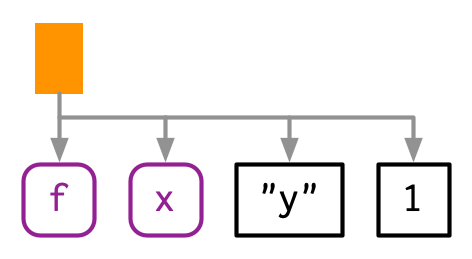
\includegraphics[width=1.97in]{diagrams/expressions/simple} \end{center}
\item
  With \texttt{lobstr::ast()}:

\begin{Shaded}
\begin{Highlighting}[]
\NormalTok{lobstr}\OperatorTok{::}\KeywordTok{ast}\NormalTok{(}\KeywordTok{f}\NormalTok{(x, }\StringTok{"y"}\NormalTok{, }\DecValTok{1}\NormalTok{))}
\CommentTok{#> █─f }
\CommentTok{#> ├─x }
\CommentTok{#> ├─"y" }
\CommentTok{#> └─1}
\end{Highlighting}
\end{Shaded}
\end{itemize}

Both approaches share conventions as much as possible:

\begin{itemize}
\item
  The leaves of the tree are either symbols, like \texttt{f} and \texttt{x}, or constants,
  like \texttt{1} or \texttt{"y"}. Symbols are drawn in purple and have rounded corners.
  Constants have black borders and square corners. Strings and symbols are
  easily confused, so strings are always surrounded in quotes.
\item
  The branches of the tree are call objects, which represent function calls,
  and are drawn as orange rectangles. The first child (\texttt{f}) is the function
  that gets called; the second and subsequent children (\texttt{x}, \texttt{"y"}, and \texttt{1})
  are the arguments to that function.
\end{itemize}

Colours will be shown when \emph{you} call \texttt{ast()}, but do not appear in the book for complicated technical reasons.

The above example only contained one function call, making for a very shallow tree. Most expressions will contain considerably more calls, creating trees with multiple levels. For example, consider the AST for \texttt{f(g(1,\ 2),\ h(3,\ 4,\ i()))}:

\begin{center}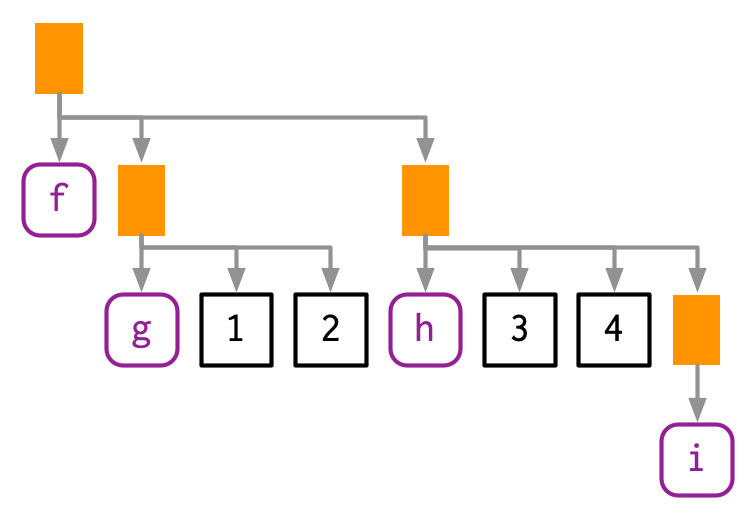
\includegraphics[width=3.15in]{diagrams/expressions/complicated} \end{center}

\begin{Shaded}
\begin{Highlighting}[]
\NormalTok{lobstr}\OperatorTok{::}\KeywordTok{ast}\NormalTok{(}\KeywordTok{f}\NormalTok{(}\KeywordTok{g}\NormalTok{(}\DecValTok{1}\NormalTok{, }\DecValTok{2}\NormalTok{), }\KeywordTok{h}\NormalTok{(}\DecValTok{3}\NormalTok{, }\DecValTok{4}\NormalTok{, }\KeywordTok{i}\NormalTok{())))}
\CommentTok{#> █─f }
\CommentTok{#> ├─█─g }
\CommentTok{#> │ ├─1 }
\CommentTok{#> │ └─2 }
\CommentTok{#> └─█─h }
\CommentTok{#>   ├─3 }
\CommentTok{#>   ├─4 }
\CommentTok{#>   └─█─i}
\end{Highlighting}
\end{Shaded}

You can read the hand-drawn diagrams from left-to-right (ignoring vertical position), and the lobstr-drawn diagrams from top-to-bottom (ignoring horizontal position). The depth within the tree is determined by the nesting of function calls. This also determines evaluation order, as evaluation generally proceeds from deepest-to-shallowest, but this is not guaranteed because of lazy evaluation (Section \ref{lazy-evaluation}). Also note the appearance of \texttt{i()}, a function call with no arguments; it's a branch with a single (symbol) leaf.

\hypertarget{non-code-components}{%
\subsection{Non-code components}\label{non-code-components}}

\index{ASTs!non-code}

You might have wondered what makes these \emph{abstract} syntax trees. They are abstract because they only capture important structural details of the code, not whitespace or comments:

\begin{Shaded}
\begin{Highlighting}[]
\KeywordTok{ast}\NormalTok{(}
  \KeywordTok{f}\NormalTok{(x,  y)  }\CommentTok{# important!}
\NormalTok{)}
\CommentTok{#> █─f }
\CommentTok{#> ├─x }
\CommentTok{#> └─y}
\end{Highlighting}
\end{Shaded}

There's only one place where whitespace affects the AST:

\begin{Shaded}
\begin{Highlighting}[]
\NormalTok{lobstr}\OperatorTok{::}\KeywordTok{ast}\NormalTok{(y <-}\StringTok{ }\NormalTok{x)}
\CommentTok{#> █─`<-` }
\CommentTok{#> ├─y }
\CommentTok{#> └─x}
\NormalTok{lobstr}\OperatorTok{::}\KeywordTok{ast}\NormalTok{(y }\OperatorTok{<}\StringTok{ }\OperatorTok{-}\NormalTok{x)}
\CommentTok{#> █─`<` }
\CommentTok{#> ├─y }
\CommentTok{#> └─█─`-` }
\CommentTok{#>   └─x}
\end{Highlighting}
\end{Shaded}

\hypertarget{infix-calls}{%
\subsection{Infix calls}\label{infix-calls}}

\index{ASTs!infix calls}

Every call in R can be written in tree form because any call can be written in prefix form (Section \ref{prefix-transform}). Take \texttt{y\ \textless{}-\ x\ *\ 10} again: what are the functions that are being called? It is not as easy to spot as \texttt{f(x,\ 1)} because this expression contains two infix calls: \texttt{\textless{}-} and \texttt{*}. That means that these two lines of code are equivalent:

\begin{Shaded}
\begin{Highlighting}[]
\NormalTok{y <-}\StringTok{ }\NormalTok{x }\OperatorTok{*}\StringTok{ }\DecValTok{10}
\StringTok{`}\DataTypeTok{<-}\StringTok{`}\NormalTok{(y, }\StringTok{`}\DataTypeTok{*}\StringTok{`}\NormalTok{(x, }\DecValTok{10}\NormalTok{))}
\end{Highlighting}
\end{Shaded}

And they both have this AST\footnote{The names of non-prefix functions are non-syntactic so I surround them with \texttt{\textasciigrave{}\textasciigrave{}}, as in Section \ref{non-syntactic}.}:

\begin{center}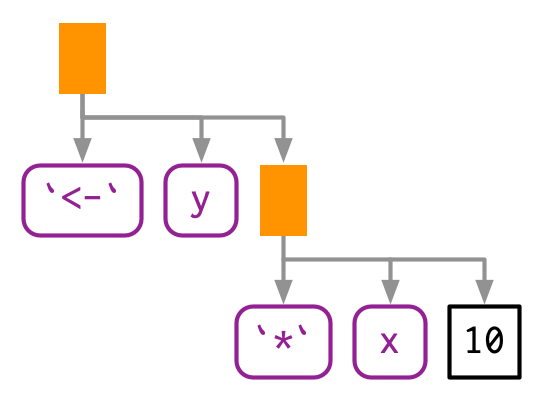
\includegraphics[width=2.26in]{diagrams/expressions/prefix} \end{center}

\begin{Shaded}
\begin{Highlighting}[]
\NormalTok{lobstr}\OperatorTok{::}\KeywordTok{ast}\NormalTok{(y <-}\StringTok{ }\NormalTok{x }\OperatorTok{*}\StringTok{ }\DecValTok{10}\NormalTok{)}
\CommentTok{#> █─`<-` }
\CommentTok{#> ├─y }
\CommentTok{#> └─█─`*` }
\CommentTok{#>   ├─x }
\CommentTok{#>   └─10}
\end{Highlighting}
\end{Shaded}

There really is no difference between the ASTs, and if you generate an expression with prefix calls, R will still print it in infix form:

\begin{Shaded}
\begin{Highlighting}[]
\KeywordTok{expr}\NormalTok{(}\StringTok{`}\DataTypeTok{<-}\StringTok{`}\NormalTok{(y, }\StringTok{`}\DataTypeTok{*}\StringTok{`}\NormalTok{(x, }\DecValTok{10}\NormalTok{)))}
\CommentTok{#> y <- x * 10}
\end{Highlighting}
\end{Shaded}

The order in which infix operators are applied is governed by a set of rules called operator precedence, and we'll \texttt{lobstr::ast()} to explore them in Section \ref{operator-precedence}.

\hypertarget{exercises}{%
\subsection{Exercises}\label{exercises}}

\begin{enumerate}
\def\labelenumi{\arabic{enumi}.}
\item
  Reconstruct the code represented by the trees below:

\begin{verbatim}
#> █─f 
#> └─█─g 
#>   └─█─h
#> █─`+` 
#> ├─█─`+` 
#> │ ├─1 
#> │ └─2 
#> └─3
#> █─`*` 
#> ├─█─`(` 
#> │ └─█─`+` 
#> │   ├─x 
#> │   └─y 
#> └─z
\end{verbatim}
\item
  Draw the following trees by hand then check your answers with
  \texttt{lobstr::ast()}.

\begin{Shaded}
\begin{Highlighting}[]
\KeywordTok{f}\NormalTok{(}\KeywordTok{g}\NormalTok{(}\KeywordTok{h}\NormalTok{(}\KeywordTok{i}\NormalTok{(}\DecValTok{1}\NormalTok{, }\DecValTok{2}\NormalTok{, }\DecValTok{3}\NormalTok{))))}
\KeywordTok{f}\NormalTok{(}\DecValTok{1}\NormalTok{, }\KeywordTok{g}\NormalTok{(}\DecValTok{2}\NormalTok{, }\KeywordTok{h}\NormalTok{(}\DecValTok{3}\NormalTok{, }\KeywordTok{i}\NormalTok{())))}
\KeywordTok{f}\NormalTok{(}\KeywordTok{g}\NormalTok{(}\DecValTok{1}\NormalTok{, }\DecValTok{2}\NormalTok{), }\KeywordTok{h}\NormalTok{(}\DecValTok{3}\NormalTok{, }\KeywordTok{i}\NormalTok{(}\DecValTok{4}\NormalTok{, }\DecValTok{5}\NormalTok{)))}
\end{Highlighting}
\end{Shaded}
\item
  What's happening with the ASTs below? (Hint: carefully read \texttt{?"\^{}"})

\begin{Shaded}
\begin{Highlighting}[]
\NormalTok{lobstr}\OperatorTok{::}\KeywordTok{ast}\NormalTok{(}\StringTok{`}\DataTypeTok{x}\StringTok{`} \OperatorTok{+}\StringTok{ `}\DataTypeTok{y}\StringTok{`}\NormalTok{)}
\CommentTok{#> █─`+` }
\CommentTok{#> ├─x }
\CommentTok{#> └─y}
\NormalTok{lobstr}\OperatorTok{::}\KeywordTok{ast}\NormalTok{(x }\OperatorTok{**}\StringTok{ }\NormalTok{y)}
\CommentTok{#> █─`^` }
\CommentTok{#> ├─x }
\CommentTok{#> └─y}
\NormalTok{lobstr}\OperatorTok{::}\KeywordTok{ast}\NormalTok{(}\DecValTok{1}\NormalTok{ ->}\StringTok{ }\NormalTok{x)}
\CommentTok{#> █─`<-` }
\CommentTok{#> ├─x }
\CommentTok{#> └─1}
\end{Highlighting}
\end{Shaded}
\item
  What is special about the AST below? (Hint: re-read Section
  \ref{fun-components})

\begin{Shaded}
\begin{Highlighting}[]
\NormalTok{lobstr}\OperatorTok{::}\KeywordTok{ast}\NormalTok{(}\ControlFlowTok{function}\NormalTok{(}\DataTypeTok{x =} \DecValTok{1}\NormalTok{, }\DataTypeTok{y =} \DecValTok{2}\NormalTok{) \{\})}
\CommentTok{#> █─`function` }
\CommentTok{#> ├─█─x = 1 }
\CommentTok{#> │ └─y = 2 }
\CommentTok{#> ├─█─`\{` }
\CommentTok{#> └─<inline srcref>}
\end{Highlighting}
\end{Shaded}
\item
  What does the call tree of an \texttt{if} statement with multiple \texttt{else\ if}
  conditions look like? Why?
\end{enumerate}

\hypertarget{expression-details}{%
\section{Expressions}\label{expression-details}}

\index{expressions}
\indexc{expr()}

Collectively, the data structures present in the AST are called expressions. An \textbf{expression} is any member of the set of base types created by parsing code: constant scalars, symbols, call objects, and pairlists. These are the data structures used to represent captured code from \texttt{expr()}, and \texttt{is\_expression(expr(...))} is always true\footnote{It is \emph{possible} to insert any other base object into an expression, but this is unusual and only needed in rare circumstances. We'll come back to that idea in Section \ref{non-standard-ast}.}. Constants, symbols and call objects are the most important, and are discussed below. Pairlists and empty symbols are more specialised and we'll come back to them in Sections \ref{pairlists} and Section \ref{empty-symbol}.

NB: In base R documentation ``expression'' is used to mean two things. As well as the definition above, expression is also used to refer to the type of object returned by \texttt{expression()} and \texttt{parse()}, which are basically lists of expressions as defined above. In this book I'll call these \textbf{expression vectors}, and I'll come back to them in Section \ref{expression-vectors}.

\hypertarget{constants}{%
\subsection{Constants}\label{constants}}

\index{constants}
\index{scalars}

Scalar constants are the simplest component of the AST. More precisely, a \textbf{constant} is either \texttt{NULL} or a length-1 atomic vector (or scalar, Section \ref{scalars}) like \texttt{TRUE}, \texttt{1L}, \texttt{2.5} or \texttt{"x"}. You can test for a constant with \texttt{rlang::is\_syntactic\_literal()}.

Constants are ``self-quoting'' in the sense that the expression used to represent a constant is the constant itself:

\begin{Shaded}
\begin{Highlighting}[]
\KeywordTok{identical}\NormalTok{(}\KeywordTok{expr}\NormalTok{(}\OtherTok{TRUE}\NormalTok{), }\OtherTok{TRUE}\NormalTok{)}
\CommentTok{#> [1] TRUE}
\KeywordTok{identical}\NormalTok{(}\KeywordTok{expr}\NormalTok{(}\DecValTok{1}\NormalTok{), }\DecValTok{1}\NormalTok{)}
\CommentTok{#> [1] TRUE}
\KeywordTok{identical}\NormalTok{(}\KeywordTok{expr}\NormalTok{(2L), 2L)}
\CommentTok{#> [1] TRUE}
\KeywordTok{identical}\NormalTok{(}\KeywordTok{expr}\NormalTok{(}\StringTok{"x"}\NormalTok{), }\StringTok{"x"}\NormalTok{)}
\CommentTok{#> [1] TRUE}
\end{Highlighting}
\end{Shaded}

\hypertarget{symbols}{%
\subsection{Symbols}\label{symbols}}

\index{symbols}
\index{names|see {symbols}}
\indexc{sym()}

A \textbf{symbol} represents the name of an object like \texttt{x}, \texttt{mtcars}, or \texttt{mean}. In base R, the terms symbol and name are used interchangeably (i.e. \texttt{is.name()} is identical to \texttt{is.symbol()}), but in this book I used symbol consistently because ``name'' has many other meanings.

You can create a symbol in two ways: by capturing code that references an object with \texttt{expr()}, or turning a string into a symbol with \texttt{rlang::sym()}:

\begin{Shaded}
\begin{Highlighting}[]
\KeywordTok{expr}\NormalTok{(x)}
\CommentTok{#> x}
\KeywordTok{sym}\NormalTok{(}\StringTok{"x"}\NormalTok{)}
\CommentTok{#> x}
\end{Highlighting}
\end{Shaded}

\indexc{as\_string()}

You can turn a symbol back into a string with \texttt{as.character()} or \texttt{rlang::as\_string()}. \texttt{as\_string()} has the advantage of clearly signalling that you'll get a character vector of length 1.

\begin{Shaded}
\begin{Highlighting}[]
\KeywordTok{as_string}\NormalTok{(}\KeywordTok{expr}\NormalTok{(x))}
\CommentTok{#> [1] "x"}
\end{Highlighting}
\end{Shaded}

You can recognise a symbol because it's printed without quotes, \texttt{str()} tells you that it's a symbol, and \texttt{is.symbol()} is \texttt{TRUE}:

\begin{Shaded}
\begin{Highlighting}[]
\KeywordTok{str}\NormalTok{(}\KeywordTok{expr}\NormalTok{(x))}
\CommentTok{#>  symbol x}
\KeywordTok{is.symbol}\NormalTok{(}\KeywordTok{expr}\NormalTok{(x))}
\CommentTok{#> [1] TRUE}
\end{Highlighting}
\end{Shaded}

The symbol type is not vectorised, i.e.~a symbol is always length 1. If you want multiple symbols, you'll need to put them in a list, using (e.g.) \texttt{rlang::syms()}.

\hypertarget{calls}{%
\subsection{Calls}\label{calls}}

\index{call objects}
\index{language objects!see {call objects}}

A \textbf{call object} represents a captured function call. Call objects are a special type of list\footnote{More precisely, they're pairlists, Section \ref{pairlists}, but this distinction rarely matters.} where the first component specifies the function to call (usually a symbol), and the remaining elements are the arguments for that call. Call objects create branches in the AST, because calls can be nested inside other calls.

You can identify a call object when printed because it looks just like a function call. Confusingly \texttt{typeof()} and \texttt{str()} print ``language''\footnote{Avoid \texttt{is.language()} which returns \texttt{TRUE} for symbols, calls, and expression vectors.} for call objects, but \texttt{is.call()} returns \texttt{TRUE}:

\begin{Shaded}
\begin{Highlighting}[]
\NormalTok{lobstr}\OperatorTok{::}\KeywordTok{ast}\NormalTok{(}\KeywordTok{read.table}\NormalTok{(}\StringTok{"important.csv"}\NormalTok{, }\DataTypeTok{row.names =} \OtherTok{FALSE}\NormalTok{))}
\CommentTok{#> █─read.table }
\CommentTok{#> ├─"important.csv" }
\CommentTok{#> └─row.names = FALSE}
\NormalTok{x <-}\StringTok{ }\KeywordTok{expr}\NormalTok{(}\KeywordTok{read.table}\NormalTok{(}\StringTok{"important.csv"}\NormalTok{, }\DataTypeTok{row.names =} \OtherTok{FALSE}\NormalTok{))}

\KeywordTok{typeof}\NormalTok{(x)}
\CommentTok{#> [1] "language"}
\KeywordTok{is.call}\NormalTok{(x)}
\CommentTok{#> [1] TRUE}
\end{Highlighting}
\end{Shaded}

\hypertarget{subsetting}{%
\subsubsection{Subsetting}\label{subsetting}}

\index{call objects!subsetting}

Calls generally behave like lists, i.e.~you can use standard subsetting tools. The first element of the call object is the function to call, which is a usually a symbol:

\begin{Shaded}
\begin{Highlighting}[]
\NormalTok{x[[}\DecValTok{1}\NormalTok{]]}
\CommentTok{#> read.table}
\KeywordTok{is.symbol}\NormalTok{(x[[}\DecValTok{1}\NormalTok{]])}
\CommentTok{#> [1] TRUE}
\end{Highlighting}
\end{Shaded}

The remainder of the elements are the arguments:

\begin{Shaded}
\begin{Highlighting}[]
\KeywordTok{as.list}\NormalTok{(x[}\OperatorTok{-}\DecValTok{1}\NormalTok{])}
\CommentTok{#> [[1]]}
\CommentTok{#> [1] "important.csv"}
\CommentTok{#> }
\CommentTok{#> $row.names}
\CommentTok{#> [1] FALSE}
\end{Highlighting}
\end{Shaded}

You can extract individual arguments with \texttt{{[}{[}} or, if named, \texttt{\$}:

\begin{Shaded}
\begin{Highlighting}[]
\NormalTok{x[[}\DecValTok{2}\NormalTok{]]}
\CommentTok{#> [1] "important.csv"}
\NormalTok{x}\OperatorTok{$}\NormalTok{row.names}
\CommentTok{#> [1] FALSE}
\end{Highlighting}
\end{Shaded}

You can determine the number of arguments in a call object by subtracting 1 from its length:

\begin{Shaded}
\begin{Highlighting}[]
\KeywordTok{length}\NormalTok{(x) }\OperatorTok{-}\StringTok{ }\DecValTok{1}
\CommentTok{#> [1] 2}
\end{Highlighting}
\end{Shaded}

Extracting specific arguments from calls is challenging because of R's flexible rules for argument matching: it could potentially be in any location, with the full name, with an abbreviated name, or with no name. To work around this problem, you can use \texttt{rlang::call\_standardise()} which standardises all arguments to use the full name:
\indexc{standardise\_call()}

\begin{Shaded}
\begin{Highlighting}[]
\NormalTok{rlang}\OperatorTok{::}\KeywordTok{call_standardise}\NormalTok{(x)}
\CommentTok{#> read.table(file = "important.csv", row.names = FALSE)}
\end{Highlighting}
\end{Shaded}

(NB: If the function uses \texttt{...} it's not possible to standardise all arguments.)

Calls can be modified in the same way as lists:

\begin{Shaded}
\begin{Highlighting}[]
\NormalTok{x}\OperatorTok{$}\NormalTok{header <-}\StringTok{ }\OtherTok{TRUE}
\NormalTok{x}
\CommentTok{#> read.table("important.csv", row.names = FALSE, header = TRUE)}
\end{Highlighting}
\end{Shaded}

\hypertarget{function-position}{%
\subsubsection{Function position}\label{function-position}}

\index{call objects!function component}

The first element of the call object is the \textbf{function position}. This contains the function that will be called when the object is evaluated, and is usually a symbol\footnote{Peculiarly, it can also be a number, as in the expression \texttt{3()}. But this call will always fail to evaluate because a number is not a function.}:

\begin{Shaded}
\begin{Highlighting}[]
\NormalTok{lobstr}\OperatorTok{::}\KeywordTok{ast}\NormalTok{(}\KeywordTok{foo}\NormalTok{())}
\CommentTok{#> █─foo}
\end{Highlighting}
\end{Shaded}

While R allows you to surround the name of the function with quotes, the parser converts it to a symbol:

\begin{Shaded}
\begin{Highlighting}[]
\NormalTok{lobstr}\OperatorTok{::}\KeywordTok{ast}\NormalTok{(}\StringTok{"foo"}\NormalTok{())}
\CommentTok{#> █─foo}
\end{Highlighting}
\end{Shaded}

However, sometimes the function doesn't exist in the current environment and you need to do some computation to retrieve it: for example, if the function is in another package, is a method of an R6 object, or is created by a function factory. In this case, the function position will be occupied by another call:

\begin{Shaded}
\begin{Highlighting}[]
\NormalTok{lobstr}\OperatorTok{::}\KeywordTok{ast}\NormalTok{(pkg}\OperatorTok{::}\KeywordTok{foo}\NormalTok{(}\DecValTok{1}\NormalTok{))}
\CommentTok{#> █─█─`::` }
\CommentTok{#> │ ├─pkg }
\CommentTok{#> │ └─foo }
\CommentTok{#> └─1}
\NormalTok{lobstr}\OperatorTok{::}\KeywordTok{ast}\NormalTok{(obj}\OperatorTok{$}\KeywordTok{foo}\NormalTok{(}\DecValTok{1}\NormalTok{))}
\CommentTok{#> █─█─`$` }
\CommentTok{#> │ ├─obj }
\CommentTok{#> │ └─foo }
\CommentTok{#> └─1}
\NormalTok{lobstr}\OperatorTok{::}\KeywordTok{ast}\NormalTok{(}\KeywordTok{foo}\NormalTok{(}\DecValTok{1}\NormalTok{)(}\DecValTok{2}\NormalTok{))}
\CommentTok{#> █─█─foo }
\CommentTok{#> │ └─1 }
\CommentTok{#> └─2}
\end{Highlighting}
\end{Shaded}

\begin{center}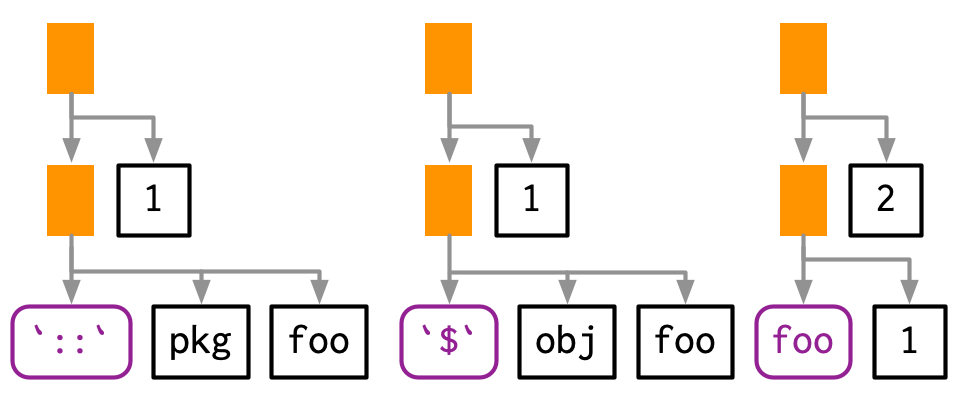
\includegraphics[width=4.03in]{diagrams/expressions/call-call} \end{center}

\hypertarget{call2}{%
\subsubsection{Constructing}\label{call2}}

\index{call objects!constructing}
\indexc{call2()}

You can construct a call object from its components using \texttt{rlang::call2()}. The first argument is the name of the function to call (either as a string, a symbol, or another call). The remaining arguments will be passed along to the call:

\begin{Shaded}
\begin{Highlighting}[]
\KeywordTok{call2}\NormalTok{(}\StringTok{"mean"}\NormalTok{, }\DataTypeTok{x =} \KeywordTok{expr}\NormalTok{(x), }\DataTypeTok{na.rm =} \OtherTok{TRUE}\NormalTok{)}
\CommentTok{#> mean(x = x, na.rm = TRUE)}
\KeywordTok{call2}\NormalTok{(}\KeywordTok{expr}\NormalTok{(base}\OperatorTok{::}\NormalTok{mean), }\DataTypeTok{x =} \KeywordTok{expr}\NormalTok{(x), }\DataTypeTok{na.rm =} \OtherTok{TRUE}\NormalTok{)}
\CommentTok{#> base::mean(x = x, na.rm = TRUE)}
\end{Highlighting}
\end{Shaded}

Infix calls created in this way still print as usual.

\begin{Shaded}
\begin{Highlighting}[]
\KeywordTok{call2}\NormalTok{(}\StringTok{"<-"}\NormalTok{, }\KeywordTok{expr}\NormalTok{(x), }\DecValTok{10}\NormalTok{)}
\CommentTok{#> x <- 10}
\end{Highlighting}
\end{Shaded}

Using \texttt{call2()} to create complex expressions is a bit clunky. You'll learn another technique in Chapter \ref{quasiquotation}.

\hypertarget{summary}{%
\subsection{Summary}\label{summary}}

The following table summarises the appearance of the different expression subtypes in \texttt{str()} and \texttt{typeof()}:

\begin{longtable}[]{@{}lll@{}}
\toprule
& \texttt{str()} & \texttt{typeof()}\tabularnewline
\midrule
\endhead
Scalar constant & \texttt{logi}/\texttt{int}/\texttt{num}/\texttt{chr} & \texttt{logical}/\texttt{integer}/\texttt{double}/\texttt{character}\tabularnewline
Symbol & \texttt{symbol} & \texttt{symbol}\tabularnewline
Call object & \texttt{language} & \texttt{language}\tabularnewline
Pairlist & Dotted pair list & \texttt{pairlist}\tabularnewline
Expression vector & \texttt{expression()} & \texttt{expression}\tabularnewline
\bottomrule
\end{longtable}

Both base R and rlang provide functions for testing for each type of input, although the types covered are slightly different. You can easily tell them apart because all the base functions start with \texttt{is.} and the rlang functions start with \texttt{is\_}.

\begin{longtable}[]{@{}lll@{}}
\toprule
& base & rlang\tabularnewline
\midrule
\endhead
Scalar constant & --- & \texttt{is\_syntactic\_literal()}\tabularnewline
Symbol & \texttt{is.symbol()} & \texttt{is\_symbol()}\tabularnewline
Call object & \texttt{is.call()} & \texttt{is\_call()}\tabularnewline
Pairlist & \texttt{is.pairlist()} & \texttt{is\_pairlist()}\tabularnewline
Expression vector & \texttt{is.expression()} & ---\tabularnewline
\bottomrule
\end{longtable}

\hypertarget{exercises-1}{%
\subsection{Exercises}\label{exercises-1}}

\begin{enumerate}
\def\labelenumi{\arabic{enumi}.}
\item
  Which two of the six types of atomic vector can't appear in an expression?
  Why? Similarly, why can't you create an expression that contains an atomic
  vector of length greater than one?
\item
  What happens when you subset a call object to remove the first element?
  e.g. \texttt{expr(read.csv("foo.csv",\ header\ =\ TRUE)){[}-1{]}}. Why?
\item
  Describe the differences between the following call objects.

\begin{Shaded}
\begin{Highlighting}[]
\NormalTok{x <-}\StringTok{ }\DecValTok{1}\OperatorTok{:}\DecValTok{10}

\KeywordTok{call2}\NormalTok{(median, x, }\DataTypeTok{na.rm =} \OtherTok{TRUE}\NormalTok{)}
\KeywordTok{call2}\NormalTok{(}\KeywordTok{expr}\NormalTok{(median), x, }\DataTypeTok{na.rm =} \OtherTok{TRUE}\NormalTok{)}
\KeywordTok{call2}\NormalTok{(median, }\KeywordTok{expr}\NormalTok{(x), }\DataTypeTok{na.rm =} \OtherTok{TRUE}\NormalTok{)}
\KeywordTok{call2}\NormalTok{(}\KeywordTok{expr}\NormalTok{(median), }\KeywordTok{expr}\NormalTok{(x), }\DataTypeTok{na.rm =} \OtherTok{TRUE}\NormalTok{)}
\end{Highlighting}
\end{Shaded}
\item
  \texttt{rlang::call\_standardise()} doesn't work so well for the following calls.
  Why? What makes \texttt{mean()} special?

\begin{Shaded}
\begin{Highlighting}[]
\KeywordTok{call_standardise}\NormalTok{(}\KeywordTok{quote}\NormalTok{(}\KeywordTok{mean}\NormalTok{(}\DecValTok{1}\OperatorTok{:}\DecValTok{10}\NormalTok{, }\DataTypeTok{na.rm =} \OtherTok{TRUE}\NormalTok{)))}
\CommentTok{#> mean(x = 1:10, na.rm = TRUE)}
\KeywordTok{call_standardise}\NormalTok{(}\KeywordTok{quote}\NormalTok{(}\KeywordTok{mean}\NormalTok{(}\DataTypeTok{n =}\NormalTok{ T, }\DecValTok{1}\OperatorTok{:}\DecValTok{10}\NormalTok{)))}
\CommentTok{#> mean(x = 1:10, n = T)}
\KeywordTok{call_standardise}\NormalTok{(}\KeywordTok{quote}\NormalTok{(}\KeywordTok{mean}\NormalTok{(}\DataTypeTok{x =} \DecValTok{1}\OperatorTok{:}\DecValTok{10}\NormalTok{, , }\OtherTok{TRUE}\NormalTok{)))}
\CommentTok{#> mean(x = 1:10, , TRUE)}
\end{Highlighting}
\end{Shaded}
\item
  Why does this code not make sense?

\begin{Shaded}
\begin{Highlighting}[]
\NormalTok{x <-}\StringTok{ }\KeywordTok{expr}\NormalTok{(}\KeywordTok{foo}\NormalTok{(}\DataTypeTok{x =} \DecValTok{1}\NormalTok{))}
\KeywordTok{names}\NormalTok{(x) <-}\StringTok{ }\KeywordTok{c}\NormalTok{(}\StringTok{"x"}\NormalTok{, }\StringTok{"y"}\NormalTok{)}
\end{Highlighting}
\end{Shaded}
\item
  Construct the expression \texttt{if(x\ \textgreater{}\ 1)\ "a"\ else\ "b"} using multiple calls to
  \texttt{call2()}. How does the code structure reflect the structure of the AST?
\end{enumerate}

\hypertarget{grammar}{%
\section{Parsing and grammar}\label{grammar}}

\index{grammar}

We've talked a lot about expressions and the AST, but not about how expressions are created from code that you type (like \texttt{"x\ +\ y"}). The process by which a computer language takes a string and constructs an expression is called \textbf{parsing}, and is governed by a set of rules known as a \textbf{grammar}. In this section, we'll use \texttt{lobstr::ast()} to explore some of the details of R's grammar, and then show how you can transform back and forth between expressions and strings.

\hypertarget{operator-precedence}{%
\subsection{Operator precedence}\label{operator-precedence}}

\index{operator precedence}

Infix functions introduce two sources of ambiguity\footnote{This ambiguity does not exist in languages with only prefix or postfix calls. It's interesting to compare a simple arithmetic operation in Lisp (prefix) and Forth (postfix). In Lisp you'd write \texttt{(*\ (+\ 1\ 2)\ 3))}; this avoids ambiguity by requiring parentheses everywhere. In Forth, you'd write \texttt{1\ 2\ +\ 3\ *}; this doesn't require any parentheses, but does require more thought when reading.}. The first source of ambiguity arises from infix functions: what does \texttt{1\ +\ 2\ *\ 3} yield? Do you get 9 (i.e. \texttt{(1\ +\ 2)\ *\ 3}), or 7 (i.e. \texttt{1\ +\ (2\ *\ 3)})? In other words, which of the two possible parse trees below does R use?

\begin{center}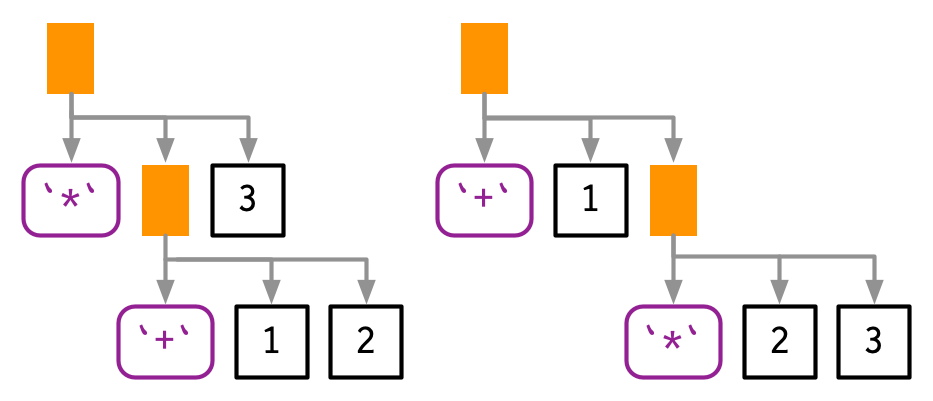
\includegraphics[width=3.89in]{diagrams/expressions/ambig-order} \end{center}

Programming languages use conventions called \textbf{operator precedence} to resolve this ambiguity. We can use \texttt{ast()} to see what R does:

\begin{Shaded}
\begin{Highlighting}[]
\NormalTok{lobstr}\OperatorTok{::}\KeywordTok{ast}\NormalTok{(}\DecValTok{1} \OperatorTok{+}\StringTok{ }\DecValTok{2} \OperatorTok{*}\StringTok{ }\DecValTok{3}\NormalTok{)}
\CommentTok{#> █─`+` }
\CommentTok{#> ├─1 }
\CommentTok{#> └─█─`*` }
\CommentTok{#>   ├─2 }
\CommentTok{#>   └─3}
\end{Highlighting}
\end{Shaded}

Predicting the precedence of arithmetic operations is usually easy because it's drilled into you in school and is consistent across the vast majority of programming languages.

Predicting the precedence of other operators is harder. There's one particularly surprising case in R: \texttt{!} has a much lower precedence (i.e.~it binds less tightly) than you might expect. This allows you to write useful operations like:

\begin{Shaded}
\begin{Highlighting}[]
\NormalTok{lobstr}\OperatorTok{::}\KeywordTok{ast}\NormalTok{(}\OperatorTok{!}\NormalTok{x }\OperatorTok\StringTok{ }\NormalTok{y)}
\CommentTok{#> █─`!` }
\CommentTok{#> └─█─`%in%` }
\CommentTok{#>   ├─x }
\CommentTok{#>   └─y}
\end{Highlighting}
\end{Shaded}

R has over 30 infix operators divided into 18 precedence groups. While the details are described in \texttt{?Syntax}, very few people have memorised the complete ordering. If there's any confusion, use parentheses!

\begin{Shaded}
\begin{Highlighting}[]
\NormalTok{lobstr}\OperatorTok{::}\KeywordTok{ast}\NormalTok{((}\DecValTok{1} \OperatorTok{+}\StringTok{ }\DecValTok{2}\NormalTok{) }\OperatorTok{*}\StringTok{ }\DecValTok{3}\NormalTok{)}
\CommentTok{#> █─`*` }
\CommentTok{#> ├─█─`(` }
\CommentTok{#> │ └─█─`+` }
\CommentTok{#> │   ├─1 }
\CommentTok{#> │   └─2 }
\CommentTok{#> └─3}
\end{Highlighting}
\end{Shaded}

Note the appearance of the parentheses in the AST as a call to the \texttt{(} function.

\hypertarget{associativity}{%
\subsection{Associativity}\label{associativity}}

The second source of ambiguity is introduced by repeated usage of the same infix function. For example, is \texttt{1\ +\ 2\ +\ 3} equivalent to \texttt{(1\ +\ 2)\ +\ 3} or to \texttt{1\ +\ (2\ +\ 3)}? This normally doesn't matter because \texttt{x\ +\ (y\ +\ z)\ ==\ (x\ +\ y)\ +\ z}, i.e.~addition is associative, but is needed because some S3 classes define \texttt{+} in a non-associative way. For example, ggplot2 overloads \texttt{+} to build up a complex plot from simple pieces; this is non-associative because earlier layers are drawn underneath later layers (i.e. \texttt{geom\_point()} + \texttt{geom\_smooth()} does not yield the same plot as \texttt{geom\_smooth()} + \texttt{geom\_point()}).

In R, most operators are \textbf{left-associative}, i.e.~the operations on the left are evaluated first:

\begin{Shaded}
\begin{Highlighting}[]
\NormalTok{lobstr}\OperatorTok{::}\KeywordTok{ast}\NormalTok{(}\DecValTok{1} \OperatorTok{+}\StringTok{ }\DecValTok{2} \OperatorTok{+}\StringTok{ }\DecValTok{3}\NormalTok{)}
\CommentTok{#> █─`+` }
\CommentTok{#> ├─█─`+` }
\CommentTok{#> │ ├─1 }
\CommentTok{#> │ └─2 }
\CommentTok{#> └─3}
\end{Highlighting}
\end{Shaded}

There are two exceptions: exponentiation and assignment.

\begin{Shaded}
\begin{Highlighting}[]
\NormalTok{lobstr}\OperatorTok{::}\KeywordTok{ast}\NormalTok{(}\DecValTok{2}\OperatorTok{^}\DecValTok{2}\OperatorTok{^}\DecValTok{3}\NormalTok{)}
\CommentTok{#> █─`^` }
\CommentTok{#> ├─2 }
\CommentTok{#> └─█─`^` }
\CommentTok{#>   ├─2 }
\CommentTok{#>   └─3}
\NormalTok{lobstr}\OperatorTok{::}\KeywordTok{ast}\NormalTok{(x <-}\StringTok{ }\NormalTok{y <-}\StringTok{ }\NormalTok{z)}
\CommentTok{#> █─`<-` }
\CommentTok{#> ├─x }
\CommentTok{#> └─█─`<-` }
\CommentTok{#>   ├─y }
\CommentTok{#>   └─z}
\end{Highlighting}
\end{Shaded}

\hypertarget{parsing}{%
\subsection{Parsing and deparsing}\label{parsing}}

\index{parsing}
\indexc{parsing!parse\_expr@\texttt{parse\_expr()}}

Most of the time you type code into the console, and R takes care of turning the characters you've typed into an AST. But occasionally you have code stored in a string, and you want to parse it yourself. You can do so using \texttt{rlang::parse\_expr()}:

\begin{Shaded}
\begin{Highlighting}[]
\NormalTok{x1 <-}\StringTok{ "y <- x + 10"}
\NormalTok{x1}
\CommentTok{#> [1] "y <- x + 10"}
\KeywordTok{is.call}\NormalTok{(x1)}
\CommentTok{#> [1] FALSE}

\NormalTok{x2 <-}\StringTok{ }\NormalTok{rlang}\OperatorTok{::}\KeywordTok{parse_expr}\NormalTok{(x1)}
\NormalTok{x2}
\CommentTok{#> y <- x + 10}
\KeywordTok{is.call}\NormalTok{(x2)}
\CommentTok{#> [1] TRUE}
\end{Highlighting}
\end{Shaded}

\texttt{parse\_expr()} always returns a single expression. If you have multiple expression separated by \texttt{;} or \texttt{\textbackslash{}n}, you'll need to use \texttt{rlang::parse\_exprs()}. It returns a list of expressions:

\begin{Shaded}
\begin{Highlighting}[]
\NormalTok{x3 <-}\StringTok{ "a <- 1; a + 1"}
\NormalTok{rlang}\OperatorTok{::}\KeywordTok{parse_exprs}\NormalTok{(x3)}
\CommentTok{#> [[1]]}
\CommentTok{#> a <- 1}
\CommentTok{#> }
\CommentTok{#> [[2]]}
\CommentTok{#> a + 1}
\end{Highlighting}
\end{Shaded}

If you find yourself working with strings containing code very frequently, you should reconsider your process. Read Chapter \ref{quasiquotation} and consider if you can instead more safely generate expressions using quasiquotation.

\indexc{parsing!parse@\texttt{parse()}}

The base equivalent to \texttt{parse\_exprs()} is \texttt{parse()}. It is a little harder to use because it's specialised for parsing R code stored in files. You need supply your string to the \texttt{text} argument and it returns an expression vector (Section \ref{expression-vectors}). I recommend turning the output into a list:

\begin{Shaded}
\begin{Highlighting}[]
\KeywordTok{as.list}\NormalTok{(}\KeywordTok{parse}\NormalTok{(}\DataTypeTok{text =}\NormalTok{ x1))}
\CommentTok{#> [[1]]}
\CommentTok{#> y <- x + 10}
\end{Highlighting}
\end{Shaded}

\index{deparsing}
\indexc{expr\_text()}

The inverse of parsing is \textbf{deparsing}: given an expression, you want the string that would generate it. This happens automatically when you print an expression, and you can get the string yourself with \texttt{rlang::expr\_text()}:

\begin{Shaded}
\begin{Highlighting}[]
\NormalTok{z <-}\StringTok{ }\KeywordTok{expr}\NormalTok{(y <-}\StringTok{ }\NormalTok{x }\OperatorTok{+}\StringTok{ }\DecValTok{10}\NormalTok{)}
\KeywordTok{expr_text}\NormalTok{(z)}
\CommentTok{#> [1] "y <- x + 10"}
\end{Highlighting}
\end{Shaded}

Parsing and deparsing are not perfectly symmetric because parsing generates an \emph{abstract} syntax tree. This means we lose backticks around ordinary names, comments, and whitespace:

\begin{Shaded}
\begin{Highlighting}[]
\KeywordTok{cat}\NormalTok{(}\KeywordTok{expr_text}\NormalTok{(}\KeywordTok{expr}\NormalTok{(\{}
  \CommentTok{# This is a comment}
\NormalTok{  x <-}\StringTok{             `}\DataTypeTok{x}\StringTok{`} \OperatorTok{+}\StringTok{ }\DecValTok{1}
\NormalTok{\})))}
\CommentTok{#> \{}
\CommentTok{#>     x <- x + 1}
\CommentTok{#> \}}
\end{Highlighting}
\end{Shaded}

\indexc{deparse()}

Be careful when using the base R equivalent, \texttt{deparse()}: it returns a character vector with one element for each line. Whenever you use it, remember that the length of the output might be greater than one, and plan accordingly.

\hypertarget{exercises-2}{%
\subsection{Exercises}\label{exercises-2}}

\begin{enumerate}
\def\labelenumi{\arabic{enumi}.}
\item
  R uses parentheses in two slightly different ways as illustrated by
  these two calls:

\begin{Shaded}
\begin{Highlighting}[]
\KeywordTok{f}\NormalTok{((}\DecValTok{1}\NormalTok{))}
\StringTok{`}\DataTypeTok{(}\StringTok{`}\NormalTok{(}\DecValTok{1} \OperatorTok{+}\StringTok{ }\DecValTok{1}\NormalTok{)}
\end{Highlighting}
\end{Shaded}

  Compare and contrast the two uses by referencing the AST.
\item
  \texttt{=} can also be used in two ways. Construct a simple example that shows
  both uses.
\item
  Does \texttt{-2\^{}2} yield 4 or -4? Why?
\item
  What does \texttt{!1\ +\ !1} return? Why?
\item
  Why does \texttt{x1\ \textless{}-\ x2\ \textless{}-\ x3\ \textless{}-\ 0} work? Describe the two reasons.
\item
  Compare the ASTs of \texttt{x\ +\ y\ \%+\%\ z} and \texttt{x\ \^{}\ y\ \%+\%\ z}. What have you learned
  about the precedence of custom infix functions?
\item
  What happens if you call \texttt{parse\_expr()} with a string that generates
  multiple expressions? e.g. \texttt{parse\_expr("x\ +\ 1;\ y\ +\ 1")}
\item
  What happens if you attempt to parse an invalid expression? e.g. \texttt{"a\ +"}
  or \texttt{"f())"}.
\item
  \texttt{deparse()} produces vectors when the input is long. For example, the
  following call produces a vector of length two:

\begin{Shaded}
\begin{Highlighting}[]
\NormalTok{expr <-}\StringTok{ }\KeywordTok{expr}\NormalTok{(}\KeywordTok{g}\NormalTok{(a }\OperatorTok{+}\StringTok{ }\NormalTok{b }\OperatorTok{+}\StringTok{ }\NormalTok{c }\OperatorTok{+}\StringTok{ }\NormalTok{d }\OperatorTok{+}\StringTok{ }\NormalTok{e }\OperatorTok{+}\StringTok{ }\NormalTok{f }\OperatorTok{+}\StringTok{ }\NormalTok{g }\OperatorTok{+}\StringTok{ }\NormalTok{h }\OperatorTok{+}\StringTok{ }\NormalTok{i }\OperatorTok{+}\StringTok{ }\NormalTok{j }\OperatorTok{+}\StringTok{ }\NormalTok{k }\OperatorTok{+}\StringTok{ }\NormalTok{l }\OperatorTok{+}\StringTok{ }
\StringTok{  }\NormalTok{m }\OperatorTok{+}\StringTok{ }\NormalTok{n }\OperatorTok{+}\StringTok{ }\NormalTok{o }\OperatorTok{+}\StringTok{ }\NormalTok{p }\OperatorTok{+}\StringTok{ }\NormalTok{q }\OperatorTok{+}\StringTok{ }\NormalTok{r }\OperatorTok{+}\StringTok{ }\NormalTok{s }\OperatorTok{+}\StringTok{ }\NormalTok{t }\OperatorTok{+}\StringTok{ }\NormalTok{u }\OperatorTok{+}\StringTok{ }\NormalTok{v }\OperatorTok{+}\StringTok{ }\NormalTok{w }\OperatorTok{+}\StringTok{ }\NormalTok{x }\OperatorTok{+}\StringTok{ }\NormalTok{y }\OperatorTok{+}\StringTok{ }\NormalTok{z))}

\KeywordTok{deparse}\NormalTok{(expr)}
\end{Highlighting}
\end{Shaded}

  What does \texttt{expr\_text()} do instead?
\item
  \texttt{pairwise.t.test()} assumes that \texttt{deparse()} always returns a length one
  character vector. Can you construct an input that violates this expectation?
  What happens?
\end{enumerate}

\hypertarget{ast-funs}{%
\section{Walking the AST with recursive functions}\label{ast-funs}}

\index{recursion!over ASTs}
\index{ASTs!computing with}

To conclude the chapter I'm going to use everything you've learned about ASTs to solve more complicated problems. The inspiration comes from the base codetools package, which provides two interesting functions:

\begin{itemize}
\item
  \texttt{findGlobals()} locates all global variables used by a function. This
  can be useful if you want to check that your function doesn't inadvertently
  rely on variables defined in their parent environment.
\item
  \texttt{checkUsage()} checks for a range of common problems including
  unused local variables, unused parameters, and the use of partial
  argument matching.
\end{itemize}

Getting all of the details of these functions correct is fiddly, so we won't fully develop the ideas. Instead we'll focus on the big underlying idea: recursion on the AST. Recursive functions are a natural fit to tree-like data structures because a recursive function is made up of two parts that correspond to the two parts of the tree:

\begin{itemize}
\item
  The \textbf{recursive case} handles the nodes in the tree. Typically, you'll
  do something to each child of a node, usually calling the recursive function
  again, and then combine the results back together again. For expressions,
  you'll need to handle calls and pairlists (function arguments).
\item
  The \textbf{base case} handles the leaves of the tree. The base cases ensure
  that the function eventually terminates, by solving the simplest cases
  directly. For expressions, you need to handle symbols and constants in the
  base case.
\end{itemize}

To make this pattern easier to see, we'll need two helper functions. First we define \texttt{expr\_type()} which will return ``constant'' for constant, ``symbol'' for symbols, ``call'', for calls, ``pairlist'' for pairlists, and the ``type'' of anything else:

\begin{Shaded}
\begin{Highlighting}[]
\NormalTok{expr_type <-}\StringTok{ }\ControlFlowTok{function}\NormalTok{(x) \{}
  \ControlFlowTok{if}\NormalTok{ (rlang}\OperatorTok{::}\KeywordTok{is_syntactic_literal}\NormalTok{(x)) \{}
    \StringTok{"constant"}
\NormalTok{  \} }\ControlFlowTok{else} \ControlFlowTok{if}\NormalTok{ (}\KeywordTok{is.symbol}\NormalTok{(x)) \{}
    \StringTok{"symbol"}
\NormalTok{  \} }\ControlFlowTok{else} \ControlFlowTok{if}\NormalTok{ (}\KeywordTok{is.call}\NormalTok{(x)) \{}
    \StringTok{"call"}
\NormalTok{  \} }\ControlFlowTok{else} \ControlFlowTok{if}\NormalTok{ (}\KeywordTok{is.pairlist}\NormalTok{(x)) \{}
    \StringTok{"pairlist"}
\NormalTok{  \} }\ControlFlowTok{else}\NormalTok{ \{}
    \KeywordTok{typeof}\NormalTok{(x)}
\NormalTok{  \}}
\NormalTok{\}}

\KeywordTok{expr_type}\NormalTok{(}\KeywordTok{expr}\NormalTok{(}\StringTok{"a"}\NormalTok{))}
\CommentTok{#> [1] "constant"}
\KeywordTok{expr_type}\NormalTok{(}\KeywordTok{expr}\NormalTok{(x))}
\CommentTok{#> [1] "symbol"}
\KeywordTok{expr_type}\NormalTok{(}\KeywordTok{expr}\NormalTok{(}\KeywordTok{f}\NormalTok{(}\DecValTok{1}\NormalTok{, }\DecValTok{2}\NormalTok{)))}
\CommentTok{#> [1] "call"}
\end{Highlighting}
\end{Shaded}

We'll couple this with a wrapper around the switch function:

\begin{Shaded}
\begin{Highlighting}[]
\NormalTok{switch_expr <-}\StringTok{ }\ControlFlowTok{function}\NormalTok{(x, ...) \{}
  \ControlFlowTok{switch}\NormalTok{(}\KeywordTok{expr_type}\NormalTok{(x),}
\NormalTok{    ...,}
    \KeywordTok{stop}\NormalTok{(}\StringTok{"Don't know how to handle type "}\NormalTok{, }\KeywordTok{typeof}\NormalTok{(x), }\DataTypeTok{call. =} \OtherTok{FALSE}\NormalTok{)}
\NormalTok{  )}
\NormalTok{\}}
\end{Highlighting}
\end{Shaded}

With these two functions in hand, we can write a basic template for any function that walks the AST using \texttt{switch()} (Section \ref{switch}):

\begin{Shaded}
\begin{Highlighting}[]
\NormalTok{recurse_call <-}\StringTok{ }\ControlFlowTok{function}\NormalTok{(x) \{}
  \KeywordTok{switch_expr}\NormalTok{(x,}
    \CommentTok{# Base cases}
    \DataTypeTok{symbol =}\NormalTok{ ,}
    \DataTypeTok{constant =}\NormalTok{ ,}

    \CommentTok{# Recursive cases}
    \DataTypeTok{call =}\NormalTok{ ,}
    \DataTypeTok{pairlist =}
\NormalTok{  )}
\NormalTok{\}}
\end{Highlighting}
\end{Shaded}

Typically, solving the base case is easy, so we'll do that first, then check the results. The recursive cases are a little more tricky, and will often require some functional programming.

\hypertarget{finding-f-and-t}{%
\subsection{Finding F and T}\label{finding-f-and-t}}

We'll start with a function that determines whether another function uses the logical abbreviations \texttt{T} and \texttt{F} because using them is often considered to be poor coding practice. Our goal is to return \texttt{TRUE} if the input contains a logical abbreviation, and \texttt{FALSE} otherwise.

Let's first the type of \texttt{T} vs. \texttt{TRUE}:

\begin{Shaded}
\begin{Highlighting}[]
\KeywordTok{expr_type}\NormalTok{(}\KeywordTok{expr}\NormalTok{(}\OtherTok{TRUE}\NormalTok{))}
\CommentTok{#> [1] "constant"}

\KeywordTok{expr_type}\NormalTok{(}\KeywordTok{expr}\NormalTok{(T))}
\CommentTok{#> [1] "symbol"}
\end{Highlighting}
\end{Shaded}

\texttt{TRUE} is parsed as a logical vector of length one, while \texttt{T} is parsed as a name. This tells us how to write our base cases for the recursive function: a constant is never a logical abbreviation, and a symbol is an abbreviation if it's ``F'' or ``T'':

\begin{Shaded}
\begin{Highlighting}[]
\NormalTok{logical_abbr_rec <-}\StringTok{ }\ControlFlowTok{function}\NormalTok{(x) \{}
  \KeywordTok{switch_expr}\NormalTok{(x,}
    \DataTypeTok{constant =} \OtherTok{FALSE}\NormalTok{,}
    \DataTypeTok{symbol =} \KeywordTok{as_string}\NormalTok{(x) }\OperatorTok\StringTok{ }\KeywordTok{c}\NormalTok{(}\StringTok{"F"}\NormalTok{, }\StringTok{"T"}\NormalTok{)}
\NormalTok{  )}
\NormalTok{\}}

\KeywordTok{logical_abbr_rec}\NormalTok{(}\KeywordTok{expr}\NormalTok{(}\OtherTok{TRUE}\NormalTok{))}
\CommentTok{#> [1] FALSE}
\KeywordTok{logical_abbr_rec}\NormalTok{(}\KeywordTok{expr}\NormalTok{(T))}
\CommentTok{#> [1] TRUE}
\end{Highlighting}
\end{Shaded}

I've written \texttt{logical\_abbr\_rec()} function assuming that the input will be an expression as this will make the recursive operation simpler. However, when writing a recursive function it's common to write a wrapper that provides defaults or makes the function a little easier to use. Here we'll typically make a wrapper that quotes its input (we'll learn more about that in the next chapter), so we don't need to use \texttt{expr()} every time.

\begin{Shaded}
\begin{Highlighting}[]
\NormalTok{logical_abbr <-}\StringTok{ }\ControlFlowTok{function}\NormalTok{(x) \{}
  \KeywordTok{logical_abbr_rec}\NormalTok{(}\KeywordTok{enexpr}\NormalTok{(x))}
\NormalTok{\}}

\KeywordTok{logical_abbr}\NormalTok{(T)}
\CommentTok{#> [1] TRUE}
\KeywordTok{logical_abbr}\NormalTok{(}\OtherTok{FALSE}\NormalTok{)}
\CommentTok{#> [1] FALSE}
\end{Highlighting}
\end{Shaded}

Next we need to implement the recursive cases. Here we want to do the same thing for calls and for pairlists: recursively apply the function to each subcomponent, and return \texttt{TRUE} if any subcomponent contains a logical abbreviation. This is made easy by \texttt{purrr::some()}, which iterates over a list and returns \texttt{TRUE} if the predicate function is true for any element.

\begin{Shaded}
\begin{Highlighting}[]
\NormalTok{logical_abbr_rec <-}\StringTok{ }\ControlFlowTok{function}\NormalTok{(x) \{}
  \KeywordTok{switch_expr}\NormalTok{(x,}
    \CommentTok{# Base cases}
    \DataTypeTok{constant =} \OtherTok{FALSE}\NormalTok{,}
    \DataTypeTok{symbol =} \KeywordTok{as_string}\NormalTok{(x) }\OperatorTok\StringTok{ }\KeywordTok{c}\NormalTok{(}\StringTok{"F"}\NormalTok{, }\StringTok{"T"}\NormalTok{),}

    \CommentTok{# Recursive cases}
    \DataTypeTok{call =}\NormalTok{ ,}
    \DataTypeTok{pairlist =}\NormalTok{ purrr}\OperatorTok{::}\KeywordTok{some}\NormalTok{(x, logical_abbr_rec)}
\NormalTok{  )}
\NormalTok{\}}

\KeywordTok{logical_abbr}\NormalTok{(}\KeywordTok{mean}\NormalTok{(x, }\DataTypeTok{na.rm =}\NormalTok{ T))}
\CommentTok{#> [1] TRUE}
\KeywordTok{logical_abbr}\NormalTok{(}\ControlFlowTok{function}\NormalTok{(x, }\DataTypeTok{na.rm =}\NormalTok{ T) }\OtherTok{FALSE}\NormalTok{)}
\CommentTok{#> [1] TRUE}
\end{Highlighting}
\end{Shaded}

\hypertarget{finding-all-variables-created-by-assignment}{%
\subsection{Finding all variables created by assignment}\label{finding-all-variables-created-by-assignment}}

\texttt{logical\_abbr()} is relatively simple: it only returns a single \texttt{TRUE} or \texttt{FALSE}. The next task, listing all variables created by assignment, is a little more complicated. We'll start simply, and then make the function progressively more rigorous. \indexc{find\_assign()}

We start by looking at the AST for assignment:

\begin{Shaded}
\begin{Highlighting}[]
\KeywordTok{ast}\NormalTok{(x <-}\StringTok{ }\DecValTok{10}\NormalTok{)}
\CommentTok{#> █─`<-` }
\CommentTok{#> ├─x }
\CommentTok{#> └─10}
\end{Highlighting}
\end{Shaded}

Assignment is a call object where the first element is the symbol \texttt{\textless{}-}, the second is the name of variable, and the third is the value to be assigned.

Next, we need to decide what data structure we're going to use for the results. Here I think it will be easiest if we return a character vector. If we return symbols, we'll need to use a \texttt{list()} and that makes things a little more complicated.

With that in hand we can start by implementing the base cases and providing a helpful wrapper around the recursive function. Here the base cases are straightforward because we know that neither a symbol nor a constant represents assignment.

\begin{Shaded}
\begin{Highlighting}[]
\NormalTok{find_assign_rec <-}\StringTok{ }\ControlFlowTok{function}\NormalTok{(x) \{}
  \KeywordTok{switch_expr}\NormalTok{(x,}
    \DataTypeTok{constant =}\NormalTok{ ,}
    \DataTypeTok{symbol =} \KeywordTok{character}\NormalTok{()}
\NormalTok{  )}
\NormalTok{\}}
\NormalTok{find_assign <-}\StringTok{ }\ControlFlowTok{function}\NormalTok{(x) }\KeywordTok{find_assign_rec}\NormalTok{(}\KeywordTok{enexpr}\NormalTok{(x))}

\KeywordTok{find_assign}\NormalTok{(}\StringTok{"x"}\NormalTok{)}
\CommentTok{#> character(0)}
\KeywordTok{find_assign}\NormalTok{(x)}
\CommentTok{#> character(0)}
\end{Highlighting}
\end{Shaded}

Next we implement the recursive cases. This is made easier by a function that should exist in purrr, but currently doesn't. \texttt{flat\_map\_chr()} expects \texttt{.f} to return a character vector of arbitrary length, and flattens all results into a single character vector.

\begin{Shaded}
\begin{Highlighting}[]
\NormalTok{flat_map_chr <-}\StringTok{ }\ControlFlowTok{function}\NormalTok{(.x, .f, ...) \{}
\NormalTok{  purrr}\OperatorTok{::}\KeywordTok{flatten_chr}\NormalTok{(purrr}\OperatorTok{::}\KeywordTok{map}\NormalTok{(.x, .f, ...))}
\NormalTok{\}}

\KeywordTok{flat_map_chr}\NormalTok{(letters[}\DecValTok{1}\OperatorTok{:}\DecValTok{3}\NormalTok{], }\OperatorTok{~}\StringTok{ }\KeywordTok{rep}\NormalTok{(., }\KeywordTok{sample}\NormalTok{(}\DecValTok{3}\NormalTok{, }\DecValTok{1}\NormalTok{)))}
\CommentTok{#> [1] "a" "b" "b" "b" "c" "c"}
\end{Highlighting}
\end{Shaded}

The recursive case for pairlists is straightforward: we iterate over every element of the pairlist (i.e.~each function argument) and combine the results. The case for calls is a little bit more complex - if this is a call to \texttt{\textless{}-} then we should return the second element of the call:

\begin{Shaded}
\begin{Highlighting}[]
\NormalTok{find_assign_rec <-}\StringTok{ }\ControlFlowTok{function}\NormalTok{(x) \{}
  \KeywordTok{switch_expr}\NormalTok{(x,}
    \CommentTok{# Base cases}
    \DataTypeTok{constant =}\NormalTok{ ,}
    \DataTypeTok{symbol =} \KeywordTok{character}\NormalTok{(),}

    \CommentTok{# Recursive cases}
    \DataTypeTok{pairlist =} \KeywordTok{flat_map_chr}\NormalTok{(}\KeywordTok{as.list}\NormalTok{(x), find_assign_rec),}
    \DataTypeTok{call =}\NormalTok{ \{}
      \ControlFlowTok{if}\NormalTok{ (}\KeywordTok{is_call}\NormalTok{(x, }\StringTok{"<-"}\NormalTok{)) \{}
        \KeywordTok{as_string}\NormalTok{(x[[}\DecValTok{2}\NormalTok{]])}
\NormalTok{      \} }\ControlFlowTok{else}\NormalTok{ \{}
        \KeywordTok{flat_map_chr}\NormalTok{(}\KeywordTok{as.list}\NormalTok{(x), find_assign_rec)}
\NormalTok{      \}}
\NormalTok{    \}}
\NormalTok{  )}
\NormalTok{\}}

\KeywordTok{find_assign}\NormalTok{(a <-}\StringTok{ }\DecValTok{1}\NormalTok{)}
\CommentTok{#> [1] "a"}
\KeywordTok{find_assign}\NormalTok{(\{}
\NormalTok{  a <-}\StringTok{ }\DecValTok{1}
\NormalTok{  \{}
\NormalTok{    b <-}\StringTok{ }\DecValTok{2}
\NormalTok{  \}}
\NormalTok{\})}
\CommentTok{#> [1] "a" "b"}
\end{Highlighting}
\end{Shaded}

Now we need to make our function more robust by coming up with examples intended to break it. What happens when we assign to the same variable multiple times?

\begin{Shaded}
\begin{Highlighting}[]
\KeywordTok{find_assign}\NormalTok{(\{}
\NormalTok{  a <-}\StringTok{ }\DecValTok{1}
\NormalTok{  a <-}\StringTok{ }\DecValTok{2}
\NormalTok{\})}
\CommentTok{#> [1] "a" "a"}
\end{Highlighting}
\end{Shaded}

It's easiest to fix this at the level of the wrapper function:

\begin{Shaded}
\begin{Highlighting}[]
\NormalTok{find_assign <-}\StringTok{ }\ControlFlowTok{function}\NormalTok{(x) }\KeywordTok{unique}\NormalTok{(}\KeywordTok{find_assign_rec}\NormalTok{(}\KeywordTok{enexpr}\NormalTok{(x)))}

\KeywordTok{find_assign}\NormalTok{(\{}
\NormalTok{  a <-}\StringTok{ }\DecValTok{1}
\NormalTok{  a <-}\StringTok{ }\DecValTok{2}
\NormalTok{\})}
\CommentTok{#> [1] "a"}
\end{Highlighting}
\end{Shaded}

What happens if we have nested calls to \texttt{\textless{}-}? Currently we only return the first. That's because when \texttt{\textless{}-} occurs we immediately terminate recursion.

\begin{Shaded}
\begin{Highlighting}[]
\KeywordTok{find_assign}\NormalTok{(\{}
\NormalTok{  a <-}\StringTok{ }\NormalTok{b <-}\StringTok{ }\NormalTok{c <-}\StringTok{ }\DecValTok{1}
\NormalTok{\})}
\CommentTok{#> [1] "a"}
\end{Highlighting}
\end{Shaded}

Instead we need to take a more rigorous approach. I think it's best to keep the recursive function focused on the tree structure, so I'm going to extract out \texttt{find\_assign\_call()} into a separate function.

\begin{Shaded}
\begin{Highlighting}[]
\NormalTok{find_assign_call <-}\StringTok{ }\ControlFlowTok{function}\NormalTok{(x) \{}
  \ControlFlowTok{if}\NormalTok{ (}\KeywordTok{is_call}\NormalTok{(x, }\StringTok{"<-"}\NormalTok{) }\OperatorTok{&&}\StringTok{ }\KeywordTok{is_symbol}\NormalTok{(x[[}\DecValTok{2}\NormalTok{]])) \{}
\NormalTok{    lhs <-}\StringTok{ }\KeywordTok{as_string}\NormalTok{(x[[}\DecValTok{2}\NormalTok{]])}
\NormalTok{    children <-}\StringTok{ }\KeywordTok{as.list}\NormalTok{(x)[}\OperatorTok{-}\DecValTok{1}\NormalTok{]}
\NormalTok{  \} }\ControlFlowTok{else}\NormalTok{ \{}
\NormalTok{    lhs <-}\StringTok{ }\KeywordTok{character}\NormalTok{()}
\NormalTok{    children <-}\StringTok{ }\KeywordTok{as.list}\NormalTok{(x)}
\NormalTok{  \}}

  \KeywordTok{c}\NormalTok{(lhs, }\KeywordTok{flat_map_chr}\NormalTok{(children, find_assign_rec))}
\NormalTok{\}}

\NormalTok{find_assign_rec <-}\StringTok{ }\ControlFlowTok{function}\NormalTok{(x) \{}
  \KeywordTok{switch_expr}\NormalTok{(x,}
    \CommentTok{# Base cases}
    \DataTypeTok{constant =}\NormalTok{ ,}
    \DataTypeTok{symbol =} \KeywordTok{character}\NormalTok{(),}

    \CommentTok{# Recursive cases}
    \DataTypeTok{pairlist =} \KeywordTok{flat_map_chr}\NormalTok{(x, find_assign_rec),}
    \DataTypeTok{call =} \KeywordTok{find_assign_call}\NormalTok{(x)}
\NormalTok{  )}
\NormalTok{\}}

\KeywordTok{find_assign}\NormalTok{(a <-}\StringTok{ }\NormalTok{b <-}\StringTok{ }\NormalTok{c <-}\StringTok{ }\DecValTok{1}\NormalTok{)}
\CommentTok{#> [1] "a" "b" "c"}
\KeywordTok{find_assign}\NormalTok{(}\KeywordTok{system.time}\NormalTok{(x <-}\StringTok{ }\KeywordTok{print}\NormalTok{(y <-}\StringTok{ }\DecValTok{5}\NormalTok{)))}
\CommentTok{#> [1] "x" "y"}
\end{Highlighting}
\end{Shaded}

The complete version of this function is quite complicated, it's important to remember we wrote it by working our way up by writing simple component parts.

\hypertarget{exercises-3}{%
\subsection{Exercises}\label{exercises-3}}

\begin{enumerate}
\def\labelenumi{\arabic{enumi}.}
\item
  \texttt{logical\_abbr()} returns \texttt{TRUE} for \texttt{T(1,\ 2,\ 3)}. How could you modify
  \texttt{logical\_abbr\_rec()} so that it ignores function calls that use \texttt{T} or \texttt{F}?
\item
  \texttt{logical\_abbr()} works with expressions. It currently fails when you give it
  a function. Why not? How could you modify \texttt{logical\_abbr()} to make it
  work? What components of a function will you need to recurse over?

\begin{Shaded}
\begin{Highlighting}[]
\KeywordTok{logical_abbr}\NormalTok{(}\ControlFlowTok{function}\NormalTok{(}\DataTypeTok{x =} \OtherTok{TRUE}\NormalTok{) \{}
  \KeywordTok{g}\NormalTok{(x }\OperatorTok{+}\StringTok{ }\NormalTok{T)}
\NormalTok{\})}
\end{Highlighting}
\end{Shaded}
\item
  Modify find assignment to also detect assignment using replacement
  functions, i.e. \texttt{names(x)\ \textless{}-\ y}.
\item
  Write a function that extracts all calls to a specified function.
\end{enumerate}

\hypertarget{expression-special}{%
\section{Specialised data structures}\label{expression-special}}

There are two data structures and one special symbol that we need to cover for the sake of completeness. They are not usually important in practice.

\hypertarget{pairlists}{%
\subsection{Pairlists}\label{pairlists}}

\index{pairlists}

Pairlists are a remnant of R's past and have been replaced by lists almost everywhere. The only place you are likely to see pairlists in R\footnote{If you're working in C, you'll encounter pairlists more often. For example, call objects are also implemented using pairlists.} is when working with calls to the ``function'' function, as the formal arguments to a function are stored in a pairlist:

\begin{Shaded}
\begin{Highlighting}[]
\NormalTok{f <-}\StringTok{ }\KeywordTok{expr}\NormalTok{(}\ControlFlowTok{function}\NormalTok{(x, }\DataTypeTok{y =} \DecValTok{10}\NormalTok{) x }\OperatorTok{+}\StringTok{ }\NormalTok{y)}

\NormalTok{args <-}\StringTok{ }\NormalTok{f[[}\DecValTok{2}\NormalTok{]]}
\NormalTok{args}
\CommentTok{#> $x}
\CommentTok{#> }
\CommentTok{#> }
\CommentTok{#> $y}
\CommentTok{#> [1] 10}
\KeywordTok{typeof}\NormalTok{(args)}
\CommentTok{#> [1] "pairlist"}
\end{Highlighting}
\end{Shaded}

Fortunately, whenever you encounter a pairlist, you can treat it just like a regular list:

\begin{Shaded}
\begin{Highlighting}[]
\NormalTok{pl <-}\StringTok{ }\KeywordTok{pairlist}\NormalTok{(}\DataTypeTok{x =} \DecValTok{1}\NormalTok{, }\DataTypeTok{y =} \DecValTok{2}\NormalTok{)}
\KeywordTok{length}\NormalTok{(pl)}
\CommentTok{#> [1] 2}
\NormalTok{pl}\OperatorTok{$}\NormalTok{x}
\CommentTok{#> [1] 1}
\end{Highlighting}
\end{Shaded}

Behind the scenes pairlists are implemented using a different data structure, a linked list instead of an array. That makes subsetting a pairlist much slower than subsetting a list, but this has little practical impact.

\hypertarget{empty-symbol}{%
\subsection{Missing arguments}\label{empty-symbol}}

\index{symbols|empty}
\index{missing arguments}

The special symbol that needs a little extra discussion is the empty symbol, which is used to represent missing arguments (not missing values!). You only need to care about the missing symbol if you're programmatically creating functions with missing arguments; we'll come back to that in Section \ref{unquote-missing}.

You can make an empty symbol with \texttt{missing\_arg()} (or \texttt{expr()}):

\begin{Shaded}
\begin{Highlighting}[]
\KeywordTok{missing_arg}\NormalTok{()}
\KeywordTok{typeof}\NormalTok{(}\KeywordTok{missing_arg}\NormalTok{())}
\CommentTok{#> [1] "symbol"}
\end{Highlighting}
\end{Shaded}

An empty symbol doesn't print anything, so you can check if you have one with \texttt{rlang::is\_missing()}:

\begin{Shaded}
\begin{Highlighting}[]
\KeywordTok{is_missing}\NormalTok{(}\KeywordTok{missing_arg}\NormalTok{())}
\CommentTok{#> [1] TRUE}
\end{Highlighting}
\end{Shaded}

You'll find them in the wild in function formals:

\begin{Shaded}
\begin{Highlighting}[]
\NormalTok{f <-}\StringTok{ }\KeywordTok{expr}\NormalTok{(}\ControlFlowTok{function}\NormalTok{(x, }\DataTypeTok{y =} \DecValTok{10}\NormalTok{) x }\OperatorTok{+}\StringTok{ }\NormalTok{y)}
\NormalTok{args <-}\StringTok{ }\NormalTok{f[[}\DecValTok{2}\NormalTok{]]}
\KeywordTok{is_missing}\NormalTok{(args[[}\DecValTok{1}\NormalTok{]])}
\CommentTok{#> [1] TRUE}
\end{Highlighting}
\end{Shaded}

This is particularly important for \texttt{...} which is always associated with an empty symbol:

\begin{Shaded}
\begin{Highlighting}[]
\NormalTok{f <-}\StringTok{ }\KeywordTok{expr}\NormalTok{(}\ControlFlowTok{function}\NormalTok{(...) }\KeywordTok{list}\NormalTok{(...))}
\NormalTok{args <-}\StringTok{ }\NormalTok{f[[}\DecValTok{2}\NormalTok{]]}
\KeywordTok{is_missing}\NormalTok{(args[[}\DecValTok{1}\NormalTok{]])}
\CommentTok{#> [1] TRUE}
\end{Highlighting}
\end{Shaded}

The empty symbol has a peculiar property: if you bind it to a variable, then access that variable, you will get an error:

\begin{Shaded}
\begin{Highlighting}[]
\NormalTok{m <-}\StringTok{ }\KeywordTok{missing_arg}\NormalTok{()}
\NormalTok{m}
\CommentTok{#> Error in eval(expr, envir, enclos): argument "m" is missing, with no}
\CommentTok{#> default}
\end{Highlighting}
\end{Shaded}

But you won't if you store it inside another data structure!

\begin{Shaded}
\begin{Highlighting}[]
\NormalTok{ms <-}\StringTok{ }\KeywordTok{list}\NormalTok{(}\KeywordTok{missing_arg}\NormalTok{(), }\KeywordTok{missing_arg}\NormalTok{())}
\NormalTok{ms[[}\DecValTok{1}\NormalTok{]]}
\end{Highlighting}
\end{Shaded}

If you need to preserve the missingness of a variable, \texttt{rlang::maybe\_missing()} is often helpful. It allows you to refer to a potentially missing variable without triggering the error. See the documentation for use cases and more details.

\hypertarget{expression-vectors}{%
\subsection{Expression vectors}\label{expression-vectors}}

\index{expression vectors}
\index{expression vectors!expression@\texttt{expression()}}

Finally, we need to briefly discuss the expression vector. Expression vectors are only produced by two base functions: \texttt{expression()} and \texttt{parse()}:

\begin{Shaded}
\begin{Highlighting}[]
\NormalTok{exp1 <-}\StringTok{ }\KeywordTok{parse}\NormalTok{(}\DataTypeTok{text =} \KeywordTok{c}\NormalTok{(}\StringTok{"}
\StringTok{x <- 4}
\StringTok{x}
\StringTok{"}\NormalTok{))}
\NormalTok{exp2 <-}\StringTok{ }\KeywordTok{expression}\NormalTok{(x <-}\StringTok{ }\DecValTok{4}\NormalTok{, x)}

\KeywordTok{typeof}\NormalTok{(exp1)}
\CommentTok{#> [1] "expression"}
\KeywordTok{typeof}\NormalTok{(exp2)}
\CommentTok{#> [1] "expression"}

\NormalTok{exp1}
\CommentTok{#> expression(x <- 4, x)}
\NormalTok{exp2}
\CommentTok{#> expression(x <- 4, x)}
\end{Highlighting}
\end{Shaded}

Like calls and pairlists, expression vectors behave like lists:

\begin{Shaded}
\begin{Highlighting}[]
\KeywordTok{length}\NormalTok{(exp1)}
\CommentTok{#> [1] 2}
\NormalTok{exp1[[}\DecValTok{1}\NormalTok{]]}
\CommentTok{#> x <- 4}
\end{Highlighting}
\end{Shaded}

Conceptually, an expression vector is just a list of expressions. The only difference is that calling \texttt{eval()} on an expression evaluates each individual expression. I don't believe this advantage merits introducing a new data structure, so instead of expression vectors I just use lists of expressions.

\hypertarget{quasiquotation}{%
\chapter{Quasiquotation}\label{quasiquotation}}

\hypertarget{introduction-3}{%
\section{Introduction}\label{introduction-3}}

Now that you understand the tree structure of R code, it's time to return to one of the fundamental ideas that make \texttt{expr()} and \texttt{ast()} work: quotation. In tidy evaluation, all quoting functions are actually quasiquoting functions because they also support unquoting. Where quotation is the act of capturing an unevaluated expression, \textbf{unquotation} is the ability to selectively evaluate parts of an otherwise quoted expression. Together, this is called quasiquotation. Quasiquotation makes it easy to create functions that combine code written by the function's author with code written by the function's user. This helps to solve a wide variety of challenging problems.

Quasiquotation is one of the three pillars of tidy evaluation. You'll learn about the other two (quosures and the data mask) in Chapter \ref{evaluation}. By itself, quasiquotation is most useful for programming, particularly for generating code. But when it's combined with the other techniques, tidy evaluation becomes a powerful tool for data analysis.

\hypertarget{outline-2}{%
\subsection*{Outline}\label{outline-2}}
\addcontentsline{toc}{subsection}{Outline}

\begin{itemize}
\item
  Section \ref{quasi-motivation} motivates the development of quasiquotation
  with a function, \texttt{cement()}, that works like \texttt{paste()} but automatically
  ``quotes'' its arguments so that you don't have to.
\item
  Section \ref{quoting} gives you the tools to quote expressions, whether
  they come from you or the user, or whether you use rlang or base R tools.
\item
  Section \ref{unquoting} introduces the biggest difference between rlang
  quoting functions and base quoting function: unquoting with \texttt{!!} and \texttt{!!!}.
\item
  Section \ref{base-nonquote} discusses the three main ``non-quoting''
  techniques that base R functions uses to disable quoting behaviour.
\item
  Section \ref{tidy-dots} explores another place that you can use \texttt{!!!},
  functions that take \texttt{...}. It also introduces the special \texttt{:=} operator,
  which allows you to dynamically change argument names.
\item
  Section \ref{expr-case-studies} shows a few practical uses of quoting to solve
  problems that naturally require some code generation.
\item
  Section \ref{history} finishes up with a little history of quasiquotation
  for those who are interested.
\end{itemize}

\hypertarget{prerequisites-2}{%
\subsection*{Prerequisites}\label{prerequisites-2}}
\addcontentsline{toc}{subsection}{Prerequisites}

Make sure you've read the metaprogramming overview in Chapter \ref{meta-big-picture} to get a broad overview of the motivation and the basic vocabulary, and that you're familiar with the tree structure of expressions as described in Section \ref{expression-details}.

Code-wise, we'll mostly be using the tools from \href{https://rlang.r-lib.org}{rlang}, but at the end of the chapter you'll also see some powerful applications in conjunction with \href{https://purrr.tidyverse.org}{purrr}.

\begin{Shaded}
\begin{Highlighting}[]
\KeywordTok{library}\NormalTok{(rlang)}
\KeywordTok{library}\NormalTok{(purrr)}
\end{Highlighting}
\end{Shaded}

\hypertarget{related-work}{%
\subsection*{Related work}\label{related-work}}
\addcontentsline{toc}{subsection}{Related work}

\index{macros}
\index{fexprs}

Quoting functions have deep connections to Lisp \textbf{macros}. But macros are usually run at compile-time, which doesn't exist in R, and they always input and output ASTs. See Lumley (\protect\hyperlink{ref-lumley-2001}{2001}) for one approach to implementing them in R. Quoting functions are more closely related to the more esoteric Lisp \href{http://en.wikipedia.org/wiki/Fexpr}{\textbf{fexprs}}, functions where all arguments are quoted by default. These terms are useful to know when looking for related work in other programming languages.

\hypertarget{quasi-motivation}{%
\section{Motivation}\label{quasi-motivation}}

We'll start with a concrete example that helps motivate the need for unquoting, and hence quasiquotation. Imagine you're creating a lot of strings by joining together words:

\begin{Shaded}
\begin{Highlighting}[]
\KeywordTok{paste}\NormalTok{(}\StringTok{"Good"}\NormalTok{, }\StringTok{"morning"}\NormalTok{, }\StringTok{"Hadley"}\NormalTok{)}
\CommentTok{#> [1] "Good morning Hadley"}
\KeywordTok{paste}\NormalTok{(}\StringTok{"Good"}\NormalTok{, }\StringTok{"afternoon"}\NormalTok{, }\StringTok{"Alice"}\NormalTok{)}
\CommentTok{#> [1] "Good afternoon Alice"}
\end{Highlighting}
\end{Shaded}

You are sick and tired of writing all those quotes, and instead you just want to use bare words. To that end, you've written the following function. (Don't worry about the implementation for now; you'll learn about the pieces later.)

\begin{Shaded}
\begin{Highlighting}[]
\NormalTok{cement <-}\StringTok{ }\ControlFlowTok{function}\NormalTok{(...) \{}
\NormalTok{  args <-}\StringTok{ }\KeywordTok{ensyms}\NormalTok{(...)}
  \KeywordTok{paste}\NormalTok{(purrr}\OperatorTok{::}\KeywordTok{map}\NormalTok{(args, as_string), }\DataTypeTok{collapse =} \StringTok{" "}\NormalTok{)}
\NormalTok{\}}

\KeywordTok{cement}\NormalTok{(Good, morning, Hadley)}
\CommentTok{#> [1] "Good morning Hadley"}
\KeywordTok{cement}\NormalTok{(Good, afternoon, Alice)}
\CommentTok{#> [1] "Good afternoon Alice"}
\end{Highlighting}
\end{Shaded}

Formally, this function quotes all of its inputs. You can think of it as automatically putting quotation marks around each argument. That's not precisely true as the intermediate objects it generates are expressions, not strings, but it's a useful approximation, and the root meaning of the term ``quote''.

This function is nice because we no longer need to type quotation marks. The problem comes when we want to use variables. It's easy to use variables with \texttt{paste()}: just don't surround them with quotation marks.

\begin{Shaded}
\begin{Highlighting}[]
\NormalTok{name <-}\StringTok{ "Hadley"}
\NormalTok{time <-}\StringTok{ "morning"}

\KeywordTok{paste}\NormalTok{(}\StringTok{"Good"}\NormalTok{, time, name)}
\CommentTok{#> [1] "Good morning Hadley"}
\end{Highlighting}
\end{Shaded}

Obviously this doesn't work with \texttt{cement()} because every input is automatically quoted:

\begin{Shaded}
\begin{Highlighting}[]
\KeywordTok{cement}\NormalTok{(Good, time, name)}
\CommentTok{#> [1] "Good time name"}
\end{Highlighting}
\end{Shaded}

We need some way to explicitly \emph{unquote} the input to tell \texttt{cement()} to remove the automatic quote marks. Here we need \texttt{time} and \texttt{name} to be treated differently to \texttt{Good}. Quasiquotation gives us a standard tool to do so: \texttt{!!}, called ``unquote'', and pronounced bang-bang. \texttt{!!} tells a quoting function to drop the implicit quotes:

\begin{Shaded}
\begin{Highlighting}[]
\KeywordTok{cement}\NormalTok{(Good, }\OperatorTok{!!}\NormalTok{time, }\OperatorTok{!!}\NormalTok{name)}
\CommentTok{#> [1] "Good morning Hadley"}
\end{Highlighting}
\end{Shaded}

It's useful to compare \texttt{cement()} and \texttt{paste()} directly. \texttt{paste()} evaluates its arguments, so we must quote where needed; \texttt{cement()} quotes its arguments, so we must unquote where needed.

\begin{Shaded}
\begin{Highlighting}[]
\KeywordTok{paste}\NormalTok{(}\StringTok{"Good"}\NormalTok{, time, name)}
\KeywordTok{cement}\NormalTok{(Good, }\OperatorTok{!!}\NormalTok{time, }\OperatorTok{!!}\NormalTok{name)}
\end{Highlighting}
\end{Shaded}

\hypertarget{vocabulary}{%
\subsection{Vocabulary}\label{vocabulary}}

\index{arguments!evaluated vs. quoted}
\index{non-standard evaluation}

The distinction between quoted and evaluated arguments is important:

\begin{itemize}
\item
  An \textbf{evaluated} argument obeys R's usual evaluation rules.
\item
  A \textbf{quoted} argument is captured by the function, and is processed in
  some custom way.
\end{itemize}

\texttt{paste()} evaluates all its arguments; \texttt{cement()} quotes all its arguments.

If you're ever unsure about whether an argument is quoted or evaluated, try executing the code outside of the function. If it doesn't work or does something different, then that argument is quoted. For example, you can use this technique to determine that the first argument to \texttt{library()} is quoted:

\begin{Shaded}
\begin{Highlighting}[]
\CommentTok{# works}
\KeywordTok{library}\NormalTok{(MASS)}

\CommentTok{# fails}
\NormalTok{MASS}
\CommentTok{#> Error in eval(expr, envir, enclos): object 'MASS' not found}
\end{Highlighting}
\end{Shaded}

Talking about whether an argument is quoted or evaluated is a more precise way of stating whether or not a function uses non-standard evaluation (NSE). I will sometimes use ``quoting function'' as short-hand for a ``function that quotes one or more arguments'', but generally, I'll talk about quoted arguments since that is the level at which the difference applies.

\hypertarget{exercises-4}{%
\subsection{Exercises}\label{exercises-4}}

\begin{enumerate}
\def\labelenumi{\arabic{enumi}.}
\item
  For each function in the following base R code, identify which arguments
  are quoted and which are evaluated.

\begin{Shaded}
\begin{Highlighting}[]
\KeywordTok{library}\NormalTok{(MASS)}

\NormalTok{mtcars2 <-}\StringTok{ }\KeywordTok{subset}\NormalTok{(mtcars, cyl }\OperatorTok{==}\StringTok{ }\DecValTok{4}\NormalTok{)}

\KeywordTok{with}\NormalTok{(mtcars2, }\KeywordTok{sum}\NormalTok{(vs))}
\KeywordTok{sum}\NormalTok{(mtcars2}\OperatorTok{$}\NormalTok{am)}

\KeywordTok{rm}\NormalTok{(mtcars2)}
\end{Highlighting}
\end{Shaded}
\item
  For each function in the following tidyverse code, identify which arguments
  are quoted and which are evaluated.

\begin{Shaded}
\begin{Highlighting}[]
\KeywordTok{library}\NormalTok{(dplyr)}
\KeywordTok{library}\NormalTok{(ggplot2)}

\NormalTok{by_cyl <-}\StringTok{ }\NormalTok{mtcars }\OperatorTok
\StringTok{  }\KeywordTok{group_by}\NormalTok{(cyl) }\OperatorTok
\StringTok{  }\KeywordTok{summarise}\NormalTok{(}\DataTypeTok{mean =} \KeywordTok{mean}\NormalTok{(mpg))}

\KeywordTok{ggplot}\NormalTok{(by_cyl, }\KeywordTok{aes}\NormalTok{(cyl, mean)) }\OperatorTok{+}\StringTok{ }\KeywordTok{geom_point}\NormalTok{()}
\end{Highlighting}
\end{Shaded}
\end{enumerate}

\hypertarget{quoting}{%
\section{Quoting}\label{quoting}}

\index{quoting}

The first part of quasiquotation is quotation: capturing an expression without evaluating it. We'll need a pair of functions because the expression can be supplied directly or indirectly, via lazily-evaluated function argument. I'll start with the rlang quoting functions, then circle back to those provided by base R.

\hypertarget{capturing-expressions}{%
\subsection{Capturing expressions}\label{capturing-expressions}}

\index{expressions!capturing}
\indexc{expr()}
\index{quoting!expr@\texttt{expr()}}

There are four important quoting functions. For interactive exploration, the most important is \texttt{expr()}, which captures its argument exactly as provided:

\begin{Shaded}
\begin{Highlighting}[]
\KeywordTok{expr}\NormalTok{(x }\OperatorTok{+}\StringTok{ }\NormalTok{y)}
\CommentTok{#> x + y}
\KeywordTok{expr}\NormalTok{(}\DecValTok{1} \OperatorTok{/}\StringTok{ }\DecValTok{2} \OperatorTok{/}\StringTok{ }\DecValTok{3}\NormalTok{)}
\CommentTok{#> 1/2/3}
\end{Highlighting}
\end{Shaded}

(Remember that white space and comments are not part of the expression, so will not be captured by a quoting function.)

\texttt{expr()} is great for interactive exploration, because it captures what you, the developer, typed. It's not so useful inside a function:

\begin{Shaded}
\begin{Highlighting}[]
\NormalTok{f1 <-}\StringTok{ }\ControlFlowTok{function}\NormalTok{(x) }\KeywordTok{expr}\NormalTok{(x)}
\KeywordTok{f1}\NormalTok{(a }\OperatorTok{+}\StringTok{ }\NormalTok{b }\OperatorTok{+}\StringTok{ }\NormalTok{c)}
\CommentTok{#> x}
\end{Highlighting}
\end{Shaded}

\indexc{enexpr()}

We need another function to solve this problem: \texttt{enexpr()}. This captures what the caller supplied to the function by looking at the internal promise object that powers lazy evaluation (Section \ref{promises}).

\begin{Shaded}
\begin{Highlighting}[]
\NormalTok{f2 <-}\StringTok{ }\ControlFlowTok{function}\NormalTok{(x) }\KeywordTok{enexpr}\NormalTok{(x)}
\KeywordTok{f2}\NormalTok{(a }\OperatorTok{+}\StringTok{ }\NormalTok{b }\OperatorTok{+}\StringTok{ }\NormalTok{c)}
\CommentTok{#> a + b + c}
\end{Highlighting}
\end{Shaded}

(It's called ``en''-\texttt{expr()} by analogy to enrich. Enriching someone makes them richer; \texttt{enexpr()}ing a argument makes it an expression.)

To capture all arguments in \texttt{...}, use \texttt{enexprs()}.

\begin{Shaded}
\begin{Highlighting}[]
\NormalTok{f <-}\StringTok{ }\ControlFlowTok{function}\NormalTok{(...) }\KeywordTok{enexprs}\NormalTok{(...)}
\KeywordTok{f}\NormalTok{(}\DataTypeTok{x =} \DecValTok{1}\NormalTok{, }\DataTypeTok{y =} \DecValTok{10} \OperatorTok{*}\StringTok{ }\NormalTok{z)}
\CommentTok{#> $x}
\CommentTok{#> [1] 1}
\CommentTok{#> }
\CommentTok{#> $y}
\CommentTok{#> 10 * z}
\end{Highlighting}
\end{Shaded}

Finally, \texttt{exprs()} is useful interactively to make a list of expressions:

\begin{Shaded}
\begin{Highlighting}[]
\KeywordTok{exprs}\NormalTok{(}\DataTypeTok{x =}\NormalTok{ x }\OperatorTok{^}\StringTok{ }\DecValTok{2}\NormalTok{, }\DataTypeTok{y =}\NormalTok{ y }\OperatorTok{^}\StringTok{ }\DecValTok{3}\NormalTok{, }\DataTypeTok{z =}\NormalTok{ z }\OperatorTok{^}\StringTok{ }\DecValTok{4}\NormalTok{)}
\CommentTok{# shorthand for}
\CommentTok{# list(x = expr(x ^ 2), y = expr(y ^ 3), z = expr(z ^ 4))}
\end{Highlighting}
\end{Shaded}

In short, use \texttt{enexpr()} and \texttt{enexprs()} to capture the expressions supplied as arguments \emph{by the user}. Use \texttt{expr()} and \texttt{exprs()} to capture expressions that \emph{you} supply.

\hypertarget{capturing-symbols}{%
\subsection{Capturing symbols}\label{capturing-symbols}}

\index{symbols!capturing}
\indexc{ensym()}

Sometimes you only want to allow the user to specify a variable name, not an arbitrary expression. In this case, you can use \texttt{ensym()} or \texttt{ensyms()}. These are variants of \texttt{enexpr()} and \texttt{enexprs()} that check the captured expression is either symbol or a string (which is converted to a symbol\footnote{This is for compatibility with base R, which allows you to provide a string instead of a symbol in many places: \texttt{"x"\ \textless{}-\ 1}, \texttt{"foo"(x,\ y)}, \texttt{c("x"\ =\ 1)}.}). \texttt{ensym()} and \texttt{ensyms()} throw an error if given anything else.

\begin{Shaded}
\begin{Highlighting}[]
\NormalTok{f <-}\StringTok{ }\ControlFlowTok{function}\NormalTok{(...) }\KeywordTok{ensyms}\NormalTok{(...)}
\KeywordTok{f}\NormalTok{(x)}
\CommentTok{#> [[1]]}
\CommentTok{#> x}
\KeywordTok{f}\NormalTok{(}\StringTok{"x"}\NormalTok{)}
\CommentTok{#> [[1]]}
\CommentTok{#> x}
\end{Highlighting}
\end{Shaded}

\hypertarget{with-base-r}{%
\subsection{With base R}\label{with-base-r}}

\index{expressions!capturing with base R}
\index{quoting!quote@\texttt{quote()}}

Each rlang function described above has an equivalent in base R. They primary difference is that the base equivalents do not support unquoting (which we'll talk about very soon). This make them quoting functions, rather than quasiquoting functions.

The base equivalent of \texttt{expr()} is \texttt{quote()}:

\begin{Shaded}
\begin{Highlighting}[]
\KeywordTok{quote}\NormalTok{(x }\OperatorTok{+}\StringTok{ }\NormalTok{y)}
\CommentTok{#> x + y}
\end{Highlighting}
\end{Shaded}

The base function closest to \texttt{enexpr()} is \texttt{substitute()}:

\begin{Shaded}
\begin{Highlighting}[]
\NormalTok{f3 <-}\StringTok{ }\ControlFlowTok{function}\NormalTok{(x) }\KeywordTok{substitute}\NormalTok{(x)}
\KeywordTok{f3}\NormalTok{(x }\OperatorTok{+}\StringTok{ }\NormalTok{y)}
\CommentTok{#> x + y}
\end{Highlighting}
\end{Shaded}

\indexc{alist()}

The base equivalent to \texttt{exprs()} is \texttt{alist()}:

\begin{Shaded}
\begin{Highlighting}[]
\KeywordTok{alist}\NormalTok{(}\DataTypeTok{x =} \DecValTok{1}\NormalTok{, }\DataTypeTok{y =}\NormalTok{ x }\OperatorTok{+}\StringTok{ }\DecValTok{2}\NormalTok{)}
\CommentTok{#> $x}
\CommentTok{#> [1] 1}
\CommentTok{#> }
\CommentTok{#> $y}
\CommentTok{#> x + 2}
\end{Highlighting}
\end{Shaded}

The equivalent to \texttt{enexprs()} is an undocumented feature of \texttt{substitute()}\footnote{Discovered by Peter Meilstrup and described in \href{http://r.789695.n4.nabble.com/substitute-on-arguments-in-ellipsis-quot-dot-dot-dot-quot-td4751658.html}{R-devel on 2018-08-13}.}:

\begin{Shaded}
\begin{Highlighting}[]
\NormalTok{f <-}\StringTok{ }\ControlFlowTok{function}\NormalTok{(...) }\KeywordTok{as.list}\NormalTok{(}\KeywordTok{substitute}\NormalTok{(}\KeywordTok{...}\NormalTok{()))}
\KeywordTok{f}\NormalTok{(}\DataTypeTok{x =} \DecValTok{1}\NormalTok{, }\DataTypeTok{y =} \DecValTok{10} \OperatorTok{*}\StringTok{ }\NormalTok{z)}
\CommentTok{#> $x}
\CommentTok{#> [1] 1}
\CommentTok{#> }
\CommentTok{#> $y}
\CommentTok{#> 10 * z}
\end{Highlighting}
\end{Shaded}

There are two other important base quoting functions that we'll cover elsewhere:

\begin{itemize}
\item
  \texttt{bquote()} provides a limited form of quasiquotation, and is discussed in
  Section \ref{base-nonquote}.
\item
  \texttt{\textasciitilde{}}, the formula, is a quoting function that also captures the environment.
  It's the inspiration for quosures, the topic of the next chapter, and is
  discussed in Section \ref{quosure-impl}.
\end{itemize}

\hypertarget{substitution}{%
\subsection{Substitution}\label{substitution}}

\indexc{substitute()}

You'll most often see \texttt{substitute()} used to capture unevaluated arguments. However, as well as quoting, \texttt{substitute()} also does ``substitution'': if you give it an expression, rather than a symbol, it will substitute in the values of symbols defined in the current environment.

\begin{Shaded}
\begin{Highlighting}[]
\NormalTok{f4 <-}\StringTok{ }\ControlFlowTok{function}\NormalTok{(x) }\KeywordTok{substitute}\NormalTok{(x }\OperatorTok{*}\StringTok{ }\DecValTok{2}\NormalTok{)}
\KeywordTok{f4}\NormalTok{(a }\OperatorTok{+}\StringTok{ }\NormalTok{b }\OperatorTok{+}\StringTok{ }\NormalTok{c)}
\CommentTok{#> (a + b + c) * 2}
\end{Highlighting}
\end{Shaded}

I think this makes code hard to understand, because if it is taken out of context, you can't tell if the goal of \texttt{substitute(x\ +\ y)} is to replace \texttt{x}, \texttt{y}, or both. If you do want to use \texttt{substitute()} for substitution, I recommend that you use the second argument to make your goal clear:

\begin{Shaded}
\begin{Highlighting}[]
\KeywordTok{substitute}\NormalTok{(x }\OperatorTok{*}\StringTok{ }\NormalTok{y }\OperatorTok{*}\StringTok{ }\NormalTok{z, }\KeywordTok{list}\NormalTok{(}\DataTypeTok{x =} \DecValTok{10}\NormalTok{, }\DataTypeTok{y =} \KeywordTok{quote}\NormalTok{(a }\OperatorTok{+}\StringTok{ }\NormalTok{b)))}
\CommentTok{#> 10 * (a + b) * z}
\end{Highlighting}
\end{Shaded}

\hypertarget{summary-1}{%
\subsection{Summary}\label{summary-1}}

When quoting (i.e.~capturing code), there are two important distinctions:

\begin{itemize}
\item
  Is it supplied by the developer of the code or the user of the code?
  I.e. is it fixed (supplied in the body of the function) or varying (supplied
  via an argument)?
\item
  Do you want to capture a single expression or multiple expressions?
\end{itemize}

This leads to a 2 x 2 table of functions for rlang, Table \ref{tab:quoting-rlang}, and base R, Table \ref{tab:quoting-base}.

\begin{longtable}[]{@{}lll@{}}
\caption{\label{tab:quoting-rlang} rlang quasiquoting functions}\tabularnewline
\toprule
& Developer & User\tabularnewline
\midrule
\endfirsthead
\toprule
& Developer & User\tabularnewline
\midrule
\endhead
One & \texttt{expr()} & \texttt{enexpr()}\tabularnewline
Many & \texttt{exprs()} & \texttt{enexprs()}\tabularnewline
\bottomrule
\end{longtable}

\begin{longtable}[]{@{}lll@{}}
\caption{\label{tab:quoting-base} base R quoting functions}\tabularnewline
\toprule
& Developer & User\tabularnewline
\midrule
\endfirsthead
\toprule
& Developer & User\tabularnewline
\midrule
\endhead
One & \texttt{quote()} & \texttt{substitute()}\tabularnewline
Many & \texttt{alist()} & \texttt{as.list(substitute(...()))}\tabularnewline
\bottomrule
\end{longtable}

\hypertarget{exercises-5}{%
\subsection{Exercises}\label{exercises-5}}

\begin{enumerate}
\def\labelenumi{\arabic{enumi}.}
\item
  How is \texttt{expr()} implemented? Look at its source code.
\item
  Compare and contrast the following two functions. Can you predict the
  output before running them?

\begin{Shaded}
\begin{Highlighting}[]
\NormalTok{f1 <-}\StringTok{ }\ControlFlowTok{function}\NormalTok{(x, y) \{}
  \KeywordTok{exprs}\NormalTok{(}\DataTypeTok{x =}\NormalTok{ x, }\DataTypeTok{y =}\NormalTok{ y)}
\NormalTok{\}}
\NormalTok{f2 <-}\StringTok{ }\ControlFlowTok{function}\NormalTok{(x, y) \{}
  \KeywordTok{enexprs}\NormalTok{(}\DataTypeTok{x =}\NormalTok{ x, }\DataTypeTok{y =}\NormalTok{ y)}
\NormalTok{\}}
\KeywordTok{f1}\NormalTok{(a }\OperatorTok{+}\StringTok{ }\NormalTok{b, c }\OperatorTok{+}\StringTok{ }\NormalTok{d)}
\KeywordTok{f2}\NormalTok{(a }\OperatorTok{+}\StringTok{ }\NormalTok{b, c }\OperatorTok{+}\StringTok{ }\NormalTok{d)}
\end{Highlighting}
\end{Shaded}
\item
  What happens if you try to use \texttt{enexpr()} with an expression (i.e.
  \texttt{enexpr(x\ +\ y)} ? What happens if \texttt{enexpr()} is passed a missing argument?
\item
  How are \texttt{exprs(a)} and \texttt{exprs(a\ =\ )} different? Think about both the
  input and the output.
\item
  What are other differences between \texttt{exprs()} and \texttt{alist()}? Read the
  documentation for the named arguments of \texttt{exprs()} to find out.
\item
  The documentation for \texttt{substitute()} says:

  \begin{quote}
  Substitution takes place by examining each component of the parse tree
  as follows:

  \begin{itemize}
  \tightlist
  \item
    If it is not a bound symbol in \texttt{env}, it is unchanged.
  \item
    If it is a promise object (i.e., a formal argument to a function)
    the expression slot of the promise replaces the symbol.
  \item
    If it is an ordinary variable, its value is substituted;
  \item
    Unless \texttt{env} is .GlobalEnv in which case the symbol is left
    unchanged.
  \end{itemize}
  \end{quote}

  Create examples that illustrate each of the four different cases.
\end{enumerate}

\hypertarget{unquoting}{%
\section{Unquoting}\label{unquoting}}

\index{unquoting}
\index{quasiquotation}
\index{expressions!unquoting}

So far, you've only seen relatively small advantages of the rlang quoting functions over the base R quoting functions: they have a more consistent naming scheme. The big difference is that rlang quoting functions are actually quasiquoting functions because they can also unquote.

Unquoting allows you to selectively evaluate parts of the expression that would otherwise be quoted, which effectively allows you to merge together ASTs using a template AST. Since base functions don't use unquoting, they instead use a variety of other techniques, which you'll learn about in Section \ref{base-nonquote}.

Unquoting is one inverse of quoting. It allows you to selectively evaluate code inside \texttt{expr()}, so that \texttt{expr(!!x)} is equivalent to \texttt{x}. In Chapter \ref{evaluation}, you'll learn about another inverse, evaluation. This happens outside \texttt{expr()}, so that \texttt{eval(expr(x))} is equivalent to \texttt{x}.

\hypertarget{unquoting-one-argument}{%
\subsection{Unquoting one argument}\label{unquoting-one-argument}}

\indexc{"!"!}

Use \texttt{!!} to unquote a single argument in a function call. \texttt{!!} takes a single expression, evaluates it, and inlines the result in the AST.

\begin{Shaded}
\begin{Highlighting}[]
\NormalTok{x <-}\StringTok{ }\KeywordTok{expr}\NormalTok{(a }\OperatorTok{+}\StringTok{ }\NormalTok{b }\OperatorTok{+}\StringTok{ }\NormalTok{c)}
\KeywordTok{expr}\NormalTok{(}\KeywordTok{f}\NormalTok{(}\OperatorTok{!!}\NormalTok{x, y))}
\CommentTok{#> f(a + b + c, y)}
\end{Highlighting}
\end{Shaded}

I think this is easiest to understand with a diagram. \texttt{!!} introduces a placeholder in the AST, shown with dotted borders. Here the placeholder \texttt{x} is replaced by an AST, illustrated by a dotted connection.

\begin{center}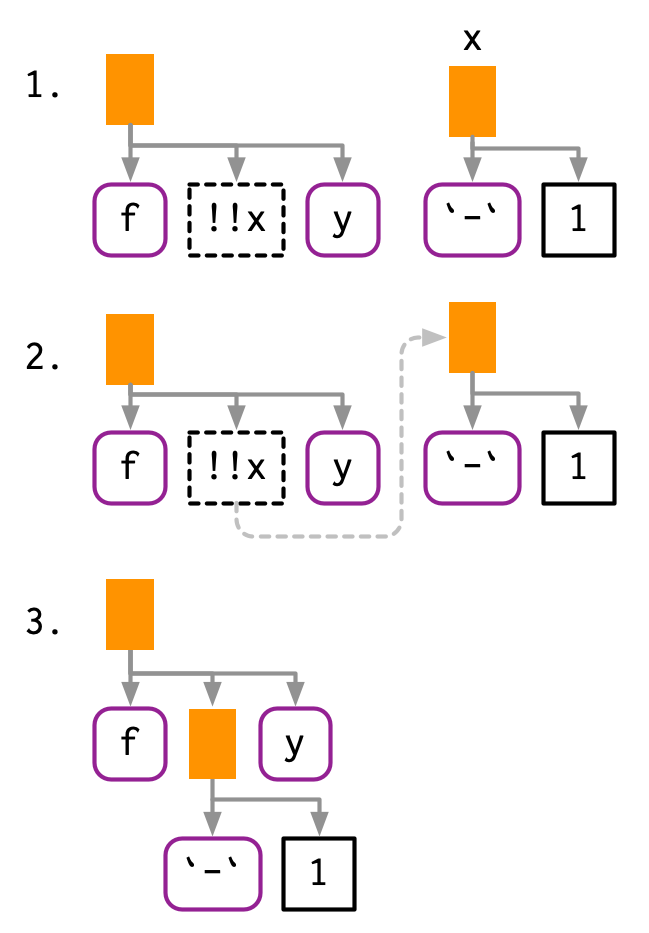
\includegraphics[width=2.7in]{diagrams/quotation/bang-bang} \end{center}

As well as call objects, \texttt{!!} also works with symbols and constants:

\begin{Shaded}
\begin{Highlighting}[]
\NormalTok{a <-}\StringTok{ }\KeywordTok{sym}\NormalTok{(}\StringTok{"y"}\NormalTok{)}
\NormalTok{b <-}\StringTok{ }\DecValTok{1}
\KeywordTok{expr}\NormalTok{(}\KeywordTok{f}\NormalTok{(}\OperatorTok{!!}\NormalTok{a, }\OperatorTok{!!}\NormalTok{b))}
\CommentTok{#> f(y, 1)}
\end{Highlighting}
\end{Shaded}

\begin{center}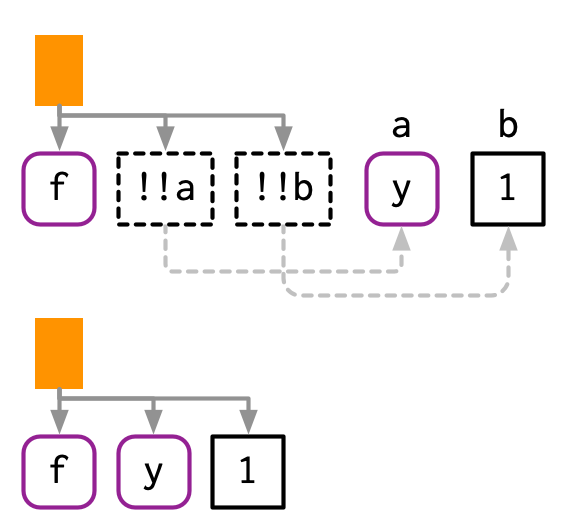
\includegraphics[width=2.36in]{diagrams/quotation/simple} \end{center}

If the right-hand side of \texttt{!!} is a function call, \texttt{!!} will evaluate it and insert the results:

\begin{Shaded}
\begin{Highlighting}[]
\NormalTok{mean_rm <-}\StringTok{ }\ControlFlowTok{function}\NormalTok{(var) \{}
\NormalTok{  var <-}\StringTok{ }\KeywordTok{ensym}\NormalTok{(var)}
  \KeywordTok{expr}\NormalTok{(}\KeywordTok{mean}\NormalTok{(}\OperatorTok{!!}\NormalTok{var, }\DataTypeTok{na.rm =} \OtherTok{TRUE}\NormalTok{))}
\NormalTok{\}}
\KeywordTok{expr}\NormalTok{(}\OperatorTok{!!}\KeywordTok{mean_rm}\NormalTok{(x) }\OperatorTok{+}\StringTok{ }\OperatorTok{!!}\KeywordTok{mean_rm}\NormalTok{(y))}
\CommentTok{#> mean(x, na.rm = TRUE) + mean(y, na.rm = TRUE)}
\end{Highlighting}
\end{Shaded}

\texttt{!!} preserves operator precedence because it works with expressions.

\begin{Shaded}
\begin{Highlighting}[]
\NormalTok{x1 <-}\StringTok{ }\KeywordTok{expr}\NormalTok{(x }\OperatorTok{+}\StringTok{ }\DecValTok{1}\NormalTok{)}
\NormalTok{x2 <-}\StringTok{ }\KeywordTok{expr}\NormalTok{(x }\OperatorTok{+}\StringTok{ }\DecValTok{2}\NormalTok{)}

\KeywordTok{expr}\NormalTok{(}\OperatorTok{!!}\NormalTok{x1 }\OperatorTok{/}\StringTok{ }\OperatorTok{!!}\NormalTok{x2)}
\CommentTok{#> (x + 1)/(x + 2)}
\end{Highlighting}
\end{Shaded}

\begin{center}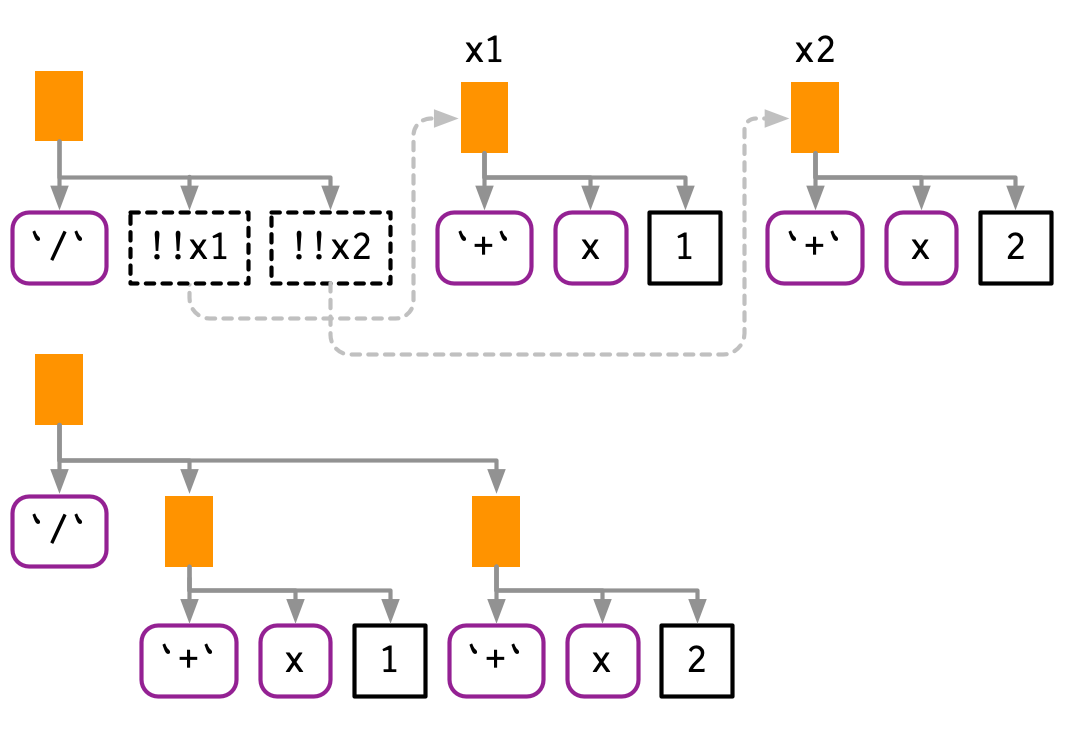
\includegraphics[width=4.47in]{diagrams/quotation/infix} \end{center}

If we simply pasted the text of the expressions together, we'd end up with \texttt{x\ +\ 1\ /\ x\ +\ 2}, which has a very different AST:

\begin{center}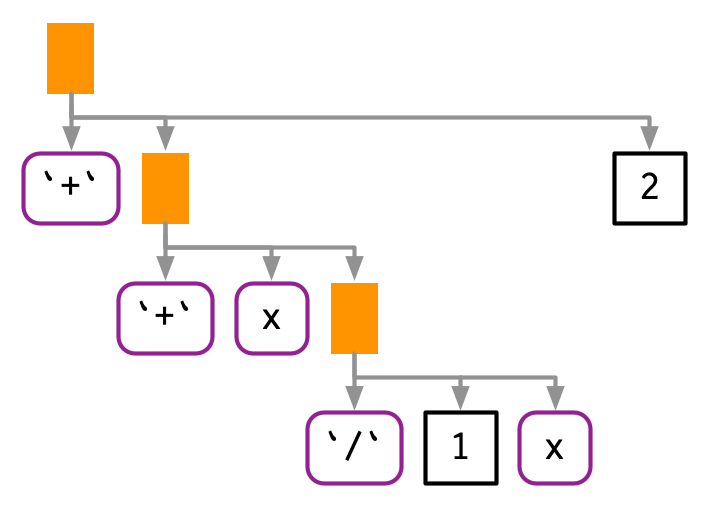
\includegraphics[width=2.95in]{diagrams/quotation/infix-bad} \end{center}

\hypertarget{unquoting-a-function}{%
\subsection{Unquoting a function}\label{unquoting-a-function}}

\index{unquoting!functions}

\texttt{!!} is most commonly used to replace the arguments to a function, but you can also use it to replace the function itself. The only challenge here is operator precedence: \texttt{expr(!!f(x,\ y))} unquotes the result of \texttt{f(x,\ y)}, so you need an extra pair of parentheses.

\begin{Shaded}
\begin{Highlighting}[]
\NormalTok{f <-}\StringTok{ }\KeywordTok{expr}\NormalTok{(foo)}
\KeywordTok{expr}\NormalTok{((}\OperatorTok{!!}\NormalTok{f)(x, y))}
\CommentTok{#> foo(x, y)}
\end{Highlighting}
\end{Shaded}

This also works when \texttt{f} is itself a call:

\begin{Shaded}
\begin{Highlighting}[]
\NormalTok{f <-}\StringTok{ }\KeywordTok{expr}\NormalTok{(pkg}\OperatorTok{::}\NormalTok{foo)}
\KeywordTok{expr}\NormalTok{((}\OperatorTok{!!}\NormalTok{f)(x, y))}
\CommentTok{#> pkg::foo(x, y)}
\end{Highlighting}
\end{Shaded}

\begin{center}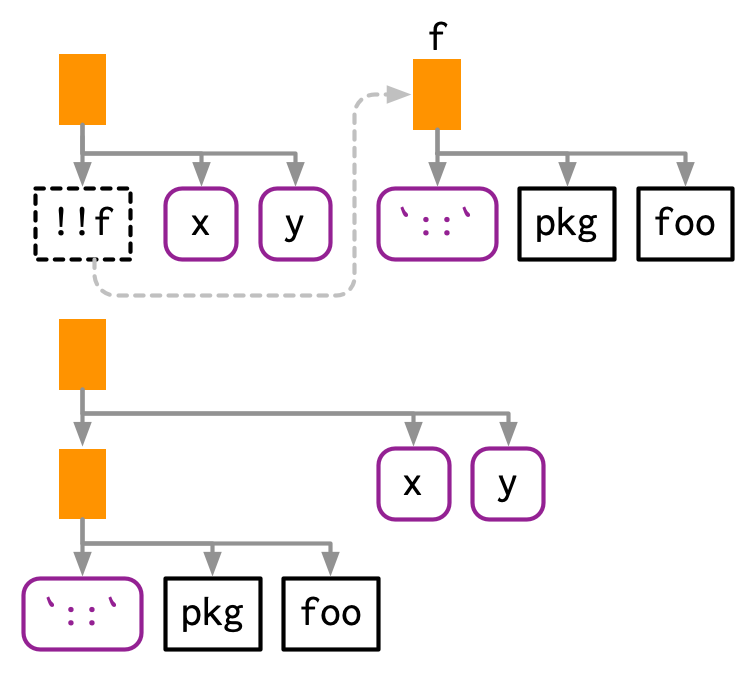
\includegraphics[width=3.1in]{diagrams/quotation/fun} \end{center}

Because of the large number of parentheses involved, it can be clearer to use \texttt{rlang::call2()}:

\begin{Shaded}
\begin{Highlighting}[]
\NormalTok{f <-}\StringTok{ }\KeywordTok{expr}\NormalTok{(pkg}\OperatorTok{::}\NormalTok{foo)}
\KeywordTok{call2}\NormalTok{(f, }\KeywordTok{expr}\NormalTok{(x), }\KeywordTok{expr}\NormalTok{(y))}
\CommentTok{#> pkg::foo(x, y)}
\end{Highlighting}
\end{Shaded}

\hypertarget{unquote-missing}{%
\subsection{Unquoting a missing argument}\label{unquote-missing}}

\index{unquoting!missing arguments}
\index{missing arguments!unquoting}

Very occasionally it is useful to unquote a missing argument (Section \ref{empty-symbol}), but the naive approach doesn't work:

\begin{Shaded}
\begin{Highlighting}[]
\NormalTok{arg <-}\StringTok{ }\KeywordTok{missing_arg}\NormalTok{()}
\KeywordTok{expr}\NormalTok{(}\KeywordTok{foo}\NormalTok{(}\OperatorTok{!!}\NormalTok{arg, }\OperatorTok{!!}\NormalTok{arg))}
\CommentTok{#> Error in enexpr(expr): argument "arg" is missing, with no default}
\end{Highlighting}
\end{Shaded}

You can work around this with the \texttt{rlang::maybe\_missing()} helper:

\begin{Shaded}
\begin{Highlighting}[]
\KeywordTok{expr}\NormalTok{(}\KeywordTok{foo}\NormalTok{(}\OperatorTok{!!}\KeywordTok{maybe_missing}\NormalTok{(arg), }\OperatorTok{!!}\KeywordTok{maybe_missing}\NormalTok{(arg)))}
\CommentTok{#> foo(, )}
\end{Highlighting}
\end{Shaded}

\hypertarget{unquoting-in-special-forms}{%
\subsection{Unquoting in special forms}\label{unquoting-in-special-forms}}

\index{unquoting!special forms}
\index{special forms!unquoting}

There are a few special forms where unquoting is a syntax error. Take \texttt{\$} for example: it must always be followed by the name of a variable, not another expression. This means attempting to unquote with \texttt{\$} will fail with a syntax error:

\begin{Shaded}
\begin{Highlighting}[]
\KeywordTok{expr}\NormalTok{(df}\OperatorTok{$!!}\NormalTok{x)}
\CommentTok{#> Error: unexpected '!' in "expr(df$!"}
\end{Highlighting}
\end{Shaded}

To make unquoting work, you'll need to use the prefix form (Section \ref{prefix-transform}):

\begin{Shaded}
\begin{Highlighting}[]
\NormalTok{x <-}\StringTok{ }\KeywordTok{expr}\NormalTok{(x)}
\KeywordTok{expr}\NormalTok{(}\StringTok{`}\DataTypeTok{$}\StringTok{`}\NormalTok{(df, }\OperatorTok{!!}\NormalTok{x))}
\CommentTok{#> df$x}
\end{Highlighting}
\end{Shaded}

\hypertarget{unquoting-many-arguments}{%
\subsection{Unquoting many arguments}\label{unquoting-many-arguments}}

\indexc{"!"!"!}

\index{splicing!expressions}
\index{splicing|seealso {"!"!"!}}
\index{unquoting!many arguments}

\texttt{!!} is a one-to-one replacement. \texttt{!!!} (called ``unquote-splice'', and pronounced bang-bang-bang) is a one-to-many replacement. It takes a list of expressions and inserts them at the location of the \texttt{!!!}:

\begin{Shaded}
\begin{Highlighting}[]
\NormalTok{xs <-}\StringTok{ }\KeywordTok{exprs}\NormalTok{(}\DecValTok{1}\NormalTok{, a, }\OperatorTok{-}\NormalTok{b)}
\KeywordTok{expr}\NormalTok{(}\KeywordTok{f}\NormalTok{(}\OperatorTok{!!!}\NormalTok{xs, y))}
\CommentTok{#> f(1, a, -b, y)}

\CommentTok{# Or with names}
\NormalTok{ys <-}\StringTok{ }\KeywordTok{set_names}\NormalTok{(xs, }\KeywordTok{c}\NormalTok{(}\StringTok{"a"}\NormalTok{, }\StringTok{"b"}\NormalTok{, }\StringTok{"c"}\NormalTok{))}
\KeywordTok{expr}\NormalTok{(}\KeywordTok{f}\NormalTok{(}\OperatorTok{!!!}\NormalTok{ys, }\DataTypeTok{d =} \DecValTok{4}\NormalTok{))}
\CommentTok{#> f(a = 1, b = a, c = -b, d = 4)}
\end{Highlighting}
\end{Shaded}

\begin{center}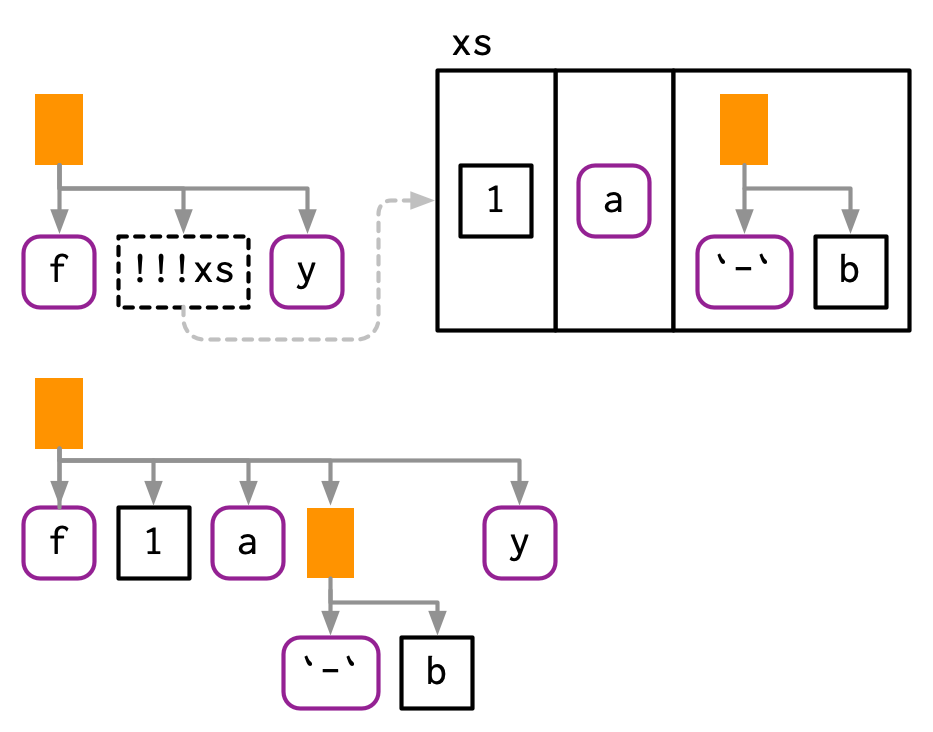
\includegraphics[width=3.89in]{diagrams/quotation/bang-bang-bang} \end{center}

\texttt{!!!} can be used in any rlang function that takes \texttt{...} regardless of whether or not \texttt{...} is quoted or evaluated. We'll come back to this in Section \ref{tidy-dots}; for now note that this can be useful in \texttt{call2()}.

\begin{Shaded}
\begin{Highlighting}[]
\KeywordTok{call2}\NormalTok{(}\StringTok{"f"}\NormalTok{, }\OperatorTok{!!!}\NormalTok{xs, }\KeywordTok{expr}\NormalTok{(y))}
\CommentTok{#> f(1, a, -b, y)}
\end{Highlighting}
\end{Shaded}

\hypertarget{the-polite-fiction-of}{%
\subsection{\texorpdfstring{The polite fiction of \texttt{!!}}{The polite fiction of !!}}\label{the-polite-fiction-of}}

So far we have acted as if \texttt{!!} and \texttt{!!!} are regular prefix operators like \texttt{+} , \texttt{-}, and \texttt{!}. They're not. From R's perspective, \texttt{!!} and \texttt{!!!} are simply the repeated application of \texttt{!}:

\begin{Shaded}
\begin{Highlighting}[]
\OperatorTok{!!}\OtherTok{TRUE}
\CommentTok{#> [1] TRUE}
\OperatorTok{!!!}\OtherTok{TRUE}
\CommentTok{#> [1] FALSE}
\end{Highlighting}
\end{Shaded}

\texttt{!!} and \texttt{!!!} behave specially inside all quoting functions powered by rlang, where they behave like real operators with precedence equivalent to unary \texttt{+} and \texttt{-}. This requires considerable work inside rlang, but means that you can write \texttt{!!x\ +\ !!y} instead of \texttt{(!!x)\ +\ (!!y)}.

The biggest downside\footnote{Prior to R 3.5.1, there was another major downside: the R deparser treated \texttt{!!x} as \texttt{!(!x)}. This is why in old versions of R you might see extra parentheses when printing expressions. The good news is that these parentheses are not real and can be safely ignored most of the time. The bad news is that they will become real if you reparse that printed output to R code. These roundtripped functions will not work as expected since \texttt{!(!x)} does not unquote.} to using a fake operator is that you might get silent errors when misusing \texttt{!!} outside of quasiquoting functions. Most of the time this is not an issue because \texttt{!!} is typically used to unquote expressions or quosures. Since expressions are not supported by the negation operator, you will get an argument type error in this case:

\begin{Shaded}
\begin{Highlighting}[]
\NormalTok{x <-}\StringTok{ }\KeywordTok{quote}\NormalTok{(variable)}
\OperatorTok{!!}\NormalTok{x}
\CommentTok{#> Error in !x: invalid argument type}
\end{Highlighting}
\end{Shaded}

But you can get silently incorrect results when working with numeric values:

\begin{Shaded}
\begin{Highlighting}[]
\NormalTok{df <-}\StringTok{ }\KeywordTok{data.frame}\NormalTok{(}\DataTypeTok{x =} \DecValTok{1}\OperatorTok{:}\DecValTok{5}\NormalTok{)}
\NormalTok{y <-}\StringTok{ }\DecValTok{100}
\KeywordTok{with}\NormalTok{(df, x }\OperatorTok{+}\StringTok{ }\OperatorTok{!!}\NormalTok{y)}
\CommentTok{#> [1] 2 3 4 5 6}
\end{Highlighting}
\end{Shaded}

Given these drawbacks, you might wonder why we introduced new syntax instead of using regular function calls. Indeed, early versions of tidy evaluation used function calls like \texttt{UQ()} and \texttt{UQS()}. However, they're not really function calls, and pretending they are leads to a misleading mental mode. We chose \texttt{!!} and \texttt{!!!} as the least-bad solution:

\begin{itemize}
\item
  The are visually strong and don't look like existing syntax. When you
  see \texttt{!!x} or \texttt{!!!x} it's clear that something unusual is happening.
\item
  They overrides a rarely used piece of syntax, as double negation is not a
  common pattern in R\footnote{Unlike, say, javascript, where \texttt{!!x} is a commonly used shortcut to convert an integer into a logical.}. If you you do need it, you can just
  add parentheses \texttt{!(!x)}.
\end{itemize}

\hypertarget{non-standard-ast}{%
\subsection{Non-standard ASTs}\label{non-standard-ast}}

\index{ASTs!non-standard}

With unquoting, it's easy to create non-standard ASTs, i.e.~ASTs that contain components that are not expressions. (It is also possible to create non-standard ASTs by directly manipulating the underlying objects, but it's harder to do so accidentally.) These are valid, and occasionally useful, but their correct use is beyond the scope of this book. However, it's important to learn about them, because they can be deparsed, and hence printed, in misleading ways.

For example, if you inline more complex objects, their attributes are not printed. This can lead to confusing output:

\begin{Shaded}
\begin{Highlighting}[]
\NormalTok{x1 <-}\StringTok{ }\KeywordTok{expr}\NormalTok{(}\KeywordTok{class}\NormalTok{(}\OperatorTok{!!}\KeywordTok{data.frame}\NormalTok{(}\DataTypeTok{x =} \DecValTok{10}\NormalTok{)))}
\NormalTok{x1}
\CommentTok{#> class(list(x = 10))}
\KeywordTok{eval}\NormalTok{(x1)}
\CommentTok{#> [1] "data.frame"}
\end{Highlighting}
\end{Shaded}

You have two main tools to reduce this confusion: \texttt{rlang::expr\_print()} and \texttt{lobstr::ast()}:

\begin{Shaded}
\begin{Highlighting}[]
\KeywordTok{expr_print}\NormalTok{(x1)}
\CommentTok{#> class(<data.frame>)}
\NormalTok{lobstr}\OperatorTok{::}\KeywordTok{ast}\NormalTok{(}\OperatorTok{!!}\NormalTok{x1)}
\CommentTok{#> █─class }
\CommentTok{#> └─<inline data.frame>}
\end{Highlighting}
\end{Shaded}

Another confusing case arises if you inline an integer sequence:

\begin{Shaded}
\begin{Highlighting}[]
\NormalTok{x2 <-}\StringTok{ }\KeywordTok{expr}\NormalTok{(}\KeywordTok{f}\NormalTok{(}\OperatorTok{!!}\KeywordTok{c}\NormalTok{(1L, 2L, 3L, 4L, 5L)))}
\NormalTok{x2}
\CommentTok{#> f(1:5)}
\KeywordTok{expr_print}\NormalTok{(x2)}
\CommentTok{#> f(<int: 1L, 2L, 3L, 4L, 5L>)}
\NormalTok{lobstr}\OperatorTok{::}\KeywordTok{ast}\NormalTok{(}\OperatorTok{!!}\NormalTok{x2)}
\CommentTok{#> █─f }
\CommentTok{#> └─<inline integer>}
\end{Highlighting}
\end{Shaded}

It's also possible to create regular ASTs that can not be generated from code because of operator precedence. In this case, R will print parentheses that do not exist in the AST:

\begin{Shaded}
\begin{Highlighting}[]
\NormalTok{x3 <-}\StringTok{ }\KeywordTok{expr}\NormalTok{(}\DecValTok{1} \OperatorTok{+}\StringTok{ }\OperatorTok{!!}\KeywordTok{expr}\NormalTok{(}\DecValTok{2} \OperatorTok{+}\StringTok{ }\DecValTok{3}\NormalTok{))}
\NormalTok{x3}
\CommentTok{#> 1 + (2 + 3)}

\NormalTok{lobstr}\OperatorTok{::}\KeywordTok{ast}\NormalTok{(}\OperatorTok{!!}\NormalTok{x3)}
\CommentTok{#> █─`+` }
\CommentTok{#> ├─1 }
\CommentTok{#> └─█─`+` }
\CommentTok{#>   ├─2 }
\CommentTok{#>   └─3}
\end{Highlighting}
\end{Shaded}

\hypertarget{exercises-6}{%
\subsection{Exercises}\label{exercises-6}}

\begin{enumerate}
\def\labelenumi{\arabic{enumi}.}
\item
  Given the following components:

\begin{Shaded}
\begin{Highlighting}[]
\NormalTok{xy <-}\StringTok{ }\KeywordTok{expr}\NormalTok{(x }\OperatorTok{+}\StringTok{ }\NormalTok{y)}
\NormalTok{xz <-}\StringTok{ }\KeywordTok{expr}\NormalTok{(x }\OperatorTok{+}\StringTok{ }\NormalTok{z)}
\NormalTok{yz <-}\StringTok{ }\KeywordTok{expr}\NormalTok{(y }\OperatorTok{+}\StringTok{ }\NormalTok{z)}
\NormalTok{abc <-}\StringTok{ }\KeywordTok{exprs}\NormalTok{(a, b, c)}
\end{Highlighting}
\end{Shaded}

  Use quasiquotation to construct the following calls:

\begin{Shaded}
\begin{Highlighting}[]
\NormalTok{(x }\OperatorTok{+}\StringTok{ }\NormalTok{y) }\OperatorTok{/}\StringTok{ }\NormalTok{(y }\OperatorTok{+}\StringTok{ }\NormalTok{z)}
\OperatorTok{-}\NormalTok{(x }\OperatorTok{+}\StringTok{ }\NormalTok{z) }\OperatorTok{^}\StringTok{ }\NormalTok{(y }\OperatorTok{+}\StringTok{ }\NormalTok{z)}
\NormalTok{(x }\OperatorTok{+}\StringTok{ }\NormalTok{y) }\OperatorTok{+}\StringTok{ }\NormalTok{(y }\OperatorTok{+}\StringTok{ }\NormalTok{z) }\OperatorTok{-}\StringTok{ }\NormalTok{(x }\OperatorTok{+}\StringTok{ }\NormalTok{y)}
\KeywordTok{atan2}\NormalTok{(x }\OperatorTok{+}\StringTok{ }\NormalTok{y, y }\OperatorTok{+}\StringTok{ }\NormalTok{z)}
\KeywordTok{sum}\NormalTok{(x }\OperatorTok{+}\StringTok{ }\NormalTok{y, x }\OperatorTok{+}\StringTok{ }\NormalTok{y, y }\OperatorTok{+}\StringTok{ }\NormalTok{z)}
\KeywordTok{sum}\NormalTok{(a, b, c)}
\KeywordTok{mean}\NormalTok{(}\KeywordTok{c}\NormalTok{(a, b, c), }\DataTypeTok{na.rm =} \OtherTok{TRUE}\NormalTok{)}
\KeywordTok{foo}\NormalTok{(}\DataTypeTok{a =}\NormalTok{ x }\OperatorTok{+}\StringTok{ }\NormalTok{y, }\DataTypeTok{b =}\NormalTok{ y }\OperatorTok{+}\StringTok{ }\NormalTok{z)}
\end{Highlighting}
\end{Shaded}
\item
  The following two calls print the same, but are actually different:

\begin{Shaded}
\begin{Highlighting}[]
\NormalTok{(a <-}\StringTok{ }\KeywordTok{expr}\NormalTok{(}\KeywordTok{mean}\NormalTok{(}\DecValTok{1}\OperatorTok{:}\DecValTok{10}\NormalTok{)))}
\CommentTok{#> mean(1:10)}
\NormalTok{(b <-}\StringTok{ }\KeywordTok{expr}\NormalTok{(}\KeywordTok{mean}\NormalTok{(}\OperatorTok{!!}\NormalTok{(}\DecValTok{1}\OperatorTok{:}\DecValTok{10}\NormalTok{))))}
\CommentTok{#> mean(1:10)}
\KeywordTok{identical}\NormalTok{(a, b)}
\CommentTok{#> [1] FALSE}
\end{Highlighting}
\end{Shaded}

  What's the difference? Which one is more natural?
\end{enumerate}

\hypertarget{base-nonquote}{%
\section{Non-quoting}\label{base-nonquote}}

\indexc{bquote()}

\index{unquoting!base R}

Base R has one function that implements quasiquotation: \texttt{bquote()}. It uses \texttt{.()} for unquoting:

\begin{Shaded}
\begin{Highlighting}[]
\NormalTok{xyz <-}\StringTok{ }\KeywordTok{bquote}\NormalTok{((x }\OperatorTok{+}\StringTok{ }\NormalTok{y }\OperatorTok{+}\StringTok{ }\NormalTok{z))}
\KeywordTok{bquote}\NormalTok{(}\OperatorTok{-}\NormalTok{.(xyz) }\OperatorTok{/}\StringTok{ }\DecValTok{2}\NormalTok{)}
\CommentTok{#> -(x + y + z)/2}
\end{Highlighting}
\end{Shaded}

\texttt{bquote()} isn't used by any other function in base R, and has had relatively little impact on how R code is written. There are three challenges to effective use of \texttt{bquote()}:

\begin{itemize}
\item
  It is only easily used with your code; it is hard to apply it to arbitrary
  code supplied by a user.
\item
  It does not provide an unquote-splice operator that allows you to unquote
  multiple expressions stored in a list.
\item
  It lacks the ability to handle code accompanied by an environment, which
  is crucial for functions that evaluate code in the context of a data frame,
  like \texttt{subset()} and friends.
\end{itemize}

Instead functions that quote an argument use some other technique to allow indirect specification. Rather than using use unquoting all base R approaches selectively turn quoting off, so I call them \textbf{non-quoting} techniques.

There are four basic forms seen in base R:

\begin{itemize}
\item
  A pair of quoting and non-quoting functions. For example, \texttt{\$} has two
  arguments, and the second argument is quoted. This is easier to see if you
  write in prefix form: \texttt{mtcars\$cyl} is equivalent to \texttt{\textasciigrave{}\$\textasciigrave{}(mtcars,\ cyl)}.
  If you want to refer to a variable indirectly, you use \texttt{{[}{[}}, as it
  takes the name of a variable as a string.

\begin{Shaded}
\begin{Highlighting}[]
\NormalTok{x <-}\StringTok{ }\KeywordTok{list}\NormalTok{(}\DataTypeTok{var =} \DecValTok{1}\NormalTok{, }\DataTypeTok{y =} \DecValTok{2}\NormalTok{)}
\NormalTok{var <-}\StringTok{ "y"}

\NormalTok{x}\OperatorTok{$}\NormalTok{var}
\CommentTok{#> [1] 1}
\NormalTok{x[[var]]}
\CommentTok{#> [1] 2}
\end{Highlighting}
\end{Shaded}

  There are three other quoting functions closely related to \texttt{\$}: \texttt{subset()},
  \texttt{transform()}, and \texttt{with()}. These are seen as wrappers around \texttt{\$} only
  suitable for interactive use so they all have the same non-quoting
  alternative: \texttt{{[}}

  \texttt{\textless{}-}/\texttt{assign()} and \texttt{::}/\texttt{getExportedValue()} work similarly to \texttt{\$}/\texttt{{[}}.
  \indexc{\$}
  \indexc{<-}
\item
  A pair of quoting and non-quoting arguments. For example, \texttt{rm()} allows
  you to provide bare variable names in \texttt{...}, or a character vector of
  variable names in \texttt{list}:

\begin{Shaded}
\begin{Highlighting}[]
\NormalTok{x <-}\StringTok{ }\DecValTok{1}
\KeywordTok{rm}\NormalTok{(x)}

\NormalTok{y <-}\StringTok{ }\DecValTok{2}
\NormalTok{vars <-}\StringTok{ }\KeywordTok{c}\NormalTok{(}\StringTok{"y"}\NormalTok{, }\StringTok{"vars"}\NormalTok{)}
\KeywordTok{rm}\NormalTok{(}\DataTypeTok{list =}\NormalTok{ vars)}
\end{Highlighting}
\end{Shaded}

  \texttt{data()} and \texttt{save()} work similarly.
  \indexc{rm()}
\item
  An argument that controls whether a different argument is quoting or
  non-quoting. For example, in \texttt{library()}, the \texttt{character.only} argument
  controls the quoting behaviour of the first argument, \texttt{package}:

\begin{Shaded}
\begin{Highlighting}[]
\KeywordTok{library}\NormalTok{(MASS)}

\NormalTok{pkg <-}\StringTok{ "MASS"}
\KeywordTok{library}\NormalTok{(pkg, }\DataTypeTok{character.only =} \OtherTok{TRUE}\NormalTok{)}
\end{Highlighting}
\end{Shaded}

  \texttt{demo()}, \texttt{detach()}, \texttt{example()}, and \texttt{require()} work similarly.
  \indexc{library()}
\item
  Quoting if evaluation fails. For example, the first argument to \texttt{help()}
  is non-quoting if it evaluates to a string; if evaluation fails, the
  first argument is quoted.

\begin{Shaded}
\begin{Highlighting}[]
\CommentTok{# Shows help for var}
\KeywordTok{help}\NormalTok{(var)}

\NormalTok{var <-}\StringTok{ "mean"}
\CommentTok{# Shows help for mean}
\KeywordTok{help}\NormalTok{(var)}

\NormalTok{var <-}\StringTok{ }\DecValTok{10}
\CommentTok{# Shows help for var}
\KeywordTok{help}\NormalTok{(var)}
\end{Highlighting}
\end{Shaded}

  \texttt{ls()}, \texttt{page()}, and \texttt{match.fun()} work similarly.
  \indexc{help()}
\end{itemize}

\indexc{lm()}

Another important class of quoting functions are the base modelling and plotting functions, which follow the so-called standard non-standard evaluation rules: \url{http://developer.r-project.org/nonstandard-eval.pdf}. For example, \texttt{lm()} quotes the \texttt{weight} and \texttt{subset} arguments, and when used with a formula argument, the plotting function quotes the aesthetic arguments (\texttt{col}, \texttt{cex}, etc):

\begin{Shaded}
\begin{Highlighting}[]
\KeywordTok{palette}\NormalTok{(RColorBrewer}\OperatorTok{::}\KeywordTok{brewer.pal}\NormalTok{(}\DecValTok{3}\NormalTok{, }\StringTok{"Set1"}\NormalTok{))}
\KeywordTok{plot}\NormalTok{(}
\NormalTok{  Sepal.Length }\OperatorTok{~}\StringTok{ }\NormalTok{Petal.Length, }
  \DataTypeTok{data =}\NormalTok{ iris, }
  \DataTypeTok{col =}\NormalTok{ Species, }
  \DataTypeTok{pch =} \DecValTok{20}\NormalTok{, }
  \DataTypeTok{cex =} \DecValTok{2}
\NormalTok{)}
\end{Highlighting}
\end{Shaded}

\begin{center}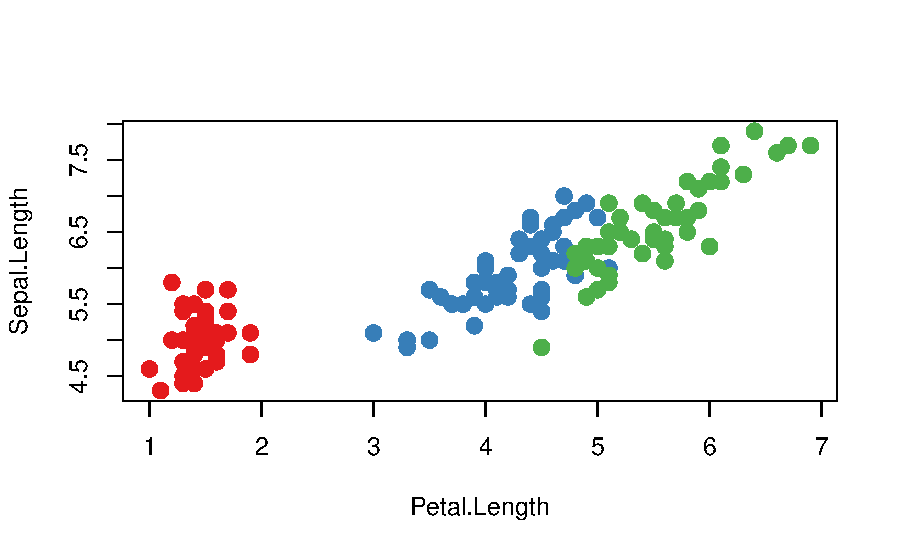
\includegraphics[width=0.7\linewidth]{Quotation_files/figure-latex/unnamed-chunk-58-1} \end{center}

These functions have no built-in options for indirect specification, but you'll learn how to simulate unquoting in Section \ref{base-nonquote}.

\hypertarget{tidy-dots}{%
\section{\texorpdfstring{Dot-dot-dot (\texttt{...})}{Dot-dot-dot (...)}}\label{tidy-dots}}

\indexc{...}

\index{tidy dots}

\texttt{!!!} is useful because it's not uncommon to have a list of expressions that you want to insert into a call. It turns out that this pattern is common elsewhere. Take the following two motivating problems:

\begin{itemize}
\item
  What do you do if the elements you want to put in \texttt{...} are already stored
  in a list? For example, imagine you have a list of data frames that
  you want to \texttt{rbind()} together:

\begin{Shaded}
\begin{Highlighting}[]
\NormalTok{dfs <-}\StringTok{ }\KeywordTok{list}\NormalTok{(}
  \DataTypeTok{a =} \KeywordTok{data.frame}\NormalTok{(}\DataTypeTok{x =} \DecValTok{1}\NormalTok{, }\DataTypeTok{y =} \DecValTok{2}\NormalTok{),}
  \DataTypeTok{b =} \KeywordTok{data.frame}\NormalTok{(}\DataTypeTok{x =} \DecValTok{3}\NormalTok{, }\DataTypeTok{y =} \DecValTok{4}\NormalTok{)}
\NormalTok{)}
\end{Highlighting}
\end{Shaded}

  You could solve this specific case with \texttt{rbind(dfs\$a,\ dfs\$b)}, but how
  do you generalise that solution to a list of arbitrary length?
\item
  What do you do if you want to supply the argument name indirectly? For
  example, imagine you want to create a single column data frame where
  the name of the column is specified in a variable:

\begin{Shaded}
\begin{Highlighting}[]
\NormalTok{var <-}\StringTok{ "x"}
\NormalTok{val <-}\StringTok{ }\KeywordTok{c}\NormalTok{(}\DecValTok{4}\NormalTok{, }\DecValTok{3}\NormalTok{, }\DecValTok{9}\NormalTok{)}
\end{Highlighting}
\end{Shaded}

  In this case, you could create a data frame and then change names
  (i.e. \texttt{setNames(data.frame(val),\ var)}), but this feels inelegant.
  How can we do better?
\end{itemize}

One way to think about these problems is to draw explicit parallels to quasiquotation:

\begin{itemize}
\item
  Row-binding multiple data frames is like unquote-splicing: we want to inline
  individual elements of the list into the call:

\begin{Shaded}
\begin{Highlighting}[]
\NormalTok{dplyr}\OperatorTok{::}\KeywordTok{bind_rows}\NormalTok{(}\OperatorTok{!!!}\NormalTok{dfs)}
\CommentTok{#>   x y}
\CommentTok{#> 1 1 2}
\CommentTok{#> 2 3 4}
\end{Highlighting}
\end{Shaded}

  When used in this context, the behaviour of \texttt{!!!} is known as ``spatting'' in
  Ruby, Go, PHP, and Julia. It is closely related to \texttt{*args} (star-args) and
  \texttt{**kwarg} (star-star-kwargs) in Python, which are sometimes called argument
  unpacking.
  \index{splicing}
\item
  The second problem is like unquoting the left-hand side of \texttt{=}: rather
  than interpreting \texttt{var} literally, we want to use the value stored in the
  variable called \texttt{var}:

\begin{Shaded}
\begin{Highlighting}[]
\NormalTok{tibble}\OperatorTok{::}\KeywordTok{tibble}\NormalTok{(}\OperatorTok{!!}\NormalTok{var }\OperatorTok{:}\ErrorTok{=}\StringTok{ }\NormalTok{val)}
\CommentTok{#> # A tibble: 3 x 1}
\CommentTok{#>       x}
\CommentTok{#>   <dbl>}
\CommentTok{#> 1     4}
\CommentTok{#> 2     3}
\CommentTok{#> 3     9}
\end{Highlighting}
\end{Shaded}

  Note the use of \texttt{:=} (pronounced colon-equals) rather than \texttt{=}. Unfortunately
  we need this new operation because R's grammar does not allow expressions as
  argument names:

\begin{Shaded}
\begin{Highlighting}[]
\NormalTok{tibble}\OperatorTok{::}\KeywordTok{tibble}\NormalTok{(}\OperatorTok{!!}\DataTypeTok{var =}\NormalTok{ value)}
\CommentTok{#> Error: unexpected '=' in "tibble::tibble(!!var ="}
\end{Highlighting}
\end{Shaded}

  \texttt{:=} is like a vestigial organ: it's recognised by R's parser, but it
  doesn't have any code associated with it. It looks like an \texttt{=} but allows
  expressions on either side, making it a more flexible alternative to \texttt{=}.
  It is used in data.table for similar reasons.
  \indexc{:=}
\end{itemize}

Base R takes a different approach, which we'll come back to Section @ref\{do-call\}.

We say functions that support these tools, without quoting arguments, have \textbf{tidy dots}\footnote{This is admittedly not the most creative of names, but it clearly suggests it's something that has been added to R after the fact.}. To gain tidy dots behaviour in your own function, all you need to do is use \texttt{list2()}.

\hypertarget{examples}{%
\subsection{Examples}\label{examples}}

\index{attributes!attributes@\texttt{attributes()}}

One place we could use \texttt{list2()} is to create a wrapper around \texttt{attributes()} that allows us to set attributes flexibly:

\begin{Shaded}
\begin{Highlighting}[]
\NormalTok{set_attr <-}\StringTok{ }\ControlFlowTok{function}\NormalTok{(.x, ...) \{}
\NormalTok{  attr <-}\StringTok{ }\NormalTok{rlang}\OperatorTok{::}\KeywordTok{list2}\NormalTok{(...)}
  \KeywordTok{attributes}\NormalTok{(.x) <-}\StringTok{ }\NormalTok{attr}
\NormalTok{  .x}
\NormalTok{\}}

\NormalTok{attrs <-}\StringTok{ }\KeywordTok{list}\NormalTok{(}\DataTypeTok{x =} \DecValTok{1}\NormalTok{, }\DataTypeTok{y =} \DecValTok{2}\NormalTok{)}
\NormalTok{attr_name <-}\StringTok{ "z"}

\DecValTok{1}\OperatorTok{:}\DecValTok{10} \OperatorTok
\StringTok{  }\KeywordTok{set_attr}\NormalTok{(}\DataTypeTok{w =} \DecValTok{0}\NormalTok{, }\OperatorTok{!!!}\NormalTok{attrs, }\OperatorTok{!!}\NormalTok{attr_name }\OperatorTok{:}\ErrorTok{=}\StringTok{ }\DecValTok{3}\NormalTok{) }\OperatorTok\StringTok{ }
\StringTok{  }\KeywordTok{str}\NormalTok{()}
\CommentTok{#>  int [1:10] 1 2 3 4 5 6 7 8 9 10}
\CommentTok{#>  - attr(*, "w")= num 0}
\CommentTok{#>  - attr(*, "x")= num 1}
\CommentTok{#>  - attr(*, "y")= num 2}
\CommentTok{#>  - attr(*, "z")= num 3}
\end{Highlighting}
\end{Shaded}

\hypertarget{exec}{%
\subsection{\texorpdfstring{\texttt{exec()}}{exec()}}\label{exec}}

\indexc{exec()}
\indexc{list2()}

What if you want to use this technique with a function that doesn't have tidy dots? One option is to use \texttt{rlang::exec()} to call a function with some arguments supplied directly (in \texttt{...}) and others indirectly (in a list):

\begin{Shaded}
\begin{Highlighting}[]
\CommentTok{# Directly}
\KeywordTok{exec}\NormalTok{(}\StringTok{"mean"}\NormalTok{, }\DataTypeTok{x =} \DecValTok{1}\OperatorTok{:}\DecValTok{10}\NormalTok{, }\DataTypeTok{na.rm =} \OtherTok{TRUE}\NormalTok{, }\DataTypeTok{trim =} \FloatTok{0.1}\NormalTok{)}
\CommentTok{#> [1] 5.5}

\CommentTok{# Indirectly}
\NormalTok{args <-}\StringTok{ }\KeywordTok{list}\NormalTok{(}\DataTypeTok{x =} \DecValTok{1}\OperatorTok{:}\DecValTok{10}\NormalTok{, }\DataTypeTok{na.rm =} \OtherTok{TRUE}\NormalTok{, }\DataTypeTok{trim =} \FloatTok{0.1}\NormalTok{)}
\KeywordTok{exec}\NormalTok{(}\StringTok{"mean"}\NormalTok{, }\OperatorTok{!!!}\NormalTok{args)}
\CommentTok{#> [1] 5.5}

\CommentTok{# Mixed}
\NormalTok{params <-}\StringTok{ }\KeywordTok{list}\NormalTok{(}\DataTypeTok{na.rm =} \OtherTok{TRUE}\NormalTok{, }\DataTypeTok{trim =} \FloatTok{0.1}\NormalTok{)}
\KeywordTok{exec}\NormalTok{(}\StringTok{"mean"}\NormalTok{, }\DataTypeTok{x =} \DecValTok{1}\OperatorTok{:}\DecValTok{10}\NormalTok{, }\OperatorTok{!!!}\NormalTok{params)}
\CommentTok{#> [1] 5.5}
\end{Highlighting}
\end{Shaded}

\texttt{rlang::exec()} also makes it possible to supply argument names indirectly:

\begin{Shaded}
\begin{Highlighting}[]
\NormalTok{arg_name <-}\StringTok{ "na.rm"}
\NormalTok{arg_val <-}\StringTok{ }\OtherTok{TRUE}
\KeywordTok{exec}\NormalTok{(}\StringTok{"mean"}\NormalTok{, }\DecValTok{1}\OperatorTok{:}\DecValTok{10}\NormalTok{, }\OperatorTok{!!}\NormalTok{arg_name }\OperatorTok{:}\ErrorTok{=}\StringTok{ }\NormalTok{arg_val)}
\CommentTok{#> [1] 5.5}
\end{Highlighting}
\end{Shaded}

And finally, it's useful if you have a vector of function names or a list of functions that you want to call with the same arguments:

\begin{Shaded}
\begin{Highlighting}[]
\NormalTok{x <-}\StringTok{ }\KeywordTok{c}\NormalTok{(}\KeywordTok{runif}\NormalTok{(}\DecValTok{10}\NormalTok{), }\OtherTok{NA}\NormalTok{)}
\NormalTok{funs <-}\StringTok{ }\KeywordTok{c}\NormalTok{(}\StringTok{"mean"}\NormalTok{, }\StringTok{"median"}\NormalTok{, }\StringTok{"sd"}\NormalTok{)}

\NormalTok{purrr}\OperatorTok{::}\KeywordTok{map_dbl}\NormalTok{(funs, exec, x, }\DataTypeTok{na.rm =} \OtherTok{TRUE}\NormalTok{)}
\CommentTok{#> [1] 0.444 0.482 0.298}
\end{Highlighting}
\end{Shaded}

\texttt{exec()} is closely related to \texttt{call2()}; where \texttt{call2()} returns an expression, \texttt{exec()} evaluates it.

\hypertarget{dots_list}{%
\subsection{\texorpdfstring{\texttt{dots\_list()}}{dots\_list()}}\label{dots_list}}

\indexc{dots\_list()}

\texttt{list2()} provides one other handy feature: by default it will ignore any empty arguments at the end. This is useful in functions like \texttt{tibble::tibble()} because it means that you can easily change the order of variables without worrying about the final comma:

\begin{Shaded}
\begin{Highlighting}[]
\CommentTok{# Can easily move x to first entry:}
\NormalTok{tibble}\OperatorTok{::}\KeywordTok{tibble}\NormalTok{(}
  \DataTypeTok{y =} \DecValTok{1}\OperatorTok{:}\DecValTok{5}\NormalTok{,}
  \DataTypeTok{z =} \DecValTok{3}\OperatorTok{:-}\DecValTok{1}\NormalTok{,}
  \DataTypeTok{x =} \DecValTok{5}\OperatorTok{:}\DecValTok{1}\NormalTok{,}
\NormalTok{)}

\CommentTok{# Need to remove comma from z and add comma to x}
\KeywordTok{data.frame}\NormalTok{(}
  \DataTypeTok{y =} \DecValTok{1}\OperatorTok{:}\DecValTok{5}\NormalTok{,}
  \DataTypeTok{z =} \DecValTok{3}\OperatorTok{:-}\DecValTok{1}\NormalTok{,}
  \DataTypeTok{x =} \DecValTok{5}\OperatorTok{:}\DecValTok{1}
\NormalTok{)}
\end{Highlighting}
\end{Shaded}

\texttt{list2()} is a wrapper around \texttt{rlang::dots\_list()} with defaults set to the most commonly used settings. You can get more control by calling \texttt{dots\_list()} directly:

\begin{itemize}
\item
  \texttt{.ignore\_empty} allows you to control exactly which arguments are ignored.
  The default ignores a single trailing argument to get the behaviour
  describe above, but you can choose to ignore all missing arguments, or
  no missing arguments.
\item
  \texttt{.homonoyms} controls what happens if multiple arguments use the same name:

\begin{Shaded}
\begin{Highlighting}[]
\KeywordTok{str}\NormalTok{(}\KeywordTok{dots_list}\NormalTok{(}\DataTypeTok{x =} \DecValTok{1}\NormalTok{, }\DataTypeTok{x =} \DecValTok{2}\NormalTok{))}
\CommentTok{#> List of 2}
\CommentTok{#>  $ x: num 1}
\CommentTok{#>  $ x: num 2}
\KeywordTok{str}\NormalTok{(}\KeywordTok{dots_list}\NormalTok{(}\DataTypeTok{x =} \DecValTok{1}\NormalTok{, }\DataTypeTok{x =} \DecValTok{2}\NormalTok{, }\DataTypeTok{.homonyms =} \StringTok{"first"}\NormalTok{))}
\CommentTok{#> List of 1}
\CommentTok{#>  $ x: num 1}
\KeywordTok{str}\NormalTok{(}\KeywordTok{dots_list}\NormalTok{(}\DataTypeTok{x =} \DecValTok{1}\NormalTok{, }\DataTypeTok{x =} \DecValTok{2}\NormalTok{, }\DataTypeTok{.homonyms =} \StringTok{"last"}\NormalTok{))}
\CommentTok{#> List of 1}
\CommentTok{#>  $ x: num 2}
\KeywordTok{str}\NormalTok{(}\KeywordTok{dots_list}\NormalTok{(}\DataTypeTok{x =} \DecValTok{1}\NormalTok{, }\DataTypeTok{x =} \DecValTok{2}\NormalTok{, }\DataTypeTok{.homonyms =} \StringTok{"error"}\NormalTok{))}
\CommentTok{#> Error: Arguments can't have the same name.}
\CommentTok{#> We found multiple arguments named `x` at positions 1 and 2}
\end{Highlighting}
\end{Shaded}
\item
  If there are empty arguments that are not ignored, \texttt{.preserve\_empty}
  controls what to do with them. The default throws an error; setting
  \texttt{.preserve\_empty\ =\ TRUE} instead returns missing symbols. This is useful
  if you're using \texttt{dots\_list()} to generate function calls.
\end{itemize}

\hypertarget{do-call}{%
\subsection{With base R}\label{do-call}}

\index{splicing!base R}
\indexc{do.call()}

Base R provides a Swiss army knife to solve these problems: \texttt{do.call()}. \texttt{do.call()} has two main arguments. The first argument, \texttt{what}, gives a function to call. The second argument, \texttt{args}, is a list of arguments to pass to that function, and so \texttt{do.call("f",\ list(x,\ y,\ z))} is equivalent to \texttt{f(x,\ y,\ z)}.

\begin{itemize}
\item
  \texttt{do.call()} gives a straightforward solution to \texttt{rbind()}ing together many
  data frames:

\begin{Shaded}
\begin{Highlighting}[]
\KeywordTok{do.call}\NormalTok{(}\StringTok{"rbind"}\NormalTok{, dfs)}
\CommentTok{#>   x y}
\CommentTok{#> a 1 2}
\CommentTok{#> b 3 4}
\end{Highlighting}
\end{Shaded}
\item
  With a little more work, we can use \texttt{do.call()} to solve the second problem.
  We first create a list of arguments, then name that, then use \texttt{do.call()}:

\begin{Shaded}
\begin{Highlighting}[]
\NormalTok{args <-}\StringTok{ }\KeywordTok{list}\NormalTok{(val)}
\KeywordTok{names}\NormalTok{(args) <-}\StringTok{ }\NormalTok{var}

\KeywordTok{do.call}\NormalTok{(}\StringTok{"data.frame"}\NormalTok{, args)}
\CommentTok{#>   x}
\CommentTok{#> 1 4}
\CommentTok{#> 2 3}
\CommentTok{#> 3 9}
\end{Highlighting}
\end{Shaded}
\end{itemize}

Some base functions (including \texttt{interaction()}, \texttt{expand.grid()}, \texttt{options()}, and \texttt{par()}) use a trick to avoid \texttt{do.call()}: if the first component of \texttt{...} is a list, they'll take its components instead of looking at the other elements of \texttt{...}. The implementation looks something like this:

\begin{Shaded}
\begin{Highlighting}[]
\NormalTok{f <-}\StringTok{ }\ControlFlowTok{function}\NormalTok{(...) \{}
\NormalTok{  dots <-}\StringTok{ }\KeywordTok{list}\NormalTok{(...)}
  \ControlFlowTok{if}\NormalTok{ (}\KeywordTok{length}\NormalTok{(dots) }\OperatorTok{==}\StringTok{ }\DecValTok{1} \OperatorTok{&&}\StringTok{ }\KeywordTok{is.list}\NormalTok{(dots[[}\DecValTok{1}\NormalTok{]])) \{}
\NormalTok{    dots <-}\StringTok{ }\NormalTok{dots[[}\DecValTok{1}\NormalTok{]]}
\NormalTok{  \}}
  
  \CommentTok{# Do something}
\NormalTok{  ...}
\NormalTok{\}}
\end{Highlighting}
\end{Shaded}

Another approach to avoiding \texttt{do.call()} is found in the \texttt{RCurl::getURL()} function written by Duncan Temple Lang. \texttt{getURL()} takes both \texttt{...} and \texttt{.opts} which are concatenated together. This looks something like this:

\begin{Shaded}
\begin{Highlighting}[]
\NormalTok{f <-}\StringTok{ }\ControlFlowTok{function}\NormalTok{(..., .dots) \{}
\NormalTok{  dots <-}\StringTok{ }\KeywordTok{c}\NormalTok{(}\KeywordTok{list}\NormalTok{(...), .dots)}
  \CommentTok{# Do something}
\NormalTok{\}}
\end{Highlighting}
\end{Shaded}

At the time I discovered it, I found this technique particularly compelling so you can see it used throughout the tidyverse. Now, however, I prefer the approach described next.

\hypertarget{exercises-7}{%
\subsection{Exercises}\label{exercises-7}}

\begin{enumerate}
\def\labelenumi{\arabic{enumi}.}
\item
  One way to implement \texttt{exec()} is shown below. Describe how it works. What are the
  key ideas?

\begin{Shaded}
\begin{Highlighting}[]
\NormalTok{exec <-}\StringTok{ }\ControlFlowTok{function}\NormalTok{(f, ..., }\DataTypeTok{.env =} \KeywordTok{caller_env}\NormalTok{()) \{}
\NormalTok{  args <-}\StringTok{ }\KeywordTok{list2}\NormalTok{(...)}
  \KeywordTok{do.call}\NormalTok{(f, args, }\DataTypeTok{envir =}\NormalTok{ .env)}
\NormalTok{\}}
\end{Highlighting}
\end{Shaded}
\item
  Carefully read the source code for \texttt{interaction()}, \texttt{expand.grid()}, and
  \texttt{par()}. Compare and contrast the techniques they use for switching
  between dots and list behaviour.
\item
  Explain the problem with this definition of \texttt{set\_attr()}

\begin{Shaded}
\begin{Highlighting}[]
\NormalTok{set_attr <-}\StringTok{ }\ControlFlowTok{function}\NormalTok{(x, ...) \{}
\NormalTok{  attr <-}\StringTok{ }\NormalTok{rlang}\OperatorTok{::}\KeywordTok{list2}\NormalTok{(...)}
  \KeywordTok{attributes}\NormalTok{(x) <-}\StringTok{ }\NormalTok{attr}
\NormalTok{  x}
\NormalTok{\}}
\KeywordTok{set_attr}\NormalTok{(}\DecValTok{1}\OperatorTok{:}\DecValTok{10}\NormalTok{, }\DataTypeTok{x =} \DecValTok{10}\NormalTok{)}
\CommentTok{#> Error in attributes(x) <- attr: attributes must be named}
\end{Highlighting}
\end{Shaded}
\end{enumerate}

\hypertarget{expr-case-studies}{%
\section{Case studies}\label{expr-case-studies}}

To make the ideas of quasiquotation concrete, this section contains a few small case studies that use it to solve real problems. Some of the case studies also use purrr: I find the combination of quasiquotation and functional programming to be particularly elegant.

\hypertarget{lobstrast}{%
\subsection{\texorpdfstring{\texttt{lobstr::ast()}}{lobstr::ast()}}\label{lobstrast}}

\index{unquoting!in ast()@in \texttt{ast()}}

Quasiquotation allows us to solve an annoying problem with \texttt{lobstr::ast()}: what happens if we've already captured the expression?

\begin{Shaded}
\begin{Highlighting}[]
\NormalTok{z <-}\StringTok{ }\KeywordTok{expr}\NormalTok{(}\KeywordTok{foo}\NormalTok{(x, y))}
\NormalTok{lobstr}\OperatorTok{::}\KeywordTok{ast}\NormalTok{(z)}
\CommentTok{#> z}
\end{Highlighting}
\end{Shaded}

Because \texttt{ast()} quotes its first argument, we can use \texttt{!!}:

\begin{Shaded}
\begin{Highlighting}[]
\NormalTok{lobstr}\OperatorTok{::}\KeywordTok{ast}\NormalTok{(}\OperatorTok{!!}\NormalTok{z)}
\CommentTok{#> █─foo }
\CommentTok{#> ├─x }
\CommentTok{#> └─y}
\end{Highlighting}
\end{Shaded}

\hypertarget{map-reduce-to-generate-code}{%
\subsection{Map-reduce to generate code}\label{map-reduce-to-generate-code}}

Quasiquotation gives us powerful tools for generating code, particularly when combined with \texttt{purrr::map()} and \texttt{purr::reduce()}. For example, assume you have a linear model specified by the following coefficients:

\begin{Shaded}
\begin{Highlighting}[]
\NormalTok{intercept <-}\StringTok{ }\DecValTok{10}
\NormalTok{coefs <-}\StringTok{ }\KeywordTok{c}\NormalTok{(}\DataTypeTok{x1 =} \DecValTok{5}\NormalTok{, }\DataTypeTok{x2 =} \DecValTok{-4}\NormalTok{)}
\end{Highlighting}
\end{Shaded}

And you want to convert it into an expression like \texttt{10\ +\ (x1\ *\ 5)\ +\ (x2\ *\ -4)}. The first thing we need to do is turn the character names vector into a list of symbols. \texttt{rlang::syms()} is designed precisely for this case:

\begin{Shaded}
\begin{Highlighting}[]
\NormalTok{coef_sym <-}\StringTok{ }\KeywordTok{syms}\NormalTok{(}\KeywordTok{names}\NormalTok{(coefs))}
\NormalTok{coef_sym}
\CommentTok{#> [[1]]}
\CommentTok{#> x1}
\CommentTok{#> }
\CommentTok{#> [[2]]}
\CommentTok{#> x2}
\end{Highlighting}
\end{Shaded}

Next we need to combine each variable name with its coefficient. We can do this by combining \texttt{rlang::expr()} with \texttt{purrr::map2()}:

\begin{Shaded}
\begin{Highlighting}[]
\NormalTok{summands <-}\StringTok{ }\KeywordTok{map2}\NormalTok{(coef_sym, coefs, }\OperatorTok{~}\StringTok{ }\KeywordTok{expr}\NormalTok{((}\OperatorTok{!!}\NormalTok{.x }\OperatorTok{*}\StringTok{ }\OperatorTok{!!}\NormalTok{.y)))}
\NormalTok{summands}
\CommentTok{#> [[1]]}
\CommentTok{#> (x1 * 5)}
\CommentTok{#> }
\CommentTok{#> [[2]]}
\CommentTok{#> (x2 * -4)}
\end{Highlighting}
\end{Shaded}

In this case, the intercept is also a part of the sum, although it doesn't involve a multiplication. We can just add it to the start of the \texttt{summands} vector:

\begin{Shaded}
\begin{Highlighting}[]
\NormalTok{summands <-}\StringTok{ }\KeywordTok{c}\NormalTok{(intercept, summands)}
\NormalTok{summands}
\CommentTok{#> [[1]]}
\CommentTok{#> [1] 10}
\CommentTok{#> }
\CommentTok{#> [[2]]}
\CommentTok{#> (x1 * 5)}
\CommentTok{#> }
\CommentTok{#> [[3]]}
\CommentTok{#> (x2 * -4)}
\end{Highlighting}
\end{Shaded}

Finally, we need to reduce (Section \ref{reduce}) the individual terms into a single sum by adding the pieces together:

\begin{Shaded}
\begin{Highlighting}[]
\NormalTok{eq <-}\StringTok{ }\KeywordTok{reduce}\NormalTok{(summands, }\OperatorTok{~}\StringTok{ }\KeywordTok{expr}\NormalTok{(}\OperatorTok{!!}\NormalTok{.x }\OperatorTok{+}\StringTok{ }\OperatorTok{!!}\NormalTok{.y))}
\NormalTok{eq}
\CommentTok{#> 10 + (x1 * 5) + (x2 * -4)}
\end{Highlighting}
\end{Shaded}

We could make this even more general by allowing the user to supply the name of the coefficient, and instead of assuming many different variables, index into a single one.

\begin{Shaded}
\begin{Highlighting}[]
\NormalTok{var <-}\StringTok{ }\KeywordTok{expr}\NormalTok{(y)}
\NormalTok{coef_sym <-}\StringTok{ }\KeywordTok{map}\NormalTok{(}\KeywordTok{seq_along}\NormalTok{(coefs), }\OperatorTok{~}\StringTok{ }\KeywordTok{expr}\NormalTok{((}\OperatorTok{!!}\NormalTok{var)[[}\OperatorTok{!!}\NormalTok{.x]]))}
\NormalTok{coef_sym}
\CommentTok{#> [[1]]}
\CommentTok{#> y[[1L]]}
\CommentTok{#> }
\CommentTok{#> [[2]]}
\CommentTok{#> y[[2L]]}
\end{Highlighting}
\end{Shaded}

And finish by wrapping this up in a function:

\begin{Shaded}
\begin{Highlighting}[]
\NormalTok{linear <-}\StringTok{ }\ControlFlowTok{function}\NormalTok{(var, val) \{}
\NormalTok{  var <-}\StringTok{ }\KeywordTok{ensym}\NormalTok{(var)}
\NormalTok{  coef_name <-}\StringTok{ }\KeywordTok{map}\NormalTok{(}\KeywordTok{seq_along}\NormalTok{(val[}\OperatorTok{-}\DecValTok{1}\NormalTok{]), }\OperatorTok{~}\StringTok{ }\KeywordTok{expr}\NormalTok{((}\OperatorTok{!!}\NormalTok{var)[[}\OperatorTok{!!}\NormalTok{.x]]))}

\NormalTok{  summands <-}\StringTok{ }\KeywordTok{map2}\NormalTok{(val[}\OperatorTok{-}\DecValTok{1}\NormalTok{], coef_name, }\OperatorTok{~}\StringTok{ }\KeywordTok{expr}\NormalTok{((}\OperatorTok{!!}\NormalTok{.x }\OperatorTok{*}\StringTok{ }\OperatorTok{!!}\NormalTok{.y)))}
\NormalTok{  summands <-}\StringTok{ }\KeywordTok{c}\NormalTok{(val[[}\DecValTok{1}\NormalTok{]], summands)}

  \KeywordTok{reduce}\NormalTok{(summands, }\OperatorTok{~}\StringTok{ }\KeywordTok{expr}\NormalTok{(}\OperatorTok{!!}\NormalTok{.x }\OperatorTok{+}\StringTok{ }\OperatorTok{!!}\NormalTok{.y))}
\NormalTok{\}}

\KeywordTok{linear}\NormalTok{(x, }\KeywordTok{c}\NormalTok{(}\DecValTok{10}\NormalTok{, }\DecValTok{5}\NormalTok{, }\DecValTok{-4}\NormalTok{))}
\CommentTok{#> 10 + (5 * x[[1L]]) + (-4 * x[[2L]])}
\end{Highlighting}
\end{Shaded}

Note the use of \texttt{ensym()}: we want the user to supply the name of a single variable, not a more complex expression.

\hypertarget{slicing-an-array}{%
\subsection{Slicing an array}\label{slicing-an-array}}

\index{arrays!slicing}

An occasionally useful tool missing from base R is the ability to extract a slice of an array given a dimension and an index. For example, we'd like to write \texttt{slice(x,\ 2,\ 1)} to extract the first slice along the second dimension, i.e. \texttt{x{[},\ 1,\ {]}}. This is a moderately challenging problem because it requires working with missing arguments.

We'll need to generate a call with multiple missing arguments. We first generate a list of missing arguments with \texttt{rep()} and \texttt{missing\_arg()}, then unquote-splice them into a call:

\begin{Shaded}
\begin{Highlighting}[]
\NormalTok{indices <-}\StringTok{ }\KeywordTok{rep}\NormalTok{(}\KeywordTok{list}\NormalTok{(}\KeywordTok{missing_arg}\NormalTok{()), }\DecValTok{3}\NormalTok{)}
\KeywordTok{expr}\NormalTok{(x[}\OperatorTok{!!!}\NormalTok{indices])}
\CommentTok{#> x[, , ]}
\end{Highlighting}
\end{Shaded}

Then we use subset-assignment to insert the index in the desired position:

\begin{Shaded}
\begin{Highlighting}[]
\NormalTok{indices[[}\DecValTok{2}\NormalTok{]] <-}\StringTok{ }\DecValTok{1}
\KeywordTok{expr}\NormalTok{(x[}\OperatorTok{!!!}\NormalTok{indices])}
\CommentTok{#> x[, 1, ]}
\end{Highlighting}
\end{Shaded}

We then wrap this into a function, using a couple of \texttt{stopifnot()}s to make the interface clear:

\begin{Shaded}
\begin{Highlighting}[]
\NormalTok{slice <-}\StringTok{ }\ControlFlowTok{function}\NormalTok{(x, along, index) \{}
  \KeywordTok{stopifnot}\NormalTok{(}\KeywordTok{length}\NormalTok{(along) }\OperatorTok{==}\StringTok{ }\DecValTok{1}\NormalTok{)}
  \KeywordTok{stopifnot}\NormalTok{(}\KeywordTok{length}\NormalTok{(index) }\OperatorTok{==}\StringTok{ }\DecValTok{1}\NormalTok{)}
    
\NormalTok{  nd <-}\StringTok{ }\KeywordTok{length}\NormalTok{(}\KeywordTok{dim}\NormalTok{(x))}
\NormalTok{  indices <-}\StringTok{ }\KeywordTok{rep}\NormalTok{(}\KeywordTok{list}\NormalTok{(}\KeywordTok{missing_arg}\NormalTok{()), nd)}
\NormalTok{  indices[[along]] <-}\StringTok{ }\NormalTok{index}
  
  \KeywordTok{expr}\NormalTok{(x[}\OperatorTok{!!!}\NormalTok{indices])}
\NormalTok{\}}

\NormalTok{x <-}\StringTok{ }\KeywordTok{array}\NormalTok{(}\KeywordTok{sample}\NormalTok{(}\DecValTok{30}\NormalTok{), }\KeywordTok{c}\NormalTok{(}\DecValTok{5}\NormalTok{, }\DecValTok{2}\NormalTok{, }\DecValTok{3}\NormalTok{))}
\KeywordTok{slice}\NormalTok{(x, }\DecValTok{1}\NormalTok{, }\DecValTok{3}\NormalTok{)}
\CommentTok{#> x[3, , ]}
\KeywordTok{slice}\NormalTok{(x, }\DecValTok{2}\NormalTok{, }\DecValTok{2}\NormalTok{)}
\CommentTok{#> x[, 2, ]}
\KeywordTok{slice}\NormalTok{(x, }\DecValTok{3}\NormalTok{, }\DecValTok{1}\NormalTok{)}
\CommentTok{#> x[, , 1]}
\end{Highlighting}
\end{Shaded}

A real \texttt{slice()} would evaluate the generated call (Chapter \ref{evaluation}), but here I think it's more illuminating to see the code that's generated, as that's the hard part of the challenge.

\hypertarget{new-function}{%
\subsection{Creating functions}\label{new-function}}

\index{anaphoric functions}
\index{functions!generating with code}

Another powerful application of quotation is creating functions ``by hand'', using \texttt{rlang::new\_function()}. It's a function that create a function from its three components (Section \ref{fun-components}) arguments, body, and (optionally) an environment:

\begin{Shaded}
\begin{Highlighting}[]
\KeywordTok{new_function}\NormalTok{(}
  \KeywordTok{exprs}\NormalTok{(}\DataTypeTok{x =}\NormalTok{ , }\DataTypeTok{y =}\NormalTok{ ), }
  \KeywordTok{expr}\NormalTok{(\{x }\OperatorTok{+}\StringTok{ }\NormalTok{y\})}
\NormalTok{)}
\CommentTok{#> function (x, y) }
\CommentTok{#> \{}
\CommentTok{#>     x + y}
\CommentTok{#> \}}
\end{Highlighting}
\end{Shaded}

NB: the empty arguments in \texttt{exprs()} generates arguments with no defaults.

One use of \texttt{new\_function()} is as an alternative to function factories with scalar or symbol arguments. For example, we could write a function that generates functions that raise a function to the power of a number.

\begin{Shaded}
\begin{Highlighting}[]
\NormalTok{power <-}\StringTok{ }\ControlFlowTok{function}\NormalTok{(exponent) \{}
  \KeywordTok{new_function}\NormalTok{(}
    \KeywordTok{exprs}\NormalTok{(}\DataTypeTok{x =}\NormalTok{ ), }
    \KeywordTok{expr}\NormalTok{(\{}
\NormalTok{      x }\OperatorTok{^}\StringTok{ }\OperatorTok{!!}\NormalTok{exponent}
\NormalTok{    \}), }
    \KeywordTok{caller_env}\NormalTok{()}
\NormalTok{  )}
\NormalTok{\}}
\KeywordTok{power}\NormalTok{(}\FloatTok{0.5}\NormalTok{)}
\CommentTok{#> function (x) }
\CommentTok{#> \{}
\CommentTok{#>     x^0.5}
\CommentTok{#> \}}
\end{Highlighting}
\end{Shaded}

Another application of \texttt{new\_function()} is for functions that work like \texttt{graphics::curve()}, which allows you to plot a mathematical expression without creating a function:

\begin{Shaded}
\begin{Highlighting}[]
\KeywordTok{curve}\NormalTok{(}\KeywordTok{sin}\NormalTok{(}\KeywordTok{exp}\NormalTok{(}\DecValTok{4} \OperatorTok{*}\StringTok{ }\NormalTok{x)), }\DataTypeTok{n =} \DecValTok{1000}\NormalTok{)}
\end{Highlighting}
\end{Shaded}

\begin{center}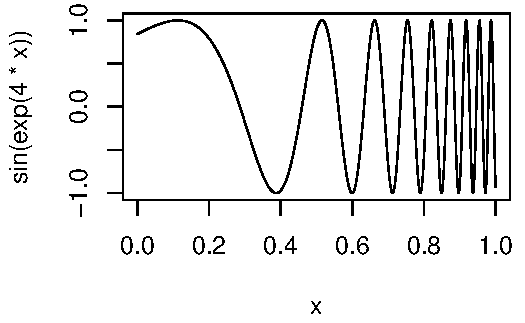
\includegraphics[width=0.7\linewidth]{Quotation_files/figure-latex/curve-demo-1} \end{center}

Here \texttt{x} is a pronoun: it doesn't represent a single concrete value, but is instead a placeholder that varies over the range of the plot. One way to implement \texttt{curve()} is to turn that expression into a function with a single argument, \texttt{x}, then call that function:

\begin{Shaded}
\begin{Highlighting}[]
\NormalTok{curve2 <-}\StringTok{ }\ControlFlowTok{function}\NormalTok{(expr, }\DataTypeTok{xlim =} \KeywordTok{c}\NormalTok{(}\DecValTok{0}\NormalTok{, }\DecValTok{1}\NormalTok{), }\DataTypeTok{n =} \DecValTok{100}\NormalTok{) \{}
\NormalTok{  expr <-}\StringTok{ }\KeywordTok{enexpr}\NormalTok{(expr)}
\NormalTok{  f <-}\StringTok{ }\KeywordTok{new_function}\NormalTok{(}\KeywordTok{exprs}\NormalTok{(}\DataTypeTok{x =}\NormalTok{ ), expr)}
  
\NormalTok{  x <-}\StringTok{ }\KeywordTok{seq}\NormalTok{(xlim[}\DecValTok{1}\NormalTok{], xlim[}\DecValTok{2}\NormalTok{], }\DataTypeTok{length =}\NormalTok{ n)}
\NormalTok{  y <-}\StringTok{ }\KeywordTok{f}\NormalTok{(x)}

  \KeywordTok{plot}\NormalTok{(x, y, }\DataTypeTok{type =} \StringTok{"l"}\NormalTok{, }\DataTypeTok{ylab =} \KeywordTok{expr_text}\NormalTok{(expr))}
\NormalTok{\}}
\KeywordTok{curve2}\NormalTok{(}\KeywordTok{sin}\NormalTok{(}\KeywordTok{exp}\NormalTok{(}\DecValTok{4} \OperatorTok{*}\StringTok{ }\NormalTok{x)), }\DataTypeTok{n =} \DecValTok{1000}\NormalTok{)}
\end{Highlighting}
\end{Shaded}

Functions like \texttt{curve()} that use an expression containing a pronoun are known as \textbf{anaphoric} functions\footnote{Anaphoric comes from the linguistics term ``anaphora'', an expression that is context dependent. Anaphoric functions are found in \href{http://www.arcfn.com/doc/anaphoric.html}{Arc} (a LISP like language), \href{http://www.perlmonks.org/index.pl?node_id=666047}{Perl}, and \href{http://amalloy.hubpages.com/hub/Unhygenic-anaphoric-Clojure-macros-for-fun-and-profit}{Clojure}.}.

\hypertarget{exercises-8}{%
\subsection{Exercises}\label{exercises-8}}

\begin{enumerate}
\def\labelenumi{\arabic{enumi}.}
\item
  In the linear-model example, we could replace the \texttt{expr()} in
  \texttt{reduce(summands,\ \textasciitilde{}\ expr(!!.x\ +\ !!.y))} with \texttt{call2()}:
  \texttt{reduce(summands,\ call2,\ "+")}. Compare and contrast the two
  approaches. Which do you think is easier to read?
\item
  Re-implement the Box-Cox transform defined below using unquoting and
  \texttt{new\_function()}:

\begin{Shaded}
\begin{Highlighting}[]
\NormalTok{bc <-}\StringTok{ }\ControlFlowTok{function}\NormalTok{(lambda) \{}
  \ControlFlowTok{if}\NormalTok{ (lambda }\OperatorTok{==}\StringTok{ }\DecValTok{0}\NormalTok{) \{}
    \ControlFlowTok{function}\NormalTok{(x) }\KeywordTok{log}\NormalTok{(x)}
\NormalTok{  \} }\ControlFlowTok{else}\NormalTok{ \{}
    \ControlFlowTok{function}\NormalTok{(x) (x }\OperatorTok{^}\StringTok{ }\NormalTok{lambda }\OperatorTok{-}\StringTok{ }\DecValTok{1}\NormalTok{) }\OperatorTok{/}\StringTok{ }\NormalTok{lambda}
\NormalTok{  \}}
\NormalTok{\}}
\end{Highlighting}
\end{Shaded}
\item
  Re-implement the simple \texttt{compose()} defined below using quasiquotation and
  \texttt{new\_function()}:

\begin{Shaded}
\begin{Highlighting}[]
\NormalTok{compose <-}\StringTok{ }\ControlFlowTok{function}\NormalTok{(f, g) \{}
  \ControlFlowTok{function}\NormalTok{(...) }\KeywordTok{f}\NormalTok{(}\KeywordTok{g}\NormalTok{(...))}
\NormalTok{\}}
\end{Highlighting}
\end{Shaded}
\end{enumerate}

\hypertarget{history}{%
\section{History}\label{history}}

The idea of quasiquotation is an old one. It was first developed by the philosopher Willard van Orman Quine\footnote{You might be familiar with the name Quine from ``quines'', computer programs that return a copy of their own source when run.} in the early 1940s. It's needed in philosophy\footnote{A fun connection between philosophy and R is in \url{https://johnmacfarlane.net/142/substitutional-quantifiers.pdf}; this article is written by philosophy professor John MacFarlane, the author of pandoc, which powers RMarkdown.} because it helps when precisely delineating the use and mention of words, i.e.~distinguishing between the object and the words we use to refer to that object.

Quasiquotation was first used in a programming language, LISP, in the mid-1970s (Bawden \protect\hyperlink{ref-bawden-1999}{1999}). LISP has one quoting function \texttt{\textasciigrave{}}, and uses \texttt{,} for unquoting. Most languages with a LISP heritage behave similarly. For example, racket (\texttt{\textasciigrave{}} and \texttt{@}), Clojure (\texttt{\textasciigrave{}} and \texttt{\textasciitilde{}}), and Julia (\texttt{:} and \texttt{@}) all have quasiquotation tools that differ only slightly from LISP. These languages have a single quoting function and you must call it explicitly.

In R, however, many functions quote one or more inputs. This introduces ambiguity (because you need to read the documentation to determine if an argument is quoted or not), but allows for concise and elegant data exploration code. In base R, only one function supports quasiquotation: \texttt{bquote()}, written in 2003 by Thomas Lumley. However, \texttt{bquote()} has some major limitations which prevented it from having a wide impact on R code (Section \ref{base-nonquote}).

My attempt to resolve these limitations lead to the lazyeval package (2014-2015). Unfortunately, my analysis of the problem was incomplete and while lazyeval solves some problems, it create others. It was not until I started working with Lionel Henry on the problem that all the pieces finally fell into place and we create the full tidy evaluation framework (2017). Despite the newness of tidy evaluation, I teach it here because it is a rich and powerful theory that, once mastered, makes many hard problems much easier.

\hypertarget{evaluation}{%
\chapter{Evaluation}\label{evaluation}}

\hypertarget{introduction-4}{%
\section{Introduction}\label{introduction-4}}

The user-facing inverse of quotation is unquotation: it gives the \emph{user} the ability to selectively evaluate parts of an otherwise quoted argument. The developer-facing complement of quotation is evaluation: this gives the \emph{developer} the ability to evaluate quoted expressions in custom environments to achieve specific goals.

This chapter begins with a discussion of evaluation in its purest form. You'll learn how \texttt{eval()} evaluates an expression in an environment, and then how it can be used to implement a number of important base R functions. Once you have the basics under your belt, you'll learn extensions to evaluation that are needed for robustness. There are two big new ideas:

\begin{itemize}
\item
  The quosure: a data structure that captures an expression along with its
  associated environment, as found in function arguments.
\item
  The data mask, which makes it easier to evaluate an expression in the
  context of a data frame. This introduces potential evaluation ambiguity
  which we'll then resolve with data pronouns.
\end{itemize}

Together, quasiquotation, quosures, and data masks form what we call \textbf{tidy evaluation}, or tidy eval for short. Tidy eval provides a principled approach to non-standard evaluation that makes it possible to use such functions both interactively and embedded with other functions. Tidy evaluation is the most important practical implication of all this theory so we'll spend a little time exploring the implications. The chapter finishes off with a discussion of the closest related approaches in base R, and how you can program around their drawbacks.

\hypertarget{outline-3}{%
\subsection*{Outline}\label{outline-3}}
\addcontentsline{toc}{subsection}{Outline}

\begin{itemize}
\item
  Section \ref{eval} discusses the basics of evaluation using \texttt{eval()},
  and shows how you can use it to implement key functions like \texttt{local()}
  and \texttt{source()}.
\item
  Section \ref{quosures} introduces a new data structure, the quosure, which
  combines an expression with an environment. You'll learn how to capture
  them from promises, and evaluate them using \texttt{rlang::eval\_tidy()}.
\item
  Section \ref{data-masks} extends evaluation with the ``data mask'', which
  makes it trivial to intermingle symbols bound in an environment with
  variables found in a data frame.
\item
  Section \ref{tidy-evaluation} shows how to use tidy evaluation in practice,
  focussing on the common pattern of quoting and unquoting, and how to
  handle ambiguity with pronouns.
\item
  Section \ref{base-evaluation} circles back to evaluation in base R,
  discusses some of the downsides, and shows how to use quasiquotation and
  evaluation to wrap functions that use NSE.
\end{itemize}

\hypertarget{prerequisites-3}{%
\subsection*{Prerequisites}\label{prerequisites-3}}
\addcontentsline{toc}{subsection}{Prerequisites}

You'll need to be familiar with the content of Chapter \ref{expressions} and Chapter \ref{quasiquotation}, as well as the environment data structure (Section \ref{env-basics}) and the caller environment (Section \ref{call-stack}).

We'll continue to use \href{https://rlang.r-lib.org}{rlang} and \href{https://purrr.tidyverse.org}{purrr}.

\begin{Shaded}
\begin{Highlighting}[]
\KeywordTok{library}\NormalTok{(rlang)}
\KeywordTok{library}\NormalTok{(purrr)}
\end{Highlighting}
\end{Shaded}

\hypertarget{eval}{%
\section{Evaluation basics}\label{eval}}

\index{evaluation!basics}
\indexc{eval\_bare()}

Here we'll explore the details of \texttt{eval()} which we briefly mentioned in the last chapter. It has two key arguments: \texttt{expr} and \texttt{envir}. The first argument, \texttt{expr}, is the object to evaluate, typically a symbol or expression\footnote{All other objects yield themselves when evaluated; i.e. \texttt{eval\_bare(x)} yields \texttt{x}, except when \texttt{x} is a symbol or expression.}. None of the evaluation functions quote their inputs, so you'll usually use them with \texttt{expr()} or similar:

\begin{Shaded}
\begin{Highlighting}[]
\NormalTok{x <-}\StringTok{ }\DecValTok{10}
\KeywordTok{eval}\NormalTok{(}\KeywordTok{expr}\NormalTok{(x))}
\CommentTok{#> [1] 10}

\NormalTok{y <-}\StringTok{ }\DecValTok{2}
\KeywordTok{eval}\NormalTok{(}\KeywordTok{expr}\NormalTok{(x }\OperatorTok{+}\StringTok{ }\NormalTok{y))}
\CommentTok{#> [1] 12}
\end{Highlighting}
\end{Shaded}

The second argument, \texttt{env}, gives the environment in which the expression should be evaluated, i.e.~where to look for the values of \texttt{x}, \texttt{y}, and \texttt{+}. By default, this is the current environment, i.e.~the calling environment of \texttt{eval()}, but you can override it if you want:

\begin{Shaded}
\begin{Highlighting}[]
\KeywordTok{eval}\NormalTok{(}\KeywordTok{expr}\NormalTok{(x }\OperatorTok{+}\StringTok{ }\NormalTok{y), }\KeywordTok{env}\NormalTok{(}\DataTypeTok{x =} \DecValTok{1000}\NormalTok{))}
\CommentTok{#> [1] 1002}
\end{Highlighting}
\end{Shaded}

The first argument is evaluated, not quoted, which can lead to confusing results once if you use a custom environment and forget to manually quote:

\begin{Shaded}
\begin{Highlighting}[]
\KeywordTok{eval}\NormalTok{(}\KeywordTok{print}\NormalTok{(x }\OperatorTok{+}\StringTok{ }\DecValTok{1}\NormalTok{), }\KeywordTok{env}\NormalTok{(}\DataTypeTok{x =} \DecValTok{1000}\NormalTok{))}
\CommentTok{#> [1] 11}
\CommentTok{#> [1] 11}

\KeywordTok{eval}\NormalTok{(}\KeywordTok{expr}\NormalTok{(}\KeywordTok{print}\NormalTok{(x }\OperatorTok{+}\StringTok{ }\DecValTok{1}\NormalTok{)), }\KeywordTok{env}\NormalTok{(}\DataTypeTok{x =} \DecValTok{1000}\NormalTok{))}
\CommentTok{#> [1] 1001}
\end{Highlighting}
\end{Shaded}

\textbf{Expression vectors}
\index{expression vectors}

\texttt{base::eval()} has special behaviour for expression \emph{vectors}, evaluating each component in turn. This makes for a very compact implementation of \texttt{source2()} because \texttt{base::parse()} also returns an expression object:

\begin{Shaded}
\begin{Highlighting}[]
\NormalTok{source3 <-}\StringTok{ }\ControlFlowTok{function}\NormalTok{(file, }\DataTypeTok{env =} \KeywordTok{parent.frame}\NormalTok{()) \{}
\NormalTok{  lines <-}\StringTok{ }\KeywordTok{parse}\NormalTok{(file)}
\NormalTok{  res <-}\StringTok{ }\KeywordTok{eval}\NormalTok{(lines, }\DataTypeTok{envir =}\NormalTok{ env)}
  \KeywordTok{invisible}\NormalTok{(res)}
\NormalTok{\}}
\end{Highlighting}
\end{Shaded}

While \texttt{source3()} is considerably more concise than \texttt{source2()}, this is the only advantage to expression vectors. Overall I don't believe this benefit outweighs the cost of introducing a new data structure, and hence this book avoids the use of expression vectors.

Now that you've seen the basics, let's explore some applications. We'll focus primarily on base R functions that you might have used before, reimplementing the underlying principles using rlang.

\hypertarget{application-local}{%
\subsection{\texorpdfstring{Application: \texttt{local()}}{Application: local()}}\label{application-local}}

\indexc{local()}

Sometimes you want to perform a chunk of calculation that creates some intermediate variables. The intermediate variables have no long-term use and could be quite large, so you'd rather not keep them around. One approach is to clean up after yourself using \texttt{rm()}; another is to wrap the code in a function and just call it once. A more elegant approach is to use \texttt{local()}:

\begin{Shaded}
\begin{Highlighting}[]
\CommentTok{# Clean up variables created earlier}
\KeywordTok{rm}\NormalTok{(x, y)}

\NormalTok{foo <-}\StringTok{ }\KeywordTok{local}\NormalTok{(\{}
\NormalTok{  x <-}\StringTok{ }\DecValTok{10}
\NormalTok{  y <-}\StringTok{ }\DecValTok{200}
\NormalTok{  x }\OperatorTok{+}\StringTok{ }\NormalTok{y}
\NormalTok{\})}

\NormalTok{foo}
\CommentTok{#> [1] 210}
\NormalTok{x}
\CommentTok{#> Error in eval(expr, envir, enclos): object 'x' not found}
\NormalTok{y}
\CommentTok{#> Error in eval(expr, envir, enclos): object 'y' not found}
\end{Highlighting}
\end{Shaded}

The essence of \texttt{local()} is quite simple and re-implemented below. We capture the input expression, and create a new environment in which to evaluate it. This is a new environment (so assignment doesn't affect the existing environment) with the caller environment as parent (so that \texttt{expr} can still access variables in that environment). This effectively emulates running \texttt{expr} as if it was inside a function (i.e.~it's lexically scoped, Section \ref{lexical-scoping}).

\begin{Shaded}
\begin{Highlighting}[]
\NormalTok{local2 <-}\StringTok{ }\ControlFlowTok{function}\NormalTok{(expr) \{}
\NormalTok{  env <-}\StringTok{ }\KeywordTok{env}\NormalTok{(}\KeywordTok{caller_env}\NormalTok{())}
  \KeywordTok{eval_bare}\NormalTok{(}\KeywordTok{enexpr}\NormalTok{(expr), env)}
\NormalTok{\}}

\NormalTok{foo <-}\StringTok{ }\KeywordTok{local2}\NormalTok{(\{}
\NormalTok{  x <-}\StringTok{ }\DecValTok{10}
\NormalTok{  y <-}\StringTok{ }\DecValTok{200}
\NormalTok{  x }\OperatorTok{+}\StringTok{ }\NormalTok{y}
\NormalTok{\})}

\NormalTok{foo}
\CommentTok{#> [1] 210}
\NormalTok{x}
\CommentTok{#> Error in eval(expr, envir, enclos): object 'x' not found}
\NormalTok{y}
\CommentTok{#> Error in eval(expr, envir, enclos): object 'y' not found}
\end{Highlighting}
\end{Shaded}

Understanding how \texttt{base::local()} works is harder, as it uses \texttt{eval()} and \texttt{substitute()} together in rather complicated ways. Figuring out exactly what's going on is good practice if you really want to understand the subtleties of \texttt{substitute()} and the base \texttt{eval()} functions, so is included in the exercises below.

\hypertarget{application-source}{%
\subsection{\texorpdfstring{Application: \texttt{source()}}{Application: source()}}\label{application-source}}

\indexc{source()}

We can create a simple version of \texttt{source()} by combining \texttt{eval()} with \texttt{parse\_expr()} from Section \ref{parsing}. We read in the file from disk, use \texttt{parse\_expr()} to parse the string into a list of expressions, and then use \texttt{eval\_bare()} to evaluate each element in turn. This version evaluates the code in the caller environment, and invisibly returns the result of the last expression in the file just like \texttt{base::source()}.

\begin{Shaded}
\begin{Highlighting}[]
\NormalTok{source2 <-}\StringTok{ }\ControlFlowTok{function}\NormalTok{(path, }\DataTypeTok{env =} \KeywordTok{caller_env}\NormalTok{()) \{}
\NormalTok{  file <-}\StringTok{ }\KeywordTok{paste}\NormalTok{(}\KeywordTok{readLines}\NormalTok{(path, }\DataTypeTok{warn =} \OtherTok{FALSE}\NormalTok{), }\DataTypeTok{collapse =} \StringTok{"}\CharTok{\textbackslash{}n}\StringTok{"}\NormalTok{)}
\NormalTok{  exprs <-}\StringTok{ }\KeywordTok{parse_exprs}\NormalTok{(file)}

\NormalTok{  res <-}\StringTok{ }\OtherTok{NULL}
  \ControlFlowTok{for}\NormalTok{ (i }\ControlFlowTok{in} \KeywordTok{seq_along}\NormalTok{(exprs)) \{}
\NormalTok{    res <-}\StringTok{ }\KeywordTok{eval}\NormalTok{(exprs[[i]], env)}
\NormalTok{  \}}

  \KeywordTok{invisible}\NormalTok{(res)}
\NormalTok{\}}
\end{Highlighting}
\end{Shaded}

The real \texttt{source()} is considerably more complicated because it can \texttt{echo} input and output, and has many other settings that control its behaviour.

\hypertarget{gotcha-function}{%
\subsection{\texorpdfstring{Gotcha: \texttt{function()}}{Gotcha: function()}}\label{gotcha-function}}

\index{evaluation!functions}
\indexc{srcref}

There's one small gotcha that you should be aware of if you're using \texttt{eval\_bare()} and \texttt{expr()} to generate functions:

\begin{Shaded}
\begin{Highlighting}[]
\NormalTok{x <-}\StringTok{ }\DecValTok{10}
\NormalTok{y <-}\StringTok{ }\DecValTok{20}
\NormalTok{f <-}\StringTok{ }\KeywordTok{eval}\NormalTok{(}\KeywordTok{expr}\NormalTok{(}\ControlFlowTok{function}\NormalTok{(x, y) }\OperatorTok{!!}\NormalTok{x }\OperatorTok{+}\StringTok{ }\OperatorTok{!!}\NormalTok{y))}
\NormalTok{f}
\CommentTok{#> function(x, y) !!x + !!y}
\end{Highlighting}
\end{Shaded}

This function doesn't look like it will work, but it does:

\begin{Shaded}
\begin{Highlighting}[]
\KeywordTok{f}\NormalTok{()}
\CommentTok{#> [1] 30}
\end{Highlighting}
\end{Shaded}

This is because, if available, functions print their \texttt{srcref} attribute (Section \ref{fun-components}), and because \texttt{srcref} is a base R feature it's unaware of quasiquotation.

To work around this problem, either use \texttt{new\_function()} (Section \ref{new-function}) or remove the \texttt{srcref} attribute:

\begin{Shaded}
\begin{Highlighting}[]
\KeywordTok{attr}\NormalTok{(f, }\StringTok{"srcref"}\NormalTok{) <-}\StringTok{ }\OtherTok{NULL}
\NormalTok{f}
\CommentTok{#> function (x, y) }
\CommentTok{#> 10 + 20}
\end{Highlighting}
\end{Shaded}

\hypertarget{exercises-9}{%
\subsection{Exercises}\label{exercises-9}}

\begin{enumerate}
\def\labelenumi{\arabic{enumi}.}
\item
  Carefully read the documentation for \texttt{source()}. What environment does it
  use by default? What if you supply \texttt{local\ =\ TRUE}? How do you provide
  a custom environment?
\item
  Predict the results of the following lines of code:

\begin{Shaded}
\begin{Highlighting}[]
\KeywordTok{eval}\NormalTok{(}\KeywordTok{expr}\NormalTok{(}\KeywordTok{eval}\NormalTok{(}\KeywordTok{expr}\NormalTok{(}\KeywordTok{eval}\NormalTok{(}\KeywordTok{expr}\NormalTok{(}\DecValTok{2} \OperatorTok{+}\StringTok{ }\DecValTok{2}\NormalTok{))))))}
\KeywordTok{eval}\NormalTok{(}\KeywordTok{eval}\NormalTok{(}\KeywordTok{expr}\NormalTok{(}\KeywordTok{eval}\NormalTok{(}\KeywordTok{expr}\NormalTok{(}\KeywordTok{eval}\NormalTok{(}\KeywordTok{expr}\NormalTok{(}\DecValTok{2} \OperatorTok{+}\StringTok{ }\DecValTok{2}\NormalTok{)))))))}
\KeywordTok{expr}\NormalTok{(}\KeywordTok{eval}\NormalTok{(}\KeywordTok{expr}\NormalTok{(}\KeywordTok{eval}\NormalTok{(}\KeywordTok{expr}\NormalTok{(}\KeywordTok{eval}\NormalTok{(}\KeywordTok{expr}\NormalTok{(}\DecValTok{2} \OperatorTok{+}\StringTok{ }\DecValTok{2}\NormalTok{)))))))}
\end{Highlighting}
\end{Shaded}
\item
  Fill in the function bodies below to re-implement \texttt{get()} using \texttt{sym()}
  and \texttt{eval()}, and\texttt{assign()} using \texttt{sym()}, \texttt{expr()}, and \texttt{eval()}. Don't
  worry about the multiple ways of choosing an environment that \texttt{get()} and
  \texttt{assign()} support; assume that the user supplies it explicitly

\begin{Shaded}
\begin{Highlighting}[]
\CommentTok{# name is a string}
\NormalTok{get2 <-}\StringTok{ }\ControlFlowTok{function}\NormalTok{(name, env) \{\}}
\NormalTok{assign2 <-}\StringTok{ }\ControlFlowTok{function}\NormalTok{(name, value, env) \{\}}
\end{Highlighting}
\end{Shaded}
\item
  Modify \texttt{source2()} so it returns the result of \emph{every} expression,
  not just the last one. Can you eliminate the for loop?
\item
  We can make \texttt{base::local()} slightly easier to understand by spreading
  out over multiple lines:

\begin{Shaded}
\begin{Highlighting}[]
\NormalTok{local3 <-}\StringTok{ }\ControlFlowTok{function}\NormalTok{(expr, }\DataTypeTok{envir =} \KeywordTok{new.env}\NormalTok{()) \{}
\NormalTok{  call <-}\StringTok{ }\KeywordTok{substitute}\NormalTok{(}\KeywordTok{eval}\NormalTok{(}\KeywordTok{quote}\NormalTok{(expr), envir))}
  \KeywordTok{eval}\NormalTok{(call, }\DataTypeTok{envir =} \KeywordTok{parent.frame}\NormalTok{())}
\NormalTok{\}}
\end{Highlighting}
\end{Shaded}

  Explain how \texttt{local()} works in words. (Hint: you might want to \texttt{print(call)}
  to help understand what \texttt{substitute()} is doing, and read the documentation
  to remind yourself what environment \texttt{new.env()} will inherit from.)
\end{enumerate}

\hypertarget{quosures}{%
\section{Quosures}\label{quosures}}

\index{quosures}

Almost every use of \texttt{eval()} involves both an expression and environment. This coupling is so important that we need a data structure that can hold both pieces. Base R does not have such a structure\footnote{Technically a formula combines an expression and environment, but formulas are tightly coupled to modelling so a new data structure makes sense.} so rlang fills the gap with the \textbf{quosure}, an object that contains an expression and an environment. The name is a portmanteau of quoting and closure, because a quosure both quotes the expression and encloses the environment. Quosures reify the internal promise object (Section \ref{promises}) into something that you can program with.

In this section, you'll learn how to create and manipulate quosures, and a little about how they are implemented.

\hypertarget{creating}{%
\subsection{Creating}\label{creating}}

\index{quosures!creating}

There are three ways to create quosures:

\begin{itemize}
\item
  Use \texttt{enquo()} and \texttt{enquos()} to capture user-supplied expressions.
  The vast majority of quosures should be created this way.

\begin{Shaded}
\begin{Highlighting}[]
\NormalTok{foo <-}\StringTok{ }\ControlFlowTok{function}\NormalTok{(x) }\KeywordTok{enquo}\NormalTok{(x)}
\KeywordTok{foo}\NormalTok{(a }\OperatorTok{+}\StringTok{ }\NormalTok{b)}
\CommentTok{#> <quosure>}
\CommentTok{#> expr: ^a + b}
\CommentTok{#> env:  global}
\end{Highlighting}
\end{Shaded}

  \indexc{enquo()}
\item
  \texttt{quo()} and \texttt{quos()} exist to match to \texttt{expr()} and \texttt{exprs()}, but
  they are included only for the sake of completeness and are needed very
  rarely. If you find yourself using them, think carefully if \texttt{expr()} and
  careful unquoting can eliminate the need to capture the environment.

\begin{Shaded}
\begin{Highlighting}[]
\KeywordTok{quo}\NormalTok{(x }\OperatorTok{+}\StringTok{ }\NormalTok{y }\OperatorTok{+}\StringTok{ }\NormalTok{z)}
\CommentTok{#> <quosure>}
\CommentTok{#> expr: ^x + y + z}
\CommentTok{#> env:  global}
\end{Highlighting}
\end{Shaded}

  \index{quosures!quo()@\texttt{quo()}}
\item
  \texttt{new\_quosure()} create a quosure from its components: an expression and
  an environment. This is rarely needed in practice, but is useful for
  learning, so is used a lot in this chapter.

\begin{Shaded}
\begin{Highlighting}[]
\KeywordTok{new_quosure}\NormalTok{(}\KeywordTok{expr}\NormalTok{(x }\OperatorTok{+}\StringTok{ }\NormalTok{y), }\KeywordTok{env}\NormalTok{(}\DataTypeTok{x =} \DecValTok{1}\NormalTok{, }\DataTypeTok{y =} \DecValTok{10}\NormalTok{))}
\CommentTok{#> <quosure>}
\CommentTok{#> expr: ^x + y}
\CommentTok{#> env:  0x60bcc58}
\end{Highlighting}
\end{Shaded}
\end{itemize}

\hypertarget{evaluating}{%
\subsection{Evaluating}\label{evaluating}}

\index{evaluation!tidy}
\index{quosures!evaluating}
\indexc{eval\_tidy()}

Quosures are paired with a new evaluation function \texttt{eval\_tidy()} that takes a single quosure instead of a expression-environment pair. It is straightforward to use:

\begin{Shaded}
\begin{Highlighting}[]
\NormalTok{q1 <-}\StringTok{ }\KeywordTok{new_quosure}\NormalTok{(}\KeywordTok{expr}\NormalTok{(x }\OperatorTok{+}\StringTok{ }\NormalTok{y), }\KeywordTok{env}\NormalTok{(}\DataTypeTok{x =} \DecValTok{1}\NormalTok{, }\DataTypeTok{y =} \DecValTok{10}\NormalTok{))}
\KeywordTok{eval_tidy}\NormalTok{(q1)}
\CommentTok{#> [1] 11}
\end{Highlighting}
\end{Shaded}

For this simple case, \texttt{eval\_tidy(q1)} is basically a shortcut for \texttt{eval\_bare(get\_expr(q1),\ get\_env(q2))}. However, it has two important features that you'll learn about later in the chapter: it supports nested quosures (Section \ref{nested-quosures}) and pronouns (Section \ref{pronouns}).

\hypertarget{quosure-dots}{%
\subsection{Dots}\label{quosure-dots}}

\indexc{...}

Quosures are typically just a convenience: they make code cleaner because you only have one object to pass around, instead of two. They are, however, essential when it comes to working with \texttt{...} because it's possible for each argument passed to \ldots{} to be associated with a different environment. In the following example note that both quosures have the same expression, \texttt{x}, but a different environment:

\begin{Shaded}
\begin{Highlighting}[]
\NormalTok{f <-}\StringTok{ }\ControlFlowTok{function}\NormalTok{(...) \{}
\NormalTok{  x <-}\StringTok{ }\DecValTok{1}
  \KeywordTok{g}\NormalTok{(..., }\DataTypeTok{f =}\NormalTok{ x)}
\NormalTok{\}}
\NormalTok{g <-}\StringTok{ }\ControlFlowTok{function}\NormalTok{(...) \{}
  \KeywordTok{enquos}\NormalTok{(...)}
\NormalTok{\}}

\NormalTok{x <-}\StringTok{ }\DecValTok{0}
\NormalTok{qs <-}\StringTok{ }\KeywordTok{f}\NormalTok{(}\DataTypeTok{global =}\NormalTok{ x)}
\NormalTok{qs}
\CommentTok{#> <list_of<quosure>>}
\CommentTok{#> }
\CommentTok{#> $global}
\CommentTok{#> <quosure>}
\CommentTok{#> expr: ^x}
\CommentTok{#> env:  global}
\CommentTok{#> }
\CommentTok{#> $f}
\CommentTok{#> <quosure>}
\CommentTok{#> expr: ^x}
\CommentTok{#> env:  0x68d54e8}
\end{Highlighting}
\end{Shaded}

That means that when you evaluate them, you get the correct results:

\begin{Shaded}
\begin{Highlighting}[]
\KeywordTok{map_dbl}\NormalTok{(qs, eval_tidy)}
\CommentTok{#> global      f }
\CommentTok{#>      0      1}
\end{Highlighting}
\end{Shaded}

Correctly evaluating the elements of \texttt{...} was one of the original motivations for the development of quosures.

\hypertarget{quosure-impl}{%
\subsection{Under the hood}\label{quosure-impl}}

\index{quosures!internals}
\index{formulas}

Quosures were inspired by R's formulas, because formulas capture an expression and an environment:

\begin{Shaded}
\begin{Highlighting}[]
\NormalTok{f <-}\StringTok{ }\ErrorTok{~}\KeywordTok{runif}\NormalTok{(}\DecValTok{3}\NormalTok{)}
\KeywordTok{str}\NormalTok{(f)}
\CommentTok{#> Class 'formula'  language ~runif(3)}
\CommentTok{#>   ..- attr(*, ".Environment")=<environment: R_GlobalEnv>}
\end{Highlighting}
\end{Shaded}

An early version of tidy evaluation used formulas instead of quosures, as an attractive feature of \texttt{\textasciitilde{}} is that it provides quoting with a single keystroke. Unfortunately, however, there is no clean way to make \texttt{\textasciitilde{}} a quasiquoting function.

Quosures are a subclass of formulas:

\begin{Shaded}
\begin{Highlighting}[]
\NormalTok{q4 <-}\StringTok{ }\KeywordTok{new_quosure}\NormalTok{(}\KeywordTok{expr}\NormalTok{(x }\OperatorTok{+}\StringTok{ }\NormalTok{y }\OperatorTok{+}\StringTok{ }\NormalTok{z))}
\KeywordTok{class}\NormalTok{(q4)}
\CommentTok{#> [1] "quosure" "formula"}
\end{Highlighting}
\end{Shaded}

Which means that under the hood, quosures, like formulas, are a call object:

\begin{Shaded}
\begin{Highlighting}[]
\KeywordTok{is_call}\NormalTok{(q4)}
\CommentTok{#> [1] TRUE}

\NormalTok{q4[[}\DecValTok{1}\NormalTok{]]}
\CommentTok{#> `~`}
\NormalTok{q4[[}\DecValTok{2}\NormalTok{]]}
\CommentTok{#> x + y + z}
\end{Highlighting}
\end{Shaded}

With an attribute that stores the environment:

\begin{Shaded}
\begin{Highlighting}[]
\KeywordTok{attr}\NormalTok{(q4, }\StringTok{".Environment"}\NormalTok{)}
\CommentTok{#> <environment: R_GlobalEnv>}
\end{Highlighting}
\end{Shaded}

If you need to extract the expression or environment, don't rely on these implementation details. Instead use \texttt{get\_expr()} and \texttt{get\_env()}:

\begin{Shaded}
\begin{Highlighting}[]
\KeywordTok{get_expr}\NormalTok{(q4)}
\CommentTok{#> x + y + z}
\KeywordTok{get_env}\NormalTok{(q4)}
\CommentTok{#> <environment: R_GlobalEnv>}
\end{Highlighting}
\end{Shaded}

\hypertarget{nested-quosures}{%
\subsection{Nested quosures}\label{nested-quosures}}

\index{quosures!nested}

It's possible to use quasiquotation to embed a quosure in an expression. This is an advanced tool, and most of the time you don't need to think about it because it just works, but I talk about it here so you can spot nested quosures in the wild and not be confused. Take this example, which inlines two quosures into an expression:

\begin{Shaded}
\begin{Highlighting}[]
\NormalTok{q2 <-}\StringTok{ }\KeywordTok{new_quosure}\NormalTok{(}\KeywordTok{expr}\NormalTok{(x), }\KeywordTok{env}\NormalTok{(}\DataTypeTok{x =} \DecValTok{1}\NormalTok{))}
\NormalTok{q3 <-}\StringTok{ }\KeywordTok{new_quosure}\NormalTok{(}\KeywordTok{expr}\NormalTok{(x), }\KeywordTok{env}\NormalTok{(}\DataTypeTok{x =} \DecValTok{10}\NormalTok{))}

\NormalTok{x <-}\StringTok{ }\KeywordTok{expr}\NormalTok{(}\OperatorTok{!!}\NormalTok{q2 }\OperatorTok{+}\StringTok{ }\OperatorTok{!!}\NormalTok{q3)}
\end{Highlighting}
\end{Shaded}

It evaluates correctly with \texttt{eval\_tidy()}:

\begin{Shaded}
\begin{Highlighting}[]
\KeywordTok{eval_tidy}\NormalTok{(x)}
\CommentTok{#> [1] 11}
\end{Highlighting}
\end{Shaded}

However, if you print it, you only see the \texttt{x}s, with their formula heritage leaking through:

\begin{Shaded}
\begin{Highlighting}[]
\NormalTok{x}
\CommentTok{#> (~x) + ~x}
\end{Highlighting}
\end{Shaded}

You can get a better display with \texttt{rlang::expr\_print()} (Section \ref{non-standard-ast}):

\begin{Shaded}
\begin{Highlighting}[]
\KeywordTok{expr_print}\NormalTok{(x)}
\CommentTok{#> (^x) + (^x)}
\end{Highlighting}
\end{Shaded}

When you use \texttt{expr\_print()} in the console, quosures are coloured according to their environment, making it easier to spot when symbols are bound to different variables.

\hypertarget{exercises-10}{%
\subsection{Exercises}\label{exercises-10}}

\begin{enumerate}
\def\labelenumi{\arabic{enumi}.}
\item
  Predict what evaluating each of the following quosures will return if
  evaluated.

\begin{Shaded}
\begin{Highlighting}[]
\NormalTok{q1 <-}\StringTok{ }\KeywordTok{new_quosure}\NormalTok{(}\KeywordTok{expr}\NormalTok{(x), }\KeywordTok{env}\NormalTok{(}\DataTypeTok{x =} \DecValTok{1}\NormalTok{))}
\NormalTok{q1}
\CommentTok{#> <quosure>}
\CommentTok{#> expr: ^x}
\CommentTok{#> env:  0x5fa5830}

\NormalTok{q2 <-}\StringTok{ }\KeywordTok{new_quosure}\NormalTok{(}\KeywordTok{expr}\NormalTok{(x }\OperatorTok{+}\StringTok{ }\OperatorTok{!!}\NormalTok{q1), }\KeywordTok{env}\NormalTok{(}\DataTypeTok{x =} \DecValTok{10}\NormalTok{))}
\NormalTok{q2}
\CommentTok{#> <quosure>}
\CommentTok{#> expr: ^x + (^x)}
\CommentTok{#> env:  0x6143180}

\NormalTok{q3 <-}\StringTok{ }\KeywordTok{new_quosure}\NormalTok{(}\KeywordTok{expr}\NormalTok{(x }\OperatorTok{+}\StringTok{ }\OperatorTok{!!}\NormalTok{q2), }\KeywordTok{env}\NormalTok{(}\DataTypeTok{x =} \DecValTok{100}\NormalTok{))}
\NormalTok{q3}
\CommentTok{#> <quosure>}
\CommentTok{#> expr: ^x + (^x + (^x))}
\CommentTok{#> env:  0x63cb480}
\end{Highlighting}
\end{Shaded}
\item
  Write an \texttt{enenv()} function that captures the environment associated
  with an argument. (Hint: this should only require two function calls.)
\end{enumerate}

\hypertarget{data-masks}{%
\section{Data masks}\label{data-masks}}

\index{data masks}

In this section, you'll learn about the \textbf{data mask}, a data frame where the evaluated code will look first for variable definitions. The data mask is the key idea that powers base functions like \texttt{with()}, \texttt{subset()} and \texttt{transform()}, and is used throughout the tidyverse in packages like dplyr and ggplot2.

\hypertarget{basics}{%
\subsection{Basics}\label{basics}}

\indexc{eval\_tidy()}

The data mask allows you to mingle variables from an environment and and data frame in a single expression. You supply the data mask as the second argument to \texttt{eval\_tidy()}:

\begin{Shaded}
\begin{Highlighting}[]
\NormalTok{q1 <-}\StringTok{ }\KeywordTok{new_quosure}\NormalTok{(}\KeywordTok{expr}\NormalTok{(x }\OperatorTok{*}\StringTok{ }\NormalTok{y), }\KeywordTok{env}\NormalTok{(}\DataTypeTok{x =} \DecValTok{100}\NormalTok{))}
\NormalTok{df <-}\StringTok{ }\KeywordTok{data.frame}\NormalTok{(}\DataTypeTok{y =} \DecValTok{1}\OperatorTok{:}\DecValTok{10}\NormalTok{)}

\KeywordTok{eval_tidy}\NormalTok{(q1, df)}
\CommentTok{#>  [1]  100  200  300  400  500  600  700  800  900 1000}
\end{Highlighting}
\end{Shaded}

This code is a little hard to follow because there's so much syntax as we're creating every object from from scratch. It's easier to see what's going on if we make a little wrapper. I call this \texttt{with2()} because it's equivalent to \texttt{base::with()}.
\indexc{with()}

\begin{Shaded}
\begin{Highlighting}[]
\NormalTok{with2 <-}\StringTok{ }\ControlFlowTok{function}\NormalTok{(data, expr) \{}
\NormalTok{  expr <-}\StringTok{ }\KeywordTok{enquo}\NormalTok{(expr)}
  \KeywordTok{eval_tidy}\NormalTok{(expr, data)}
\NormalTok{\}}
\end{Highlighting}
\end{Shaded}

We can now rewrite the code above as below:

\begin{Shaded}
\begin{Highlighting}[]
\NormalTok{x <-}\StringTok{ }\DecValTok{100}
\KeywordTok{with2}\NormalTok{(df, x }\OperatorTok{*}\StringTok{ }\NormalTok{y)}
\CommentTok{#>  [1]  100  200  300  400  500  600  700  800  900 1000}
\end{Highlighting}
\end{Shaded}

\texttt{base::eval()} has similar functionality, although it doesn't call it a data mask. Instead you can supply a data frame to the second argument and an environment to the third. That gives the following implementation of \texttt{with()}:

\begin{Shaded}
\begin{Highlighting}[]
\NormalTok{with3 <-}\StringTok{ }\ControlFlowTok{function}\NormalTok{(data, expr) \{}
\NormalTok{  expr <-}\StringTok{ }\KeywordTok{substitute}\NormalTok{(expr)}
  \KeywordTok{eval}\NormalTok{(expr, data, }\KeywordTok{caller_env}\NormalTok{())}
\NormalTok{\}}
\end{Highlighting}
\end{Shaded}

\hypertarget{pronouns}{%
\subsection{Pronouns}\label{pronouns}}

\index{pronouns}
\index{.Data@\texttt{.data}}
\index{.Env@\texttt{.env}}

Using a data mask introduces ambiguity. For example, in the following code you can't know whether \texttt{x} will come from the data mask or the environment, unless you know what variables are found in \texttt{df}.

\begin{Shaded}
\begin{Highlighting}[]
\KeywordTok{with2}\NormalTok{(df, x)}
\end{Highlighting}
\end{Shaded}

That makes code harder to reason about (because you need to know more context), which can introduce bugs. To resolve that issue, the data mask provides two pronouns: \texttt{.data} and \texttt{.env}.

\begin{itemize}
\tightlist
\item
  \texttt{.data\$x} always refers to \texttt{x} in the data mask.
\item
  \texttt{.env\$x} always refers to \texttt{x} in the environment.
\end{itemize}

\begin{Shaded}
\begin{Highlighting}[]
\NormalTok{x <-}\StringTok{ }\DecValTok{1}
\NormalTok{df <-}\StringTok{ }\KeywordTok{data.frame}\NormalTok{(}\DataTypeTok{x =} \DecValTok{2}\NormalTok{)}

\KeywordTok{with2}\NormalTok{(df, .data}\OperatorTok{$}\NormalTok{x)}
\CommentTok{#> [1] 2}
\KeywordTok{with2}\NormalTok{(df, .env}\OperatorTok{$}\NormalTok{x)}
\CommentTok{#> [1] 1}
\end{Highlighting}
\end{Shaded}

You can also subset \texttt{.data} and \texttt{.env} using \texttt{{[}{[}}, e.g. \texttt{.data{[}{[}"x"{]}{]}}. Otherwise the pronouns are special objects and you shouldn't expect them to behave like data frames or environments. In particular, they throw error if the object isn't found:

\begin{Shaded}
\begin{Highlighting}[]
\KeywordTok{with2}\NormalTok{(df, .data}\OperatorTok{$}\NormalTok{y)}
\CommentTok{#> Error: Column `y` not found in `.data`}
\end{Highlighting}
\end{Shaded}

\hypertarget{subset}{%
\subsection{\texorpdfstring{Application: \texttt{subset()}}{Application: subset()}}\label{subset}}

\indexc{subset()}
\indexc{filter()}

We'll explore tidy evaluation in the context of \texttt{base::subset()}, because it's a simple yet powerful function that makes a common data manipulation challenge easier. If you haven't used it before, \texttt{subset()}, like \texttt{dplyr::filter()}, provides a convenient way of selecting rows of a data frame. You give it some data, along with an expression that is evaluated in the context of that data. This considerably reduces the number of times you need to type the name of the data frame:

\begin{Shaded}
\begin{Highlighting}[]
\NormalTok{sample_df <-}\StringTok{ }\KeywordTok{data.frame}\NormalTok{(}\DataTypeTok{a =} \DecValTok{1}\OperatorTok{:}\DecValTok{5}\NormalTok{, }\DataTypeTok{b =} \DecValTok{5}\OperatorTok{:}\DecValTok{1}\NormalTok{, }\DataTypeTok{c =} \KeywordTok{c}\NormalTok{(}\DecValTok{5}\NormalTok{, }\DecValTok{3}\NormalTok{, }\DecValTok{1}\NormalTok{, }\DecValTok{4}\NormalTok{, }\DecValTok{1}\NormalTok{))}

\CommentTok{# Shorthand for sample_df[sample_df$a >= 4, ]}
\KeywordTok{subset}\NormalTok{(sample_df, a }\OperatorTok{>=}\StringTok{ }\DecValTok{4}\NormalTok{)}
\CommentTok{#>   a b c}
\CommentTok{#> 4 4 2 4}
\CommentTok{#> 5 5 1 1}

\CommentTok{# Shorthand for sample_df[sample_df$b == sample_df$c, ]}
\KeywordTok{subset}\NormalTok{(sample_df, b }\OperatorTok{==}\StringTok{ }\NormalTok{c)}
\CommentTok{#>   a b c}
\CommentTok{#> 1 1 5 5}
\CommentTok{#> 5 5 1 1}
\end{Highlighting}
\end{Shaded}

The core of our version of \texttt{subset()}, \texttt{subset2()}, is quite simple. It takes two arguments: a data frame, \texttt{data}, and an expression, \texttt{rows}. We evaluate \texttt{rows} using \texttt{df} as a data mask, then use the results to subset the data frame with \texttt{{[}}. I've included a very simple check to ensure the result is a logical vector; real code would do more to create an informative error.

\begin{Shaded}
\begin{Highlighting}[]
\NormalTok{subset2 <-}\StringTok{ }\ControlFlowTok{function}\NormalTok{(data, rows) \{}
\NormalTok{  rows <-}\StringTok{ }\KeywordTok{enquo}\NormalTok{(rows)}
\NormalTok{  rows_val <-}\StringTok{ }\KeywordTok{eval_tidy}\NormalTok{(rows, data)}
  \KeywordTok{stopifnot}\NormalTok{(}\KeywordTok{is.logical}\NormalTok{(rows_val))}

\NormalTok{  data[rows_val, , drop =}\StringTok{ }\OtherTok{FALSE}\NormalTok{]}
\NormalTok{\}}

\KeywordTok{subset2}\NormalTok{(sample_df, b }\OperatorTok{==}\StringTok{ }\NormalTok{c)}
\CommentTok{#>   a b c}
\CommentTok{#> 1 1 5 5}
\CommentTok{#> 5 5 1 1}
\end{Highlighting}
\end{Shaded}

\hypertarget{application-transform}{%
\subsection{Application: transform}\label{application-transform}}

\indexc{transform()}

A more complicated situation is \texttt{base::transform()} which allows you to add new variables to a data frame, evaluating their expressions in the context of the existing variables:

\begin{Shaded}
\begin{Highlighting}[]
\NormalTok{df <-}\StringTok{ }\KeywordTok{data.frame}\NormalTok{(}\DataTypeTok{x =} \KeywordTok{c}\NormalTok{(}\DecValTok{2}\NormalTok{, }\DecValTok{3}\NormalTok{, }\DecValTok{1}\NormalTok{), }\DataTypeTok{y =} \KeywordTok{runif}\NormalTok{(}\DecValTok{3}\NormalTok{))}
\KeywordTok{transform}\NormalTok{(df, }\DataTypeTok{x =} \OperatorTok{-}\NormalTok{x, }\DataTypeTok{y2 =} \DecValTok{2} \OperatorTok{*}\StringTok{ }\NormalTok{y)}
\CommentTok{#>    x      y    y2}
\CommentTok{#> 1 -2 0.0808 0.162}
\CommentTok{#> 2 -3 0.8343 1.669}
\CommentTok{#> 3 -1 0.6008 1.202}
\end{Highlighting}
\end{Shaded}

Again, our own \texttt{transform2()} requires little code. We capture the unevalated \texttt{...} with \texttt{enquos(...)}, and then evaluate each expression using a for loop. Real code would do more error checking to ensure that each input is named and evaluates to a vector the same length as \texttt{data}.

\begin{Shaded}
\begin{Highlighting}[]
\NormalTok{transform2 <-}\StringTok{ }\ControlFlowTok{function}\NormalTok{(.data, ...) \{}
\NormalTok{  dots <-}\StringTok{ }\KeywordTok{enquos}\NormalTok{(...)}

  \ControlFlowTok{for}\NormalTok{ (i }\ControlFlowTok{in} \KeywordTok{seq_along}\NormalTok{(dots)) \{}
\NormalTok{    name <-}\StringTok{ }\KeywordTok{names}\NormalTok{(dots)[[i]]}
\NormalTok{    dot <-}\StringTok{ }\NormalTok{dots[[i]]}

\NormalTok{    .data[[name]] <-}\StringTok{ }\KeywordTok{eval_tidy}\NormalTok{(dot, .data)}
\NormalTok{  \}}

\NormalTok{  .data}
\NormalTok{\}}

\KeywordTok{transform2}\NormalTok{(df, }\DataTypeTok{x2 =}\NormalTok{ x }\OperatorTok{*}\StringTok{ }\DecValTok{2}\NormalTok{, }\DataTypeTok{y =} \OperatorTok{-}\NormalTok{y)}
\CommentTok{#>   x       y x2}
\CommentTok{#> 1 2 -0.0808  4}
\CommentTok{#> 2 3 -0.8343  6}
\CommentTok{#> 3 1 -0.6008  2}
\end{Highlighting}
\end{Shaded}

NB: I named the first argument \texttt{.data} to avoid problems if the user tried to create a variable called \texttt{data}. They will still have problems if they attempt to create a variable called \texttt{.data}, but this is much less likely. This is the same reasoning that leads to the \texttt{.x} and \texttt{.f} arguments to \texttt{map()} (Section \ref{argument-names}).

\hypertarget{select}{%
\subsection{\texorpdfstring{Application: \texttt{select()}}{Application: select()}}\label{select}}

\indexc{select()}

A data mask will typically be a data frame, but it's sometimes useful to provide a list filled with more exotic contents. This is basically how the \texttt{select} argument in \texttt{base::subset()} works. It allows you to refer to variables as if they were numbers:

\begin{Shaded}
\begin{Highlighting}[]
\NormalTok{df <-}\StringTok{ }\KeywordTok{data.frame}\NormalTok{(}\DataTypeTok{a =} \DecValTok{1}\NormalTok{, }\DataTypeTok{b =} \DecValTok{2}\NormalTok{, }\DataTypeTok{c =} \DecValTok{3}\NormalTok{, }\DataTypeTok{d =} \DecValTok{4}\NormalTok{, }\DataTypeTok{e =} \DecValTok{5}\NormalTok{)}
\KeywordTok{subset}\NormalTok{(df, }\DataTypeTok{select =}\NormalTok{ b}\OperatorTok{:}\NormalTok{d)}
\CommentTok{#>   b c d}
\CommentTok{#> 1 2 3 4}
\end{Highlighting}
\end{Shaded}

The key idea is to create a named list where each component gives the position of the corresponding variable:

\begin{Shaded}
\begin{Highlighting}[]
\NormalTok{vars <-}\StringTok{ }\KeywordTok{as.list}\NormalTok{(}\KeywordTok{set_names}\NormalTok{(}\KeywordTok{seq_along}\NormalTok{(df), }\KeywordTok{names}\NormalTok{(df)))}
\KeywordTok{str}\NormalTok{(vars)}
\CommentTok{#> List of 5}
\CommentTok{#>  $ a: int 1}
\CommentTok{#>  $ b: int 2}
\CommentTok{#>  $ c: int 3}
\CommentTok{#>  $ d: int 4}
\CommentTok{#>  $ e: int 5}
\end{Highlighting}
\end{Shaded}

Then implementation is again only a few lines of code:

\begin{Shaded}
\begin{Highlighting}[]
\NormalTok{select2 <-}\StringTok{ }\ControlFlowTok{function}\NormalTok{(data, ...) \{}
\NormalTok{  dots <-}\StringTok{ }\KeywordTok{enquos}\NormalTok{(...)}

\NormalTok{  vars <-}\StringTok{ }\KeywordTok{as.list}\NormalTok{(}\KeywordTok{set_names}\NormalTok{(}\KeywordTok{seq_along}\NormalTok{(data), }\KeywordTok{names}\NormalTok{(data)))}
\NormalTok{  cols <-}\StringTok{ }\KeywordTok{unlist}\NormalTok{(}\KeywordTok{map}\NormalTok{(dots, eval_tidy, vars))}

\NormalTok{  df[, cols, drop =}\StringTok{ }\OtherTok{FALSE}\NormalTok{]}
\NormalTok{\}}
\KeywordTok{select2}\NormalTok{(df, b}\OperatorTok{:}\NormalTok{d)}
\CommentTok{#>   b c d}
\CommentTok{#> 1 2 3 4}
\end{Highlighting}
\end{Shaded}

\texttt{dplyr::select()} takes this idea and runs with it, providing a number of helpers that allow you to select variables based on their names (e.g. \texttt{starts\_with("x")} or \texttt{ends\_with("\_a"})).

\hypertarget{exercises-11}{%
\subsection{Exercises}\label{exercises-11}}

\begin{enumerate}
\def\labelenumi{\arabic{enumi}.}
\item
  Why did I use a for loop in \texttt{transform2()} instead of \texttt{map()}?
  Consider \texttt{transform2(df,\ x\ =\ x\ *\ 2,\ x\ =\ x\ *\ 2)}.
\item
  Here's an alternative implementation of \texttt{subset2()}:

\begin{Shaded}
\begin{Highlighting}[]
\NormalTok{subset3 <-}\StringTok{ }\ControlFlowTok{function}\NormalTok{(data, rows) \{}
\NormalTok{  rows <-}\StringTok{ }\KeywordTok{enquo}\NormalTok{(rows)}
  \KeywordTok{eval_tidy}\NormalTok{(}\KeywordTok{expr}\NormalTok{(data[}\OperatorTok{!!}\NormalTok{rows, , }\DataTypeTok{drop =} \OtherTok{FALSE}\NormalTok{]), }\DataTypeTok{data =}\NormalTok{ data)}
\NormalTok{\}}

\NormalTok{df <-}\StringTok{ }\KeywordTok{data.frame}\NormalTok{(}\DataTypeTok{x =} \DecValTok{1}\OperatorTok{:}\DecValTok{3}\NormalTok{)}
\KeywordTok{subset3}\NormalTok{(df, x }\OperatorTok{==}\StringTok{ }\DecValTok{1}\NormalTok{)}
\end{Highlighting}
\end{Shaded}

  Compare and contrast \texttt{subset3()} to \texttt{subset2()}. What are its advantages
  and disadvantages?
\item
  The following function implements the basics of \texttt{dplyr::arrange()}.
  Annotate each line with a comment explaining what it does. Can you
  explain why \texttt{!!.na.last} is strictly correct, but omitting the \texttt{!!}
  is unlikely to cause problems?

\begin{Shaded}
\begin{Highlighting}[]
\NormalTok{arrange2 <-}\StringTok{ }\ControlFlowTok{function}\NormalTok{(.df, ..., }\DataTypeTok{.na.last =} \OtherTok{TRUE}\NormalTok{) \{}
\NormalTok{  args <-}\StringTok{ }\KeywordTok{enquos}\NormalTok{(...)}

\NormalTok{  order_call <-}\StringTok{ }\KeywordTok{expr}\NormalTok{(}\KeywordTok{order}\NormalTok{(}\OperatorTok{!!!}\NormalTok{args, }\DataTypeTok{na.last =} \OperatorTok{!!}\NormalTok{.na.last))}

\NormalTok{  ord <-}\StringTok{ }\KeywordTok{eval_tidy}\NormalTok{(order_call, .df)}
  \KeywordTok{stopifnot}\NormalTok{(}\KeywordTok{length}\NormalTok{(ord) }\OperatorTok{==}\StringTok{ }\KeywordTok{nrow}\NormalTok{(.df))}

\NormalTok{  .df[ord, , drop =}\StringTok{ }\OtherTok{FALSE}\NormalTok{]}
\NormalTok{\}}
\end{Highlighting}
\end{Shaded}
\end{enumerate}

\hypertarget{tidy-evaluation}{%
\section{Using tidy evaluation}\label{tidy-evaluation}}

While it's important to understand how \texttt{eval\_tidy()} works, most of the time you won't call it directly. Instead, you'll usually use it indirectly by calling a function that uses \texttt{eval\_tidy()}. This section will give a few practical examples of wrapping functions that use tidy evaluation.

\hypertarget{quoting-and-unquoting}{%
\subsection{Quoting and unquoting}\label{quoting-and-unquoting}}

\index{quoting!in practice}
\index{unquoting!in practice}
\index{bootstrapping}

Imagine we have written a function that resamples a dataset:

\begin{Shaded}
\begin{Highlighting}[]
\NormalTok{resample <-}\StringTok{ }\ControlFlowTok{function}\NormalTok{(df, n) \{}
\NormalTok{  idx <-}\StringTok{ }\KeywordTok{sample}\NormalTok{(}\KeywordTok{nrow}\NormalTok{(df), n, }\DataTypeTok{replace =} \OtherTok{TRUE}\NormalTok{)}
\NormalTok{  df[idx, , drop =}\StringTok{ }\OtherTok{FALSE}\NormalTok{]}
\NormalTok{\}}
\end{Highlighting}
\end{Shaded}

We want to create a new function that allows us to resample and subset in a single step. Our naive approach doesn't work:

\begin{Shaded}
\begin{Highlighting}[]
\NormalTok{subsample <-}\StringTok{ }\ControlFlowTok{function}\NormalTok{(df, cond, }\DataTypeTok{n =} \KeywordTok{nrow}\NormalTok{(df)) \{}
\NormalTok{  df <-}\StringTok{ }\KeywordTok{subset2}\NormalTok{(df, cond)}
  \KeywordTok{resample}\NormalTok{(df, n)}
\NormalTok{\}}

\NormalTok{df <-}\StringTok{ }\KeywordTok{data.frame}\NormalTok{(}\DataTypeTok{x =} \KeywordTok{c}\NormalTok{(}\DecValTok{1}\NormalTok{, }\DecValTok{1}\NormalTok{, }\DecValTok{1}\NormalTok{, }\DecValTok{2}\NormalTok{, }\DecValTok{2}\NormalTok{), }\DataTypeTok{y =} \DecValTok{1}\OperatorTok{:}\DecValTok{5}\NormalTok{)}
\KeywordTok{subsample}\NormalTok{(df, x }\OperatorTok{==}\StringTok{ }\DecValTok{1}\NormalTok{)}
\CommentTok{#> Error in eval_tidy(rows, data): object 'x' not found}
\end{Highlighting}
\end{Shaded}

\texttt{subsample()} doesn't quote any arguments so \texttt{cond} is evaluated normally (not in a data mask), and we get an error when it tries to find a binding for \texttt{x}. To fix this problem we need to quote \texttt{cond}, and then unquote it when we pass it on ot \texttt{subset2()}:

\begin{Shaded}
\begin{Highlighting}[]
\NormalTok{subsample <-}\StringTok{ }\ControlFlowTok{function}\NormalTok{(df, cond, }\DataTypeTok{n =} \KeywordTok{nrow}\NormalTok{(df)) \{}
\NormalTok{  cond <-}\StringTok{ }\KeywordTok{enquo}\NormalTok{(cond)}

\NormalTok{  df <-}\StringTok{ }\KeywordTok{subset2}\NormalTok{(df, }\OperatorTok{!!}\NormalTok{cond)}
  \KeywordTok{resample}\NormalTok{(df, n)}
\NormalTok{\}}

\KeywordTok{subsample}\NormalTok{(df, x }\OperatorTok{==}\StringTok{ }\DecValTok{1}\NormalTok{)}
\CommentTok{#>     x y}
\CommentTok{#> 1   1 1}
\CommentTok{#> 1.1 1 1}
\CommentTok{#> 2   1 2}
\end{Highlighting}
\end{Shaded}

This is a very common pattern; whenever you call a quoting function with arguments from the user, you need to quote them yourself and then unquote.

\hypertarget{handling-ambiguity}{%
\subsection{Handling ambiguity}\label{handling-ambiguity}}

\index{pronouns}

In the case above, we needed to think about tidy evaluation because of quasiquotation. We also need to think about tidy evaluation even when the wrapper doesn't need to quote any arguments. Take this wrapper around \texttt{subset2()}:

\begin{Shaded}
\begin{Highlighting}[]
\NormalTok{threshold_x <-}\StringTok{ }\ControlFlowTok{function}\NormalTok{(df, val) \{}
  \KeywordTok{subset2}\NormalTok{(df, x }\OperatorTok{>=}\StringTok{ }\NormalTok{val)}
\NormalTok{\}}
\end{Highlighting}
\end{Shaded}

This function can silently return an incorrect result in two situations:

\begin{itemize}
\item
  When \texttt{x} exists in the calling environment, but not in \texttt{df}:

\begin{Shaded}
\begin{Highlighting}[]
\NormalTok{x <-}\StringTok{ }\DecValTok{10}
\NormalTok{no_x <-}\StringTok{ }\KeywordTok{data.frame}\NormalTok{(}\DataTypeTok{y =} \DecValTok{1}\OperatorTok{:}\DecValTok{3}\NormalTok{)}
\KeywordTok{threshold_x}\NormalTok{(no_x, }\DecValTok{2}\NormalTok{)}
\CommentTok{#>   y}
\CommentTok{#> 1 1}
\CommentTok{#> 2 2}
\CommentTok{#> 3 3}
\end{Highlighting}
\end{Shaded}
\item
  When \texttt{val} exists in \texttt{df}:

\begin{Shaded}
\begin{Highlighting}[]
\NormalTok{has_val <-}\StringTok{ }\KeywordTok{data.frame}\NormalTok{(}\DataTypeTok{x =} \DecValTok{1}\OperatorTok{:}\DecValTok{3}\NormalTok{, }\DataTypeTok{val =} \DecValTok{9}\OperatorTok{:}\DecValTok{11}\NormalTok{)}
\KeywordTok{threshold_x}\NormalTok{(has_val, }\DecValTok{2}\NormalTok{)}
\CommentTok{#> [1] x   val}
\CommentTok{#> <0 rows> (or 0-length row.names)}
\end{Highlighting}
\end{Shaded}
\end{itemize}

These failure modes arise because tidy evaluation is ambiguous: each variable can be found in \textbf{either} the data mask \textbf{or} the environment. To make this function safe we need to remove the ambiguity using the \texttt{.data} and \texttt{.env} pronouns:

\begin{Shaded}
\begin{Highlighting}[]
\NormalTok{threshold_x <-}\StringTok{ }\ControlFlowTok{function}\NormalTok{(df, val) \{}
  \KeywordTok{subset2}\NormalTok{(df, .data}\OperatorTok{$}\NormalTok{x }\OperatorTok{>=}\StringTok{ }\NormalTok{.env}\OperatorTok{$}\NormalTok{val)}
\NormalTok{\}}

\NormalTok{x <-}\StringTok{ }\DecValTok{10}
\KeywordTok{threshold_x}\NormalTok{(no_x, }\DecValTok{2}\NormalTok{)}
\CommentTok{#> Error: Column `x` not found in `.data`}
\KeywordTok{threshold_x}\NormalTok{(has_val, }\DecValTok{2}\NormalTok{)}
\CommentTok{#>   x val}
\CommentTok{#> 2 2  10}
\CommentTok{#> 3 3  11}
\end{Highlighting}
\end{Shaded}

Generally, whenever you use the \texttt{.env} pronoun, you can use unquoting instead:

\begin{Shaded}
\begin{Highlighting}[]
\NormalTok{threshold_x <-}\StringTok{ }\ControlFlowTok{function}\NormalTok{(df, val) \{}
  \KeywordTok{subset2}\NormalTok{(df, .data}\OperatorTok{$}\NormalTok{x }\OperatorTok{>=}\StringTok{ }\OperatorTok{!!}\NormalTok{val)}
\NormalTok{\}}
\end{Highlighting}
\end{Shaded}

There are subtle differences in when \texttt{val} is evaluated. If you unquote, \texttt{val} will be early evaluated by \texttt{enquo()}; if you use a pronoun, \texttt{val} will be lazily evaluated by \texttt{eval\_tidy()}. These differences are usually unimportant, so pick the form that looks most natural.

\hypertarget{quoting-and-ambiguity}{%
\subsection{Quoting and ambiguity}\label{quoting-and-ambiguity}}

To finish our discussion let's consider the case where we have both quoting and potential ambiguity. I'll generalise \texttt{threshold\_x()} slightly so that the user can pick the variable used for thresholding. Here I used \texttt{.data{[}{[}var{]}{]}} because it makes the code a little simpler; in the exercises you'll have a chance to explore how you might use \texttt{\$} instead.

\begin{Shaded}
\begin{Highlighting}[]
\NormalTok{threshold_var <-}\StringTok{ }\ControlFlowTok{function}\NormalTok{(df, var, val) \{}
\NormalTok{  var <-}\StringTok{ }\KeywordTok{as_string}\NormalTok{(}\KeywordTok{ensym}\NormalTok{(var))}
  \KeywordTok{subset2}\NormalTok{(df, .data[[var]] }\OperatorTok{>=}\StringTok{ }\OperatorTok{!!}\NormalTok{val)}
\NormalTok{\}}

\NormalTok{df <-}\StringTok{ }\KeywordTok{data.frame}\NormalTok{(}\DataTypeTok{x =} \DecValTok{1}\OperatorTok{:}\DecValTok{10}\NormalTok{)}
\KeywordTok{threshold_var}\NormalTok{(df, x, }\DecValTok{8}\NormalTok{)}
\CommentTok{#>     x}
\CommentTok{#> 8   8}
\CommentTok{#> 9   9}
\CommentTok{#> 10 10}
\end{Highlighting}
\end{Shaded}

It is not always the responsibility of the function author to avoid ambiguity. Imagine we generalise further to allow thresholding based on any expression:

\begin{Shaded}
\begin{Highlighting}[]
\NormalTok{threshold_expr <-}\StringTok{ }\ControlFlowTok{function}\NormalTok{(df, expr, val) \{}
\NormalTok{  expr <-}\StringTok{ }\KeywordTok{enquo}\NormalTok{(expr)}
  \KeywordTok{subset2}\NormalTok{(df, }\OperatorTok{!!}\NormalTok{expr }\OperatorTok{>=}\StringTok{ }\OperatorTok{!!}\NormalTok{val)}
\NormalTok{\}}
\end{Highlighting}
\end{Shaded}

It's not possible to evaluate \texttt{expr} only the data mask, because the data mask doesn't include any functions like \texttt{+} or \texttt{==}. Here, it's the user's responsibility to avoid ambiguity. As a general rule of thumb, as a function author it's your responsibility to avoid ambiguity with any expressions that you create; it's the user's responsibility to avoid ambiguity in expressions that they create.

\hypertarget{exercises-12}{%
\subsection{Exercises}\label{exercises-12}}

\begin{enumerate}
\def\labelenumi{\arabic{enumi}.}
\item
  I've included an alternative implementation of \texttt{threshold\_var()} below.
  What makes it different to the approach I used above? What make it harder?

\begin{Shaded}
\begin{Highlighting}[]
\NormalTok{threshold_var <-}\StringTok{ }\ControlFlowTok{function}\NormalTok{(df, var, val) \{}
\NormalTok{  var <-}\StringTok{ }\KeywordTok{ensym}\NormalTok{(var)}
  \KeywordTok{subset2}\NormalTok{(df, }\StringTok{`}\DataTypeTok{$}\StringTok{`}\NormalTok{(.data, }\OperatorTok{!!}\NormalTok{var) }\OperatorTok{>=}\StringTok{ }\OperatorTok{!!}\NormalTok{val)}
\NormalTok{\}}
\end{Highlighting}
\end{Shaded}
\end{enumerate}

\hypertarget{base-evaluation}{%
\section{Base evaluation}\label{base-evaluation}}

\index{evaluation!base R}

Now that you understand tidy evaluation, it's time to come back to the alternative approaches taken by base R. Here I'll explore the two most common uses in base R:

\begin{itemize}
\item
  \texttt{substitute()} and evaluation in the caller environment, as used by
  \texttt{subset()}. I'll use this technique to motivate why this technique is not
  programming friendly, as warned about in the \texttt{subset()} documentation.
\item
  \texttt{match.call()}, call manipulation, and evaluation in the caller environment,
  as used by \texttt{write.csv()} and \texttt{lm()}. I'll use this technique to motivate how
  quasiquotation and (regular) evaluation can help you write wrappers such
  functions.
\end{itemize}

These two approaches are common forms of non-standard evaluation (NSE).

\hypertarget{substitute}{%
\subsection{\texorpdfstring{\texttt{substitute()}}{substitute()}}\label{substitute}}

\indexc{substitute()}

The most common form of NSE in base R is \texttt{substitute()} + \texttt{eval()}. The following code shows how you might write the core of \texttt{subset()} in this style using \texttt{substitute()} and \texttt{eval()} rather than \texttt{enquo()} and \texttt{eval\_tidy()}. I repeat the code introduced in Section \ref{subset} so you can compare easily. The main difference is the evaluation environment: in \texttt{subset\_base()} the argument is evaluated in the caller environment, while in \texttt{subset\_tidy()}, it's evaluated in the environment where it was defined.

\begin{Shaded}
\begin{Highlighting}[]
\NormalTok{subset_base <-}\StringTok{ }\ControlFlowTok{function}\NormalTok{(data, rows) \{}
\NormalTok{  rows <-}\StringTok{ }\KeywordTok{substitute}\NormalTok{(rows)}
\NormalTok{  rows_val <-}\StringTok{ }\KeywordTok{eval}\NormalTok{(rows, data, }\KeywordTok{caller_env}\NormalTok{())}
  \KeywordTok{stopifnot}\NormalTok{(}\KeywordTok{is.logical}\NormalTok{(rows_val))}

\NormalTok{  data[rows_val, , drop =}\StringTok{ }\OtherTok{FALSE}\NormalTok{]}
\NormalTok{\}}

\NormalTok{subset_tidy <-}\StringTok{ }\ControlFlowTok{function}\NormalTok{(data, rows) \{}
\NormalTok{  rows <-}\StringTok{ }\KeywordTok{enquo}\NormalTok{(rows)}
\NormalTok{  rows_val <-}\StringTok{ }\KeywordTok{eval_tidy}\NormalTok{(rows, data)}
  \KeywordTok{stopifnot}\NormalTok{(}\KeywordTok{is.logical}\NormalTok{(rows_val))}

\NormalTok{  data[rows_val, , drop =}\StringTok{ }\OtherTok{FALSE}\NormalTok{]}
\NormalTok{\}}
\end{Highlighting}
\end{Shaded}

\hypertarget{programming-with-subset}{%
\subsubsection{\texorpdfstring{Programming with \texttt{subset()}}{Programming with subset()}}\label{programming-with-subset}}

\indexc{subset()}

The documentation of \texttt{subset()} includes the following warning:

\begin{quote}
This is a convenience function intended for use interactively. For
programming it is better to use the standard subsetting functions like \texttt{{[}},
and in particular the non-standard evaluation of argument \texttt{subset} can have
unanticipated consequences.
\end{quote}

There are main three problems:

\begin{itemize}
\item
  \texttt{base::subset()} always evaluates \texttt{rows} in the calling environment, but
  if \texttt{...} has been used, then the expression might need to be evaluated
  elsewhere:

\begin{Shaded}
\begin{Highlighting}[]
\NormalTok{f1 <-}\StringTok{ }\ControlFlowTok{function}\NormalTok{(df, ...) \{}
\NormalTok{  xval <-}\StringTok{ }\DecValTok{3}
  \KeywordTok{subset_base}\NormalTok{(df, ...)}
\NormalTok{\}}

\NormalTok{my_df <-}\StringTok{ }\KeywordTok{data.frame}\NormalTok{(}\DataTypeTok{x =} \DecValTok{1}\OperatorTok{:}\DecValTok{3}\NormalTok{, }\DataTypeTok{y =} \DecValTok{3}\OperatorTok{:}\DecValTok{1}\NormalTok{)}
\NormalTok{xval <-}\StringTok{ }\DecValTok{1}
\KeywordTok{f1}\NormalTok{(my_df, x }\OperatorTok{==}\StringTok{ }\NormalTok{xval)}
\CommentTok{#>   x y}
\CommentTok{#> 3 3 1}
\end{Highlighting}
\end{Shaded}

  This may seems like an esoteric concern, but it means that \texttt{subset\_base()}
  cannot reliably work with functionals like \texttt{map()} or \texttt{lapply()}:

\begin{Shaded}
\begin{Highlighting}[]
\KeywordTok{local}\NormalTok{(\{}
\NormalTok{  zzz <-}\StringTok{ }\DecValTok{2}
\NormalTok{  dfs <-}\StringTok{ }\KeywordTok{list}\NormalTok{(}\KeywordTok{data.frame}\NormalTok{(}\DataTypeTok{x =} \DecValTok{1}\OperatorTok{:}\DecValTok{3}\NormalTok{), }\KeywordTok{data.frame}\NormalTok{(}\DataTypeTok{x =} \DecValTok{4}\OperatorTok{:}\DecValTok{6}\NormalTok{))}
  \KeywordTok{lapply}\NormalTok{(dfs, subset_base, x }\OperatorTok{==}\StringTok{ }\NormalTok{zzz)}
\NormalTok{\})}
\CommentTok{#> Error in eval(rows, data, caller_env()): object 'zzz' not found}
\end{Highlighting}
\end{Shaded}
\item
  Calling \texttt{subset()} from another function requires some care: you have
  to use \texttt{substitute()} to capture a call to \texttt{subset()} complete expression,
  and then evaluate. I think this code is hard to understand because
  \texttt{substitute()} doesn't use a syntactic marker for unquoting. Here I print
  the generated call to make it a little easier to see what's happening.

\begin{Shaded}
\begin{Highlighting}[]
\NormalTok{f2 <-}\StringTok{ }\ControlFlowTok{function}\NormalTok{(df1, expr) \{}
\NormalTok{  call <-}\StringTok{ }\KeywordTok{substitute}\NormalTok{(}\KeywordTok{subset_base}\NormalTok{(df1, expr))}
  \KeywordTok{expr_print}\NormalTok{(call)}
  \KeywordTok{eval}\NormalTok{(call, }\KeywordTok{caller_env}\NormalTok{())}
\NormalTok{\}}

\NormalTok{my_df <-}\StringTok{ }\KeywordTok{data.frame}\NormalTok{(}\DataTypeTok{x =} \DecValTok{1}\OperatorTok{:}\DecValTok{3}\NormalTok{, }\DataTypeTok{y =} \DecValTok{3}\OperatorTok{:}\DecValTok{1}\NormalTok{)}
\KeywordTok{f2}\NormalTok{(my_df, x }\OperatorTok{==}\StringTok{ }\DecValTok{1}\NormalTok{)}
\CommentTok{#> subset_base(my_df, x == 1)}
\CommentTok{#>   x y}
\CommentTok{#> 1 1 3}
\end{Highlighting}
\end{Shaded}
\item
  \texttt{eval()} doesn't provide any pronouns so there's no way to require part of
  the expression to come from the data. As far as I can tell, there's no
  way to make the following function safe except by manually checking for the
  presence of \texttt{z} variable in \texttt{df}.

\begin{Shaded}
\begin{Highlighting}[]
\NormalTok{f3 <-}\StringTok{ }\ControlFlowTok{function}\NormalTok{(df) \{}
\NormalTok{  call <-}\StringTok{ }\KeywordTok{substitute}\NormalTok{(}\KeywordTok{subset_base}\NormalTok{(df, z }\OperatorTok{>}\StringTok{ }\DecValTok{0}\NormalTok{))}
  \KeywordTok{expr_print}\NormalTok{(call)}
  \KeywordTok{eval}\NormalTok{(call, }\KeywordTok{caller_env}\NormalTok{())}
\NormalTok{\}}

\NormalTok{my_df <-}\StringTok{ }\KeywordTok{data.frame}\NormalTok{(}\DataTypeTok{x =} \DecValTok{1}\OperatorTok{:}\DecValTok{3}\NormalTok{, }\DataTypeTok{y =} \DecValTok{3}\OperatorTok{:}\DecValTok{1}\NormalTok{)}
\NormalTok{z <-}\StringTok{ }\DecValTok{-1}
\KeywordTok{f3}\NormalTok{(my_df)}
\CommentTok{#> subset_base(my_df, z > 0)}
\CommentTok{#> [1] x y}
\CommentTok{#> <0 rows> (or 0-length row.names)}
\end{Highlighting}
\end{Shaded}
\end{itemize}

\hypertarget{what-about}{%
\subsubsection{\texorpdfstring{What about \texttt{{[}}?}{What about {[}?}}\label{what-about}}

Given that tidy evaluation is quite complex, why not simply use \texttt{{[}} as \texttt{?subset} recommends? Primarily, it seems unappealing to me to have functions that can only be used interactively, and never inside another function.

Additionally, even the simple \texttt{subset()} function provides two useful features compared to \texttt{{[}}:

\begin{itemize}
\item
  It sets \texttt{drop\ =\ FALSE} by default, so it's guaranteed to return a data frame.
\item
  It drops rows where the condition evaluates to \texttt{NA}.
\end{itemize}

That means \texttt{subset(df,\ x\ ==\ y)} is not equivalent to \texttt{df{[}x\ ==\ y,{]}} as you might expect. Instead, it is equivalent to \texttt{df{[}x\ ==\ y\ \&\ !is.na(x\ ==\ y),\ ,\ drop\ =\ FALSE{]}}: that's a lot more typing! Real-life alternatives to \texttt{subset()}, like \texttt{dplyr::filter()}, do even more. For example, \texttt{dplyr::filter()} can translate R expressions to SQL so that they can be executed in a database. This makes programming with \texttt{filter()} relatively more important.

\hypertarget{match.call}{%
\subsection{\texorpdfstring{\texttt{match.call()}}{match.call()}}\label{match.call}}

\indexc{match.call()}

Another common form of NSE is to capture the complete call with \texttt{match.call()}, modify it, and evaluate the result. \texttt{match.call()} is similar to \texttt{substitute()}, but instead of capturing a single argument, it captures the complete call. It doesn't have an equivalent in rlang.

\begin{Shaded}
\begin{Highlighting}[]
\NormalTok{g <-}\StringTok{ }\ControlFlowTok{function}\NormalTok{(x, y, z) \{}
  \KeywordTok{match.call}\NormalTok{()}
\NormalTok{\}}
\KeywordTok{g}\NormalTok{(}\DecValTok{1}\NormalTok{, }\DecValTok{2}\NormalTok{, }\DataTypeTok{z =} \DecValTok{3}\NormalTok{)}
\CommentTok{#> g(x = 1, y = 2, z = 3)}
\end{Highlighting}
\end{Shaded}

One prominent user of \texttt{match.call()} is \texttt{write.csv()}, which basically works by transforming the call into a call to \texttt{write.table()} with the appropriate arguments set. The following code shows the heart of \texttt{write.csv()}:

\begin{Shaded}
\begin{Highlighting}[]
\NormalTok{write.csv <-}\StringTok{ }\ControlFlowTok{function}\NormalTok{(...) \{}
\NormalTok{  call <-}\StringTok{ }\KeywordTok{match.call}\NormalTok{(write.table, }\DataTypeTok{expand.dots =} \OtherTok{TRUE}\NormalTok{)}

\NormalTok{  call[[}\DecValTok{1}\NormalTok{]] <-}\StringTok{ }\KeywordTok{quote}\NormalTok{(write.table)}
\NormalTok{  call}\OperatorTok{$}\NormalTok{sep <-}\StringTok{ ","}
\NormalTok{  call}\OperatorTok{$}\NormalTok{dec <-}\StringTok{ "."}

  \KeywordTok{eval}\NormalTok{(call, }\KeywordTok{parent.frame}\NormalTok{())}
\NormalTok{\}}
\end{Highlighting}
\end{Shaded}

I don't think this technique is a good idea because you can achieve the same result without NSE:

\begin{Shaded}
\begin{Highlighting}[]
\NormalTok{write.csv <-}\StringTok{ }\ControlFlowTok{function}\NormalTok{(...) \{}
  \KeywordTok{write.table}\NormalTok{(..., }\DataTypeTok{sep =} \StringTok{","}\NormalTok{, }\DataTypeTok{dec =} \StringTok{"."}\NormalTok{)}
\NormalTok{\}}
\end{Highlighting}
\end{Shaded}

Nevertheless, it's important to understand this technique because it's commonly used in modelling functions. These functions also prominently print the captured call, which poses some special challenges, as you'll see next.

\hypertarget{wrapping-modelling-functions}{%
\subsubsection{Wrapping modelling functions}\label{wrapping-modelling-functions}}

\indexc{lm()}

To begin, consider the simplest possible wrapper around \texttt{lm()}:

\begin{Shaded}
\begin{Highlighting}[]
\NormalTok{lm2 <-}\StringTok{ }\ControlFlowTok{function}\NormalTok{(formula, data) \{}
  \KeywordTok{lm}\NormalTok{(formula, data)}
\NormalTok{\}}
\end{Highlighting}
\end{Shaded}

This wrapper works, but is suboptimal because \texttt{lm()} captures its call and displays it when printing.

\begin{Shaded}
\begin{Highlighting}[]
\KeywordTok{lm2}\NormalTok{(mpg }\OperatorTok{~}\StringTok{ }\NormalTok{disp, mtcars)}
\CommentTok{#> }
\CommentTok{#> Call:}
\CommentTok{#> lm(formula = formula, data = data)}
\CommentTok{#> }
\CommentTok{#> Coefficients:}
\CommentTok{#> (Intercept)         disp  }
\CommentTok{#>     29.5999      -0.0412}
\end{Highlighting}
\end{Shaded}

Fixing this is important because this call is the chief way that you see the model specification when printing the model. To overcome this problem, we need to capture the arguments, create the call to \texttt{lm()} using unquoting, then evaluate that call. To make it easier to see what's going on, I'll also print the expression we generate. This will become more useful as the calls get more complicated.

\begin{Shaded}
\begin{Highlighting}[]
\NormalTok{lm3 <-}\StringTok{ }\ControlFlowTok{function}\NormalTok{(formula, data, }\DataTypeTok{env =} \KeywordTok{caller_env}\NormalTok{()) \{}
\NormalTok{  formula <-}\StringTok{ }\KeywordTok{enexpr}\NormalTok{(formula)}
\NormalTok{  data <-}\StringTok{ }\KeywordTok{enexpr}\NormalTok{(data)}

\NormalTok{  lm_call <-}\StringTok{ }\KeywordTok{expr}\NormalTok{(}\KeywordTok{lm}\NormalTok{(}\OperatorTok{!!}\NormalTok{formula, }\DataTypeTok{data =} \OperatorTok{!!}\NormalTok{data))}
  \KeywordTok{expr_print}\NormalTok{(lm_call)}
  \KeywordTok{eval}\NormalTok{(lm_call, env)}
\NormalTok{\}}

\KeywordTok{lm3}\NormalTok{(mpg }\OperatorTok{~}\StringTok{ }\NormalTok{disp, mtcars)}
\CommentTok{#> lm(mpg ~ disp, data = mtcars)}
\CommentTok{#> }
\CommentTok{#> Call:}
\CommentTok{#> lm(formula = mpg ~ disp, data = mtcars)}
\CommentTok{#> }
\CommentTok{#> Coefficients:}
\CommentTok{#> (Intercept)         disp  }
\CommentTok{#>     29.5999      -0.0412}
\end{Highlighting}
\end{Shaded}

There are three pieces that you'll use whenever wrapping a base NSE function in this way:

\begin{itemize}
\item
  You capture the unevaluated arguments using \texttt{enexpr()}, and capture the caller
  environment using \texttt{caller\_env()}.
\item
  You generate a new expression using \texttt{expr()} and unquoting.
\item
  You evaluate that expression in the caller environment. You have to accept
  that the function will not work correctly if the arguments are not defined
  in the caller environment. Providing the \texttt{env} argument at least provides
  a hook that experts can use if the default environment isn't correct.
\end{itemize}

The use of \texttt{enexpr()} has a nice side-effect: we can use unquoting to generate formulas dynamically:

\begin{Shaded}
\begin{Highlighting}[]
\NormalTok{resp <-}\StringTok{ }\KeywordTok{expr}\NormalTok{(mpg)}
\NormalTok{disp1 <-}\StringTok{ }\KeywordTok{expr}\NormalTok{(vs)}
\NormalTok{disp2 <-}\StringTok{ }\KeywordTok{expr}\NormalTok{(wt)}
\KeywordTok{lm3}\NormalTok{(}\OperatorTok{!!}\NormalTok{resp }\OperatorTok{~}\StringTok{ }\OperatorTok{!!}\NormalTok{disp1 }\OperatorTok{+}\StringTok{ }\OperatorTok{!!}\NormalTok{disp2, mtcars)}
\CommentTok{#> lm(mpg ~ vs + wt, data = mtcars)}
\CommentTok{#> }
\CommentTok{#> Call:}
\CommentTok{#> lm(formula = mpg ~ vs + wt, data = mtcars)}
\CommentTok{#> }
\CommentTok{#> Coefficients:}
\CommentTok{#> (Intercept)           vs           wt  }
\CommentTok{#>       33.00         3.15        -4.44}
\end{Highlighting}
\end{Shaded}

\hypertarget{the-evaluation-environment}{%
\subsubsection{The evaluation environment}\label{the-evaluation-environment}}

What if you want to mingle objects supplied by the user with objects that you create in the function? For example, imagine you want to make an auto-resampling version of \texttt{lm()}. You might write it like this:

\begin{Shaded}
\begin{Highlighting}[]
\NormalTok{resample_lm0 <-}\StringTok{ }\ControlFlowTok{function}\NormalTok{(formula, data, }\DataTypeTok{env =} \KeywordTok{caller_env}\NormalTok{()) \{}
\NormalTok{  formula <-}\StringTok{ }\KeywordTok{enexpr}\NormalTok{(formula)}
\NormalTok{  resample_data <-}\StringTok{ }\KeywordTok{resample}\NormalTok{(data, }\DataTypeTok{n =} \KeywordTok{nrow}\NormalTok{(data))}

\NormalTok{  lm_call <-}\StringTok{ }\KeywordTok{expr}\NormalTok{(}\KeywordTok{lm}\NormalTok{(}\OperatorTok{!!}\NormalTok{formula, }\DataTypeTok{data =}\NormalTok{ resample_data))}
  \KeywordTok{expr_print}\NormalTok{(lm_call)}
  \KeywordTok{eval}\NormalTok{(lm_call, env)}
\NormalTok{\}}

\NormalTok{df <-}\StringTok{ }\KeywordTok{data.frame}\NormalTok{(}\DataTypeTok{x =} \DecValTok{1}\OperatorTok{:}\DecValTok{10}\NormalTok{, }\DataTypeTok{y =} \DecValTok{5} \OperatorTok{+}\StringTok{ }\DecValTok{3} \OperatorTok{*}\StringTok{ }\NormalTok{(}\DecValTok{1}\OperatorTok{:}\DecValTok{10}\NormalTok{) }\OperatorTok{+}\StringTok{ }\KeywordTok{round}\NormalTok{(}\KeywordTok{rnorm}\NormalTok{(}\DecValTok{10}\NormalTok{), }\DecValTok{2}\NormalTok{))}
\KeywordTok{resample_lm0}\NormalTok{(y }\OperatorTok{~}\StringTok{ }\NormalTok{x, }\DataTypeTok{data =}\NormalTok{ df)}
\CommentTok{#> lm(y ~ x, data = resample_data)}
\CommentTok{#> Error in is.data.frame(data): object 'resample_data' not found}
\end{Highlighting}
\end{Shaded}

Why doesn't this code work? We're evaluating \texttt{lm\_call} in the caller environment, but \texttt{resample\_data} exists in the execution environment. We could instead evaluate in the execution environment of \texttt{resample\_lm0()}, but there's no guarantee that \texttt{formula} could be evaluated in that environment.

There are two basic ways to overcome this challenge:

\begin{enumerate}
\def\labelenumi{\arabic{enumi}.}
\item
  Unquote the data frame into the call. This means that no lookup has
  to occur, but has all the problems of inlining expressions (Section
  \ref{non-standard-ast}). For modelling functions this means that the
  captured call is suboptimal:

\begin{Shaded}
\begin{Highlighting}[]
\NormalTok{resample_lm1 <-}\StringTok{ }\ControlFlowTok{function}\NormalTok{(formula, data, }\DataTypeTok{env =} \KeywordTok{caller_env}\NormalTok{()) \{}
\NormalTok{  formula <-}\StringTok{ }\KeywordTok{enexpr}\NormalTok{(formula)}
\NormalTok{  resample_data <-}\StringTok{ }\KeywordTok{resample}\NormalTok{(data, }\DataTypeTok{n =} \KeywordTok{nrow}\NormalTok{(data))}

\NormalTok{  lm_call <-}\StringTok{ }\KeywordTok{expr}\NormalTok{(}\KeywordTok{lm}\NormalTok{(}\OperatorTok{!!}\NormalTok{formula, }\DataTypeTok{data =} \OperatorTok{!!}\NormalTok{resample_data))}
  \KeywordTok{expr_print}\NormalTok{(lm_call)}
  \KeywordTok{eval}\NormalTok{(lm_call, env)}
\NormalTok{\}}
\KeywordTok{resample_lm1}\NormalTok{(y }\OperatorTok{~}\StringTok{ }\NormalTok{x, }\DataTypeTok{data =}\NormalTok{ df)}\OperatorTok{$}\NormalTok{call}
\CommentTok{#> lm(y ~ x, data = <data.frame>)}
\CommentTok{#> lm(formula = y ~ x, data = list(x = c(8L, 10L, 2L, 3L, 7L, 5L, }
\CommentTok{#> 7L, 7L, 1L, 8L), y = c(28.45, 37.07, 11.62, 15.15, 25.72, 19.75, }
\CommentTok{#> 25.72, 25.72, 7.99, 28.45)))}
\end{Highlighting}
\end{Shaded}
\item
  Alternatively you can create a new environment that inherits from the
  caller, and bind variables that you've created inside the
  function to that environment.

\begin{Shaded}
\begin{Highlighting}[]
\NormalTok{resample_lm2 <-}\StringTok{ }\ControlFlowTok{function}\NormalTok{(formula, data, }\DataTypeTok{env =} \KeywordTok{caller_env}\NormalTok{()) \{}
\NormalTok{  formula <-}\StringTok{ }\KeywordTok{enexpr}\NormalTok{(formula)}
\NormalTok{  resample_data <-}\StringTok{ }\KeywordTok{resample}\NormalTok{(data, }\DataTypeTok{n =} \KeywordTok{nrow}\NormalTok{(data))}

\NormalTok{  lm_env <-}\StringTok{ }\KeywordTok{env}\NormalTok{(env, }\DataTypeTok{resample_data =}\NormalTok{ resample_data)}
\NormalTok{  lm_call <-}\StringTok{ }\KeywordTok{expr}\NormalTok{(}\KeywordTok{lm}\NormalTok{(}\OperatorTok{!!}\NormalTok{formula, }\DataTypeTok{data =}\NormalTok{ resample_data))}
  \KeywordTok{expr_print}\NormalTok{(lm_call)}
  \KeywordTok{eval}\NormalTok{(lm_call, lm_env)}
\NormalTok{\}}
\KeywordTok{resample_lm2}\NormalTok{(y }\OperatorTok{~}\StringTok{ }\NormalTok{x, }\DataTypeTok{data =}\NormalTok{ df)}
\CommentTok{#> lm(y ~ x, data = resample_data)}
\CommentTok{#> }
\CommentTok{#> Call:}
\CommentTok{#> lm(formula = y ~ x, data = resample_data)}
\CommentTok{#> }
\CommentTok{#> Coefficients:}
\CommentTok{#> (Intercept)            x  }
\CommentTok{#>        3.06         3.30}
\end{Highlighting}
\end{Shaded}

  This is more work, but gives the cleanest specification.
\end{enumerate}

\hypertarget{exercises-13}{%
\subsection{Exercises}\label{exercises-13}}

\begin{enumerate}
\def\labelenumi{\arabic{enumi}.}
\item
  Why does this function fail?

\begin{Shaded}
\begin{Highlighting}[]
\NormalTok{lm3a <-}\StringTok{ }\ControlFlowTok{function}\NormalTok{(formula, data) \{}
\NormalTok{  formula <-}\StringTok{ }\KeywordTok{enexpr}\NormalTok{(formula)}

\NormalTok{  lm_call <-}\StringTok{ }\KeywordTok{expr}\NormalTok{(}\KeywordTok{lm}\NormalTok{(}\OperatorTok{!!}\NormalTok{formula, }\DataTypeTok{data =}\NormalTok{ data))}
  \KeywordTok{eval}\NormalTok{(lm_call, }\KeywordTok{caller_env}\NormalTok{())}
\NormalTok{\}}
\KeywordTok{lm3a}\NormalTok{(mpg }\OperatorTok{~}\StringTok{ }\NormalTok{disp, mtcars)}\OperatorTok{$}\NormalTok{call}
\CommentTok{#> Error in as.data.frame.default(data, optional = TRUE): cannot coerce}
\CommentTok{#> class '"function"' to a data.frame}
\end{Highlighting}
\end{Shaded}
\item
  When model building, typically the response and data are relatively
  constant while you rapidly experiment with different predictors. Write a
  small wrapper that allows you to reduce duplication in the code below.

\begin{Shaded}
\begin{Highlighting}[]
\KeywordTok{lm}\NormalTok{(mpg }\OperatorTok{~}\StringTok{ }\NormalTok{disp, }\DataTypeTok{data =}\NormalTok{ mtcars)}
\KeywordTok{lm}\NormalTok{(mpg }\OperatorTok{~}\StringTok{ }\KeywordTok{I}\NormalTok{(}\DecValTok{1} \OperatorTok{/}\StringTok{ }\NormalTok{disp), }\DataTypeTok{data =}\NormalTok{ mtcars)}
\KeywordTok{lm}\NormalTok{(mpg }\OperatorTok{~}\StringTok{ }\NormalTok{disp }\OperatorTok{*}\StringTok{ }\NormalTok{cyl, }\DataTypeTok{data =}\NormalTok{ mtcars)}
\end{Highlighting}
\end{Shaded}
\item
  Another way to way to write \texttt{resample\_lm()} would be to include the
  resmaple expression (\texttt{data{[}sample(nrow(data),\ replace\ =\ TRUE),\ ,\ drop\ =\ FALSE{]}})
  in the data argument. Implement that approach. What are the advantages?
  What are the disadvantages?
\end{enumerate}

\hypertarget{translation}{%
\chapter{Translating R code}\label{translation}}

\hypertarget{introduction-5}{%
\section{Introduction}\label{introduction-5}}

The combination of first-class environments, lexical scoping, and metaprogramming gives us a powerful toolkit for translating R code into other languages. One fully-fledged example of this idea is dbplyr, which powers the database backends for dplyr, allowing you to express data manipulation in R and automatically translate it into SQL. You can see the key idea in \texttt{translate\_sql()} which takes R code and returns the equivalent SQL:

\begin{Shaded}
\begin{Highlighting}[]
\KeywordTok{library}\NormalTok{(dbplyr)}
\KeywordTok{translate_sql}\NormalTok{(x }\OperatorTok{^}\StringTok{ }\DecValTok{2}\NormalTok{)}
\CommentTok{#> <SQL> POWER("x", 2.0)}
\KeywordTok{translate_sql}\NormalTok{(x }\OperatorTok{<}\StringTok{ }\DecValTok{5} \OperatorTok{&}\StringTok{ }\OperatorTok{!}\KeywordTok{is.na}\NormalTok{(x))}
\CommentTok{#> <SQL> "x" < 5.0 AND NOT((("x") IS NULL))}
\KeywordTok{translate_sql}\NormalTok{(}\OperatorTok{!}\NormalTok{first }\OperatorTok\StringTok{ }\KeywordTok{c}\NormalTok{(}\StringTok{"John"}\NormalTok{, }\StringTok{"Roger"}\NormalTok{, }\StringTok{"Robert"}\NormalTok{))}
\CommentTok{#> <SQL> NOT("first" IN ('John', 'Roger', 'Robert'))}
\KeywordTok{translate_sql}\NormalTok{(select }\OperatorTok{==}\StringTok{ }\DecValTok{7}\NormalTok{)}
\CommentTok{#> <SQL> "select" = 7.0}
\end{Highlighting}
\end{Shaded}

Translating R to SQL is complex because of the many idiosyncrasies of SQL dialects, so here I'll develop two simple, but useful, domain specific languages (DSL): one to generate HTML, and the other to generate mathematical equations in LaTeX.

If you're interested in learning more about domain specific languages in general, I highly recommend \emph{Domain Specific Languages} (Fowler \protect\hyperlink{ref-dsls}{2010}). It discusses many options for creating a DSL and provides many examples of different languages.

\hypertarget{outline-4}{%
\subsection*{Outline}\label{outline-4}}
\addcontentsline{toc}{subsection}{Outline}

\begin{itemize}
\item
  Section \ref{html} creates a DSL for generating HTML, using quasiquotation
  and purrr to generate a function for each HTML tag, then tidy evaluation to
  easily access them.
\item
  Section \ref{latex} transforms mathematically R code into its LaTeX
  equivalent using a combination of tidy evaluation and expression walking.
\end{itemize}

\hypertarget{prerequisites-4}{%
\subsection*{Prerequisites}\label{prerequisites-4}}
\addcontentsline{toc}{subsection}{Prerequisites}

This chapter pulls together many techniques discussed elsewhere in the book. In particular, you'll need to understand environments, expressions, tidy evaluation, and a little functional programming and S3. We'll use \href{https://rlang.r-lib.org}{rlang} for metaprogramming tools, and \href{https://purrr.tidyverse.org}{purrr} for functional programming.

\begin{Shaded}
\begin{Highlighting}[]
\KeywordTok{library}\NormalTok{(rlang)}
\KeywordTok{library}\NormalTok{(purrr)}
\end{Highlighting}
\end{Shaded}

\hypertarget{html}{%
\section{HTML}\label{html}}

\index{HTML}

HTML (HyperText Markup Language) is the language that underlies the majority of the web. It's a special case of SGML (Standard Generalised Markup Language), and it's similar but not identical to XML (eXtensible Markup Language). HTML looks like this:

\begin{Shaded}
\begin{Highlighting}[]
\KeywordTok{<body>}
  \KeywordTok{<h1}\OtherTok{ id=}\StringTok{'first'}\KeywordTok{>}\NormalTok{A heading}\KeywordTok{</h1>}
  \KeywordTok{<p>}\NormalTok{Some text }\DecValTok{&amp;} \KeywordTok{<b>}\NormalTok{some bold text.}\KeywordTok{</b></p>}
  \KeywordTok{<img}\OtherTok{ src=}\StringTok{'myimg.png'}\OtherTok{ width=}\StringTok{'100'}\OtherTok{ height=}\StringTok{'100'} \KeywordTok{/>}
\KeywordTok{</body>}
\end{Highlighting}
\end{Shaded}

Even if you've never looked at HTML before, you can still see that the key component of its coding structure is tags, which look like \texttt{\textless{}tag\textgreater{}\textless{}/tag\textgreater{}} or \texttt{\textless{}tag\ /\textgreater{}}. Tags can be nested within other tags and intermingled with text. There are over 100 HTML tags, but in this chapter we'll focus on just a handful:

\begin{itemize}
\tightlist
\item
  \texttt{\textless{}body\textgreater{}} is the top-level tag that contains all content.
\item
  \texttt{\textless{}h1\textgreater{}} defines a top level heading.
\item
  \texttt{\textless{}p\textgreater{}} defines a paragraph.
\item
  \texttt{\textless{}b\textgreater{}} emboldens text.
\item
  \texttt{\textless{}img\textgreater{}} embeds an image.
\end{itemize}

Tags can have named \textbf{attributes} which look like \texttt{\textless{}tag\ name1=\textquotesingle{}value1\textquotesingle{}\ name2=\textquotesingle{}value2\textquotesingle{}\textgreater{}\textless{}/tag\textgreater{}}. Two of the most important attributes are \texttt{id} and \texttt{class}, which are used in conjunction with CSS (Cascading Style Sheets) to control the visual appearance of the page.

\textbf{Void tags}, like \texttt{\textless{}img\textgreater{}}, don't have any children, and are written \texttt{\textless{}img\ /\textgreater{}}, not \texttt{\textless{}img\textgreater{}\textless{}/img\textgreater{}}. Since they have no content, attributes are more important, and \texttt{img} has three that are used with almost every image: \texttt{src} (where the image lives), \texttt{width}, and \texttt{height}.

Because \texttt{\textless{}} and \texttt{\textgreater{}} have special meanings in HTML, you can't write them directly. Instead you have to use the HTML \textbf{escapes}: \texttt{\&gt;} and \texttt{\&lt;}. And since those escapes use \texttt{\&}, if you want a literal ampersand you have to escape it as \texttt{\&amp;}.

\hypertarget{goal}{%
\subsection{Goal}\label{goal}}

Our goal is to make it easy to generate HTML from R. To give a concrete example, we want to generate the following HTML:

\begin{Shaded}
\begin{Highlighting}[]
\KeywordTok{<body>}
  \KeywordTok{<h1}\OtherTok{ id=}\StringTok{'first'}\KeywordTok{>}\NormalTok{A heading}\KeywordTok{</h1>}
  \KeywordTok{<p>}\NormalTok{Some text }\DecValTok{&amp;} \KeywordTok{<b>}\NormalTok{some bold text.}\KeywordTok{</b></p>}
  \KeywordTok{<img}\OtherTok{ src=}\StringTok{'myimg.png'}\OtherTok{ width=}\StringTok{'100'}\OtherTok{ height=}\StringTok{'100'} \KeywordTok{/>}
\KeywordTok{</body>}
\end{Highlighting}
\end{Shaded}

Using the following code that matches the structure of the HTML as closely as possible:

\begin{Shaded}
\begin{Highlighting}[]
\KeywordTok{with_html}\NormalTok{(}
  \KeywordTok{body}\NormalTok{(}
    \KeywordTok{h1}\NormalTok{(}\StringTok{"A heading"}\NormalTok{, }\DataTypeTok{id =} \StringTok{"first"}\NormalTok{),}
    \KeywordTok{p}\NormalTok{(}\StringTok{"Some text &"}\NormalTok{, }\KeywordTok{b}\NormalTok{(}\StringTok{"some bold text."}\NormalTok{)),}
    \KeywordTok{img}\NormalTok{(}\DataTypeTok{src =} \StringTok{"myimg.png"}\NormalTok{, }\DataTypeTok{width =} \DecValTok{100}\NormalTok{, }\DataTypeTok{height =} \DecValTok{100}\NormalTok{)}
\NormalTok{  )}
\NormalTok{)}
\end{Highlighting}
\end{Shaded}

This DSL has the following three properties:

\begin{itemize}
\item
  The nesting of function calls matches the nesting of tags.
\item
  Unnamed arguments become the content of the tag, and named arguments
  become their attributes.
\item
  \texttt{\&} and other special characters are automatically escaped.
\end{itemize}

\hypertarget{escaping}{%
\subsection{Escaping}\label{escaping}}

\index{escaping}

Escaping is so fundamental to translation that it'll be our first topic. There are two related challenges:

\begin{itemize}
\item
  In user input, we need to automatically escape \texttt{\&}, \texttt{\textless{}} and \texttt{\textgreater{}}.
\item
  At the same time we need to make sure that the \texttt{\&}, \texttt{\textless{}} and \texttt{\textgreater{}} we generate
  are not double-escaped (i.e.~that we don't accidentally generate \texttt{\&amp;amp;}, \texttt{\&amp;lt;} and \texttt{\&amp;gt;}).
\end{itemize}

The easiest way to do this is to create an S3 class (Section \ref{s3-classes}) that distinguishes between regular text (that needs escaping) and HTML (that doesn't).

\begin{Shaded}
\begin{Highlighting}[]
\NormalTok{html <-}\StringTok{ }\ControlFlowTok{function}\NormalTok{(x) }\KeywordTok{structure}\NormalTok{(x, }\DataTypeTok{class =} \StringTok{"advr_html"}\NormalTok{)}

\NormalTok{print.advr_html <-}\StringTok{ }\ControlFlowTok{function}\NormalTok{(x, ...) \{}
\NormalTok{  out <-}\StringTok{ }\KeywordTok{paste0}\NormalTok{(}\StringTok{"<HTML> "}\NormalTok{, x)}
  \KeywordTok{cat}\NormalTok{(}\KeywordTok{paste}\NormalTok{(}\KeywordTok{strwrap}\NormalTok{(out), }\DataTypeTok{collapse =} \StringTok{"}\CharTok{\textbackslash{}n}\StringTok{"}\NormalTok{), }\StringTok{"}\CharTok{\textbackslash{}n}\StringTok{"}\NormalTok{, }\DataTypeTok{sep =} \StringTok{""}\NormalTok{)}
\NormalTok{\}}
\end{Highlighting}
\end{Shaded}

We then write an escape generic. It has two important methods:

\begin{itemize}
\item
  \texttt{escape.character()} takes a regular character vector and returns an HTML
  vector with special characters (\texttt{\&}, \texttt{\textless{}}, \texttt{\textgreater{}}) escaped.
\item
  \texttt{escape.advr\_html()} leaves already escaped HTML alone.
\end{itemize}

\begin{Shaded}
\begin{Highlighting}[]
\NormalTok{escape <-}\StringTok{ }\ControlFlowTok{function}\NormalTok{(x) }\KeywordTok{UseMethod}\NormalTok{(}\StringTok{"escape"}\NormalTok{)}

\NormalTok{escape.character <-}\StringTok{ }\ControlFlowTok{function}\NormalTok{(x) \{}
\NormalTok{  x <-}\StringTok{ }\KeywordTok{gsub}\NormalTok{(}\StringTok{"&"}\NormalTok{, }\StringTok{"&amp;"}\NormalTok{, x)}
\NormalTok{  x <-}\StringTok{ }\KeywordTok{gsub}\NormalTok{(}\StringTok{"<"}\NormalTok{, }\StringTok{"&lt;"}\NormalTok{, x)}
\NormalTok{  x <-}\StringTok{ }\KeywordTok{gsub}\NormalTok{(}\StringTok{">"}\NormalTok{, }\StringTok{"&gt;"}\NormalTok{, x)}

  \KeywordTok{html}\NormalTok{(x)}
\NormalTok{\}}

\NormalTok{escape.advr_html <-}\StringTok{ }\ControlFlowTok{function}\NormalTok{(x) x}
\end{Highlighting}
\end{Shaded}

Now we check that it works

\begin{Shaded}
\begin{Highlighting}[]
\KeywordTok{escape}\NormalTok{(}\StringTok{"This is some text."}\NormalTok{)}
\CommentTok{#> <HTML> This is some text.}
\KeywordTok{escape}\NormalTok{(}\StringTok{"x > 1 & y < 2"}\NormalTok{)}
\CommentTok{#> <HTML> x &gt; 1 &amp; y &lt; 2}

\CommentTok{# Double escaping is not a problem}
\KeywordTok{escape}\NormalTok{(}\KeywordTok{escape}\NormalTok{(}\StringTok{"This is some text. 1 > 2"}\NormalTok{))}
\CommentTok{#> <HTML> This is some text. 1 &gt; 2}

\CommentTok{# And text we know is HTML doesn't get escaped.}
\KeywordTok{escape}\NormalTok{(}\KeywordTok{html}\NormalTok{(}\StringTok{"<hr />"}\NormalTok{))}
\CommentTok{#> <HTML> <hr />}
\end{Highlighting}
\end{Shaded}

Conveniently, this also allows a user to opt out of our escaping if they know the content is already escaped.

\hypertarget{basic-tag-functions}{%
\subsection{Basic tag functions}\label{basic-tag-functions}}

Next, we'll write a one-tag function by hand, then figure out how to generalise it so we can generate a function for every tag with code.

Let's start with \texttt{\textless{}p\textgreater{}}. HTML tags can have both attributes (e.g., id or class) and children (like \texttt{\textless{}b\textgreater{}} or \texttt{\textless{}i\textgreater{}}). We need some way of separating these in the function call. Given that attributes are named and children are not, it seems natural to use named and unnamed arguments for them respectively. For example, a call to \texttt{p()} might look like:

\begin{Shaded}
\begin{Highlighting}[]
\KeywordTok{p}\NormalTok{(}\StringTok{"Some text. "}\NormalTok{, }\KeywordTok{b}\NormalTok{(}\KeywordTok{i}\NormalTok{(}\StringTok{"some bold italic text"}\NormalTok{)), }\DataTypeTok{class =} \StringTok{"mypara"}\NormalTok{)}
\end{Highlighting}
\end{Shaded}

We could list all the possible attributes of the \texttt{\textless{}p\textgreater{}} tag in the function definition, but that's hard because there are many attributes, and because it's possible to use \href{http://html5doctor.com/html5-custom-data-attributes/}{custom attributes}. Instead, we'll use \texttt{...} and separate the components based on whether or not they are named. With this in mind, we create a helper function that wraps around \texttt{rlang::list2()} (Section \ref{tidy-dots}) and returns named and unnamed components separately:

\begin{Shaded}
\begin{Highlighting}[]
\NormalTok{dots_partition <-}\StringTok{ }\ControlFlowTok{function}\NormalTok{(...) \{}
\NormalTok{  dots <-}\StringTok{ }\KeywordTok{list2}\NormalTok{(...)}

\NormalTok{  is_named <-}\StringTok{ }\KeywordTok{names}\NormalTok{(dots) }\OperatorTok{!=}\StringTok{ ""}
  \KeywordTok{list}\NormalTok{(}
    \DataTypeTok{named =}\NormalTok{ dots[is_named],}
    \DataTypeTok{unnamed =}\NormalTok{ dots[}\OperatorTok{!}\NormalTok{is_named]}
\NormalTok{  )}
\NormalTok{\}}

\KeywordTok{str}\NormalTok{(}\KeywordTok{dots_partition}\NormalTok{(}\DataTypeTok{a =} \DecValTok{1}\NormalTok{, }\DecValTok{2}\NormalTok{, }\DataTypeTok{b =} \DecValTok{3}\NormalTok{, }\DecValTok{4}\NormalTok{))}
\CommentTok{#> List of 2}
\CommentTok{#>  $ named  :List of 2}
\CommentTok{#>   ..$ a: num 1}
\CommentTok{#>   ..$ b: num 3}
\CommentTok{#>  $ unnamed:List of 2}
\CommentTok{#>   ..$ : num 2}
\CommentTok{#>   ..$ : num 4}
\end{Highlighting}
\end{Shaded}

We can now create our \texttt{p()} function. Notice that there's one new function here: \texttt{html\_attributes()}. It takes a named list and returns the HTML attribute specification as a string. It's a little complicated (in part, because it deals with some idiosyncrasies of HTML that I haven't mentioned here), but it's not that important and doesn't introduce any new programming ideas, so I won't discuss it in detail. You can find the \href{https://github.com/hadley/adv-r/blob/master/dsl-html-attributes.r}{source online} if you want to work through it yourself.

\begin{Shaded}
\begin{Highlighting}[]
\KeywordTok{source}\NormalTok{(}\StringTok{"dsl-html-attributes.r"}\NormalTok{)}
\NormalTok{p <-}\StringTok{ }\ControlFlowTok{function}\NormalTok{(...) \{}
\NormalTok{  dots <-}\StringTok{ }\KeywordTok{dots_partition}\NormalTok{(...)}
\NormalTok{  attribs <-}\StringTok{ }\KeywordTok{html_attributes}\NormalTok{(dots}\OperatorTok{$}\NormalTok{named)}
\NormalTok{  children <-}\StringTok{ }\KeywordTok{map_chr}\NormalTok{(dots}\OperatorTok{$}\NormalTok{unnamed, escape)}

  \KeywordTok{html}\NormalTok{(}\KeywordTok{paste0}\NormalTok{(}
    \StringTok{"<p"}\NormalTok{, attribs, }\StringTok{">"}\NormalTok{,}
    \KeywordTok{paste}\NormalTok{(children, }\DataTypeTok{collapse =} \StringTok{""}\NormalTok{),}
    \StringTok{"</p>"}
\NormalTok{  ))}
\NormalTok{\}}

\KeywordTok{p}\NormalTok{(}\StringTok{"Some text"}\NormalTok{)}
\CommentTok{#> <HTML> <p></p>}
\KeywordTok{p}\NormalTok{(}\StringTok{"Some text"}\NormalTok{, }\DataTypeTok{id =} \StringTok{"myid"}\NormalTok{)}
\CommentTok{#> <HTML> <p id='myid'>Some text</p>}
\KeywordTok{p}\NormalTok{(}\StringTok{"Some text"}\NormalTok{, }\DataTypeTok{class =} \StringTok{"important"}\NormalTok{, }\StringTok{`}\DataTypeTok{data-value}\StringTok{`}\NormalTok{ =}\StringTok{ }\DecValTok{10}\NormalTok{)}
\CommentTok{#> <HTML> <p class='important' data-value='10'>Some text</p>}
\end{Highlighting}
\end{Shaded}

\hypertarget{tag-functions}{%
\subsection{Tag functions}\label{tag-functions}}

It's straightforward to adapt \texttt{p()} to other tags: we just need to replace \texttt{"p"} with the name of the tag. One elegant way to do that is to create a function with \texttt{rlang::new\_function()} (Section \ref{new-function}), using unquoting and \texttt{paste0()} to generate the starting and ending tags.

\begin{Shaded}
\begin{Highlighting}[]
\NormalTok{tag <-}\StringTok{ }\ControlFlowTok{function}\NormalTok{(tag) \{}
  \KeywordTok{new_function}\NormalTok{(}
    \KeywordTok{exprs}\NormalTok{(}\DataTypeTok{... =}\NormalTok{ ),}
    \KeywordTok{expr}\NormalTok{(\{}
\NormalTok{      dots <-}\StringTok{ }\KeywordTok{dots_partition}\NormalTok{(...)}
\NormalTok{      attribs <-}\StringTok{ }\KeywordTok{html_attributes}\NormalTok{(dots}\OperatorTok{$}\NormalTok{named)}
\NormalTok{      children <-}\StringTok{ }\KeywordTok{map_chr}\NormalTok{(dots}\OperatorTok{$}\NormalTok{unnamed, escape)}

      \KeywordTok{html}\NormalTok{(}\KeywordTok{paste0}\NormalTok{(}
        \OperatorTok{!!}\KeywordTok{paste0}\NormalTok{(}\StringTok{"<"}\NormalTok{, tag), attribs, }\StringTok{">"}\NormalTok{,}
        \KeywordTok{paste}\NormalTok{(children, }\DataTypeTok{collapse =} \StringTok{""}\NormalTok{),}
        \OperatorTok{!!}\KeywordTok{paste0}\NormalTok{(}\StringTok{"</"}\NormalTok{, tag, }\StringTok{">"}\NormalTok{)}
\NormalTok{      ))}
\NormalTok{    \}),}
    \KeywordTok{caller_env}\NormalTok{()}
\NormalTok{  )}
\NormalTok{\}}
\KeywordTok{tag}\NormalTok{(}\StringTok{"b"}\NormalTok{)}
\CommentTok{#> function (...) }
\CommentTok{#> \{}
\CommentTok{#>     dots <- dots_partition(...)}
\CommentTok{#>     attribs <- html_attributes(dots$named)}
\CommentTok{#>     children <- map_chr(dots$unnamed, escape)}
\CommentTok{#>     html(paste0("<b", attribs, ">", paste(children, collapse = ""), }
\CommentTok{#>         "</b>"))}
\CommentTok{#> \}}
\end{Highlighting}
\end{Shaded}

We need the weird \texttt{exprs(...\ =\ )} syntax to generate the empty \texttt{...} argument in the tag function. See Section \ref{empty-symbol} for more details.

Now we can run our earlier example:

\begin{Shaded}
\begin{Highlighting}[]
\NormalTok{p <-}\StringTok{ }\KeywordTok{tag}\NormalTok{(}\StringTok{"p"}\NormalTok{)}
\NormalTok{b <-}\StringTok{ }\KeywordTok{tag}\NormalTok{(}\StringTok{"b"}\NormalTok{)}
\NormalTok{i <-}\StringTok{ }\KeywordTok{tag}\NormalTok{(}\StringTok{"i"}\NormalTok{)}
\KeywordTok{p}\NormalTok{(}\StringTok{"Some text. "}\NormalTok{, }\KeywordTok{b}\NormalTok{(}\KeywordTok{i}\NormalTok{(}\StringTok{"some bold italic text"}\NormalTok{)), }\DataTypeTok{class =} \StringTok{"mypara"}\NormalTok{)}
\CommentTok{#> <HTML> <p class='mypara'>Some text. <b></b></p>}
\end{Highlighting}
\end{Shaded}

Before we generate functions for every possible HTML tag, we need to create a variant that handles void tags. \texttt{void\_tag()} is quite similar to \texttt{tag()}, but it throws an error if there are any unnamed tags, and the tag itself looks a little different.

\begin{Shaded}
\begin{Highlighting}[]
\NormalTok{void_tag <-}\StringTok{ }\ControlFlowTok{function}\NormalTok{(tag) \{}
  \KeywordTok{new_function}\NormalTok{(}
    \KeywordTok{exprs}\NormalTok{(}\DataTypeTok{... =}\NormalTok{ ),}
    \KeywordTok{expr}\NormalTok{(\{}
\NormalTok{      dots <-}\StringTok{ }\KeywordTok{dots_partition}\NormalTok{(...)}
      \ControlFlowTok{if}\NormalTok{ (}\KeywordTok{length}\NormalTok{(dots}\OperatorTok{$}\NormalTok{unnamed) }\OperatorTok{>}\StringTok{ }\DecValTok{0}\NormalTok{) \{}
        \KeywordTok{abort}\NormalTok{(}\OperatorTok{!!}\KeywordTok{paste0}\NormalTok{(}\StringTok{"<"}\NormalTok{, tag, }\StringTok{"> must not have unnamed arguments"}\NormalTok{))}
\NormalTok{      \}}
\NormalTok{      attribs <-}\StringTok{ }\KeywordTok{html_attributes}\NormalTok{(dots}\OperatorTok{$}\NormalTok{named)}

      \KeywordTok{html}\NormalTok{(}\KeywordTok{paste0}\NormalTok{(}\OperatorTok{!!}\KeywordTok{paste0}\NormalTok{(}\StringTok{"<"}\NormalTok{, tag), attribs, }\StringTok{" />"}\NormalTok{))}
\NormalTok{    \}),}
    \KeywordTok{caller_env}\NormalTok{()}
\NormalTok{  )}
\NormalTok{\}}

\NormalTok{img <-}\StringTok{ }\KeywordTok{void_tag}\NormalTok{(}\StringTok{"img"}\NormalTok{)}
\NormalTok{img}
\CommentTok{#> function (...) }
\CommentTok{#> \{}
\CommentTok{#>     dots <- dots_partition(...)}
\CommentTok{#>     if (length(dots$unnamed) > 0) \{}
\CommentTok{#>         abort("<img> must not have unnamed arguments")}
\CommentTok{#>     \}}
\CommentTok{#>     attribs <- html_attributes(dots$named)}
\CommentTok{#>     html(paste0("<img", attribs, " />"))}
\CommentTok{#> \}}
\KeywordTok{img}\NormalTok{(}\DataTypeTok{src =} \StringTok{"myimage.png"}\NormalTok{, }\DataTypeTok{width =} \DecValTok{100}\NormalTok{, }\DataTypeTok{height =} \DecValTok{100}\NormalTok{)}
\CommentTok{#> <HTML> <img src='myimage.png' width='100' height='100' />}
\end{Highlighting}
\end{Shaded}

\hypertarget{html-env}{%
\subsection{Processing all tags}\label{html-env}}

Next we need to generate these functions for every tag. We'll start with a list of all HTML tags:

\begin{Shaded}
\begin{Highlighting}[]
\NormalTok{tags <-}\StringTok{ }\KeywordTok{c}\NormalTok{(}\StringTok{"a"}\NormalTok{, }\StringTok{"abbr"}\NormalTok{, }\StringTok{"address"}\NormalTok{, }\StringTok{"article"}\NormalTok{, }\StringTok{"aside"}\NormalTok{, }\StringTok{"audio"}\NormalTok{,}
  \StringTok{"b"}\NormalTok{,}\StringTok{"bdi"}\NormalTok{, }\StringTok{"bdo"}\NormalTok{, }\StringTok{"blockquote"}\NormalTok{, }\StringTok{"body"}\NormalTok{, }\StringTok{"button"}\NormalTok{, }\StringTok{"canvas"}\NormalTok{,}
  \StringTok{"caption"}\NormalTok{,}\StringTok{"cite"}\NormalTok{, }\StringTok{"code"}\NormalTok{, }\StringTok{"colgroup"}\NormalTok{, }\StringTok{"data"}\NormalTok{, }\StringTok{"datalist"}\NormalTok{,}
  \StringTok{"dd"}\NormalTok{, }\StringTok{"del"}\NormalTok{,}\StringTok{"details"}\NormalTok{, }\StringTok{"dfn"}\NormalTok{, }\StringTok{"div"}\NormalTok{, }\StringTok{"dl"}\NormalTok{, }\StringTok{"dt"}\NormalTok{, }\StringTok{"em"}\NormalTok{,}
  \StringTok{"eventsource"}\NormalTok{,}\StringTok{"fieldset"}\NormalTok{, }\StringTok{"figcaption"}\NormalTok{, }\StringTok{"figure"}\NormalTok{, }\StringTok{"footer"}\NormalTok{,}
  \StringTok{"form"}\NormalTok{, }\StringTok{"h1"}\NormalTok{, }\StringTok{"h2"}\NormalTok{, }\StringTok{"h3"}\NormalTok{, }\StringTok{"h4"}\NormalTok{, }\StringTok{"h5"}\NormalTok{, }\StringTok{"h6"}\NormalTok{, }\StringTok{"head"}\NormalTok{, }\StringTok{"header"}\NormalTok{,}
  \StringTok{"hgroup"}\NormalTok{, }\StringTok{"html"}\NormalTok{, }\StringTok{"i"}\NormalTok{,}\StringTok{"iframe"}\NormalTok{, }\StringTok{"ins"}\NormalTok{, }\StringTok{"kbd"}\NormalTok{, }\StringTok{"label"}\NormalTok{,}
  \StringTok{"legend"}\NormalTok{, }\StringTok{"li"}\NormalTok{, }\StringTok{"mark"}\NormalTok{, }\StringTok{"map"}\NormalTok{,}\StringTok{"menu"}\NormalTok{, }\StringTok{"meter"}\NormalTok{, }\StringTok{"nav"}\NormalTok{,}
  \StringTok{"noscript"}\NormalTok{, }\StringTok{"object"}\NormalTok{, }\StringTok{"ol"}\NormalTok{, }\StringTok{"optgroup"}\NormalTok{, }\StringTok{"option"}\NormalTok{, }\StringTok{"output"}\NormalTok{,}
  \StringTok{"p"}\NormalTok{, }\StringTok{"pre"}\NormalTok{, }\StringTok{"progress"}\NormalTok{, }\StringTok{"q"}\NormalTok{, }\StringTok{"ruby"}\NormalTok{, }\StringTok{"rp"}\NormalTok{,}\StringTok{"rt"}\NormalTok{, }\StringTok{"s"}\NormalTok{, }\StringTok{"samp"}\NormalTok{,}
  \StringTok{"script"}\NormalTok{, }\StringTok{"section"}\NormalTok{, }\StringTok{"select"}\NormalTok{, }\StringTok{"small"}\NormalTok{, }\StringTok{"span"}\NormalTok{, }\StringTok{"strong"}\NormalTok{,}
  \StringTok{"style"}\NormalTok{, }\StringTok{"sub"}\NormalTok{, }\StringTok{"summary"}\NormalTok{, }\StringTok{"sup"}\NormalTok{, }\StringTok{"table"}\NormalTok{, }\StringTok{"tbody"}\NormalTok{, }\StringTok{"td"}\NormalTok{,}
  \StringTok{"textarea"}\NormalTok{, }\StringTok{"tfoot"}\NormalTok{, }\StringTok{"th"}\NormalTok{, }\StringTok{"thead"}\NormalTok{, }\StringTok{"time"}\NormalTok{, }\StringTok{"title"}\NormalTok{, }\StringTok{"tr"}\NormalTok{,}
  \StringTok{"u"}\NormalTok{, }\StringTok{"ul"}\NormalTok{, }\StringTok{"var"}\NormalTok{, }\StringTok{"video"}
\NormalTok{)}

\NormalTok{void_tags <-}\StringTok{ }\KeywordTok{c}\NormalTok{(}\StringTok{"area"}\NormalTok{, }\StringTok{"base"}\NormalTok{, }\StringTok{"br"}\NormalTok{, }\StringTok{"col"}\NormalTok{, }\StringTok{"command"}\NormalTok{, }\StringTok{"embed"}\NormalTok{,}
  \StringTok{"hr"}\NormalTok{, }\StringTok{"img"}\NormalTok{, }\StringTok{"input"}\NormalTok{, }\StringTok{"keygen"}\NormalTok{, }\StringTok{"link"}\NormalTok{, }\StringTok{"meta"}\NormalTok{, }\StringTok{"param"}\NormalTok{,}
  \StringTok{"source"}\NormalTok{, }\StringTok{"track"}\NormalTok{, }\StringTok{"wbr"}
\NormalTok{)}
\end{Highlighting}
\end{Shaded}

If you look at this list carefully, you'll see there are quite a few tags that have the same name as base R functions (\texttt{body}, \texttt{col}, \texttt{q}, \texttt{source}, \texttt{sub}, \texttt{summary}, \texttt{table}). This means we don't want to make all the functions available by default, either in the global environment or in a package. Instead, we'll put them in a list (like in Section \ref{functional-factories}) and then provide a helper to make it easy to use them when desired. First, we make a named list containing all the tag functions:

\begin{Shaded}
\begin{Highlighting}[]
\NormalTok{html_tags <-}\StringTok{ }\KeywordTok{c}\NormalTok{(}
\NormalTok{  tags }\OperatorTok\StringTok{ }\KeywordTok{set_names}\NormalTok{() }\OperatorTok\StringTok{ }\KeywordTok{map}\NormalTok{(tag),}
\NormalTok{  void_tags }\OperatorTok\StringTok{ }\KeywordTok{set_names}\NormalTok{() }\OperatorTok\StringTok{ }\KeywordTok{map}\NormalTok{(void_tag)}
\NormalTok{)}
\end{Highlighting}
\end{Shaded}

This gives us an explicit (but verbose) way to create HTML:

\begin{Shaded}
\begin{Highlighting}[]
\NormalTok{html_tags}\OperatorTok{$}\KeywordTok{p}\NormalTok{(}
  \StringTok{"Some text. "}\NormalTok{,}
\NormalTok{  html_tags}\OperatorTok{$}\KeywordTok{b}\NormalTok{(html_tags}\OperatorTok{$}\KeywordTok{i}\NormalTok{(}\StringTok{"some bold italic text"}\NormalTok{)),}
  \DataTypeTok{class =} \StringTok{"mypara"}
\NormalTok{)}
\CommentTok{#> <HTML> <p class='mypara'>Some text. <b></b></p>}
\end{Highlighting}
\end{Shaded}

We can then finish off our HTML DSL with a function that allows us to evaluate code in the context of that list. Here we slightly abuse the data mask, passing it a list of functions rather than a data frame. This is quick hack to mingle the execution environment of \texttt{code} with the functions in \texttt{html\_tags}.

\indexc{eval\_tidy()}

\begin{Shaded}
\begin{Highlighting}[]
\NormalTok{with_html <-}\StringTok{ }\ControlFlowTok{function}\NormalTok{(code) \{}
\NormalTok{  code <-}\StringTok{ }\KeywordTok{enquo}\NormalTok{(code)}
  \KeywordTok{eval_tidy}\NormalTok{(code, html_tags)}
\NormalTok{\}}
\end{Highlighting}
\end{Shaded}

This gives us a succinct API which allows us to write HTML when we need it but doesn't clutter up the namespace when we don't.

\begin{Shaded}
\begin{Highlighting}[]
\KeywordTok{with_html}\NormalTok{(}
  \KeywordTok{body}\NormalTok{(}
    \KeywordTok{h1}\NormalTok{(}\StringTok{"A heading"}\NormalTok{, }\DataTypeTok{id =} \StringTok{"first"}\NormalTok{),}
    \KeywordTok{p}\NormalTok{(}\StringTok{"Some text &"}\NormalTok{, }\KeywordTok{b}\NormalTok{(}\StringTok{"some bold text."}\NormalTok{)),}
    \KeywordTok{img}\NormalTok{(}\DataTypeTok{src =} \StringTok{"myimg.png"}\NormalTok{, }\DataTypeTok{width =} \DecValTok{100}\NormalTok{, }\DataTypeTok{height =} \DecValTok{100}\NormalTok{)}
\NormalTok{  )}
\NormalTok{)}
\CommentTok{#> <HTML> <body></body>}
\end{Highlighting}
\end{Shaded}

If you want to access the R function overridden by an HTML tag with the same name inside \texttt{with\_html()}, you can use the full \texttt{package::function} specification.

\hypertarget{exercises-14}{%
\subsection{Exercises}\label{exercises-14}}

\begin{enumerate}
\def\labelenumi{\arabic{enumi}.}
\item
  The escaping rules for \texttt{\textless{}script\textgreater{}} tags are different because they contain
  JavaScript, not HTML. Instead of escaping angle brackets or ampersands,
  you need to escape \texttt{\textless{}/script\textgreater{}} so that the tag isn't closed too early.
  For example, \texttt{script("\textquotesingle{}\textless{}/script\textgreater{}\textquotesingle{}")}, shouldn't generate this:

\begin{Shaded}
\begin{Highlighting}[]
\KeywordTok{<script>}\StringTok{'</script>'}\KeywordTok{</script>}
\end{Highlighting}
\end{Shaded}

  But

\begin{Shaded}
\begin{Highlighting}[]
\KeywordTok{<script>}\StringTok{'<\textbackslash{}/script>'}\KeywordTok{</script>}
\end{Highlighting}
\end{Shaded}

  Adapt the \texttt{escape()} to follow these rules when a new argument \texttt{script}
  is set to \texttt{TRUE}.
\item
  The use of \texttt{...} for all functions has some big downsides. There's no
  input validation and there will be little information in the
  documentation or autocomplete about how they are used in the function.
  Create a new function that, when given a named list of tags and their
  attribute names (like below), creates tag functions with named arguments.

\begin{Shaded}
\begin{Highlighting}[]
\KeywordTok{list}\NormalTok{(}
  \DataTypeTok{a =} \KeywordTok{c}\NormalTok{(}\StringTok{"href"}\NormalTok{),}
  \DataTypeTok{img =} \KeywordTok{c}\NormalTok{(}\StringTok{"src"}\NormalTok{, }\StringTok{"width"}\NormalTok{, }\StringTok{"height"}\NormalTok{)}
\NormalTok{)}
\end{Highlighting}
\end{Shaded}

  All tags should get \texttt{class} and \texttt{id} attributes.
\item
  Reason about the following code that calls \texttt{with\_html()} referencing objects
  from the environment. Will it work or fail? Why? Run the code to
  verify your predictions.

\begin{Shaded}
\begin{Highlighting}[]
\NormalTok{greeting <-}\StringTok{ "Hello!"}
\KeywordTok{with_html}\NormalTok{(}\KeywordTok{p}\NormalTok{(greeting))}

\NormalTok{p <-}\StringTok{ }\ControlFlowTok{function}\NormalTok{() }\StringTok{"p"}
\NormalTok{address <-}\StringTok{ "123 anywhere street"}
\KeywordTok{with_html}\NormalTok{(}\KeywordTok{p}\NormalTok{(address))}
\end{Highlighting}
\end{Shaded}
\item
  Currently the HTML doesn't look terribly pretty, and it's hard to see the
  structure. How could you adapt \texttt{tag()} to do indenting and formatting?
  (You may need to do some research into block vs inline tags.)
\end{enumerate}

\hypertarget{latex}{%
\section{LaTeX}\label{latex}}

\index{LaTeX}

The next DSL will convert R expressions into their LaTeX math equivalents. (This is a bit like \texttt{?plotmath}, but for text instead of plots.) LaTeX is the lingua franca of mathematicians and statisticians: it's common to use LaTeX notation whenever you want to express an equation in text, like in email. Since many reports are produced using both R and LaTeX, it might be useful to be able to automatically convert mathematical expressions from one language to the other.

Because we need to convert both functions and names, this mathematical DSL will be more complicated than the HTML DSL. We'll also need to create a ``default'' conversion, so that symbols that we don't know about get a standard conversion. This means that we can no longer use just evaluation: we also need to walk the abstract syntax tree (AST).

\hypertarget{latex-mathematics}{%
\subsection{LaTeX mathematics}\label{latex-mathematics}}

Before we begin, let's quickly cover how formulas are expressed in LaTeX. The full standard is very complex, but fortunately is \href{http://en.wikibooks.org/wiki/LaTeX/Mathematics}{well documented}, and the most common commands have a fairly simple structure:

\begin{itemize}
\item
  Most simple mathematical equations are written in the same way you'd type
  them in R: \texttt{x\ *\ y}, \texttt{z\ \^{}\ 5}. Subscripts are written using \texttt{\_} (e.g., \texttt{x\_1}).
\item
  Special characters start with a \texttt{\textbackslash{}}: \texttt{\textbackslash{}pi} = π, \texttt{\textbackslash{}pm} = ±, and so on.
  There are a huge number of symbols available in LaTeX: searching online for
  \texttt{latex\ math\ symbols} returns many
  \href{http://www.sunilpatel.co.uk/latex-type/latex-math-symbols/}{lists}.
  There's even \href{http://detexify.kirelabs.org/classify.html}{a service} that
  will look up the symbol you sketch in the browser.
\item
  More complicated functions look like \texttt{\textbackslash{}name\{arg1\}\{arg2\}}. For example, to
  write a fraction you'd use \texttt{\textbackslash{}frac\{a\}\{b\}}. To write a square root, you'd use
  \texttt{\textbackslash{}sqrt\{a\}}.
\item
  To group elements together use \texttt{\{\}}: i.e., \texttt{x\ \^{}\ a\ +\ b} vs. \texttt{x\ \^{}\ \{a\ +\ b\}}.
\item
  In good math typesetting, a distinction is made between variables and
  functions. But without extra information, LaTeX doesn't know whether
  \texttt{f(a\ *\ b)} represents calling the function \texttt{f} with input \texttt{a\ *\ b},
  or is shorthand for \texttt{f\ *\ (a\ *\ b)}. If \texttt{f} is a function, you can tell
  LaTeX to typeset it using an upright font with \texttt{\textbackslash{}textrm\{f\}(a\ *\ b)}.
  (The \texttt{rm} stands for ``Roman'', the opposite of italics.)
\end{itemize}

\hypertarget{goal-1}{%
\subsection{Goal}\label{goal-1}}

Our goal is to use these rules to automatically convert an R expression to its appropriate LaTeX representation. We'll tackle this in four stages:

\begin{itemize}
\item
  Convert known symbols: \texttt{pi} → \texttt{\textbackslash{}pi}
\item
  Leave other symbols unchanged: \texttt{x} → \texttt{x}, \texttt{y} → \texttt{y}
\item
  Convert known functions to their special forms: \texttt{sqrt(frac(a,\ b))} →
  \texttt{\textbackslash{}sqrt\{\textbackslash{}frac\{a,\ b\}\}}
\item
  Wrap unknown functions with \texttt{\textbackslash{}textrm}: \texttt{f(a)} → \texttt{\textbackslash{}textrm\{f\}(a)}
\end{itemize}

We'll code this translation in the opposite direction of what we did with the HTML DSL. We'll start with infrastructure, because that makes it easy to experiment with our DSL, and then work our way back down to generate the desired output.

\hypertarget{to_math}{%
\subsection{\texorpdfstring{\texttt{to\_math}()}{to\_math()}}\label{to_math}}

To begin, we need a wrapper function that will convert R expressions into LaTeX math expressions. This will work like \texttt{to\_html()} by capturing the unevaluated expression and evaluating it in a special environment. There are two main differences:

\begin{itemize}
\item
  The evaluation environment is no longer constant, as it has to vary depending on
  the input. This is necessary to handle unknown symbols and functions.
\item
  We never evaluate in the argument environment because we're translating every
  function to a LaTeX expression. The user will need to use explicitly \texttt{!!} in
  order to evaluate normally.
\end{itemize}

This gives us:

\begin{Shaded}
\begin{Highlighting}[]
\NormalTok{to_math <-}\StringTok{ }\ControlFlowTok{function}\NormalTok{(x) \{}
\NormalTok{  expr <-}\StringTok{ }\KeywordTok{enexpr}\NormalTok{(x)}
\NormalTok{  out <-}\StringTok{ }\KeywordTok{eval_bare}\NormalTok{(expr, }\KeywordTok{latex_env}\NormalTok{(expr))}

  \KeywordTok{latex}\NormalTok{(out)}
\NormalTok{\}}

\NormalTok{latex <-}\StringTok{ }\ControlFlowTok{function}\NormalTok{(x) }\KeywordTok{structure}\NormalTok{(x, }\DataTypeTok{class =} \StringTok{"advr_latex"}\NormalTok{)}
\NormalTok{print.advr_latex <-}\StringTok{ }\ControlFlowTok{function}\NormalTok{(x) \{}
  \KeywordTok{cat}\NormalTok{(}\StringTok{"<LATEX> "}\NormalTok{, x, }\StringTok{"}\CharTok{\textbackslash{}n}\StringTok{"}\NormalTok{, }\DataTypeTok{sep =} \StringTok{""}\NormalTok{)}
\NormalTok{\}}
\end{Highlighting}
\end{Shaded}

Next we'll build up \texttt{latex\_env()}, starting simply and getting progressively more complex.

\hypertarget{known-symbols}{%
\subsection{Known symbols}\label{known-symbols}}

Our first step is to create an environment that will convert the special LaTeX symbols used for Greek character, e.g., \texttt{pi} to \texttt{\textbackslash{}pi}. We'll use the trick from Section \ref{subset} to bind the symbol \texttt{pi} to the value \texttt{"\textbackslash{}pi"}.

\begin{Shaded}
\begin{Highlighting}[]
\NormalTok{greek <-}\StringTok{ }\KeywordTok{c}\NormalTok{(}
  \StringTok{"alpha"}\NormalTok{, }\StringTok{"theta"}\NormalTok{, }\StringTok{"tau"}\NormalTok{, }\StringTok{"beta"}\NormalTok{, }\StringTok{"vartheta"}\NormalTok{, }\StringTok{"pi"}\NormalTok{, }\StringTok{"upsilon"}\NormalTok{,}
  \StringTok{"gamma"}\NormalTok{, }\StringTok{"varpi"}\NormalTok{, }\StringTok{"phi"}\NormalTok{, }\StringTok{"delta"}\NormalTok{, }\StringTok{"kappa"}\NormalTok{, }\StringTok{"rho"}\NormalTok{,}
  \StringTok{"varphi"}\NormalTok{, }\StringTok{"epsilon"}\NormalTok{, }\StringTok{"lambda"}\NormalTok{, }\StringTok{"varrho"}\NormalTok{, }\StringTok{"chi"}\NormalTok{, }\StringTok{"varepsilon"}\NormalTok{,}
  \StringTok{"mu"}\NormalTok{, }\StringTok{"sigma"}\NormalTok{, }\StringTok{"psi"}\NormalTok{, }\StringTok{"zeta"}\NormalTok{, }\StringTok{"nu"}\NormalTok{, }\StringTok{"varsigma"}\NormalTok{, }\StringTok{"omega"}\NormalTok{, }\StringTok{"eta"}\NormalTok{,}
  \StringTok{"xi"}\NormalTok{, }\StringTok{"Gamma"}\NormalTok{, }\StringTok{"Lambda"}\NormalTok{, }\StringTok{"Sigma"}\NormalTok{, }\StringTok{"Psi"}\NormalTok{, }\StringTok{"Delta"}\NormalTok{, }\StringTok{"Xi"}\NormalTok{,}
  \StringTok{"Upsilon"}\NormalTok{, }\StringTok{"Omega"}\NormalTok{, }\StringTok{"Theta"}\NormalTok{, }\StringTok{"Pi"}\NormalTok{, }\StringTok{"Phi"}
\NormalTok{)}
\NormalTok{greek_list <-}\StringTok{ }\KeywordTok{set_names}\NormalTok{(}\KeywordTok{paste0}\NormalTok{(}\StringTok{"}\CharTok{\textbackslash{}\textbackslash{}}\StringTok{"}\NormalTok{, greek), greek)}
\NormalTok{greek_env <-}\StringTok{ }\KeywordTok{as_environment}\NormalTok{(greek_list)}
\end{Highlighting}
\end{Shaded}

We can then check it:

\begin{Shaded}
\begin{Highlighting}[]
\NormalTok{latex_env <-}\StringTok{ }\ControlFlowTok{function}\NormalTok{(expr) \{}
\NormalTok{  greek_env}
\NormalTok{\}}

\KeywordTok{to_math}\NormalTok{(pi)}
\CommentTok{#> <LATEX> \textbackslash{}pi}
\KeywordTok{to_math}\NormalTok{(beta)}
\CommentTok{#> <LATEX> \textbackslash{}beta}
\end{Highlighting}
\end{Shaded}

Looks good so far!

\hypertarget{unknown-symbols}{%
\subsection{Unknown symbols}\label{unknown-symbols}}

If a symbol isn't Greek, we want to leave it as is. This is tricky because we don't know in advance what symbols will be used, and we can't possibly generate them all. Instead, we'll use the approach described in Section \ref{ast-funs}: walking the AST and to find all symbols. This gives us \texttt{all\_names\_rec()} and helper \texttt{all\_names()}:

\begin{Shaded}
\begin{Highlighting}[]
\NormalTok{all_names_rec <-}\StringTok{ }\ControlFlowTok{function}\NormalTok{(x) \{}
  \KeywordTok{switch_expr}\NormalTok{(x,}
    \DataTypeTok{constant =} \KeywordTok{character}\NormalTok{(),}
    \DataTypeTok{symbol =}   \KeywordTok{as.character}\NormalTok{(x),}
    \DataTypeTok{call =}     \KeywordTok{flat_map_chr}\NormalTok{(}\KeywordTok{as.list}\NormalTok{(x[}\OperatorTok{-}\DecValTok{1}\NormalTok{]), all_names)}
\NormalTok{  )}
\NormalTok{\}}

\NormalTok{all_names <-}\StringTok{ }\ControlFlowTok{function}\NormalTok{(x) \{}
  \KeywordTok{unique}\NormalTok{(}\KeywordTok{all_names_rec}\NormalTok{(x))}
\NormalTok{\}}

\KeywordTok{all_names}\NormalTok{(}\KeywordTok{expr}\NormalTok{(x }\OperatorTok{+}\StringTok{ }\NormalTok{y }\OperatorTok{+}\StringTok{ }\KeywordTok{f}\NormalTok{(a, b, c, }\DecValTok{10}\NormalTok{)))}
\CommentTok{#> [1] "x" "y" "a" "b" "c"}
\end{Highlighting}
\end{Shaded}

We now want to take that list of symbols and convert it to an environment so that each symbol is mapped to its corresponding string representation (e.g., so \texttt{eval(quote(x),\ env)} yields \texttt{"x"}). We again use the pattern of converting a named character vector to a list, then converting the list to an environment.

\begin{Shaded}
\begin{Highlighting}[]
\NormalTok{latex_env <-}\StringTok{ }\ControlFlowTok{function}\NormalTok{(expr) \{}
\NormalTok{  names <-}\StringTok{ }\KeywordTok{all_names}\NormalTok{(expr)}
\NormalTok{  symbol_env <-}\StringTok{ }\KeywordTok{as_environment}\NormalTok{(}\KeywordTok{set_names}\NormalTok{(names))}

\NormalTok{  symbol_env}
\NormalTok{\}}

\KeywordTok{to_math}\NormalTok{(x)}
\CommentTok{#> <LATEX> x}
\KeywordTok{to_math}\NormalTok{(longvariablename)}
\CommentTok{#> <LATEX> longvariablename}
\KeywordTok{to_math}\NormalTok{(pi)}
\CommentTok{#> <LATEX> pi}
\end{Highlighting}
\end{Shaded}

This works, but we need to combine it with the Greek symbols environment. Since we want to give preference to Greek over defaults (e.g., \texttt{to\_math(pi)} should give \texttt{"\textbackslash{}\textbackslash{}pi"}, not \texttt{"pi"}), \texttt{symbol\_env} needs to be the parent of \texttt{greek\_env}. To do that, we need to make a copy of \texttt{greek\_env} with a new parent. This gives us a function that can convert both known (Greek) and unknown symbols.

\begin{Shaded}
\begin{Highlighting}[]
\NormalTok{latex_env <-}\StringTok{ }\ControlFlowTok{function}\NormalTok{(expr) \{}
  \CommentTok{# Unknown symbols}
\NormalTok{  names <-}\StringTok{ }\KeywordTok{all_names}\NormalTok{(expr)}
\NormalTok{  symbol_env <-}\StringTok{ }\KeywordTok{as_environment}\NormalTok{(}\KeywordTok{set_names}\NormalTok{(names))}

  \CommentTok{# Known symbols}
  \KeywordTok{env_clone}\NormalTok{(greek_env, }\DataTypeTok{parent =}\NormalTok{ symbol_env)}
\NormalTok{\}}

\KeywordTok{to_math}\NormalTok{(x)}
\CommentTok{#> <LATEX> x}
\KeywordTok{to_math}\NormalTok{(longvariablename)}
\CommentTok{#> <LATEX> longvariablename}
\KeywordTok{to_math}\NormalTok{(pi)}
\CommentTok{#> <LATEX> \textbackslash{}pi}
\end{Highlighting}
\end{Shaded}

\hypertarget{known-functions}{%
\subsection{Known functions}\label{known-functions}}

Next we'll add functions to our DSL. We'll start with a couple of helpers that make it easy to add new unary and binary operators. These functions are very simple: they only assemble strings.

\begin{Shaded}
\begin{Highlighting}[]
\NormalTok{unary_op <-}\StringTok{ }\ControlFlowTok{function}\NormalTok{(left, right) \{}
  \KeywordTok{new_function}\NormalTok{(}
    \KeywordTok{exprs}\NormalTok{(}\DataTypeTok{e1 =}\NormalTok{ ),}
    \KeywordTok{expr}\NormalTok{(}
      \KeywordTok{paste0}\NormalTok{(}\OperatorTok{!!}\NormalTok{left, e1, }\OperatorTok{!!}\NormalTok{right)}
\NormalTok{    ),}
    \KeywordTok{caller_env}\NormalTok{()}
\NormalTok{  )}
\NormalTok{\}}

\NormalTok{binary_op <-}\StringTok{ }\ControlFlowTok{function}\NormalTok{(sep) \{}
  \KeywordTok{new_function}\NormalTok{(}
    \KeywordTok{exprs}\NormalTok{(}\DataTypeTok{e1 =}\NormalTok{ , }\DataTypeTok{e2 =}\NormalTok{ ),}
    \KeywordTok{expr}\NormalTok{(}
      \KeywordTok{paste0}\NormalTok{(e1, }\OperatorTok{!!}\NormalTok{sep, e2)}
\NormalTok{    ),}
    \KeywordTok{caller_env}\NormalTok{()}
\NormalTok{  )}
\NormalTok{\}}

\KeywordTok{unary_op}\NormalTok{(}\StringTok{"}\CharTok{\textbackslash{}\textbackslash{}}\StringTok{sqrt\{"}\NormalTok{, }\StringTok{"\}"}\NormalTok{)}
\CommentTok{#> function (e1) }
\CommentTok{#> paste0("\textbackslash{}\textbackslash{}sqrt\{", e1, "\}")}
\KeywordTok{binary_op}\NormalTok{(}\StringTok{"+"}\NormalTok{)}
\CommentTok{#> function (e1, e2) }
\CommentTok{#> paste0(e1, "+", e2)}
\end{Highlighting}
\end{Shaded}

Using these helpers, we can map a few illustrative examples of converting R to LaTeX. Note that with R's lexical scoping rules helping us, we can easily provide new meanings for standard functions like \texttt{+}, \texttt{-}, and \texttt{*}, and even \texttt{(} and \texttt{\{}.

\begin{Shaded}
\begin{Highlighting}[]
\CommentTok{# Binary operators}
\NormalTok{f_env <-}\StringTok{ }\KeywordTok{child_env}\NormalTok{(}
  \DataTypeTok{.parent =} \KeywordTok{empty_env}\NormalTok{(),}
  \StringTok{`}\DataTypeTok{+}\StringTok{`}\NormalTok{ =}\StringTok{ }\KeywordTok{binary_op}\NormalTok{(}\StringTok{" + "}\NormalTok{),}
  \StringTok{`}\DataTypeTok{-}\StringTok{`}\NormalTok{ =}\StringTok{ }\KeywordTok{binary_op}\NormalTok{(}\StringTok{" - "}\NormalTok{),}
  \StringTok{`}\DataTypeTok{*}\StringTok{`}\NormalTok{ =}\StringTok{ }\KeywordTok{binary_op}\NormalTok{(}\StringTok{" * "}\NormalTok{),}
  \StringTok{`}\DataTypeTok{/}\StringTok{`}\NormalTok{ =}\StringTok{ }\KeywordTok{binary_op}\NormalTok{(}\StringTok{" / "}\NormalTok{),}
  \StringTok{`}\DataTypeTok{^}\StringTok{`}\NormalTok{ =}\StringTok{ }\KeywordTok{binary_op}\NormalTok{(}\StringTok{"^"}\NormalTok{),}
  \StringTok{`}\DataTypeTok{[}\StringTok{`}\NormalTok{ =}\StringTok{ }\KeywordTok{binary_op}\NormalTok{(}\StringTok{"_"}\NormalTok{),}

  \CommentTok{# Grouping}
  \StringTok{`}\DataTypeTok{\{}\StringTok{`}\NormalTok{ =}\StringTok{ }\KeywordTok{unary_op}\NormalTok{(}\StringTok{"}\CharTok{\textbackslash{}\textbackslash{}}\StringTok{left\{ "}\NormalTok{, }\StringTok{" }\CharTok{\textbackslash{}\textbackslash{}}\StringTok{right\}"}\NormalTok{),}
  \StringTok{`}\DataTypeTok{(}\StringTok{`}\NormalTok{ =}\StringTok{ }\KeywordTok{unary_op}\NormalTok{(}\StringTok{"}\CharTok{\textbackslash{}\textbackslash{}}\StringTok{left( "}\NormalTok{, }\StringTok{" }\CharTok{\textbackslash{}\textbackslash{}}\StringTok{right)"}\NormalTok{),}
  \DataTypeTok{paste =}\NormalTok{ paste,}

  \CommentTok{# Other math functions}
  \DataTypeTok{sqrt =} \KeywordTok{unary_op}\NormalTok{(}\StringTok{"}\CharTok{\textbackslash{}\textbackslash{}}\StringTok{sqrt\{"}\NormalTok{, }\StringTok{"\}"}\NormalTok{),}
  \DataTypeTok{sin =}  \KeywordTok{unary_op}\NormalTok{(}\StringTok{"}\CharTok{\textbackslash{}\textbackslash{}}\StringTok{sin("}\NormalTok{, }\StringTok{")"}\NormalTok{),}
  \DataTypeTok{log =}  \KeywordTok{unary_op}\NormalTok{(}\StringTok{"}\CharTok{\textbackslash{}\textbackslash{}}\StringTok{log("}\NormalTok{, }\StringTok{")"}\NormalTok{),}
  \DataTypeTok{abs =}  \KeywordTok{unary_op}\NormalTok{(}\StringTok{"}\CharTok{\textbackslash{}\textbackslash{}}\StringTok{left| "}\NormalTok{, }\StringTok{"}\CharTok{\textbackslash{}\textbackslash{}}\StringTok{right| "}\NormalTok{),}
  \DataTypeTok{frac =} \ControlFlowTok{function}\NormalTok{(a, b) \{}
    \KeywordTok{paste0}\NormalTok{(}\StringTok{"}\CharTok{\textbackslash{}\textbackslash{}}\StringTok{frac\{"}\NormalTok{, a, }\StringTok{"\}\{"}\NormalTok{, b, }\StringTok{"\}"}\NormalTok{)}
\NormalTok{  \},}

  \CommentTok{# Labelling}
  \DataTypeTok{hat =}   \KeywordTok{unary_op}\NormalTok{(}\StringTok{"}\CharTok{\textbackslash{}\textbackslash{}}\StringTok{hat\{"}\NormalTok{, }\StringTok{"\}"}\NormalTok{),}
  \DataTypeTok{tilde =} \KeywordTok{unary_op}\NormalTok{(}\StringTok{"}\CharTok{\textbackslash{}\textbackslash{}}\StringTok{tilde\{"}\NormalTok{, }\StringTok{"\}"}\NormalTok{)}
\NormalTok{)}
\end{Highlighting}
\end{Shaded}

We again modify \texttt{latex\_env()} to include this environment. It should be the last environment R looks for names in so that expressions like \texttt{sin(sin)} will work.

\begin{Shaded}
\begin{Highlighting}[]
\NormalTok{latex_env <-}\StringTok{ }\ControlFlowTok{function}\NormalTok{(expr) \{}
  \CommentTok{# Known functions}
\NormalTok{  f_env}

  \CommentTok{# Default symbols}
\NormalTok{  names <-}\StringTok{ }\KeywordTok{all_names}\NormalTok{(expr)}
\NormalTok{  symbol_env <-}\StringTok{ }\KeywordTok{as_environment}\NormalTok{(}\KeywordTok{set_names}\NormalTok{(names), }\DataTypeTok{parent =}\NormalTok{ f_env)}

  \CommentTok{# Known symbols}
\NormalTok{  greek_env <-}\StringTok{ }\KeywordTok{env_clone}\NormalTok{(greek_env, }\DataTypeTok{parent =}\NormalTok{ symbol_env)}

\NormalTok{  greek_env}
\NormalTok{\}}

\KeywordTok{to_math}\NormalTok{(}\KeywordTok{sin}\NormalTok{(x }\OperatorTok{+}\StringTok{ }\NormalTok{pi))}
\CommentTok{#> <LATEX> \textbackslash{}sin(x + \textbackslash{}pi)}
\KeywordTok{to_math}\NormalTok{(}\KeywordTok{log}\NormalTok{(x[i]}\OperatorTok{^}\DecValTok{2}\NormalTok{))}
\CommentTok{#> <LATEX> \textbackslash{}log(x_i^2)}
\KeywordTok{to_math}\NormalTok{(}\KeywordTok{sin}\NormalTok{(sin))}
\CommentTok{#> <LATEX> \textbackslash{}sin(sin)}
\end{Highlighting}
\end{Shaded}

\hypertarget{unknown-functions}{%
\subsection{Unknown functions}\label{unknown-functions}}

Finally, we'll add a default for functions that we don't yet know about. Like the unknown names, we can't know in advance what these will be, so we again walk the AST to find them:

\begin{Shaded}
\begin{Highlighting}[]
\NormalTok{all_calls_rec <-}\StringTok{ }\ControlFlowTok{function}\NormalTok{(x) \{}
  \KeywordTok{switch_expr}\NormalTok{(x,}
    \DataTypeTok{constant =}\NormalTok{ ,}
    \DataTypeTok{symbol =}   \KeywordTok{character}\NormalTok{(),}
    \DataTypeTok{call =}\NormalTok{ \{}
\NormalTok{      fname <-}\StringTok{ }\KeywordTok{as.character}\NormalTok{(x[[}\DecValTok{1}\NormalTok{]])}
\NormalTok{      children <-}\StringTok{ }\KeywordTok{flat_map_chr}\NormalTok{(}\KeywordTok{as.list}\NormalTok{(x[}\OperatorTok{-}\DecValTok{1}\NormalTok{]), all_calls)}
      \KeywordTok{c}\NormalTok{(fname, children)}
\NormalTok{    \}}
\NormalTok{  )}
\NormalTok{\}}
\NormalTok{all_calls <-}\StringTok{ }\ControlFlowTok{function}\NormalTok{(x) \{}
  \KeywordTok{unique}\NormalTok{(}\KeywordTok{all_calls_rec}\NormalTok{(x))}
\NormalTok{\}}

\KeywordTok{all_calls}\NormalTok{(}\KeywordTok{expr}\NormalTok{(}\KeywordTok{f}\NormalTok{(g }\OperatorTok{+}\StringTok{ }\NormalTok{b, c, }\KeywordTok{d}\NormalTok{(a))))}
\CommentTok{#> [1] "f" "+" "d"}
\end{Highlighting}
\end{Shaded}

We need a closure that will generate the functions for each unknown call:

\begin{Shaded}
\begin{Highlighting}[]
\NormalTok{unknown_op <-}\StringTok{ }\ControlFlowTok{function}\NormalTok{(op) \{}
  \KeywordTok{new_function}\NormalTok{(}
    \KeywordTok{exprs}\NormalTok{(}\DataTypeTok{... =}\NormalTok{ ),}
    \KeywordTok{expr}\NormalTok{(\{}
\NormalTok{      contents <-}\StringTok{ }\KeywordTok{paste}\NormalTok{(..., }\DataTypeTok{collapse =} \StringTok{", "}\NormalTok{)}
      \KeywordTok{paste0}\NormalTok{(}\OperatorTok{!!}\KeywordTok{paste0}\NormalTok{(}\StringTok{"}\CharTok{\textbackslash{}\textbackslash{}}\StringTok{mathrm\{"}\NormalTok{, op, }\StringTok{"\}("}\NormalTok{), contents, }\StringTok{")"}\NormalTok{)}
\NormalTok{    \})}
\NormalTok{  )}
\NormalTok{\}}
\KeywordTok{unknown_op}\NormalTok{(}\StringTok{"foo"}\NormalTok{)}
\CommentTok{#> function (...) }
\CommentTok{#> \{}
\CommentTok{#>     contents <- paste(..., collapse = ", ")}
\CommentTok{#>     paste0("\textbackslash{}\textbackslash{}mathrm\{foo\}(", contents, ")")}
\CommentTok{#> \}}
\CommentTok{#> <environment: 0x6914b88>}
\end{Highlighting}
\end{Shaded}

And again we update \texttt{latex\_env()}:

\begin{Shaded}
\begin{Highlighting}[]
\NormalTok{latex_env <-}\StringTok{ }\ControlFlowTok{function}\NormalTok{(expr) \{}
\NormalTok{  calls <-}\StringTok{ }\KeywordTok{all_calls}\NormalTok{(expr)}
\NormalTok{  call_list <-}\StringTok{ }\KeywordTok{map}\NormalTok{(}\KeywordTok{set_names}\NormalTok{(calls), unknown_op)}
\NormalTok{  call_env <-}\StringTok{ }\KeywordTok{as_environment}\NormalTok{(call_list)}

  \CommentTok{# Known functions}
\NormalTok{  f_env <-}\StringTok{ }\KeywordTok{env_clone}\NormalTok{(f_env, call_env)}

  \CommentTok{# Default symbols}
\NormalTok{  names <-}\StringTok{ }\KeywordTok{all_names}\NormalTok{(expr)}
\NormalTok{  symbol_env <-}\StringTok{ }\KeywordTok{as_environment}\NormalTok{(}\KeywordTok{set_names}\NormalTok{(names), }\DataTypeTok{parent =}\NormalTok{ f_env)}

  \CommentTok{# Known symbols}
\NormalTok{  greek_env <-}\StringTok{ }\KeywordTok{env_clone}\NormalTok{(greek_env, }\DataTypeTok{parent =}\NormalTok{ symbol_env)}
\NormalTok{  greek_env}
\NormalTok{\}}
\end{Highlighting}
\end{Shaded}

This completes our original requirements:

\begin{Shaded}
\begin{Highlighting}[]
\KeywordTok{to_math}\NormalTok{(}\KeywordTok{sin}\NormalTok{(pi) }\OperatorTok{+}\StringTok{ }\KeywordTok{f}\NormalTok{(a))}
\CommentTok{#> <LATEX> \textbackslash{}sin(\textbackslash{}pi) + \textbackslash{}mathrm\{f\}(a)}
\end{Highlighting}
\end{Shaded}

You could certainly take this idea further and translate types of mathematical expression, but you should not need any additional metaprogramming tools.

\hypertarget{exercises-15}. Just as with HTML, you'll need to
  make sure you don't end up double-escaping. So you'll need to create a small
  S3 class and then use that in function operators. That will also allow you
  to embed arbitrary LaTeX if needed.
\item
  Complete the DSL to support all the functions that \texttt{plotmath} supports.
\end{enumerate}

\hypertarget{part-techniques}{%
\part{Techniques}\label{part-techniques}}

\hypertarget{introduction-6}{%
\chapter*{Introduction}\label{introduction-6}}
\addcontentsline{toc}{chapter}{Introduction}

The final four chapters cover two general programming techniques: finding and fixing bugs, and finding and fixing performance issues.

In Chapter \ref{debugging}, we'll first talking debugging, because finding the root cause of error can be extremely frustrating. Fortunately R has some great tools for debugging, and when they're coupled with a solid strategy, you should be able to find the root cause for most problems rapidly and relatively painlessly.

The remaining three chapters focus on performance, first measuring it (Chapter \ref{perf-measure}) and then improving it (Chapters \ref{perf-improve} and \ref{rcpp}). Tools to measuring and improve performance are particularly important because R is not a fast language. This is not an accident: R was purposely designed to make interactive data analysis easier for humans, not to make computers as fast as possible. While R is slow compared to other programming languages, for most purposes, it's fast enough. These chapters help you handle the cases where is no longer fast enough, either by improving the performance of your R code, or by switching to a language, C++, that is designed for performance.

\hypertarget{debugging}{%
\chapter{Debugging}\label{debugging}}

\hypertarget{introduction-7}{%
\section{Introduction}\label{introduction-7}}

\index{debugging}
\index{bugs|see {debugging}}
\index{errors!debugging}

What do you do when R code throws an unexpected error? What tools do you have to find and fix the problem? This chapter will teach you the art and science of debugging, starting with a general strategy, then following up with specific tools.

I'll show the tools provided both by R itself, as well as the RStudio IDE. I recommend using RStudio's tools if possible, but I'll also show you the equivalents that work everywhere. You may also want to refer to the official \href{https://support.rstudio.com/hc/en-us/articles/205612627-Debugging-with-RStudio}{RStudio debugging documentation} which always reflects the latest version of RStudio.

NB: You shouldn't need to use these tools when writing \emph{new} functions. If you find yourself using them frequently with new code, reconsider your approach. Instead of trying to write one big function all at once, work interactively on small pieces. If you start small, you can quickly identify why something doesn't work, and don't need sophisticated debugging tools.

\hypertarget{outline-5}{%
\subsection*{Outline}\label{outline-5}}
\addcontentsline{toc}{subsection}{Outline}

\begin{itemize}
\item
  Section \ref{debugging-strategy} outlines a general strategy for
  finding and fixing errors.
\item
  Section \ref{traceback} introduces you to the \texttt{traceback()} function
  which helps you locate exactly where an error occurred.
\item
  Section \ref{browser} shows you how to pause the execution of a function
  and launch environment where you can interactively explore what's happening.
\item
  Section \ref{non-interactive-debugging} discusses the challenging problem
  of debugging when you're running code non-interactively.
\item
  Section \ref{non-error-failures} discusses a handful of non-error problems
  that occassionally also need debugging.
\end{itemize}

\hypertarget{debugging-strategy}{%
\section{Overall approach}\label{debugging-strategy}}

\begin{quote}
``Finding your bug is a process of confirming the many things
that you believe are true --- until you find one which is not
true.''

\hspace*{\fill} ---Norm Matloff
\end{quote}

Finding the root cause of a problem is always challenging. Most bugs are subtle and hard to find because if they were obvious, you would've avoided them in the first place. A good strategy helps. Below I outline a four step process that I have found useful:

\begin{enumerate}
\def\labelenumi{\arabic{enumi}.}
\item
  \textbf{Google!}

  Whenever you see an error message, start by googling it. If you're lucky,
  you'll discover that it's a common error with a known solution. When
  googling, improve your chances of a good match by removing any variable
  names or values that are specific to your problem.

  You can automate this process with the errorist (Balamuta \protect\hyperlink{ref-errorist}{2018}\protect\hyperlink{ref-errorist}{a}) and searcher
  (Balamuta \protect\hyperlink{ref-searcher}{2018}\protect\hyperlink{ref-searcher}{b}) packages. See their websites for more details.
\item
  \textbf{Make it repeatable}

  To find the root cause of an error, you're going to need to execute the
  code many times as you consider and reject hypotheses. To make that
  iteration as quick possible, it's worth some upfront investment to make
  the problem both easy and fast to reproduce.

  Start by creating a reproducible example (Section \ref{getting-help}).
  Next, make the example minimal by removing code and simplifying data.
  As you do this, you may discover inputs that don't trigger the error.
  Make note of them: they will be helpful when diagnosing the root cause.

  If you're using automated testing, this is also a good time to create an
  automated test case. If your existing test coverage is low, take the
  opportunity to add some nearby tests to ensure that existing good behaviour
  is preserved. This reduces the chances of creating a new bug.
\item
  \textbf{Figure out where it is}

  If you're lucky, one of the tools in the following section will help you to
  quickly identify the line of code that's causing the bug. Usually, however,
  you'll have to think a bit more about the problem. It's a great idea to
  adopt the scientific method. Generate hypotheses, design experiments to test
  them, and record your results. This may seem like a lot of work, but a
  systematic approach will end up saving you time. I often waste a lot of time
  relying on my intuition to solve a bug (``oh, it must be an off-by-one error,
  so I'll just subtract 1 here''), when I would have been better off taking a
  systematic approach.

  If this fails, you might need to ask help from someone else. If you've
  followed the previous step, you'll have a small example that's easy to
  share with others. That makes it much easier for other people to look at
  the problem, and more likely to help you find a solution.
\item
  \textbf{Fix it and test it}

  Once you've found the bug, you need to figure out how to fix it and to check
  that the fix actually worked. Again, it's very useful to have automated
  tests in place. Not only does this help to ensure that you've actually fixed
  the bug, it also helps to ensure you haven't introduced any new bugs in the
  process. In the absence of automated tests, make sure to carefully record
  the correct output, and check against the inputs that previously failed.
\end{enumerate}

\hypertarget{traceback}{%
\section{Locate the error}\label{traceback}}

\index{call stacks}
\indexc{traceback()}

Once you've made the error repeatable, the next step is to figure out where it comes from. The most important tool for this part of the process is \texttt{traceback()}, which shows you the sequence of calls (aka the call stack, Section \ref{call-stack}) that lead to the error.

Here's a simple example: you can see that \texttt{f()} calls \texttt{g()} calls \texttt{h()} calls \texttt{i()} that checks its argument is numeric:

\begin{Shaded}
\begin{Highlighting}[]
\NormalTok{f <-}\StringTok{ }\ControlFlowTok{function}\NormalTok{(a) }\KeywordTok{g}\NormalTok{(a)}
\NormalTok{g <-}\StringTok{ }\ControlFlowTok{function}\NormalTok{(b) }\KeywordTok{h}\NormalTok{(b)}
\NormalTok{h <-}\StringTok{ }\ControlFlowTok{function}\NormalTok{(c) }\KeywordTok{i}\NormalTok{(c)}
\NormalTok{i <-}\StringTok{ }\ControlFlowTok{function}\NormalTok{(d) \{}
  \ControlFlowTok{if}\NormalTok{ (}\OperatorTok{!}\KeywordTok{is.numeric}\NormalTok{(d)) \{}
    \KeywordTok{stop}\NormalTok{(}\StringTok{"`d` must be numeric"}\NormalTok{, }\DataTypeTok{call. =} \OtherTok{FALSE}\NormalTok{)}
\NormalTok{  \}}
\NormalTok{  d }\OperatorTok{+}\StringTok{ }\DecValTok{10}
\NormalTok{\}}
\end{Highlighting}
\end{Shaded}

When we run \texttt{f("a")} code in RStudio we see:

\begin{center}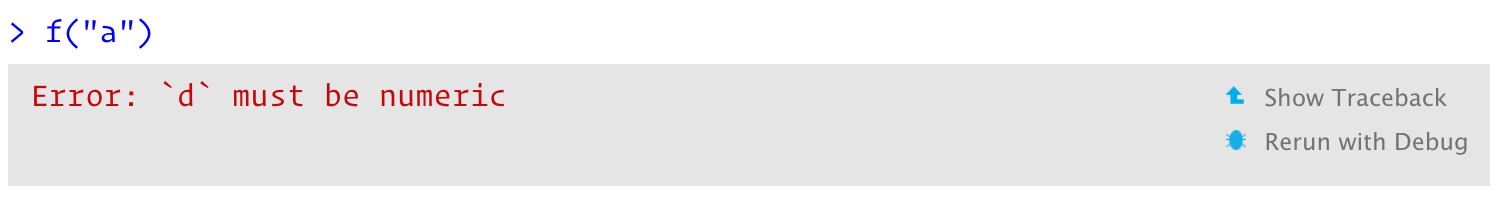
\includegraphics[width=1\linewidth]{screenshots/debugging/rstudio-error} \end{center}

Two options appear to the right of the error message: ``Show Traceback'' and ``Rerun with Debug''. If you click ``Show traceback'' you see:

\begin{center}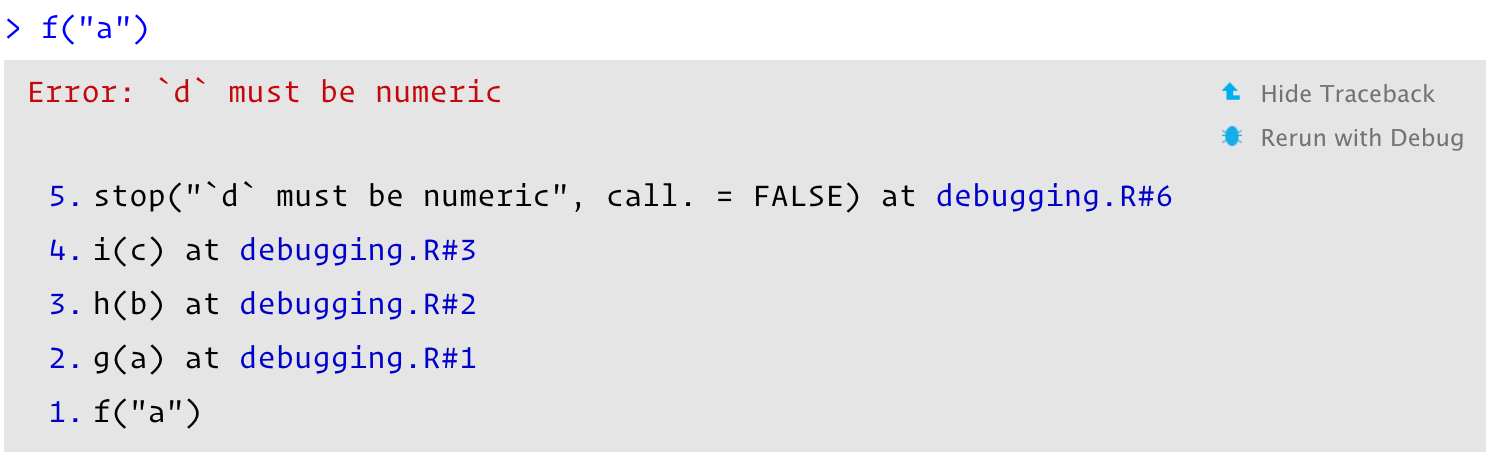
\includegraphics[width=1\linewidth]{screenshots/debugging/rstudio-traceback} \end{center}

If you're not using RStudio, you can use \texttt{traceback()} to get the same information (sans pretty formatting):

\begin{Shaded}
\begin{Highlighting}[]
\KeywordTok{traceback}\NormalTok{()}
\CommentTok{#> 5: stop("`d` must be numeric", call. = FALSE) at debugging.R#6}
\CommentTok{#> 4: i(c) at debugging.R#3}
\CommentTok{#> 3: h(b) at debugging.R#2}
\CommentTok{#> 2: g(a) at debugging.R#1}
\CommentTok{#> 1: f("a")}
\end{Highlighting}
\end{Shaded}

NB: You read the \texttt{traceback()} output from bottom to top: the initial call is \texttt{f()}, which calls \texttt{g()}, then \texttt{h()}, then \texttt{i()}, which triggers the error. If you're calling code that you \texttt{source()}d into R, the traceback will also display the location of the function, in the form \texttt{filename.r\#linenumber}. These are clickable in RStudio, and will take you to the corresponding line of code in the editor.

\hypertarget{debug-lazy}{%
\subsection{Lazy evaluation}\label{debug-lazy}}

\indexc{last\_trace()}

One drawback to \texttt{traceback()} is that it always linearises the call tree, which can be confusing if there is much lazy evaluation involved (Section \ref{lazy-call-stack}). For example, take the following example where the error happens when evaluating the first argument to \texttt{f()}:

\begin{Shaded}
\begin{Highlighting}[]
\NormalTok{j <-}\StringTok{ }\ControlFlowTok{function}\NormalTok{() }\KeywordTok{k}\NormalTok{()}
\NormalTok{k <-}\StringTok{ }\ControlFlowTok{function}\NormalTok{() }\KeywordTok{stop}\NormalTok{(}\StringTok{"Oops!"}\NormalTok{, }\DataTypeTok{call. =} \OtherTok{FALSE}\NormalTok{)}
\KeywordTok{f}\NormalTok{(}\KeywordTok{j}\NormalTok{())}
\CommentTok{#> Error: Oops!}
\end{Highlighting}
\end{Shaded}

\begin{Shaded}
\begin{Highlighting}[]
\KeywordTok{traceback}\NormalTok{()}
\CommentTok{#> 7: stop("Oops!") at #1}
\CommentTok{#> 6: k() at #1}
\CommentTok{#> 5: j() at debugging.R#1}
\CommentTok{#> 4: i(c) at debugging.R#3}
\CommentTok{#> 3: h(b) at debugging.R#2}
\CommentTok{#> 2: g(a) at debugging.R#1}
\CommentTok{#> 1: f(j())}
\end{Highlighting}
\end{Shaded}

You can using \texttt{rlang::with\_abort()} and \texttt{rlang::last\_trace()} to see the call tree. Here, I think it makes it much easier to see the source of the problem. Look at the last branch of of the call tree so see that the error comes from \texttt{j()} calling \texttt{k()}.

\begin{Shaded}
\begin{Highlighting}[]
\NormalTok{rlang}\OperatorTok{::}\KeywordTok{with_abort}\NormalTok{(}\KeywordTok{f}\NormalTok{(}\KeywordTok{j}\NormalTok{()))}
\CommentTok{#> Error: Oops!}
\NormalTok{rlang}\OperatorTok{::}\KeywordTok{last_trace}\NormalTok{()}
\CommentTok{#>     █}
\CommentTok{#>  1. ├─rlang::with_abort(f(j()))}
\CommentTok{#>  2. │ └─base::withCallingHandlers(...)}
\CommentTok{#>  3. ├─global::f(j())}
\CommentTok{#>  4. │ └─global::g(a)}
\CommentTok{#>  5. │   └─global::h(b)}
\CommentTok{#>  6. │     └─global::i(c)}
\CommentTok{#>  7. └─global::j()}
\CommentTok{#>  8.   └─global::k()}
\end{Highlighting}
\end{Shaded}

NB: \texttt{rlang::last\_trace()} is ordered in the opposite way to \texttt{traceback()}. We'll come back to that issue in Section \ref{call-stack-ordering}.

\hypertarget{browser}{%
\section{The interactive debugger}\label{browser}}

\index{debugging!interactive}
\indexc{browser()}

Sometimes, the precise location of the error is enough to let you track it down and fix it. Frequently, however, you need more information, and the easiest way to get it is with the interactive debugger which allows you to pause execution of a function and interactively explore its state.

If you're using RStudio, the easiest way to enter the interactive debugger is through RStudio's ``Rerun with Debug'' tool. This reruns the command that created the error, pausing execution where the error occurred. Otherwise, you can insert a call to \texttt{browser()} where you want to pause, and re-run the function yourself. For example, we could insert a call \texttt{browser()} in \texttt{g()}:

\begin{Shaded}
\begin{Highlighting}[]
\NormalTok{g <-}\StringTok{ }\ControlFlowTok{function}\NormalTok{(b) \{}
  \KeywordTok{browser}\NormalTok{()}
  \KeywordTok{h}\NormalTok{(b)}
\NormalTok{\}}
\KeywordTok{f}\NormalTok{(}\DecValTok{10}\NormalTok{)}
\end{Highlighting}
\end{Shaded}

\texttt{browser()} is just a regular function call which means that you can run it conditionally by wrapping it in an \texttt{if} statement:

\begin{Shaded}
\begin{Highlighting}[]
\NormalTok{g <-}\StringTok{ }\ControlFlowTok{function}\NormalTok{(b) \{}
  \ControlFlowTok{if}\NormalTok{ (b }\OperatorTok{<}\StringTok{ }\DecValTok{0}\NormalTok{) \{}
    \KeywordTok{browser}\NormalTok{()}
\NormalTok{  \}}
  \KeywordTok{h}\NormalTok{(b)}
\NormalTok{\}}
\end{Highlighting}
\end{Shaded}

In either case, you'll end up in an interactive environment \emph{inside} the function where you can run arbitrary R code to explore the current state. You'll know when you're in the interactive debugger because you get a special prompt:

\begin{verbatim}
Browse[1]> 
\end{verbatim}

In RStudio, you'll see the corresponding code in the editor (with the statement that will be run next highlighted), objects in the current environment in the ``Environment'' pane, and the call stack in the ``Traceback'' pane.

\hypertarget{browser-commands}{%
\subsection{\texorpdfstring{\texttt{browser()} commands}{browser() commands}}\label{browser-commands}}

As well as allowing you to run regular R code, \texttt{browser()} provides a few special commands. You can use them by either typing short text commands, or by clicking a button in the RStudio toolbar, Figure \ref{fig:debug-toolbar}:

\begin{figure}

{\centering 
\includegraphics[width=0.5\linewidth]{screenshots/debug-toolbar} 

}

\caption{RStudio debugging toolbar}\label{fig:debug-toolbar}
\end{figure}

\begin{itemize}
\item
  Next, \texttt{n}: executes the next step in the function. If you have a
  variable named \texttt{n}, you'll need \texttt{print(n)} to display its value.
\item
  Step into, 
\includegraphics[width=0.20833in,height=\textheight]{screenshots/step-into.png} or \texttt{s}:
  works like next, but if the next step is a function, it will step into that
  function so you can explore it interactively.
\item
  Finish, 
\includegraphics[width=0.20833in,height=\textheight]{screenshots/finish-loop.png} or \texttt{f}:
  finishes execution of the current loop or function.
\item
  Continue, \texttt{c}: leaves interactive debugging and continues regular execution
  of the function. This is useful if you've fixed the bad state and want to
  check that the function proceeds correctly.
\item
  Stop, \texttt{Q}: stops debugging, terminates the function, and returns to the global
  workspace. Use this once you've figured out where the problem is, and you're
  ready to fix it and reload the code.
\end{itemize}

There are two other slightly less useful commands that aren't available in the toolbar:

\begin{itemize}
\item
  Enter: repeats the previous command. I find this too easy to activate
  accidentally, so I turn it off using \texttt{options(browserNLdisabled\ =\ TRUE)}.
  \index{options!browserNLdisabled@\texttt{browserNLdisabled}}
\item
  \texttt{where}: prints stack trace of active calls (the interactive equivalent of
  \texttt{traceback}).
\end{itemize}

\hypertarget{alternatives}{%
\subsection{Alternatives}\label{alternatives}}

There are three alternatives to using \texttt{browser()}: setting breakpoints in RStudio, \texttt{option(error\ =\ recover)}, and \texttt{debug()} and friends.

\hypertarget{breakpoints}{%
\subsubsection{Breakpoints}\label{breakpoints}}

\index{breakpoints}

In RStudio, you can set a breakpoint by clicking to the left of the line number, or pressing \texttt{Shift\ +\ F9}. Breakpoints behave similarly to \texttt{browser()} but they are easier to set (one click instead of nine key presses), and you don't run the risk of accidentally including a \texttt{browser()} statement in your source code. There are two small downsides to breakpoints:

\begin{itemize}
\item
  There are a few unusual situations in which breakpoints will not work.
  Read \href{http://www.rstudio.com/ide/docs/debugging/breakpoint-troubleshooting}{breakpoint troubleshooting} for more details.
\item
  RStudio currently does not support conditional breakpoints.
\end{itemize}

\hypertarget{recover}{%
\subsubsection{\texorpdfstring{\texttt{recover()}}{recover()}}\label{recover}}

\index{options!error@\texttt{error}}
\indexc{recover()}

Another way to activate \texttt{browser()} is to use \texttt{options(error\ =\ recover)}. Now when you get an error, you'll get an interactive prompt that displays the traceback and gives you the ability to interactively debug inside any of the frames:

\begin{Shaded}
\begin{Highlighting}[]
\KeywordTok{options}\NormalTok{(}\DataTypeTok{error =}\NormalTok{ recover)}
\KeywordTok{f}\NormalTok{(}\StringTok{"x"}\NormalTok{)}
\CommentTok{#> Error: `d` must be numeric}
\CommentTok{#> }
\CommentTok{#> Enter a frame number, or 0 to exit   }
\CommentTok{#> }
\CommentTok{#> 1: f("x")}
\CommentTok{#> 2: debugging.R#1: g(a)}
\CommentTok{#> 3: debugging.R#2: h(b)}
\CommentTok{#> 4: debugging.R#3: i(c)}
\CommentTok{#> }
\CommentTok{#> Selection:}
\end{Highlighting}
\end{Shaded}

You can return to default error handling with \texttt{options(error\ =\ NULL)}.

\hypertarget{debug}{%
\subsubsection{\texorpdfstring{\texttt{debug()}}{debug()}}\label{debug}}

\indexc{debug()}
\indexc{trace()}
\indexc{setBreakpoint()}

Another approach is to call a function that inserts the \texttt{browser()} call for you:

\begin{itemize}
\item
  \texttt{debug()} inserts a browser statement in the first line of the specified
  function. \texttt{undebug()} removes it. Alternatively, you can use \texttt{debugonce()}
  to browse only on the next run.
\item
  \texttt{utils::setBreakpoint()} works similarly, but instead of taking a function
  name, it takes a file name and line number and finds the appropriate function
  for you.
\end{itemize}

These two functions are both special cases of \texttt{trace()}, which inserts arbitrary code at any position in an existing function. \texttt{trace()} is occasionally useful when you're debugging code that you don't have the source for. To remove tracing from a function, use \texttt{untrace()}. You can only perform one trace per function, but that one trace can call multiple functions.

\hypertarget{call-stack-ordering}{%
\subsubsection{The call stack}\label{call-stack-ordering}}

\index{call stacks}

Unfortunately, the call stacks printed by \texttt{traceback()}, \texttt{browser()} \& \texttt{where}, and \texttt{recover()} are not consistent. The following table shows how the call stacks from a simple nested set of calls are displayed by the three tools. The numbering is different between \texttt{traceback()} and \texttt{where}, and \texttt{recover()} displays calls in the opposite order.

\begin{longtable}[]{@{}llll@{}}
\toprule
\texttt{traceback()} & \texttt{where} & \texttt{recover()} & rlang functions\tabularnewline
\midrule
\endhead
\texttt{5:\ stop("...")} & & &\tabularnewline
\texttt{4:\ i(c)} & \texttt{where\ 1:\ i(c)} & \texttt{1:\ f()} & \texttt{1.\ └─global::f(10)}\tabularnewline
\texttt{3:\ h(b)} & \texttt{where\ 2:\ h(b)} & \texttt{2:\ g(a)} & \texttt{2.\ \ \ └─global::g(a)}\tabularnewline
\texttt{2:\ g(a)} & \texttt{where\ 3:\ g(a)} & \texttt{3:\ h(b)} & \texttt{3.\ \ \ \ \ └─global::h(b)}\tabularnewline
\texttt{1:\ f("a")} & \texttt{where\ 4:\ f("a")} & \texttt{4:\ i("a")} & \texttt{4.\ \ \ \ \ \ \ └─global::i("a")}\tabularnewline
\bottomrule
\end{longtable}

RStudio displays calls in the same order as \texttt{traceback()}. rlang functions use the same ordering and numbering as \texttt{recover()}, but also use indenting to reinforce the hierarchy of calls.

\hypertarget{debug-compiled}{%
\subsection{Compiled code}\label{debug-compiled}}

\index{debugging!C code}

It is also possible to use an interactive debugger (gdb or lldb) for compiled code (like C or C++). Unfortunately that's beyond the scope of this book, but there are a few resources that you might find useful:

\begin{itemize}
\tightlist
\item
  \url{http://r-pkgs.had.co.nz/src.html\#src-debugging}
\item
  \url{https://github.com/wch/r-debug/blob/master/debugging-r.md}
\item
  \url{http://kevinushey.github.io/blog/2015/04/05/debugging-with-valgrind/}
\item
  \url{https://www.jimhester.com/2018/08/22/debugging-rstudio/}
\end{itemize}

\hypertarget{non-interactive-debugging}{%
\section{Non-interactive debugging}\label{non-interactive-debugging}}

\index{debugging!non-interactive}

Debugging is most challenging when you can't run code interactively, typically because it's part of some pipeline run automatically (possibly on another computer), or because the error doesn't occur when you run same code interactively. This can be extremely frustrating!

This section will give you some useful tools, but don't forget the general strategy in Section \ref{debugging-strategy}. When you can't explore interactively, it's particularly important to spend some time making the problem as small as possible so you can iterate quickly. Sometimes \texttt{callr::r(f,\ list(1,\ 2))} can useful; this calls \texttt{f(1,\ 2)} in a fresh session, and can be a useful way to reproduce the problem.

You might also want to double check for these common issues:

\begin{itemize}
\item
  Is the global environment different? Have you loaded different packages?
  Are there objects left around from previous sessions that are causing
  differences?
\item
  Is the working directory different?
\item
  Is the \texttt{PATH} environment variable, which determines where external
  commands (like \texttt{git}) are found, different?
\item
  Is the \texttt{R\_LIBS} environment variable, which determines where \texttt{library()}
  looks for packages, different?
\end{itemize}

\hypertarget{dump.frames}{%
\subsection{\texorpdfstring{\texttt{dump.frames()}}{dump.frames()}}\label{dump.frames}}

\indexc{dump.frames()}
\indexc{recover()}

\texttt{dump.frames()} is the equivalent to \texttt{recover()} for non-interactive code; it saves a \texttt{last.dump.rda} file in the working directory. Later, an interactive session, you can later \texttt{load("last.dump.rda");\ debugger()} to enter an interactive debugger with the same interface as \texttt{recover()}. This lets you ``cheat'', interactively debugging code that was run non-interactively.

\begin{Shaded}
\begin{Highlighting}[]
\CommentTok{# In batch R process ----}
\NormalTok{dump_and_quit <-}\StringTok{ }\ControlFlowTok{function}\NormalTok{() \{}
  \CommentTok{# Save debugging info to file last.dump.rda}
  \KeywordTok{dump.frames}\NormalTok{(}\DataTypeTok{to.file =} \OtherTok{TRUE}\NormalTok{)}
  \CommentTok{# Quit R with error status}
  \KeywordTok{q}\NormalTok{(}\DataTypeTok{status =} \DecValTok{1}\NormalTok{)}
\NormalTok{\}}
\KeywordTok{options}\NormalTok{(}\DataTypeTok{error =}\NormalTok{ dump_and_quit)}

\CommentTok{# In a later interactive session ----}
\KeywordTok{load}\NormalTok{(}\StringTok{"last.dump.rda"}\NormalTok{)}
\KeywordTok{debugger}\NormalTok{()}
\end{Highlighting}
\end{Shaded}

\hypertarget{print-debugging}{%
\subsection{Print debugging}\label{print-debugging}}

\index{debugging!with print}

If \texttt{dump.frames()} doesn't help, a good fallback is \textbf{print debugging}, where you insert numerous print statements to precisely locate the problem, and see the values of important variables. Print debugging is slow and primitive, but it always works, so it's particularly useful if you can't get a good traceback. Start by inserting coarse-grained markers, and then make them progressively more fine-grained as you determine exactly where the problem is.

\begin{Shaded}
\begin{Highlighting}[]
\NormalTok{f <-}\StringTok{ }\ControlFlowTok{function}\NormalTok{(a) \{}
  \KeywordTok{cat}\NormalTok{(}\StringTok{"f()}\CharTok{\textbackslash{}n}\StringTok{"}\NormalTok{)}
  \KeywordTok{g}\NormalTok{(a)}
\NormalTok{\}}
\NormalTok{g <-}\StringTok{ }\ControlFlowTok{function}\NormalTok{(b) \{}
  \KeywordTok{cat}\NormalTok{(}\StringTok{"g()}\CharTok{\textbackslash{}n}\StringTok{"}\NormalTok{)}
  \KeywordTok{cat}\NormalTok{(}\StringTok{"b ="}\NormalTok{, b, }\StringTok{"}\CharTok{\textbackslash{}n}\StringTok{"}\NormalTok{)}
  \KeywordTok{h}\NormalTok{(b)}
\NormalTok{\}}
\NormalTok{h <-}\StringTok{ }\ControlFlowTok{function}\NormalTok{(c) \{}
  \KeywordTok{cat}\NormalTok{(}\StringTok{"i()}\CharTok{\textbackslash{}n}\StringTok{"}\NormalTok{)}
  \KeywordTok{i}\NormalTok{(c)}
\NormalTok{\}}

\KeywordTok{f}\NormalTok{(}\DecValTok{10}\NormalTok{)}
\CommentTok{#> f()}
\CommentTok{#> g()}
\CommentTok{#> b = 10 }
\CommentTok{#> i()}
\CommentTok{#> [1] 20}
\end{Highlighting}
\end{Shaded}

Print debugging is particularly useful for compiled code because it's not uncommon for the compiler to modify your code to such an extent you can't figure out the root problem even when inside an interactive debugger.

\hypertarget{rmarkdown}{%
\subsection{RMarkdown}\label{rmarkdown}}

\index{debugging!RMarkdown}

Debugging code inside RMarkdown files requires some special tools. First, if you're knitting the file using RStudio, switch to calling \texttt{rmarkdown::render("path/to/file.Rmd")} instead. This runs the code in the current session, which makes it easier to debug. If doing this makes the problem go away, you'll need to figure out what makes the environments different.

If the problem persists, you'll need to use your interactive debugging skills. Whatever method you use, you'll need an extra step: in the error handler, you'll need to call \texttt{sink()}. This removes the default ``sink'' that knitr uses to capture all output, and ensures that you can see the results in the console. For example, to use \texttt{recover()} with RMarkdown, you'd put the following code in your setup block:

\begin{Shaded}
\begin{Highlighting}[]
\KeywordTok{options}\NormalTok{(}\DataTypeTok{error =} \ControlFlowTok{function}\NormalTok{() \{}
  \KeywordTok{sink}\NormalTok{()}
  \KeywordTok{recover}\NormalTok{()}
\NormalTok{\})}
\end{Highlighting}
\end{Shaded}

This will generate a warning about ``no sink to remove'' when knitr completes; you can safely ignore this warning.

If you simply want to a traceback, the easiest option is to use \texttt{rlang::trace\_back()}, taking advantage of the \texttt{rlang\_trace\_top\_env} option. This ensures that you only see the traceback from your code, not all of the functions called by RMarkdown and knitr.

\begin{Shaded}
\begin{Highlighting}[]
\KeywordTok{options}\NormalTok{(}\DataTypeTok{rlang_trace_top_env =}\NormalTok{ rlang}\OperatorTok{::}\KeywordTok{current_env}\NormalTok{())}
\KeywordTok{options}\NormalTok{(}\DataTypeTok{error =} \ControlFlowTok{function}\NormalTok{() \{}
  \KeywordTok{sink}\NormalTok{()}
  \KeywordTok{print}\NormalTok{(rlang}\OperatorTok{::}\KeywordTok{trace_back}\NormalTok{(}\DataTypeTok{bottom =} \KeywordTok{sys.frame}\NormalTok{(}\OperatorTok{-}\DecValTok{1}\NormalTok{)), }\DataTypeTok{simplify =} \StringTok{"none"}\NormalTok{)}
\NormalTok{\})}
\end{Highlighting}
\end{Shaded}

\hypertarget{non-error-failures}{%
\section{Non-error failures}\label{non-error-failures}}

\index{debugging!warnings}
\index{debugging!messages}
\index{debugging!crashes}
\index{crashes|see {debugging}}

There are other ways for a function to fail apart from throwing an error:

\begin{itemize}
\item
  A function may generate an unexpected warning. The easiest way to track down
  warnings is to convert them into errors with \texttt{options(warn\ =\ 2)} and use the
  in the call stack, like \texttt{doWithOneRestart()}, \texttt{withOneRestart()},
  regular debugging tools. When you do this you'll see some extra calls
  \texttt{withRestarts()}, and \texttt{.signalSimpleWarning()}. Ignore these: they are
  internal functions used to turn warnings into errors.
\item
  A function may generate an unexpected message. You can use
  \texttt{rlang::with\_abort()} to turn these messages into errors:

\begin{Shaded}
\begin{Highlighting}[]
\NormalTok{f <-}\StringTok{ }\ControlFlowTok{function}\NormalTok{() }\KeywordTok{g}\NormalTok{()}
\NormalTok{g <-}\StringTok{ }\ControlFlowTok{function}\NormalTok{() }\KeywordTok{message}\NormalTok{(}\StringTok{"Hi!"}\NormalTok{)}
\KeywordTok{f}\NormalTok{()}
\CommentTok{#> Hi!}

\NormalTok{rlang}\OperatorTok{::}\KeywordTok{with_abort}\NormalTok{(}\KeywordTok{f}\NormalTok{(), }\StringTok{"message"}\NormalTok{)}
\CommentTok{#> Error: Hi!}
\NormalTok{rlang}\OperatorTok{::}\KeywordTok{last_trace}\NormalTok{()}
\CommentTok{#>     █}
\CommentTok{#>  1. ├─rlang::with_abort(f(), "message")}
\CommentTok{#>  2. │ └─base::withCallingHandlers(...)}
\CommentTok{#>  3. └─global::f()}
\CommentTok{#>  4.   └─global::g()}
\end{Highlighting}
\end{Shaded}
\item
  A function might never return. This is particularly hard to debug
  automatically, but sometimes terminating the function and looking at the
  \texttt{traceback()} is informative. Otherwise, use use print debugging,
  as in Section \ref{print-debugging}.
\item
  The worst scenario is that your code might crash R completely, leaving you
  with no way to interactively debug your code. This indicates a bug in
  compiled (C or C++) code.

  If it's in your compiled code, you'll need to follow the links in Section
  \ref{debug-compiled} and learn how to use an interactive C debugger
  (or insert many print statements).

  If it's in a package or base R, you'll need to contact the package
  maintainer. In either case, work on making the smallest possible
  reprex (Section \ref{getting-help}) to help the developer help you.
\end{itemize}

\hypertarget{perf-measure}{%
\chapter{Measuring performance}\label{perf-measure}}

\index{performance!measuring}

\hypertarget{introduction-8}{%
\section{Introduction}\label{introduction-8}}

\begin{quote}
``Programmers waste enormous amounts of time thinking about, or worrying
about, the speed of noncritical parts of their programs, and these attempts
at efficiency actually have a strong negative impact when debugging and
maintenance are considered.''

\hspace*{\fill} --- Donald Knuth.
\end{quote}

Before you can make your code faster, you first need to figure out what's making it slow. This sounds easy, but it's not. Even experienced programmers have a hard time identifying bottlenecks in their code. So instead of relying on your intuition, you should \textbf{profile} your code: measure the run-time of each line of code using realistic inputs.

Once you've identified bottlenecks you'll need to carefully experiment with alternatives to find faster code that is still equivalent. In Chapter \ref{perf-improve} you'll learn a bunch of ways to speed up code, but first you need to learn how to \textbf{microbenchmark} so that you can precisely measure the difference in performance.

\hypertarget{outline-6}{%
\subsection*{Outline}\label{outline-6}}
\addcontentsline{toc}{subsection}{Outline}

\begin{itemize}
\item
  Section \ref{profiling} shows you how to use profiling tools to dig into
  exactly what is making code slow.
\item
  Section \ref{microbenchmarking} shows how to use microbenchmarking to
  explore alternative implementations and figure out exactly which one is
  fastest.
\end{itemize}

\hypertarget{prerequisites-5}{%
\subsection*{Prerequisites}\label{prerequisites-5}}
\addcontentsline{toc}{subsection}{Prerequisites}

We'll use \href{https://rstudio.github.io/profvis/}{profvis} for profiling, and \href{https://bench.r-lib.org/}{bench} for microbenchmarking.

\begin{Shaded}
\begin{Highlighting}[]
\KeywordTok{library}\NormalTok{(profvis)}
\KeywordTok{library}\NormalTok{(bench)}
\end{Highlighting}
\end{Shaded}

\hypertarget{profiling}{%
\section{Profiling}\label{profiling}}

\index{profiling}
\indexc{RProf()}

Across programming languages, the primary tool used to understand code performance is the profiler. There are a number of different types of profilers ,but R uses a fairly simple type called a sampling or statistical profiler. A sampling profiler stops the execution of code every few milliseconds and records the call stack (i.e.~which function is currently executing, and the funcion that function, and so on). For example, consider \texttt{f()}, below:

\begin{Shaded}
\begin{Highlighting}[]
\NormalTok{f <-}\StringTok{ }\ControlFlowTok{function}\NormalTok{() \{}
  \KeywordTok{pause}\NormalTok{(}\FloatTok{0.1}\NormalTok{)}
  \KeywordTok{g}\NormalTok{()}
  \KeywordTok{h}\NormalTok{()}
\NormalTok{\}}
\NormalTok{g <-}\StringTok{ }\ControlFlowTok{function}\NormalTok{() \{}
  \KeywordTok{pause}\NormalTok{(}\FloatTok{0.1}\NormalTok{)}
  \KeywordTok{h}\NormalTok{()}
\NormalTok{\}}
\NormalTok{h <-}\StringTok{ }\ControlFlowTok{function}\NormalTok{() \{}
  \KeywordTok{pause}\NormalTok{(}\FloatTok{0.1}\NormalTok{)}
\NormalTok{\}}
\end{Highlighting}
\end{Shaded}

(I use \texttt{profvis::pause()} instead of \texttt{Sys.sleep()} because \texttt{Sys.sleep()} does not appear in profiling outputs because as far as R can tell, it doesn't use up any computing time.) \indexc{pause()}

If we profiled the execution of \texttt{f()}, stopping the execution of code every 0.1 s, we'd see a profile like this:

\begin{Shaded}
\begin{Highlighting}[]
\StringTok{"pause"} \StringTok{"f"} 
\StringTok{"pause"} \StringTok{"f"} \StringTok{"g"}
\StringTok{"pause"} \StringTok{"f"} \StringTok{"g"} \StringTok{"h"}
\StringTok{"pause"} \StringTok{"f"} \StringTok{"h"}
\end{Highlighting}
\end{Shaded}

Each line represents one ``tick'' of the profiler (0.1 s in this case), and function calls are recorded from right to left: the first line shows \texttt{f()} calling \texttt{pause()}. It shows that the code spends 0.1 s running \texttt{f()}, then 0.2 s running \texttt{g()}, then 0.1 s running \texttt{h()}.

If we actually profile \texttt{f()}, using \texttt{utils::Rprof()} as in the code below, we're unlikely to get such a clear result.

\begin{Shaded}
\begin{Highlighting}[]
\NormalTok{tmp <-}\StringTok{ }\KeywordTok{tempfile}\NormalTok{()}
\KeywordTok{Rprof}\NormalTok{(tmp, }\DataTypeTok{interval =} \FloatTok{0.1}\NormalTok{)}
\KeywordTok{f}\NormalTok{()}
\KeywordTok{Rprof}\NormalTok{(}\OtherTok{NULL}\NormalTok{)}
\KeywordTok{writeLines}\NormalTok{(}\KeywordTok{readLines}\NormalTok{(tmp))}
\CommentTok{#> sample.interval=100000}
\CommentTok{#> "pause" "g" "f" }
\CommentTok{#> "pause" "h" "g" "f" }
\CommentTok{#> "pause" "h" "f" }
\end{Highlighting}
\end{Shaded}

That's because all profilers must make a fundamental trade-off between accuracy and performance. The compromise that makes, using a sampling profiler, only has minimal impact on performance, but is fundamentally stochastic because there's some variability in both the accuracy of the timer and in the time taken by each operation. That means each time that you profile you'll get a slightly different answer. Fortunately, the variability most affects functions that take very little time ot run, which are also the functions that we're least interested in.

\hypertarget{visualising-profiles}{%
\subsection{Visualising profiles}\label{visualising-profiles}}

\indexc{profvis()}

The default profiling resolution is quite small, so if your function takes even a few seconds it will generate hundreds of samples. That quickly grows beyond our ability to look at directly, so instead of using \texttt{uils::Rprof()} we'll use the profvis package to visualise aggregates. profvis also connects profiling data back to the underlying source code, making it easier to build up a mental model of what you need to change. If you find profvis doesn't help for your code, you might try one of the other options like \texttt{utils::summaryRprof()} or the proftools package (Tierney and Jarjour \protect\hyperlink{ref-proftools}{2016}).

There are two ways to use profvis:

\begin{itemize}
\item
  From the ``Profile'' menu in RStudio.
\item
  With \texttt{profvis::profvis()}. I recommend storing your code in a separate
  file and \texttt{source()}ing it in; this will ensure you get the best connection
  between profiling data and source code.

\begin{Shaded}
\begin{Highlighting}[]
\KeywordTok{source}\NormalTok{(}\StringTok{"profiling-example.R"}\NormalTok{)}
\KeywordTok{profvis}\NormalTok{(}\KeywordTok{f}\NormalTok{())}
\end{Highlighting}
\end{Shaded}
\end{itemize}

After profiling is complete, profvis will open an interactive HTML document that allows you to explore the results. There are two panes, as shown in Figure \ref{fig:flamegraph}.

\begin{figure}

{\centering 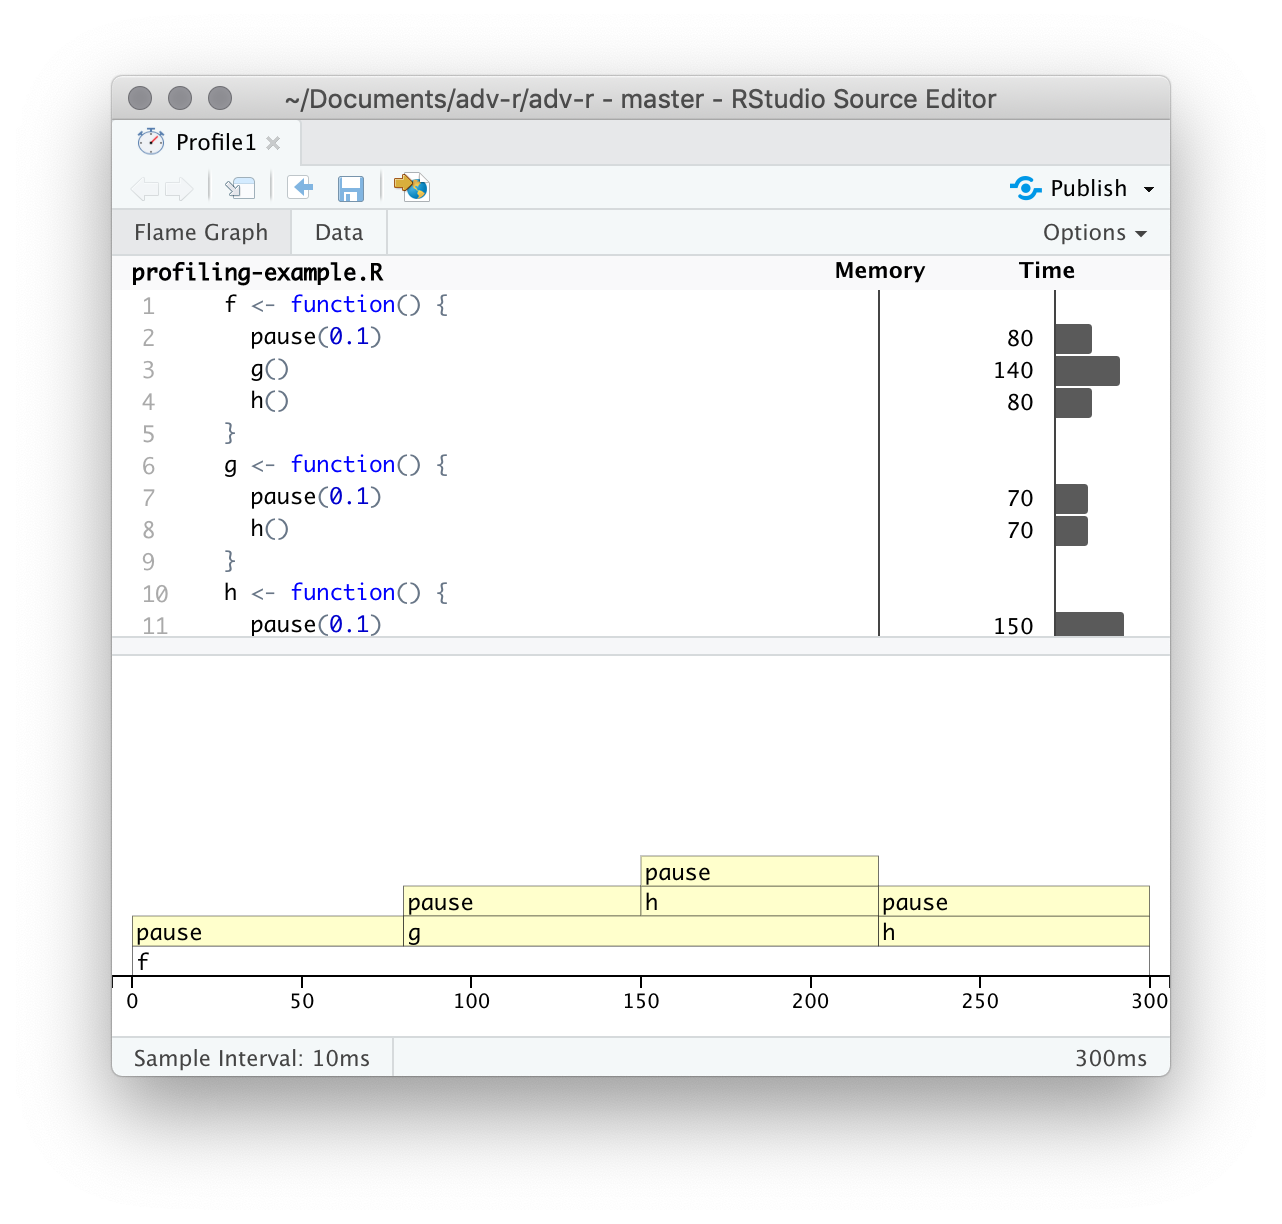
\includegraphics[width=1\linewidth]{screenshots/performance/flamegraph} 

}

\caption{profvis output showing source on top and flame graph below.}\label{fig:flamegraph}
\end{figure}

The top pane shows the source code, overlaid with bar graphs for memory and execution time for each line of code. Here I'll focus on time, and we'll come back to memory shortly. This display gives you a good overall feel for the bottlenecks but doesn't always help you precisely identify the cause. Here, for example, you can see that \texttt{h()} takes 150ms, twice as long as \texttt{g()}; that's not because the function itself is slower, but because it's called twice as often.

The bottom pane displays a \textbf{flame graph} showing the full call stack. This allows you to see the full sequence of calls leading to each function, allowing you to see that \texttt{h()} is called from two different places. In this display you can mouse over individual calls to get more information, and see the corresponding line of source code, as in Figure \ref{fig:perf-info}.

\begin{figure}

{\centering 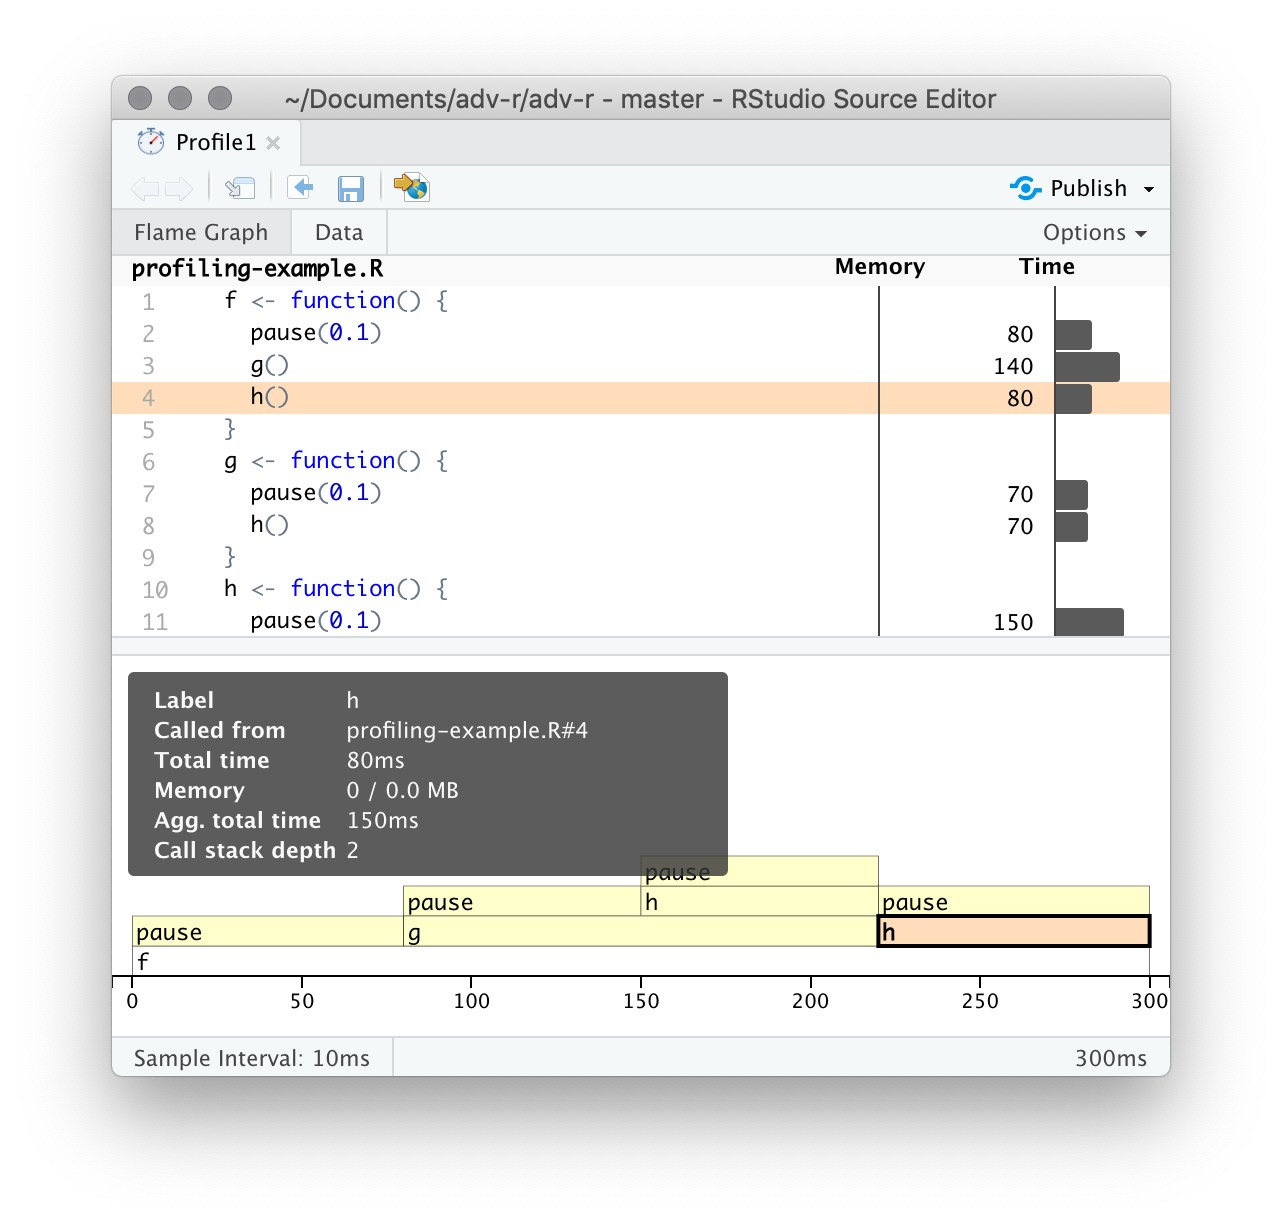
\includegraphics[width=1\linewidth]{screenshots/performance/info} 

}

\caption{Hovering over a call in the flamegraph highlights the corresponding line of code, and displays additional information about performance.}\label{fig:perf-info}
\end{figure}

Alternatively, you can use the \textbf{data tab}, Figure \ref{fig:perf-tree} lets you interactively dive into the tree of performance data. This is basically the same display as the flame graph (rotated 90°), but it's more useful when you have very large or deeply nested call stacks because you can choose to interactively zoom into only selected components.

\begin{figure}

{\centering 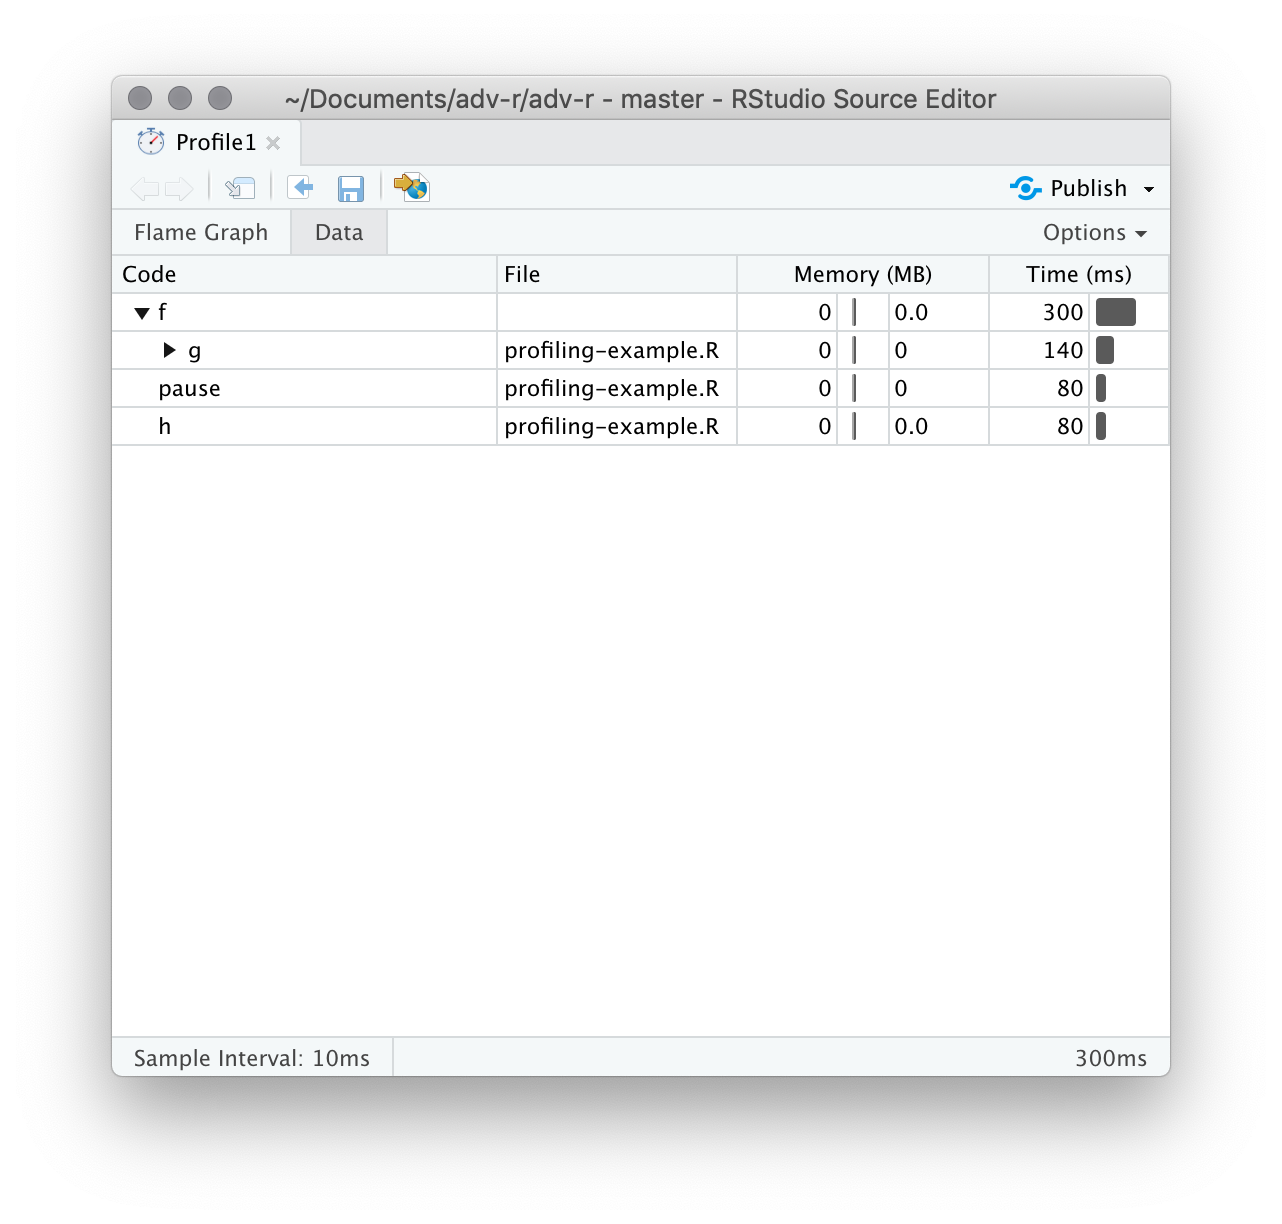
\includegraphics[width=1\linewidth]{screenshots/performance/tree} 

}

\caption{The data gives an interactive tree that allows you to selectively zoom into key components}\label{fig:perf-tree}
\end{figure}

\hypertarget{memory-profiling}{%
\subsection{Memory profiling}\label{memory-profiling}}

\index{profiling!memory}
\index{garbage collector!performance}
\index{memory usage}

There is a special entry in the flame graph that doesn't correspond to your code: \texttt{\textless{}GC\textgreater{}}, which indicates that the garbage collector is running. If \texttt{\textless{}GC\textgreater{}} is taking a lot of time, it's usually an indicating that you're creating many short-lived objects. For example, take this small snippet of code:

\begin{Shaded}
\begin{Highlighting}[]
\NormalTok{x <-}\StringTok{ }\KeywordTok{integer}\NormalTok{()}
\ControlFlowTok{for}\NormalTok{ (i }\ControlFlowTok{in} \DecValTok{1}\OperatorTok{:}\FloatTok{1e4}\NormalTok{) \{}
\NormalTok{  x <-}\StringTok{ }\KeywordTok{c}\NormalTok{(x, i)}
\NormalTok{\}}
\end{Highlighting}
\end{Shaded}

If you profile it, you'll see that most of the time is spent in the garbage collector, Figure \ref{fig:perf-memory}.

\begin{figure}

{\centering 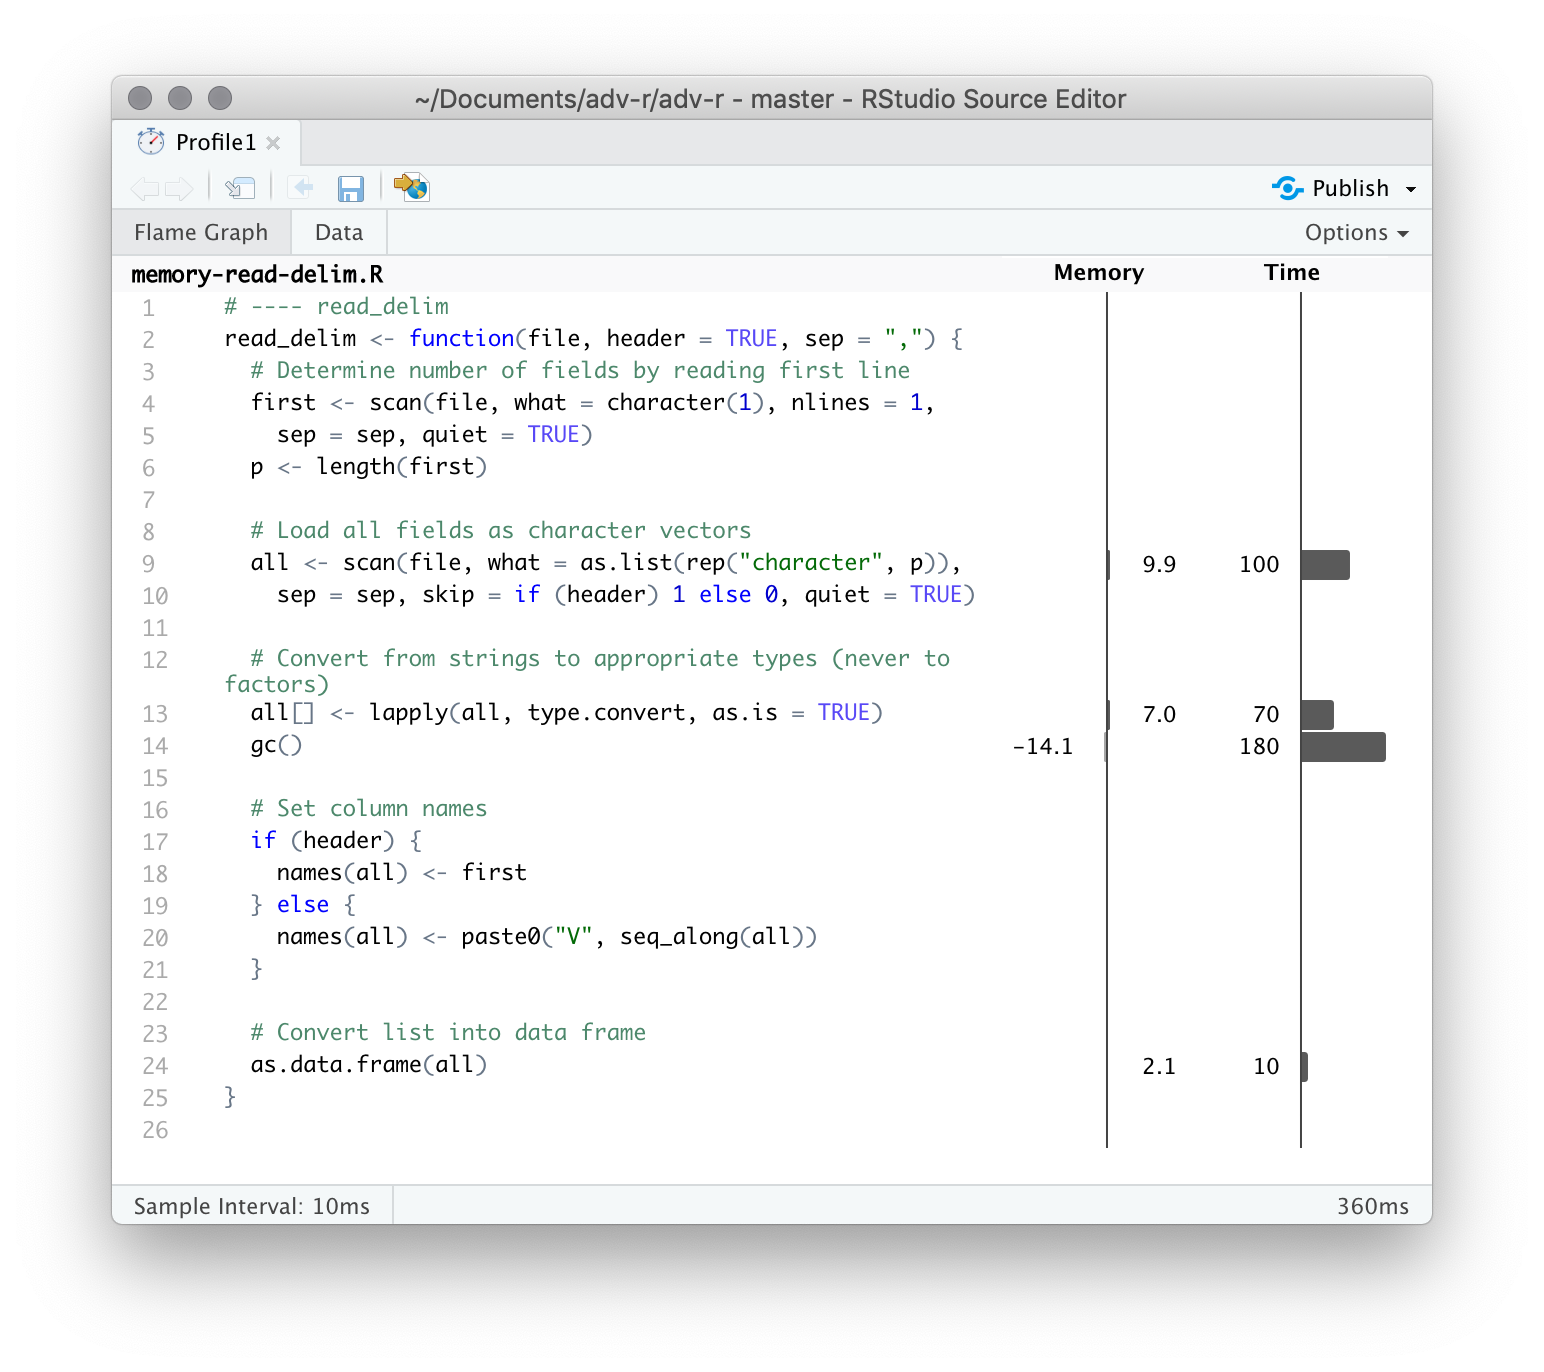
\includegraphics[width=1\linewidth]{screenshots/performance/memory} 

}

\caption{Profiling a loop that modifies an existing variable reveals that most time is spent in the garbage collector (`<GC>`)}\label{fig:perf-memory}
\end{figure}

When you see the garbage collector taking up a lot of time in your own code, you can often figure out the source of the problem by looking at the memory column: you'll see a line where large amounts of memory are being allocated (the bar on the right) and freed (the bar on the left). Here the problem arises because of copy-on-modify (Section \ref{copy-on-modify}): each iteration of the loop creates another copy of \texttt{x}. You'll learn strategies to resolve this type of problem in Section \ref{avoid-copies}.

\hypertarget{limitations}{%
\subsection{Limitations}\label{limitations}}

\index{profiling!limitations}

There are some other limitations to profiling:

\begin{itemize}
\item
  Profiling does not extend to C code. You can see if your R code calls C/C++
  code but not what functions are called inside of your C/C++ code.
  Unfortunately, tools for profiling compiled code are beyond the scope of
  this book; start by looking at \url{https://github.com/r-prof/jointprof}.
\item
  If you're doing a lot of functional programming with anonymous functions,
  it can be hard to figure out exactly which function is being called.
  The easiest way to work around this is to name your functions.
\item
  Lazy evaluation means that arguments are often evaluated inside another
  function, and this complicates the call stack (Section
  \ref{lazy-call-stack}). Unfortunately R's profiler doesn't store enough
  information to disentangle lazy evaluation so that in the following code,
  profiling would make it seem like \texttt{i()} was called by \texttt{j()} because the
  argument isn't evaluated until it's needed by \texttt{j()}.

\begin{Shaded}
\begin{Highlighting}[]
\NormalTok{i <-}\StringTok{ }\ControlFlowTok{function}\NormalTok{() \{}
  \KeywordTok{pause}\NormalTok{(}\FloatTok{0.1}\NormalTok{)}
  \DecValTok{10}
\NormalTok{\}}
\NormalTok{j <-}\StringTok{ }\ControlFlowTok{function}\NormalTok{(x) \{}
\NormalTok{  x }\OperatorTok{+}\StringTok{ }\DecValTok{10}
\NormalTok{\}}
\KeywordTok{j}\NormalTok{(}\KeywordTok{i}\NormalTok{())}
\end{Highlighting}
\end{Shaded}

  If this is confusing, use \texttt{force()} (Section @ref\{forcing-evaluation\}) to
  force computation to happen earlier.
\end{itemize}

\hypertarget{exercises-16}{%
\subsection{Exercises}\label{exercises-16}}

\begin{enumerate}
\def\labelenumi{\arabic{enumi}.}
\item
  Profile the following function with \texttt{torture\ =\ TRUE}. What is
  surprising? Read the source code of \texttt{rm()} to figure out what's going on.

\begin{Shaded}
\begin{Highlighting}[]
\NormalTok{f <-}\StringTok{ }\ControlFlowTok{function}\NormalTok{(}\DataTypeTok{n =} \FloatTok{1e5}\NormalTok{) \{}
\NormalTok{  x <-}\StringTok{ }\KeywordTok{rep}\NormalTok{(}\DecValTok{1}\NormalTok{, n)}
  \KeywordTok{rm}\NormalTok{(x)}
\NormalTok{\}}
\end{Highlighting}
\end{Shaded}
\end{enumerate}

\hypertarget{microbenchmarking}{%
\section{Microbenchmarking}\label{microbenchmarking}}

\index{microbenchmarking|see {benchmarking}}
\index{benchmarking}

A \textbf{microbenchmark} is a measurement of the performance of a very small piece of code, something that might take milliseconds (ms), microseconds (µs), or nanoseconds (ns) to run. Microbenchmarks are useful for comparing small snippets of code for specific tasks. Be very wary of generalising the results of microbenchmarks to real code: the observed differences in microbenchmarks will typically be dominated by higher-order effects in real code; a deep understanding of subatomic physics is not very helpful when baking.

A great tool for microbenchmarking in R is the bench package (Hester \protect\hyperlink{ref-bench}{2018}). bench uses a a high precision timer, making it possible to compare operations that only take a tiny amount of time. For example, the following code compares the speed of two approaches to computing a square root.

\begin{Shaded}
\begin{Highlighting}[]
\NormalTok{x <-}\StringTok{ }\KeywordTok{runif}\NormalTok{(}\DecValTok{100}\NormalTok{)}
\NormalTok{(lb <-}\StringTok{ }\NormalTok{bench}\OperatorTok{::}\KeywordTok{mark}\NormalTok{(}
  \KeywordTok{sqrt}\NormalTok{(x),}
\NormalTok{  x }\OperatorTok{^}\StringTok{ }\FloatTok{0.5}
\NormalTok{))}
\CommentTok{#> # A tibble: 2 x 10}
\CommentTok{#>   expression      min    mean   median     max `itr/sec` mem_alloc}
\CommentTok{#>   <chr>      <bch:tm> <bch:t> <bch:tm> <bch:t>     <dbl> <bch:byt>}
\CommentTok{#> 1 sqrt(x)    584.06ns  1.11µs 983.01ns  34.5µs   901308.      848B}
\CommentTok{#> 2 x^0.5        9.04µs 10.32µs   9.46µs 832.2µs    96858.      848B}
\CommentTok{#> # … with 3 more variables: n_gc <dbl>, n_itr <int>,}
\CommentTok{#> #   total_time <bch:tm>}
\end{Highlighting}
\end{Shaded}

By default, \texttt{bench::mark()} runs each expression at least once (\texttt{min\_iterations\ =\ 1}), and at most enough times to take 0.5s (\texttt{min\_time\ =\ 0.5}). It checks that each run returns the same value which is typically what you when microbenchmarking; if you want to compare the speed of expressions that return different values, set \texttt{check\ =\ FALSE}.

\hypertarget{benchmark-results}{%
\subsection{\texorpdfstring{\texttt{bench::mark()} results}{bench::mark() results}}\label{benchmark-results}}

\indexc{mark()}

\texttt{bench::mark()} returns the results as a tibble, with one row for each input expression, and the following columns:

\begin{itemize}
\item
  \texttt{min}, \texttt{mean}, \texttt{median}, \texttt{max}, and \texttt{itr/sec} summarise the time taken by the
  expression. Focus on the minimum (the best possible running time) and the
  median (the typical time). In this example, you can see that using the
  special purpose \texttt{sqrt()} function is faster than the general exponentiation
  operator.

  You can visualise the distribution of the individual timings with \texttt{plot()}:

\begin{Shaded}
\begin{Highlighting}[]
\KeywordTok{plot}\NormalTok{(lb)}
\end{Highlighting}
\end{Shaded}

  \begin{center}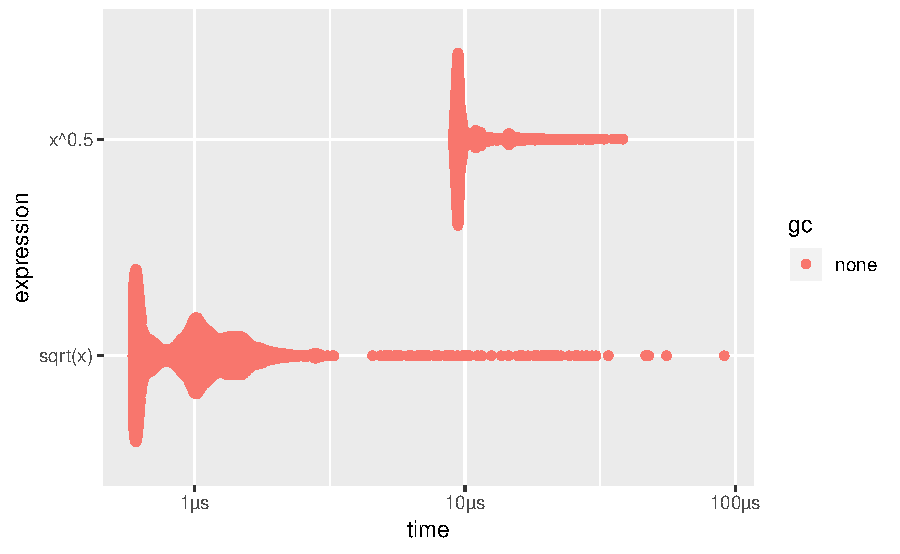
\includegraphics[width=0.7\linewidth]{Perf-measure_files/figure-latex/unnamed-chunk-9-1} \end{center}

  The distribution tends to be heavily right-skewed (note that the x-axis is
  already on a log scale!), which is why you should avoid comparing means.
  You'll also often see multimodality because your computer is running
  something else in the background.
\item
  \texttt{mem\_alloc} tells you the amount of memory allocated by the first run,
  and \texttt{n\_gc()} tells you the total number of garbage collections over all
  runs. These are useful for assessing the memory usage of the expression.
\item
  \texttt{n\_itr} and \texttt{total\_time} tells you how many times the expression was
  evaluated and how long that took in total. \texttt{n\_itr} will always be
  greater than the \texttt{min\_iteration} parameter, and \texttt{total\_time} will always
  be greater than the \texttt{min\_time} parameter.
\item
  \texttt{result}, \texttt{memory}, \texttt{time}, and \texttt{gc} are list-columns that store the
  raw underlying data.
\end{itemize}

Because the result is a special type of tibble, you can use \texttt{{[}} to select just the most important columns. I'll do that frequently in the next chapter.

\begin{Shaded}
\begin{Highlighting}[]
\NormalTok{lb[}\KeywordTok{c}\NormalTok{(}\StringTok{"expression"}\NormalTok{, }\StringTok{"min"}\NormalTok{, }\StringTok{"median"}\NormalTok{, }\StringTok{"itr/sec"}\NormalTok{, }\StringTok{"n_gc"}\NormalTok{)]}
\CommentTok{#> # A tibble: 2 x 5}
\CommentTok{#>   expression      min   median `itr/sec`  n_gc}
\CommentTok{#>   <chr>      <bch:tm> <bch:tm>     <dbl> <dbl>}
\CommentTok{#> 1 sqrt(x)    584.06ns 983.01ns   901308.     0}
\CommentTok{#> 2 x^0.5        9.04µs   9.46µs    96858.     0}
\end{Highlighting}
\end{Shaded}

\hypertarget{interpreting-results}{%
\subsection{Interpreting results}\label{interpreting-results}}

As with all microbenchmarks, pay careful attention to the units: here, each computation takes about 580 ns, 580 billionths of a second. To help calibrate the impact of a microbenchmark on run time, it's useful to think about how many times a function needs to run before it takes a second. If a microbenchmark takes:

\begin{itemize}
\tightlist
\item
  1 ms, then one thousand calls takes a second.
\item
  1 µs, then one million calls takes a second.
\item
  1 ns, then one billion calls takes a second.
\end{itemize}

The \texttt{sqrt()} function takes about 580 ns, or 0.58 µs, to compute the square root of 100 numbers. That means if you repeated the operation a million times, it would take 0.58 s, and hence changing the way you compute the square root is unlikely to significantly affect real code. This is the reason you need to exercise care when generalising microbenchmarking results.

\hypertarget{exercises-17}{%
\subsection{Exercises}\label{exercises-17}}

\begin{enumerate}
\def\labelenumi{\arabic{enumi}.}
\item
  Instead of using \texttt{bench::mark()}, you could use the built-in function
  \texttt{system.time()}. But \texttt{system.time()} is much less precise, so you'll
  need to repeat each operation many times with a loop, and then divide
  to find the average time of each operation, as in the code below.

\begin{Shaded}
\begin{Highlighting}[]
\NormalTok{n <-}\StringTok{ }\FloatTok{1e6}
\KeywordTok{system.time}\NormalTok{(}\ControlFlowTok{for}\NormalTok{ (i }\ControlFlowTok{in} \DecValTok{1}\OperatorTok{:}\NormalTok{n) }\KeywordTok{sqrt}\NormalTok{(x)) }\OperatorTok{/}\StringTok{ }\NormalTok{n}
\KeywordTok{system.time}\NormalTok{(}\ControlFlowTok{for}\NormalTok{ (i }\ControlFlowTok{in} \DecValTok{1}\OperatorTok{:}\NormalTok{n) x }\OperatorTok{^}\StringTok{ }\FloatTok{0.5}\NormalTok{) }\OperatorTok{/}\StringTok{ }\NormalTok{n}
\end{Highlighting}
\end{Shaded}

  How do the estimates from \texttt{system.time()} compare to those from
  \texttt{bench::mark()}? Why are they different?
\item
  Here are two other ways to compute the square root of a vector. Which
  do you think will be fastest? Which will be slowest? Use microbenchmarking
  to test your answers.

\begin{Shaded}
\begin{Highlighting}[]
\NormalTok{x }\OperatorTok{^}\StringTok{ }\NormalTok{(}\DecValTok{1} \OperatorTok{/}\StringTok{ }\DecValTok{2}\NormalTok{)}
\KeywordTok{exp}\NormalTok{(}\KeywordTok{log}\NormalTok{(x) }\OperatorTok{/}\StringTok{ }\DecValTok{2}\NormalTok{)}
\end{Highlighting}
\end{Shaded}
\end{enumerate}

\hypertarget{perf-improve}{%
\chapter{Improving performance}\label{perf-improve}}

\hypertarget{introduction-9}{%
\section{Introduction}\label{introduction-9}}

\index{performance!improving}

\begin{quote}
``We should forget about small efficiencies, say about 97\% of the time:
premature optimization is the root of all evil. Yet we should not pass up our
opportunities in that critical 3\%. A good programmer will not be lulled
into complacency by such reasoning, he will be wise to look carefully at
the critical code; but only after that code has been identified.''

\hspace*{\fill} --- Donald Knuth.
\end{quote}

Once you've used profiling to identify a bottleneck, you need to make it faster. It's difficult to provide general advice on improving performance, but I try my best with four techniques that can be applied in many situations. I'll also suggest a general strategy for performance optimisation that helps ensure that your faster code is still correct.

It's easy to get caught up in trying to remove all bottlenecks. Don't! Your time is valuable and is better spent analysing your data, not eliminating possible inefficiencies in your code. Be pragmatic: don't spend hours of your time to save seconds of computer time. To enforce this advice, you should set a goal time for your code and optimise only up to that goal. This means you will not eliminate all bottlenecks. Some you will not get to because you've met your goal. Others you may need to pass over and accept either because there is no quick and easy solution or because the code is already well optimised and no significant improvement is possible. Accept these possibilities and move on to the next candidate.

If you'd like to learn more about the performance characteristics of the R language itself, I'd highly recommend ``Evaluating the Design of the R Language'' (Morandat et al. \protect\hyperlink{ref-r-design}{2012}). It draws conclusions by combining a modified R interpreter with a wide set of code found in the wild.

\hypertarget{outline-7}{%
\subsection*{Outline}\label{outline-7}}
\addcontentsline{toc}{subsection}{Outline}

\begin{itemize}
\item
  Section \ref{code-organisation} teaches you how to organise
  your code to make optimisation as easy, and bug free, as possible.
\item
  Section \ref{already-solved} reminds you to look for existing
  solutions.
\item
  Section \ref{be-lazy} emphasises the importance of
  being lazy: often the easiest way to make a function faster is to
  let it to do less work.
\item
  Section \ref{vectorise} concisely defines vectorisation, and shows you
  how to make the most of built-in functions.
\item
  Section \ref{avoid-copies} discusses the performance perils of
  copying data.
\item
  Section \ref{t-test} pulls all the pieces together into a case
  study showing how to speed up repeated t-tests by \textasciitilde{}1000x.
\item
  Section \ref{more-techniques} finishes the chapter with pointers to
  more resources that will help you write fast code.
\end{itemize}

\hypertarget{prerequisites-6}{%
\subsection*{Prerequisites}\label{prerequisites-6}}
\addcontentsline{toc}{subsection}{Prerequisites}

We'll use \href{https://bench.r-lib.org/}{bench} to precisely compare the performance of small self-contained code chunks.

\begin{Shaded}
\begin{Highlighting}[]
\KeywordTok{library}\NormalTok{(bench)}
\end{Highlighting}
\end{Shaded}

\hypertarget{code-organisation}{%
\section{Code organisation}\label{code-organisation}}

\index{performance!strategy}

There are two traps that are easy to fall into when trying to make your code faster:

\begin{enumerate}
\def\labelenumi{\arabic{enumi}.}
\tightlist
\item
  Writing faster but incorrect code.
\item
  Writing code that you think is faster, but is actually no better.
\end{enumerate}

The strategy outlined below will help you avoid these pitfalls.

When tackling a bottleneck, you're likely to come up with multiple approaches. Write a function for each approach, encapsulating all relevant behaviour. This makes it easier to check that each approach returns the correct result and to time how long it takes to run. To demonstrate the strategy, I'll compare two approaches for computing the mean:

\begin{Shaded}
\begin{Highlighting}[]
\NormalTok{mean1 <-}\StringTok{ }\ControlFlowTok{function}\NormalTok{(x) }\KeywordTok{mean}\NormalTok{(x)}
\NormalTok{mean2 <-}\StringTok{ }\ControlFlowTok{function}\NormalTok{(x) }\KeywordTok{sum}\NormalTok{(x) }\OperatorTok{/}\StringTok{ }\KeywordTok{length}\NormalTok{(x)}
\end{Highlighting}
\end{Shaded}

I recommend that you keep a record of everything you try, even the failures. If a similar problem occurs in the future, it'll be useful to see everything you've tried. To do this I recommend RMarkdown, which makes it easy to intermingle code with detailed comments and notes.

Next, generate a representative test case. The case should be big enough to capture the essence of your problem but small enough that it only a few seconds at most. You don't want it to take too long because you'll need to run the test case many times to compare approaches. On the other hand, you don't want the case to be too small because then results might not scale up to the real problem. Hre I'm going to use 100,000 numbers:

\begin{Shaded}
\begin{Highlighting}[]
\NormalTok{x <-}\StringTok{ }\KeywordTok{runif}\NormalTok{(}\FloatTok{1e5}\NormalTok{)}
\end{Highlighting}
\end{Shaded}

Now use \texttt{bench::mark()} to precisely compare the variations. \texttt{bench::mark()} automatically checks that all calls return the same values. This doesn't guarantee that the function behaves the same for all inputs, so in an ideal world you'll also have unit tests to make sure you don't accidentally change the behaviour of the function.

\begin{Shaded}
\begin{Highlighting}[]
\NormalTok{bench}\OperatorTok{::}\KeywordTok{mark}\NormalTok{(}
  \KeywordTok{mean1}\NormalTok{(x),}
  \KeywordTok{mean2}\NormalTok{(x)}
\NormalTok{)[}\KeywordTok{c}\NormalTok{(}\StringTok{"expression"}\NormalTok{, }\StringTok{"min"}\NormalTok{, }\StringTok{"median"}\NormalTok{, }\StringTok{"itr/sec"}\NormalTok{, }\StringTok{"n_gc"}\NormalTok{)]}
\CommentTok{#> # A tibble: 2 x 5}
\CommentTok{#>   expression      min   median `itr/sec`  n_gc}
\CommentTok{#>   <chr>      <bch:tm> <bch:tm>     <dbl> <dbl>}
\CommentTok{#> 1 mean1(x)      226µs    237µs     4176.     0}
\CommentTok{#> 2 mean2(x)      112µs    113µs     8508.     0}
\end{Highlighting}
\end{Shaded}

(You might be surprised by the results: \texttt{mean(x)} is considerably slower than \texttt{sum(x)\ /\ length(x)}. This is because, among other reasons, \texttt{mean(x)} makes two passes over the vector to be more numerically accurate.)

If you'd like to see this strategy in action, I've used it a few times on stackoverflow:

\begin{itemize}
\tightlist
\item
  \url{http://stackoverflow.com/questions/22515525\#22518603}
\item
  \url{http://stackoverflow.com/questions/22515175\#22515856}
\item
  \url{http://stackoverflow.com/questions/3476015\#22511936}
\end{itemize}

\hypertarget{already-solved}{%
\section{Check for existing solutions}\label{already-solved}}

Once you've organised your code and captured all the variations you can think of, it's natural to see what others have done. You are part of a large community, and it's quite possible that someone has already tackled the same problem. Two good places to start are:

\begin{itemize}
\item
  \href{http://cran.rstudio.com/web/views/}{CRAN task views}. If there's a
  CRAN task view related to your problem domain, it's worth looking at
  the packages listed there.
\item
  Reverse dependencies of Rcpp, as listed on its
  \href{http://cran.r-project.org/web/packages/Rcpp}{CRAN page}. Since these
  packages use C++, they're likely to be fast.
\end{itemize}

Otherwise, the challenge is describing your bottleneck in a way that helps you find related problems and solutions. Knowing the name of the problem or its synonyms will make this search much easier. But because you don't know what it's called, it's hard to search for it! The best way to solve this problem is to read widely so that you can build up your own vocabulary over time. Alternatively, ask others. Talk to your colleagues and brainstorm some possible names, then search on Google and StackOverflow. It's often helpful to restrict your search to R related pages. For Google, try \href{http://www.rseek.org/}{rseek}. For stackoverflow, restrict your search by including the R tag, \texttt{{[}R{]}}, in your search.

Record all solutions that you find, not just those that immediately appear to be faster. Some solutions might be slower initially, but end up being faster because they're easier to optimise. You may also be able to combine the fastest parts from different approaches. If you've found a solution that's fast enough, congratulations! Otherwise, read on.

\hypertarget{exercises-18}{%
\subsection{Exercises}\label{exercises-18}}

\begin{enumerate}
\def\labelenumi{\arabic{enumi}.}
\item
  What are faster alternatives to \texttt{lm()}? Which are specifically designed
  to work with larger datasets?
\item
  What package implements a version of \texttt{match()} that's faster for
  repeated lookups? How much faster is it?
\item
  List four functions (not just those in base R) that convert a string into a
  date time object. What are their strengths and weaknesses?
\item
  Which packages provide the ability to compute a rolling mean?
\item
  What are the alternatives to \texttt{optim()}?
\end{enumerate}

\hypertarget{be-lazy}{%
\section{Do as little as possible}\label{be-lazy}}

The easiest way to make a function faster is to let it do less work. One way to do that is use a function tailored to a more specific type of input or output, or to a more specific problem. For example:

\begin{itemize}
\item
  \texttt{rowSums()}, \texttt{colSums()}, \texttt{rowMeans()}, and \texttt{colMeans()} are faster than
  equivalent invocations that use \texttt{apply()} because they are vectorised
  (Section \ref{vectorise}).
\item
  \texttt{vapply()} is faster than \texttt{sapply()} because it pre-specifies the output
  type.
\item
  If you want to see if a vector contains a single value, \texttt{any(x\ ==\ 10)}
  is much faster than \texttt{10\ \%in\%\ x} because testing equality is simpler
  than testing set inclusion.
\end{itemize}

Having this knowledge at your fingertips requires knowing that alternative functions exist: you need to have a good vocabulary. Expand your vocab by regularly reading R code. Good places to read code are the \href{https://stat.ethz.ch/mailman/listinfo/r-help}{R-help mailing list} and \href{http://stackoverflow.com/questions/tagged/r}{StackOverflow}.

Some functions coerce their inputs into a specific type. If your input is not the right type, the function has to do extra work. Instead, look for a function that works with your data as it is, or consider changing the way you store your data. The most common example of this problem is using \texttt{apply()} on a data frame. \texttt{apply()} always turns its input into a matrix. Not only is this error prone (because a data frame is more general than a matrix), it is also slower.

Other functions will do less work if you give them more information about the problem. It's always worthwhile to carefully read the documentation and experiment with different arguments. Some examples that I've discovered in the past include:

\begin{itemize}
\item
  \texttt{read.csv()}: specify known column types with \texttt{colClasses}. (Also consider
  switching to \texttt{readr::read\_csv()} or \texttt{data.table::fread()} which are
  considerably faster than \texttt{read.csv()}.)
\item
  \texttt{factor()}: specify known levels with \texttt{levels}.
\item
  \texttt{cut()}: don't generate labels with \texttt{labels\ =\ FALSE} if you don't need them,
  or, even better, use \texttt{findInterval()} as mentioned in the ``see also'' section
  of the documentation.
\item
  \texttt{unlist(x,\ use.names\ =\ FALSE)} is much faster than \texttt{unlist(x)}.
\item
  \texttt{interaction()}: if you only need combinations that exist in the data, use
  \texttt{drop\ =\ TRUE}.
\end{itemize}

Below, I explore how you might improve apply this strategy to improve the performance of \texttt{mean()} and \texttt{as.data.frame()}.

\hypertarget{mean}{%
\subsection{\texorpdfstring{\texttt{mean()}}{mean()}}\label{mean}}

\indexc{.Internal()}

\index{method dispatch!performance}

Sometimes you can make a function faster by avoiding method dispatch. If you're calling a method in a tight loop, you can avoid some of the costs by doing the method lookup only once:

\begin{itemize}
\item
  For S3, you can do this by calling \texttt{generic.class()} instead of \texttt{generic()}.
\item
  For S4, you can do this by using \texttt{getMethod()} to find the method, saving
  it to a variable, and then calling that function.
\end{itemize}

For example, calling \texttt{mean.default()} is quite a bit faster than calling \texttt{mean()} for small vectors:

\begin{Shaded}
\begin{Highlighting}[]
\NormalTok{x <-}\StringTok{ }\KeywordTok{runif}\NormalTok{(}\FloatTok{1e2}\NormalTok{)}

\NormalTok{bench}\OperatorTok{::}\KeywordTok{mark}\NormalTok{(}
  \KeywordTok{mean}\NormalTok{(x),}
  \KeywordTok{mean.default}\NormalTok{(x)}
\NormalTok{)[}\KeywordTok{c}\NormalTok{(}\StringTok{"expression"}\NormalTok{, }\StringTok{"min"}\NormalTok{, }\StringTok{"median"}\NormalTok{, }\StringTok{"itr/sec"}\NormalTok{, }\StringTok{"n_gc"}\NormalTok{)]}
\CommentTok{#> # A tibble: 2 x 5}
\CommentTok{#>   expression           min   median `itr/sec`  n_gc}
\CommentTok{#>   <chr>           <bch:tm> <bch:tm>     <dbl> <dbl>}
\CommentTok{#> 1 mean(x)           2.63µs   3.05µs   292542.     1}
\CommentTok{#> 2 mean.default(x)   1.25µs   1.42µs   632864.     0}
\end{Highlighting}
\end{Shaded}

This optimisation is a little risky. While \texttt{mean.default()} is almost twice as fast for 100 values, it will fail in surprising ways if \texttt{x} is not a numeric vector.

An even riskier optimisation is to directly call the underlying \texttt{.Internal} function. This is faster because it doesn't do any input checking or handle NA's, so you are buying speed at the cost of safety.

\begin{Shaded}
\begin{Highlighting}[]
\NormalTok{x <-}\StringTok{ }\KeywordTok{runif}\NormalTok{(}\FloatTok{1e2}\NormalTok{)}
\NormalTok{bench}\OperatorTok{::}\KeywordTok{mark}\NormalTok{(}
  \KeywordTok{mean}\NormalTok{(x),}
  \KeywordTok{mean.default}\NormalTok{(x),}
  \KeywordTok{.Internal}\NormalTok{(}\KeywordTok{mean}\NormalTok{(x))}
\NormalTok{)[}\KeywordTok{c}\NormalTok{(}\StringTok{"expression"}\NormalTok{, }\StringTok{"min"}\NormalTok{, }\StringTok{"median"}\NormalTok{, }\StringTok{"itr/sec"}\NormalTok{, }\StringTok{"n_gc"}\NormalTok{)]}
\CommentTok{#> # A tibble: 3 x 5}
\CommentTok{#>   expression              min   median `itr/sec`  n_gc}
\CommentTok{#>   <chr>              <bch:tm> <bch:tm>     <dbl> <dbl>}
\CommentTok{#> 1 mean(x)              2.62µs   2.97µs   301884.     1}
\CommentTok{#> 2 mean.default(x)      1.22µs   1.45µs   632223.     0}
\CommentTok{#> 3 .Internal(mean(x)) 340.98ns 357.98ns  2453083.     0}
\end{Highlighting}
\end{Shaded}

NB: most of these differences arise because \texttt{x} is small. If you increase the size the differences basically disappear, because most of the time is now spent computing the mean, not finding the underlying implementation. This is a good reminder that the size of the input matters, and you should motivate your optimisations based on realistic data.

\begin{Shaded}
\begin{Highlighting}[]
\NormalTok{x <-}\StringTok{ }\KeywordTok{runif}\NormalTok{(}\FloatTok{1e4}\NormalTok{)}
\NormalTok{bench}\OperatorTok{::}\KeywordTok{mark}\NormalTok{(}
  \KeywordTok{mean}\NormalTok{(x),}
  \KeywordTok{mean.default}\NormalTok{(x),}
  \KeywordTok{.Internal}\NormalTok{(}\KeywordTok{mean}\NormalTok{(x))}
\NormalTok{)[}\KeywordTok{c}\NormalTok{(}\StringTok{"expression"}\NormalTok{, }\StringTok{"min"}\NormalTok{, }\StringTok{"median"}\NormalTok{, }\StringTok{"itr/sec"}\NormalTok{, }\StringTok{"n_gc"}\NormalTok{)]}
\CommentTok{#> # A tibble: 3 x 5}
\CommentTok{#>   expression              min   median `itr/sec`  n_gc}
\CommentTok{#>   <chr>              <bch:tm> <bch:tm>     <dbl> <dbl>}
\CommentTok{#> 1 mean(x)              24.8µs   25.3µs    37906.     1}
\CommentTok{#> 2 mean.default(x)      23.4µs   23.7µs    40687.     0}
\CommentTok{#> 3 .Internal(mean(x))   22.4µs   22.4µs    43237.     0}
\end{Highlighting}
\end{Shaded}

\hypertarget{as.data.frame}{%
\subsection{\texorpdfstring{\texttt{as.data.frame()}}{as.data.frame()}}\label{as.data.frame}}

\indexc{as.data.frame()}

Knowing that you're dealing with a specific type of input can be another way to write faster code. For example, \texttt{as.data.frame()} is quite slow because it coerces each element into a data frame and then \texttt{rbind()}s them together. If you have a named list with vectors of equal length, you can directly transform it into a data frame. In this case, if you can make strong assumptions about your input, you can write a method that's considerably faster than the default.

\begin{Shaded}
\begin{Highlighting}[]
\NormalTok{quickdf <-}\StringTok{ }\ControlFlowTok{function}\NormalTok{(l) \{}
  \KeywordTok{class}\NormalTok{(l) <-}\StringTok{ "data.frame"}
  \KeywordTok{attr}\NormalTok{(l, }\StringTok{"row.names"}\NormalTok{) <-}\StringTok{ }\KeywordTok{.set_row_names}\NormalTok{(}\KeywordTok{length}\NormalTok{(l[[}\DecValTok{1}\NormalTok{]]))}
\NormalTok{  l}
\NormalTok{\}}

\NormalTok{l <-}\StringTok{ }\KeywordTok{lapply}\NormalTok{(}\DecValTok{1}\OperatorTok{:}\DecValTok{26}\NormalTok{, }\ControlFlowTok{function}\NormalTok{(i) }\KeywordTok{runif}\NormalTok{(}\FloatTok{1e3}\NormalTok{))}
\KeywordTok{names}\NormalTok{(l) <-}\StringTok{ }\NormalTok{letters}

\NormalTok{bench}\OperatorTok{::}\KeywordTok{mark}\NormalTok{(}
  \DataTypeTok{as.data.frame =} \KeywordTok{as.data.frame}\NormalTok{(l),}
  \DataTypeTok{quick_df      =} \KeywordTok{quickdf}\NormalTok{(l)}
\NormalTok{)[}\KeywordTok{c}\NormalTok{(}\StringTok{"expression"}\NormalTok{, }\StringTok{"min"}\NormalTok{, }\StringTok{"median"}\NormalTok{, }\StringTok{"itr/sec"}\NormalTok{, }\StringTok{"n_gc"}\NormalTok{)]}
\CommentTok{#> # A tibble: 2 x 5}
\CommentTok{#>   expression         min   median `itr/sec`  n_gc}
\CommentTok{#>   <chr>         <bch:tm> <bch:tm>     <dbl> <dbl>}
\CommentTok{#> 1 as.data.frame   1.08ms   1.15ms      860.     7}
\CommentTok{#> 2 quick_df         6.2µs   7.43µs   121139.     2}
\end{Highlighting}
\end{Shaded}

Again, note the trade-off. This method is fast because it's dangerous. If you give it bad inputs, you'll get a corrupt data frame:

\begin{Shaded}
\begin{Highlighting}[]
\KeywordTok{quickdf}\NormalTok{(}\KeywordTok{list}\NormalTok{(}\DataTypeTok{x =} \DecValTok{1}\NormalTok{, }\DataTypeTok{y =} \DecValTok{1}\OperatorTok{:}\DecValTok{2}\NormalTok{))}
\CommentTok{#> Warning in format.data.frame(if (omit) x[seq_len(n0), , drop = FALSE]}
\CommentTok{#> else x, : corrupt data frame: columns will be truncated or padded}
\CommentTok{#> with NAs}
\CommentTok{#>   x y}
\CommentTok{#> 1 1 1}
\end{Highlighting}
\end{Shaded}

To come up with this minimal method, I carefully read through and then rewrote the source code for \texttt{as.data.frame.list()} and \texttt{data.frame()}. I made many small changes, each time checking that I hadn't broken existing behaviour. After several hours work, I was able to isolate the minimal code shown above. This is a very useful technique. Most base R functions are written for flexibility and functionality, not performance. Thus, rewriting for your specific need can often yield substantial improvements. To do this, you'll need to read the source code. It can be complex and confusing, but don't give up!

\hypertarget{exercises-19}{%
\subsection{Exercises}\label{exercises-19}}

\begin{enumerate}
\def\labelenumi{\arabic{enumi}.}
\item
  What's the difference between \texttt{rowSums()} and \texttt{.rowSums()}?
\item
  Make a faster version of \texttt{chisq.test()} that only computes the chi-square
  test statistic when the input is two numeric vectors with no missing
  values. You can try simplifying \texttt{chisq.test()} or by coding from the
  \href{http://en.wikipedia.org/wiki/Pearson\%27s_chi-squared_test}{mathematical definition}.
\item
  Can you make a faster version of \texttt{table()} for the case of an input of
  two integer vectors with no missing values? Can you use it to
  speed up your chi-square test?
\end{enumerate}

\hypertarget{vectorise}{%
\section{Vectorise}\label{vectorise}}

\index{vectorisation}

If you've used R for any length of time, you've probably heard the admonishment to ``vectorise your code''. But what does that actually mean? Vectorising your code is not just about avoiding for loops, although that's often a step. Vectorising is about taking a ``whole object'' approach to a problem, thinking about vectors, not scalars. There are two key attributes of a vectorised function:

\begin{itemize}
\item
  It makes many problems simpler. Instead of having to think about the
  components of a vector, you only think about entire vectors.
\item
  The loops in a vectorised function are written in C instead of R. Loops in C
  are much faster because they have much less overhead.
\end{itemize}

Chapter \ref{functionals} stressed the importance of vectorised code as a higher level abstraction. Vectorisation is also important for writing fast R code. This doesn't mean simply using \texttt{map()} or \texttt{lapply()}. Instead, vectorisation means finding the existing R function that is implemented in C and most closely applies to your problem.

Vectorised functions that apply to many common performance bottlenecks include:

\begin{itemize}
\item
  \texttt{rowSums()}, \texttt{colSums()}, \texttt{rowMeans()}, and \texttt{colMeans()}. These vectorised
  matrix functions will always be faster than using \texttt{apply()}. You can
  sometimes use these functions to build other vectorised functions.

\begin{Shaded}
\begin{Highlighting}[]
\NormalTok{rowAny <-}\StringTok{ }\ControlFlowTok{function}\NormalTok{(x) }\KeywordTok{rowSums}\NormalTok{(x) }\OperatorTok{>}\StringTok{ }\DecValTok{0}
\NormalTok{rowAll <-}\StringTok{ }\ControlFlowTok{function}\NormalTok{(x) }\KeywordTok{rowSums}\NormalTok{(x) }\OperatorTok{==}\StringTok{ }\KeywordTok{ncol}\NormalTok{(x)}
\end{Highlighting}
\end{Shaded}
\item
  Vectorised subsetting can lead to big improvements in speed. Remember the
  techniques behind lookup tables (Section \ref{lookup-tables}) and matching
  and merging by hand (Section \ref{matching-merging}). Also
  remember that you can use subsetting assignment to replace multiple values in
  a single step. If \texttt{x} is a vector, matrix or data frame then
  \texttt{x{[}is.na(x){]}\ \textless{}-\ 0} will replace all missing values with 0.
\item
  If you're extracting or replacing values in scattered locations in a matrix
  or data frame, subset with an integer matrix.
  See Section \ref{matrix-subsetting} for more details.
\item
  If you're converting continuous values to categorical make sure you know
  how to use \texttt{cut()} and \texttt{findInterval()}.
\item
  Be aware of vectorised functions like \texttt{cumsum()} and \texttt{diff()}.
\end{itemize}

Matrix algebra is a general example of vectorisation. There loops are executed by highly tuned external libraries like BLAS. If you can figure out a way to use matrix algebra to solve your problem, you'll often get a very fast solution. The ability to solve problems with matrix algebra is a product of experience. A good place to start is to ask people with experience in your domain.

The downside of vectorisation is that it makes it harder to predict how operations will scale. The following example measures how long it takes to use character subsetting to lookup 1, 10, and 100 elements from a list. You might expect that looking up 10 elements would take 10x as long as looking up 1, and that looking up 100 elements would take 10x longer again. In fact, the following example shows that it only takes about \textasciitilde{}10x longer to look up 100 elements than it does to look up 1. That happens because once you get to a certain size, the internal implementation switches to a strategy that has a higher set up cost, but scales better.

\begin{Shaded}
\begin{Highlighting}[]
\NormalTok{lookup <-}\StringTok{ }\KeywordTok{setNames}\NormalTok{(}\KeywordTok{as.list}\NormalTok{(}\KeywordTok{sample}\NormalTok{(}\DecValTok{100}\NormalTok{, }\DecValTok{26}\NormalTok{)), letters)}

\NormalTok{x1 <-}\StringTok{ "j"}
\NormalTok{x10 <-}\StringTok{ }\KeywordTok{sample}\NormalTok{(letters, }\DecValTok{10}\NormalTok{)}
\NormalTok{x100 <-}\StringTok{ }\KeywordTok{sample}\NormalTok{(letters, }\DecValTok{100}\NormalTok{, }\DataTypeTok{replace =} \OtherTok{TRUE}\NormalTok{)}

\NormalTok{bench}\OperatorTok{::}\KeywordTok{mark}\NormalTok{(}
\NormalTok{  lookup[x1],}
\NormalTok{  lookup[x10],}
\NormalTok{  lookup[x100],}
  \DataTypeTok{check =} \OtherTok{FALSE}
\NormalTok{)[}\KeywordTok{c}\NormalTok{(}\StringTok{"expression"}\NormalTok{, }\StringTok{"min"}\NormalTok{, }\StringTok{"median"}\NormalTok{, }\StringTok{"itr/sec"}\NormalTok{, }\StringTok{"n_gc"}\NormalTok{)]}
\CommentTok{#> # A tibble: 3 x 5}
\CommentTok{#>   expression        min   median `itr/sec`  n_gc}
\CommentTok{#>   <chr>        <bch:tm> <bch:tm>     <dbl> <dbl>}
\CommentTok{#> 1 lookup[x1]      495ns 593.02ns  1430091.     0}
\CommentTok{#> 2 lookup[x10]    1.54µs   1.68µs   508457.     0}
\CommentTok{#> 3 lookup[x100]   4.39µs   6.03µs   161245.     1}
\end{Highlighting}
\end{Shaded}

Vectorisation won't solve every problem, and rather than torturing an existing algorithm into one that uses a vectorised approach, you're often better off writing your own vectorised function in C++. You'll learn how to do so in Chapter \ref{rcpp}.

\hypertarget{exercises-20}{%
\subsection{Exercises}\label{exercises-20}}

\begin{enumerate}
\def\labelenumi{\arabic{enumi}.}
\item
  The density functions, e.g., \texttt{dnorm()}, have a common interface. Which
  arguments are vectorised over? What does \texttt{rnorm(10,\ mean\ =\ 10:1)} do?
\item
  Compare the speed of \texttt{apply(x,\ 1,\ sum)} with \texttt{rowSums(x)} for varying sizes
  of \texttt{x}.
\item
  How can you use \texttt{crossprod()} to compute a weighted sum? How much faster is
  it than the naive \texttt{sum(x\ *\ w)}?
\end{enumerate}

\hypertarget{avoid-copies}{%
\section{Avoid copies}\label{avoid-copies}}

\index{loops!avoiding copies in}
\indexc{paste()}

A pernicious source of slow R code is growing an object with a loop. Whenever you use \texttt{c()}, \texttt{append()}, \texttt{cbind()}, \texttt{rbind()}, or \texttt{paste()} to create a bigger object, R must first allocate space for the new object and then copy the old object to its new home. If you're repeating this many times, like in a for loop, this can be quite expensive. You've entered Circle 2 of the \href{http://www.burns-stat.com/pages/Tutor/R_inferno.pdf}{``R inferno''}.

You saw one example of this type of problem in Section \ref{memory-profiling}, so here I'll show a slightly more complex example of the same basic issue. We first generate some random strings, and then combine them either iteratively with a loop using \texttt{collapse()}, or in a single pass using \texttt{paste()}. Note that the performance of \texttt{collapse()} gets relatively worse as the number of strings grows: combining 100 strings takes almost 30 times longer than combining 10 strings.

\begin{Shaded}
\begin{Highlighting}[]
\NormalTok{random_string <-}\StringTok{ }\ControlFlowTok{function}\NormalTok{() \{}
  \KeywordTok{paste}\NormalTok{(}\KeywordTok{sample}\NormalTok{(letters, }\DecValTok{50}\NormalTok{, }\DataTypeTok{replace =} \OtherTok{TRUE}\NormalTok{), }\DataTypeTok{collapse =} \StringTok{""}\NormalTok{)}
\NormalTok{\}}
\NormalTok{strings10 <-}\StringTok{ }\KeywordTok{replicate}\NormalTok{(}\DecValTok{10}\NormalTok{, }\KeywordTok{random_string}\NormalTok{())}
\NormalTok{strings100 <-}\StringTok{ }\KeywordTok{replicate}\NormalTok{(}\DecValTok{100}\NormalTok{, }\KeywordTok{random_string}\NormalTok{())}

\NormalTok{collapse <-}\StringTok{ }\ControlFlowTok{function}\NormalTok{(xs) \{}
\NormalTok{  out <-}\StringTok{ ""}
  \ControlFlowTok{for}\NormalTok{ (x }\ControlFlowTok{in}\NormalTok{ xs) \{}
\NormalTok{    out <-}\StringTok{ }\KeywordTok{paste0}\NormalTok{(out, x)}
\NormalTok{  \}}
\NormalTok{  out}
\NormalTok{\}}

\NormalTok{bench}\OperatorTok{::}\KeywordTok{mark}\NormalTok{(}
  \DataTypeTok{loop10  =} \KeywordTok{collapse}\NormalTok{(strings10),}
  \DataTypeTok{loop100 =} \KeywordTok{collapse}\NormalTok{(strings100),}
  \DataTypeTok{vec10   =} \KeywordTok{paste}\NormalTok{(strings10, }\DataTypeTok{collapse =} \StringTok{""}\NormalTok{),}
  \DataTypeTok{vec100  =} \KeywordTok{paste}\NormalTok{(strings100, }\DataTypeTok{collapse =} \StringTok{""}\NormalTok{),}
  \DataTypeTok{check =} \OtherTok{FALSE}
\NormalTok{)[}\KeywordTok{c}\NormalTok{(}\StringTok{"expression"}\NormalTok{, }\StringTok{"min"}\NormalTok{, }\StringTok{"median"}\NormalTok{, }\StringTok{"itr/sec"}\NormalTok{, }\StringTok{"n_gc"}\NormalTok{)]}
\CommentTok{#> # A tibble: 4 x 5}
\CommentTok{#>   expression      min   median `itr/sec`  n_gc}
\CommentTok{#>   <chr>      <bch:tm> <bch:tm>     <dbl> <dbl>}
\CommentTok{#> 1 loop10      20.12µs  22.26µs    42970.     3}
\CommentTok{#> 2 loop100    807.91µs 832.18µs     1185.     1}
\CommentTok{#> 3 vec10        4.92µs   5.14µs   184634.     1}
\CommentTok{#> 4 vec100       39.3µs  40.24µs    23810.     0}
\end{Highlighting}
\end{Shaded}

Modifying an object in a loop, e.g., \texttt{x{[}i{]}\ \textless{}-\ y}, can also create a copy, depending on the class of \texttt{x}. Section \ref{single-binding} discusses this issue in more depth and gives you some tools to determine when you're making copies.

\hypertarget{t-test}{%
\section{Case study: t-test}\label{t-test}}

The following case study shows how to make t-tests faster using some of the techniques described above. It's based on an example in \href{http://stat-computing.org/newsletter/issues/scgn-18-1.pdf}{``Computing thousands of test statistics simultaneously in R''} by Holger Schwender and Tina Müller. I thoroughly recommend reading the paper in full to see the same idea applied to other tests.

Imagine we have run 1000 experiments (rows), each of which collects data on 50 individuals (columns). The first 25 individuals in each experiment are assigned to group 1 and the rest to group 2. We'll first generate some random data to represent this problem:

\begin{Shaded}
\begin{Highlighting}[]
\NormalTok{m <-}\StringTok{ }\DecValTok{1000}
\NormalTok{n <-}\StringTok{ }\DecValTok{50}
\NormalTok{X <-}\StringTok{ }\KeywordTok{matrix}\NormalTok{(}\KeywordTok{rnorm}\NormalTok{(m }\OperatorTok{*}\StringTok{ }\NormalTok{n, }\DataTypeTok{mean =} \DecValTok{10}\NormalTok{, }\DataTypeTok{sd =} \DecValTok{3}\NormalTok{), }\DataTypeTok{nrow =}\NormalTok{ m)}
\NormalTok{grp <-}\StringTok{ }\KeywordTok{rep}\NormalTok{(}\DecValTok{1}\OperatorTok{:}\DecValTok{2}\NormalTok{, }\DataTypeTok{each =}\NormalTok{ n }\OperatorTok{/}\StringTok{ }\DecValTok{2}\NormalTok{)}
\end{Highlighting}
\end{Shaded}

For data in this form, there are two ways to use \texttt{t.test()}. We can either use the formula interface or provide two vectors, one for each group. Timing reveals that the formula interface is considerably slower.

\begin{Shaded}
\begin{Highlighting}[]
\KeywordTok{system.time}\NormalTok{(}
  \ControlFlowTok{for}\NormalTok{ (i }\ControlFlowTok{in} \DecValTok{1}\OperatorTok{:}\NormalTok{m) \{}
    \KeywordTok{t.test}\NormalTok{(X[i, ] }\OperatorTok{~}\StringTok{ }\NormalTok{grp)}\OperatorTok{$}\NormalTok{statistic}
\NormalTok{  \}}
\NormalTok{)}
\CommentTok{#>    user  system elapsed }
\CommentTok{#>   0.860   0.012   0.872}
\KeywordTok{system.time}\NormalTok{(}
  \ControlFlowTok{for}\NormalTok{ (i }\ControlFlowTok{in} \DecValTok{1}\OperatorTok{:}\NormalTok{m) \{}
    \KeywordTok{t.test}\NormalTok{(X[i, grp }\OperatorTok{==}\StringTok{ }\DecValTok{1}\NormalTok{], X[i, grp }\OperatorTok{==}\StringTok{ }\DecValTok{2}\NormalTok{])}\OperatorTok{$}\NormalTok{statistic}
\NormalTok{  \}}
\NormalTok{)}
\CommentTok{#>    user  system elapsed }
\CommentTok{#>   0.200   0.000   0.199}
\end{Highlighting}
\end{Shaded}

Of course, a for loop computes, but doesn't save the values. We can \texttt{map\_dbl()} (Section \ref{map-atomic}) to do that. This adds a little overhead:

\begin{Shaded}
\begin{Highlighting}[]
\NormalTok{compT <-}\StringTok{ }\ControlFlowTok{function}\NormalTok{(i)\{}
  \KeywordTok{t.test}\NormalTok{(X[i, grp }\OperatorTok{==}\StringTok{ }\DecValTok{1}\NormalTok{], X[i, grp }\OperatorTok{==}\StringTok{ }\DecValTok{2}\NormalTok{])}\OperatorTok{$}\NormalTok{statistic}
\NormalTok{\}}
\KeywordTok{system.time}\NormalTok{(t1 <-}\StringTok{ }\NormalTok{purrr}\OperatorTok{::}\KeywordTok{map_dbl}\NormalTok{(}\DecValTok{1}\OperatorTok{:}\NormalTok{m, compT))}
\CommentTok{#>    user  system elapsed }
\CommentTok{#>   0.204   0.000   0.202}
\end{Highlighting}
\end{Shaded}

How can we make this faster? First, we could try doing less work. If you look at the source code of \texttt{stats:::t.test.default()}, you'll see that it does a lot more than just compute the t-statistic. It also computes the p-value and formats the output for printing. We can try to make our code faster by stripping out those pieces.

\begin{Shaded}
\begin{Highlighting}[]
\NormalTok{my_t <-}\StringTok{ }\ControlFlowTok{function}\NormalTok{(x, grp) \{}
\NormalTok{  t_stat <-}\StringTok{ }\ControlFlowTok{function}\NormalTok{(x) \{}
\NormalTok{    m <-}\StringTok{ }\KeywordTok{mean}\NormalTok{(x)}
\NormalTok{    n <-}\StringTok{ }\KeywordTok{length}\NormalTok{(x)}
\NormalTok{    var <-}\StringTok{ }\KeywordTok{sum}\NormalTok{((x }\OperatorTok{-}\StringTok{ }\NormalTok{m) }\OperatorTok{^}\StringTok{ }\DecValTok{2}\NormalTok{) }\OperatorTok{/}\StringTok{ }\NormalTok{(n }\OperatorTok{-}\StringTok{ }\DecValTok{1}\NormalTok{)}

    \KeywordTok{list}\NormalTok{(}\DataTypeTok{m =}\NormalTok{ m, }\DataTypeTok{n =}\NormalTok{ n, }\DataTypeTok{var =}\NormalTok{ var)}
\NormalTok{  \}}

\NormalTok{  g1 <-}\StringTok{ }\KeywordTok{t_stat}\NormalTok{(x[grp }\OperatorTok{==}\StringTok{ }\DecValTok{1}\NormalTok{])}
\NormalTok{  g2 <-}\StringTok{ }\KeywordTok{t_stat}\NormalTok{(x[grp }\OperatorTok{==}\StringTok{ }\DecValTok{2}\NormalTok{])}

\NormalTok{  se_total <-}\StringTok{ }\KeywordTok{sqrt}\NormalTok{(g1}\OperatorTok{$}\NormalTok{var }\OperatorTok{/}\StringTok{ }\NormalTok{g1}\OperatorTok{$}\NormalTok{n }\OperatorTok{+}\StringTok{ }\NormalTok{g2}\OperatorTok{$}\NormalTok{var }\OperatorTok{/}\StringTok{ }\NormalTok{g2}\OperatorTok{$}\NormalTok{n)}
\NormalTok{  (g1}\OperatorTok{$}\NormalTok{m }\OperatorTok{-}\StringTok{ }\NormalTok{g2}\OperatorTok{$}\NormalTok{m) }\OperatorTok{/}\StringTok{ }\NormalTok{se_total}
\NormalTok{\}}

\KeywordTok{system.time}\NormalTok{(t2 <-}\StringTok{ }\NormalTok{purrr}\OperatorTok{::}\KeywordTok{map_dbl}\NormalTok{(}\DecValTok{1}\OperatorTok{:}\NormalTok{m, }\OperatorTok{~}\StringTok{ }\KeywordTok{my_t}\NormalTok{(X[.,], grp)))}
\CommentTok{#>    user  system elapsed }
\CommentTok{#>   0.028   0.000   0.029}
\KeywordTok{stopifnot}\NormalTok{(}\KeywordTok{all.equal}\NormalTok{(t1, t2))}
\end{Highlighting}
\end{Shaded}

This gives us about a 6x speed improvement.

Now that we have a fairly simple function, we can make it faster still by vectorising it. Instead of looping over the array outside the function, we will modify \texttt{t\_stat()} to work with a matrix of values. Thus, \texttt{mean()} becomes \texttt{rowMeans()}, \texttt{length()} becomes \texttt{ncol()}, and \texttt{sum()} becomes \texttt{rowSums()}. The rest of the code stays the same.

\begin{Shaded}
\begin{Highlighting}[]
\NormalTok{rowtstat <-}\StringTok{ }\ControlFlowTok{function}\NormalTok{(X, grp)\{}
\NormalTok{  t_stat <-}\StringTok{ }\ControlFlowTok{function}\NormalTok{(X) \{}
\NormalTok{    m <-}\StringTok{ }\KeywordTok{rowMeans}\NormalTok{(X)}
\NormalTok{    n <-}\StringTok{ }\KeywordTok{ncol}\NormalTok{(X)}
\NormalTok{    var <-}\StringTok{ }\KeywordTok{rowSums}\NormalTok{((X }\OperatorTok{-}\StringTok{ }\NormalTok{m) }\OperatorTok{^}\StringTok{ }\DecValTok{2}\NormalTok{) }\OperatorTok{/}\StringTok{ }\NormalTok{(n }\OperatorTok{-}\StringTok{ }\DecValTok{1}\NormalTok{)}

    \KeywordTok{list}\NormalTok{(}\DataTypeTok{m =}\NormalTok{ m, }\DataTypeTok{n =}\NormalTok{ n, }\DataTypeTok{var =}\NormalTok{ var)}
\NormalTok{  \}}

\NormalTok{  g1 <-}\StringTok{ }\KeywordTok{t_stat}\NormalTok{(X[, grp }\OperatorTok{==}\StringTok{ }\DecValTok{1}\NormalTok{])}
\NormalTok{  g2 <-}\StringTok{ }\KeywordTok{t_stat}\NormalTok{(X[, grp }\OperatorTok{==}\StringTok{ }\DecValTok{2}\NormalTok{])}

\NormalTok{  se_total <-}\StringTok{ }\KeywordTok{sqrt}\NormalTok{(g1}\OperatorTok{$}\NormalTok{var }\OperatorTok{/}\StringTok{ }\NormalTok{g1}\OperatorTok{$}\NormalTok{n }\OperatorTok{+}\StringTok{ }\NormalTok{g2}\OperatorTok{$}\NormalTok{var }\OperatorTok{/}\StringTok{ }\NormalTok{g2}\OperatorTok{$}\NormalTok{n)}
\NormalTok{  (g1}\OperatorTok{$}\NormalTok{m }\OperatorTok{-}\StringTok{ }\NormalTok{g2}\OperatorTok{$}\NormalTok{m) }\OperatorTok{/}\StringTok{ }\NormalTok{se_total}
\NormalTok{\}}
\KeywordTok{system.time}\NormalTok{(t3 <-}\StringTok{ }\KeywordTok{rowtstat}\NormalTok{(X, grp))}
\CommentTok{#>    user  system elapsed }
\CommentTok{#>   0.012   0.000   0.011}
\KeywordTok{stopifnot}\NormalTok{(}\KeywordTok{all.equal}\NormalTok{(t1, t3))}
\end{Highlighting}
\end{Shaded}

That's much faster! It's at least 40x faster than our previous effort, and around 1000x faster than where we started.

\hypertarget{more-techniques}{%
\section{Other techniques}\label{more-techniques}}

Being able to write fast R code is part of being a good R programmer. Beyond the specific hints in this chapter, if you want to write fast R code, you'll need to improve your general programming skills. Some ways to do this are to:

\begin{itemize}
\item
  \href{http://www.r-bloggers.com/}{Read R blogs} to see what performance
  problems other people have struggled with, and how they have made their
  code faster.
\item
  Read other R programming books, like ``The Art of R Programming''
  (Matloff \protect\hyperlink{ref-art-r-prog}{2011}) or Patrick Burns'
  \href{http://www.burns-stat.com/documents/books/the-r-inferno/}{\emph{R Inferno}} to
  learn about common traps.
\item
  Take an algorithms and data structure course to learn some
  well known ways of tackling certain classes of problems. I have heard
  good things about Princeton's
  \href{https://www.coursera.org/course/algs4partI}{Algorithms course} offered on
  Coursera.
\item
  Learn how to parallelise your code. Two places to start are
  ``Parallel R'' (McCallum and Weston \protect\hyperlink{ref-parallel-r}{2011}) and ``Parallel Computing for Data Science''
  (Matloff \protect\hyperlink{ref-parcomp-ds}{2015}).
\item
  Read general books about optimisation like ``Mature optimisation'' (Bueno \protect\hyperlink{ref-mature-opt}{2013})
  or the ``Pragmatic Programmer'' (Hunt and Thomas \protect\hyperlink{ref-pragprog}{1990}).
\end{itemize}

You can also reach out to the community for help. StackOverflow can be a useful resource. You'll need to put some effort into creating an easily digestible example that also captures the salient features of your problem. If your example is too complex, few people will have the time and motivation to attempt a solution. If it's too simple, you'll get answers that solve the toy problem but not the real problem. If you also try to answer questions on StackOverflow, you'll quickly get a feel for what makes a good question.

\hypertarget{rcpp}{%
\chapter{Rewriting R code in C++}\label{rcpp}}

\hypertarget{introduction-10}{%
\section{Introduction}\label{introduction-10}}

Sometimes R code just isn't fast enough. You've used profiling to figure out where your bottlenecks are, and you've done everything you can in R, but your code still isn't fast enough. In this chapter you'll learn how to improve performance by rewriting key functions in C++. This magic comes by way of the \href{http://www.rcpp.org/}{Rcpp} package (Eddelbuettel and François \protect\hyperlink{ref-Rcpp}{2011}) (with key contributions by Doug Bates, John Chambers, and JJ Allaire).

Rcpp makes it very simple to connect C++ to R. While it is \emph{possible} to write C or Fortran code for use in R, it will be painful by comparison. Rcpp provides a clean, approachable API that lets you write high-performance code, insulated from R's complex C API. \index{Rcpp} \index{C++}

Typical bottlenecks that C++ can address include:

\begin{itemize}
\item
  Loops that can't be easily vectorised because subsequent iterations depend
  on previous ones.
\item
  Recursive functions, or problems which involve calling functions millions of
  times. The overhead of calling a function in C++ is much lower than in R.
\item
  Problems that require advanced data structures and algorithms that R doesn't
  provide. Through the standard template library (STL), C++ has efficient
  implementations of many important data structures, from ordered maps to
  double-ended queues.
\end{itemize}

The aim of this chapter is to discuss only those aspects of C++ and Rcpp that are absolutely necessary to help you eliminate bottlenecks in your code. We won't spend much time on advanced features like object oriented programming or templates because the focus is on writing small, self-contained functions, not big programs. A working knowledge of C++ is helpful, but not essential. Many good tutorials and references are freely available, including \url{http://www.learncpp.com/} and \url{https://en.cppreference.com/w/cpp}. For more advanced topics, the \emph{Effective C++} series by Scott Meyers is a popular choice.

\hypertarget{outline-8}{%
\subsection*{Outline}\label{outline-8}}
\addcontentsline{toc}{subsection}{Outline}

\begin{itemize}
\item
  Section \ref{rcpp-intro} teaches you how to write C++ by
  converting simple R functions to their C++ equivalents. You'll learn how
  C++ differs from R, and what the key scalar, vector, and matrix classes
  are called.
\item
  Section \ref{sourceCpp} shows you how to use \texttt{sourceCpp()} to load
  a C++ file from disk in the same way you use \texttt{source()} to load a file of
  R code.
\item
  Section \ref{rcpp-classes} discusses how to modify
  attributes from Rcpp, and mentions some of the other important classes.
\item
  Section \ref{rcpp-na} teaches you how to work with R's missing values
  in C++.
\item
  Section \ref{stl} shows you how to use some of the most important data
  structures and algorithms from the standard template library, or STL,
  built-in to C++.
\item
  Section \ref{rcpp-case-studies} shows two real case studies where
  Rcpp was used to get considerable performance improvements.
\item
  Section \ref{rcpp-package} teaches you how to add C++ code
  to a package.
\item
  Section \ref{rcpp-more} concludes the chapter with pointers to
  more resources to help you learn Rcpp and C++.
\end{itemize}

\hypertarget{prerequisites-7}{%
\subsection*{Prerequisites}\label{prerequisites-7}}
\addcontentsline{toc}{subsection}{Prerequisites}

We'll use \href{http://www.rcpp.org/}{Rcpp} to call C++ from R:

\begin{Shaded}
\begin{Highlighting}[]
\KeywordTok{library}\NormalTok{(Rcpp)}
\end{Highlighting}
\end{Shaded}

You'll also need a working C++ compiler. To get it:

\begin{itemize}
\tightlist
\item
  On Windows, install \href{http://cran.r-project.org/bin/windows/Rtools/}{Rtools}.
\item
  On Mac, install Xcode from the app store.
\item
  On Linux, \texttt{sudo\ apt-get\ install\ r-base-dev} or similar.
\end{itemize}

\hypertarget{rcpp-intro}{%
\section{Getting started with C++}\label{rcpp-intro}}

\texttt{cppFunction()} allows you to write C++ functions in R: \indexc{cppFunction()}

\begin{Shaded}
\begin{Highlighting}[]
\KeywordTok{cppFunction}\NormalTok{(}\StringTok{'int add(int x, int y, int z) \{}
\StringTok{  int sum = x + y + z;}
\StringTok{  return sum;}
\StringTok{\}'}\NormalTok{)}
\CommentTok{# add works like a regular R function}
\NormalTok{add}
\CommentTok{#> function (x, y, z) }
\CommentTok{#> .Call(<pointer: 0x7fbf9f5b3f60>, x, y, z)}
\KeywordTok{add}\NormalTok{(}\DecValTok{1}\NormalTok{, }\DecValTok{2}\NormalTok{, }\DecValTok{3}\NormalTok{)}
\CommentTok{#> [1] 6}
\end{Highlighting}
\end{Shaded}

When you run this code, Rcpp will compile the C++ code and construct an R function that connects to the compiled C++ function. There's a lot going on underneath the hood but Rcpp takes care of all the details so you don't need to worry about it.

The following sections will teach you the basics by translating simple R functions to their C++ equivalents. We'll start simple with a function that has no inputs and a scalar output, and then get progressively more complicated:

\begin{itemize}
\tightlist
\item
  Scalar input and scalar output
\item
  Vector input and scalar output
\item
  Vector input and vector output
\item
  Matrix input and vector output
\end{itemize}

\hypertarget{no-inputs-scalar-output}{%
\subsection{No inputs, scalar output}\label{no-inputs-scalar-output}}

Let's start with a very simple function. It has no arguments and always returns the integer 1:

\begin{Shaded}
\begin{Highlighting}[]
\NormalTok{one <-}\StringTok{ }\ControlFlowTok{function}\NormalTok{() 1L}
\end{Highlighting}
\end{Shaded}

The equivalent C++ function is:

\begin{Shaded}
\begin{Highlighting}[]
\DataTypeTok{int}\NormalTok{ one() \{}
  \ControlFlowTok{return} \DecValTok{1}\NormalTok{;}
\NormalTok{\}}
\end{Highlighting}
\end{Shaded}

We can compile and use this from R with \texttt{cppFunction()}

\begin{Shaded}
\begin{Highlighting}[]
\KeywordTok{cppFunction}\NormalTok{(}\StringTok{'int one() \{}
\StringTok{  return 1;}
\StringTok{\}'}\NormalTok{)}
\end{Highlighting}
\end{Shaded}

This small function illustrates a number of important differences between R and C++:

\begin{itemize}
\item
  The syntax to create a function looks like the syntax to call a function;
  you don't use assignment to create functions as you do in R.
\item
  You must declare the type of output the function returns. This function
  returns an \texttt{int} (a scalar integer). The classes for the most common types
  of R vectors are: \texttt{NumericVector}, \texttt{IntegerVector}, \texttt{CharacterVector}, and
  \texttt{LogicalVector}.
\item
  Scalars and vectors are different. The scalar equivalents of numeric,
  integer, character, and logical vectors are: \texttt{double}, \texttt{int}, \texttt{String}, and
  \texttt{bool}.
\item
  You must use an explicit \texttt{return} statement to return a value from a
  function.
\item
  Every statement is terminated by a \texttt{;}.
\end{itemize}

\hypertarget{scalar-input-scalar-output}{%
\subsection{Scalar input, scalar output}\label{scalar-input-scalar-output}}

The next example function implements a scalar version of the \texttt{sign()} function which returns 1 if the input is positive, and -1 if it's negative:

\begin{Shaded}
\begin{Highlighting}[]
\NormalTok{signR <-}\StringTok{ }\ControlFlowTok{function}\NormalTok{(x) \{}
  \ControlFlowTok{if}\NormalTok{ (x }\OperatorTok{>}\StringTok{ }\DecValTok{0}\NormalTok{) \{}
    \DecValTok{1}
\NormalTok{  \} }\ControlFlowTok{else} \ControlFlowTok{if}\NormalTok{ (x }\OperatorTok{==}\StringTok{ }\DecValTok{0}\NormalTok{) \{}
    \DecValTok{0}
\NormalTok{  \} }\ControlFlowTok{else}\NormalTok{ \{}
    \DecValTok{-1}
\NormalTok{  \}}
\NormalTok{\}}

\KeywordTok{cppFunction}\NormalTok{(}\StringTok{'int signC(int x) \{}
\StringTok{  if (x > 0) \{}
\StringTok{    return 1;}
\StringTok{  \} else if (x == 0) \{}
\StringTok{    return 0;}
\StringTok{  \} else \{}
\StringTok{    return -1;}
\StringTok{  \}}
\StringTok{\}'}\NormalTok{)}
\end{Highlighting}
\end{Shaded}

In the C++ version:

\begin{itemize}
\item
  We declare the type of each input in the same way we declare the type of the
  output. While this makes the code a little more verbose, it also makes it
  very obvious what type of input the function needs.
\item
  The \texttt{if} syntax is identical --- while there are some big differences between
  R and C++, there are also lots of similarities! C++ also has a \texttt{while}
  statement that works the same way as R's. As in R you can use \texttt{break} to
  exit the loop, but to skip one iteration you need to use \texttt{continue} instead
  of \texttt{next}.
\end{itemize}

\hypertarget{vector-input-scalar-output}{%
\subsection{Vector input, scalar output}\label{vector-input-scalar-output}}

One big difference between R and C++ is that the cost of loops is much lower in C++. For example, we could implement the \texttt{sum} function in R using a loop. If you've been programming in R a while, you'll probably have a visceral reaction to this function!

\begin{Shaded}
\begin{Highlighting}[]
\NormalTok{sumR <-}\StringTok{ }\ControlFlowTok{function}\NormalTok{(x) \{}
\NormalTok{  total <-}\StringTok{ }\DecValTok{0}
  \ControlFlowTok{for}\NormalTok{ (i }\ControlFlowTok{in} \KeywordTok{seq_along}\NormalTok{(x)) \{}
\NormalTok{    total <-}\StringTok{ }\NormalTok{total }\OperatorTok{+}\StringTok{ }\NormalTok{x[i]}
\NormalTok{  \}}
\NormalTok{  total}
\NormalTok{\}}
\end{Highlighting}
\end{Shaded}

In C++, loops have very little overhead, so it's fine to use them. In Section \ref{stl}, you'll see alternatives to \texttt{for} loops that more clearly express your intent; they're not faster, but they can make your code easier to understand.

\begin{Shaded}
\begin{Highlighting}[]
\KeywordTok{cppFunction}\NormalTok{(}\StringTok{'double sumC(NumericVector x) \{}
\StringTok{  int n = x.size();}
\StringTok{  double total = 0;}
\StringTok{  for(int i = 0; i < n; ++i) \{}
\StringTok{    total += x[i];}
\StringTok{  \}}
\StringTok{  return total;}
\StringTok{\}'}\NormalTok{)}
\end{Highlighting}
\end{Shaded}

The C++ version is similar, but:

\begin{itemize}
\item
  To find the length of the vector, we use the \texttt{.size()} method, which returns
  an integer. C++ methods are called with \texttt{.} (i.e., a full stop).
\item
  The \texttt{for} statement has a different syntax: \texttt{for(init;\ check;\ increment)}.
  This loop is initialised by creating a new variable called \texttt{i} with value 0.
  Before each iteration we check that \texttt{i\ \textless{}\ n}, and terminate the loop if it's
  not. After each iteration, we increment the value of \texttt{i} by one, using the
  special prefix operator \texttt{++} which increases the value of \texttt{i} by 1.
\item
  In C++, vector indices start at 0, which means that the last element is
  at position \texttt{n\ -\ 1}. I'll say this again because it's so important:
  \textbf{IN C++, VECTOR INDICES START AT 0}! This is a very common
  source of bugs when converting R functions to C++.
\item
  Use \texttt{=} for assignment, not \texttt{\textless{}-}.
\item
  C++ provides operators that modify in-place: \texttt{total\ +=\ x{[}i{]}} is equivalent to
  \texttt{total\ =\ total\ +\ x{[}i{]}}. Similar in-place operators are \texttt{-=}, \texttt{*=}, and \texttt{/=}.
\end{itemize}

This is a good example of where C++ is much more efficient than R. As shown by the following microbenchmark, \texttt{sumC()} is competitive with the built-in (and highly optimised) \texttt{sum()}, while \texttt{sumR()} is several orders of magnitude slower.

\begin{Shaded}
\begin{Highlighting}[]
\NormalTok{x <-}\StringTok{ }\KeywordTok{runif}\NormalTok{(}\FloatTok{1e3}\NormalTok{)}
\NormalTok{bench}\OperatorTok{::}\KeywordTok{mark}\NormalTok{(}
  \KeywordTok{sum}\NormalTok{(x),}
  \KeywordTok{sumC}\NormalTok{(x),}
  \KeywordTok{sumR}\NormalTok{(x)}
\NormalTok{)[}\DecValTok{1}\OperatorTok{:}\DecValTok{6}\NormalTok{]}
\CommentTok{#> # A tibble: 3 x 6}
\CommentTok{#>   expression      min     mean   median      max `itr/sec`}
\CommentTok{#>   <chr>      <bch:tm> <bch:tm> <bch:tm> <bch:tm>     <dbl>}
\CommentTok{#> 1 sum(x)       1.31µs   1.55µs   1.34µs  79.36µs   646199.}
\CommentTok{#> 2 sumC(x)      3.26µs   4.75µs   4.76µs   1.17ms   210591.}
\CommentTok{#> 3 sumR(x)     38.28µs  41.08µs  39.14µs  167.2µs    24345.}
\end{Highlighting}
\end{Shaded}

\hypertarget{vector-input-vector-output}{%
\subsection{Vector input, vector output}\label{vector-input-vector-output}}

Next we'll create a function that computes the Euclidean distance between a value and a vector of values:

\begin{Shaded}
\begin{Highlighting}[]
\NormalTok{pdistR <-}\StringTok{ }\ControlFlowTok{function}\NormalTok{(x, ys) \{}
  \KeywordTok{sqrt}\NormalTok{((x }\OperatorTok{-}\StringTok{ }\NormalTok{ys) }\OperatorTok{^}\StringTok{ }\DecValTok{2}\NormalTok{)}
\NormalTok{\}}
\end{Highlighting}
\end{Shaded}

In R, it's not obvious that we want \texttt{x} to be a scalar from the function definition, and we'd need to make that clear in the documentation. That's not a problem in the C++ version because we have to be explicit about types:

\begin{Shaded}
\begin{Highlighting}[]
\KeywordTok{cppFunction}\NormalTok{(}\StringTok{'NumericVector pdistC(double x, NumericVector ys) \{}
\StringTok{  int n = ys.size();}
\StringTok{  NumericVector out(n);}

\StringTok{  for(int i = 0; i < n; ++i) \{}
\StringTok{    out[i] = sqrt(pow(ys[i] - x, 2.0));}
\StringTok{  \}}
\StringTok{  return out;}
\StringTok{\}'}\NormalTok{)}
\end{Highlighting}
\end{Shaded}

This function introduces only a few new concepts:

\begin{itemize}
\item
  We create a new numeric vector of length \texttt{n} with a constructor:
  \texttt{NumericVector\ out(n)}. Another useful way of making a vector is to copy an
  existing one: \texttt{NumericVector\ zs\ =\ clone(ys)}.
\item
  C++ uses \texttt{pow()}, not \texttt{\^{}}, for exponentiation.
\end{itemize}

Note that because the R version is fully vectorised, it's already going to be fast.

\begin{Shaded}
\begin{Highlighting}[]
\NormalTok{y <-}\StringTok{ }\KeywordTok{runif}\NormalTok{(}\FloatTok{1e6}\NormalTok{)}
\NormalTok{bench}\OperatorTok{::}\KeywordTok{mark}\NormalTok{(}
  \KeywordTok{pdistR}\NormalTok{(}\FloatTok{0.5}\NormalTok{, y),}
  \KeywordTok{pdistC}\NormalTok{(}\FloatTok{0.5}\NormalTok{, y)}
\NormalTok{)[}\DecValTok{1}\OperatorTok{:}\DecValTok{6}\NormalTok{]}
\CommentTok{#> # A tibble: 2 x 6}
\CommentTok{#>   expression          min     mean   median      max `itr/sec`}
\CommentTok{#>   <chr>          <bch:tm> <bch:tm> <bch:tm> <bch:tm>     <dbl>}
\CommentTok{#> 1 pdistR(0.5, y)   8.57ms   8.98ms   8.82ms  11.68ms      111.}
\CommentTok{#> 2 pdistC(0.5, y)   4.71ms   4.87ms   4.83ms   6.04ms      205.}
\end{Highlighting}
\end{Shaded}

On my computer, it takes around 5 ms with a 1 million element \texttt{y} vector. The C++ function is about 2.5x faster, \textasciitilde{}2 ms, but assuming it took you 10 minutes to write the C++ function, you'd need to run it \textasciitilde{}200,000 times to make rewriting worthwhile. The reason why the C++ function is faster is subtle, and relates to memory management. The R version needs to create an intermediate vector the same length as y (\texttt{x\ -\ ys}), and allocating memory is an expensive operation. The C++ function avoids this overhead because it uses an intermediate scalar.

\hypertarget{sourceCpp}{%
\subsection{Using sourceCpp}\label{sourceCpp}}

So far, we've used inline C++ with \texttt{cppFunction()}. This makes presentation simpler, but for real problems, it's usually easier to use stand-alone C++ files and then source them into R using \texttt{sourceCpp()}. This lets you take advantage of text editor support for C++ files (e.g., syntax highlighting) as well as making it easier to identify the line numbers in compilation errors. \indexc{sourceCpp()}

Your stand-alone C++ file should have extension \texttt{.cpp}, and needs to start with:

\begin{Shaded}
\begin{Highlighting}[]
\PreprocessorTok{#include }\ImportTok{<Rcpp.h>}
\KeywordTok{using} \KeywordTok{namespace}\NormalTok{ Rcpp;}
\end{Highlighting}
\end{Shaded}

And for each function that you want available within R, you need to prefix it with:

\begin{Shaded}
\begin{Highlighting}[]
\CommentTok{// [[Rcpp::export]]}
\end{Highlighting}
\end{Shaded}

If you're familiar with roxygen2, you might wonder how this relates to \texttt{@export}. \texttt{Rcpp::export} controls whether a function is exported from C++ to R; \texttt{@export} controls whether a function is exported from a package and made available to the user.

You can embed R code in special C++ comment blocks. This is really convenient if you want to run some test code:

\begin{Shaded}
\begin{Highlighting}[]
\CommentTok{/*** R}
\CommentTok{# This is R code}
\CommentTok{*/}
\end{Highlighting}
\end{Shaded}

The R code is run with \texttt{source(echo\ =\ TRUE)} so you don't need to explicitly print output.

To compile the C++ code, use \texttt{sourceCpp("path/to/file.cpp")}. This will create the matching R functions and add them to your current session. Note that these functions can not be saved in a \texttt{.Rdata} file and reloaded in a later session; they must be recreated each time you restart R.

For example, running \texttt{sourceCpp()} on the following file implements mean in C++ and then compares it to the built-in \texttt{mean()}:

\begin{Shaded}
\begin{Highlighting}[]
\PreprocessorTok{#include }\ImportTok{<Rcpp.h>}
\KeywordTok{using} \KeywordTok{namespace}\NormalTok{ Rcpp;}

\CommentTok{// [[Rcpp::export]]}
\DataTypeTok{double}\NormalTok{ meanC(NumericVector x) \{}
  \DataTypeTok{int}\NormalTok{ n = x.size();}
  \DataTypeTok{double}\NormalTok{ total = }\DecValTok{0}\NormalTok{;}

  \ControlFlowTok{for}\NormalTok{(}\DataTypeTok{int}\NormalTok{ i = }\DecValTok{0}\NormalTok{; i < n; ++i) \{}
\NormalTok{    total += x[i];}
\NormalTok{  \}}
  \ControlFlowTok{return}\NormalTok{ total / n;}
\NormalTok{\}}

\CommentTok{/*** R}
\CommentTok{x <- runif(1e5)}
\CommentTok{bench::mark(}
\CommentTok{  mean(x),}
\CommentTok{  meanC(x)}
\CommentTok{)}
\CommentTok{*/}
\end{Highlighting}
\end{Shaded}

NB: if you run this code yourself, you'll notice that \texttt{meanC()} is much faster than the built-in \texttt{mean()}. This is because it trades numerical accuracy for speed.

For the remainder of this chapter C++ code will be presented stand-alone rather than wrapped in a call to \texttt{cppFunction}. If you want to try compiling and/or modifying the examples you should paste them into a C++ source file that includes the elements described above. This is easy to do in RMarkdown: all you need to do is specify \texttt{engine\ =\ "Rcpp"}.

\hypertarget{exercises-21}{%
\subsection{Exercises}\label{exercises-21}}

\begin{enumerate}
\def\labelenumi{\arabic{enumi}.}
\item
  With the basics of C++ in hand, it's now a great time to practice by reading
  and writing some simple C++ functions. For each of the following functions,
  read the code and figure out what the corresponding base R function is. You
  might not understand every part of the code yet, but you should be able to
  figure out the basics of what the function does.

\begin{Shaded}
\begin{Highlighting}[]
\DataTypeTok{double}\NormalTok{ f1(NumericVector x) \{}
  \DataTypeTok{int}\NormalTok{ n = x.size();}
  \DataTypeTok{double}\NormalTok{ y = }\DecValTok{0}\NormalTok{;}

  \ControlFlowTok{for}\NormalTok{(}\DataTypeTok{int}\NormalTok{ i = }\DecValTok{0}\NormalTok{; i < n; ++i) \{}
\NormalTok{    y += x[i] / n;}
\NormalTok{  \}}
  \ControlFlowTok{return}\NormalTok{ y;}
\NormalTok{\}}

\NormalTok{NumericVector f2(NumericVector x) \{}
  \DataTypeTok{int}\NormalTok{ n = x.size();}
\NormalTok{  NumericVector out(n);}

\NormalTok{  out[}\DecValTok{0}\NormalTok{] = x[}\DecValTok{0}\NormalTok{];}
  \ControlFlowTok{for}\NormalTok{(}\DataTypeTok{int}\NormalTok{ i = }\DecValTok{1}\NormalTok{; i < n; ++i) \{}
\NormalTok{    out[i] = out[i - }\DecValTok{1}\NormalTok{] + x[i];}
\NormalTok{  \}}
  \ControlFlowTok{return}\NormalTok{ out;}
\NormalTok{\}}

\DataTypeTok{bool}\NormalTok{ f3(LogicalVector x) \{}
  \DataTypeTok{int}\NormalTok{ n = x.size();}

  \ControlFlowTok{for}\NormalTok{(}\DataTypeTok{int}\NormalTok{ i = }\DecValTok{0}\NormalTok{; i < n; ++i) \{}
    \ControlFlowTok{if}\NormalTok{ (x[i]) }\ControlFlowTok{return} \KeywordTok{true}\NormalTok{;}
\NormalTok{  \}}
  \ControlFlowTok{return} \KeywordTok{false}\NormalTok{;}
\NormalTok{\}}

\DataTypeTok{int}\NormalTok{ f4(Function pred, List x) \{}
  \DataTypeTok{int}\NormalTok{ n = x.size();}

  \ControlFlowTok{for}\NormalTok{(}\DataTypeTok{int}\NormalTok{ i = }\DecValTok{0}\NormalTok{; i < n; ++i) \{}
\NormalTok{    LogicalVector res = pred(x[i]);}
    \ControlFlowTok{if}\NormalTok{ (res[}\DecValTok{0}\NormalTok{]) }\ControlFlowTok{return}\NormalTok{ i + }\DecValTok{1}\NormalTok{;}
\NormalTok{  \}}
  \ControlFlowTok{return} \DecValTok{0}\NormalTok{;}
\NormalTok{\}}

\NormalTok{NumericVector f5(NumericVector x, NumericVector y) \{}
  \DataTypeTok{int}\NormalTok{ n = }\BuiltInTok{std::}\NormalTok{max(x.size(), y.size());}
\NormalTok{  NumericVector x1 = rep_len(x, n);}
\NormalTok{  NumericVector y1 = rep_len(y, n);}

\NormalTok{  NumericVector out(n);}

  \ControlFlowTok{for}\NormalTok{ (}\DataTypeTok{int}\NormalTok{ i = }\DecValTok{0}\NormalTok{; i < n; ++i) \{}
\NormalTok{    out[i] = }\BuiltInTok{std::}\NormalTok{min(x1[i], y1[i]);}
\NormalTok{  \}}

  \ControlFlowTok{return}\NormalTok{ out;}
\NormalTok{\}}
\end{Highlighting}
\end{Shaded}
\item
  To practice your function writing skills, convert the following functions
  into C++. For now, assume the inputs have no missing values.

  \begin{enumerate}
  \def\labelenumii{\arabic{enumii}.}
  \item
    \texttt{all()}
  \item
    \texttt{cumprod()}, \texttt{cummin()}, \texttt{cummax()}.
  \item
    \texttt{diff()}. Start by assuming lag 1, and then generalise for lag \texttt{n}.
  \item
    \texttt{range()}.
  \item
    \texttt{var()}. Read about the approaches you can take on
    \href{http://en.wikipedia.org/wiki/Algorithms_for_calculating_variance}{wikipedia}.
    Whenever implementing a numerical algorithm, it's always good to check
    what is already known about the problem.
  \end{enumerate}
\end{enumerate}

\hypertarget{rcpp-classes}{%
\section{Other classes}\label{rcpp-classes}}

You've already seen the basic vector classes (\texttt{IntegerVector}, \texttt{NumericVector}, \texttt{LogicalVector}, \texttt{CharacterVector}) and their scalar (\texttt{int}, \texttt{double}, \texttt{bool}, \texttt{String}) equivalents. Rcpp also provides wrappers for all other base data types. The most important are for lists and data frames, functions, and attributes, as described below. Rcpp also provides classes for more types like \texttt{Environment}, \texttt{DottedPair}, \texttt{Language}, \texttt{Symbol}, etc, but these are beyond the scope of this chapter.

\hypertarget{lists-and-data-frames}{%
\subsection{Lists and data frames}\label{lists-and-data-frames}}

Rcpp also provides \texttt{List} and \texttt{DataFrame} classes, but they are more useful for output than input. This is because lists and data frames can contain arbitrary classes but C++ needs to know their classes in advance. If the list has known structure (e.g., it's an S3 object), you can extract the components and manually convert them to their C++ equivalents with \texttt{as()}. For example, the object created by \texttt{lm()}, the function that fits a linear model, is a list whose components are always of the same type. The following code illustrates how you might extract the mean percentage error (\texttt{mpe()}) of a linear model. This isn't a good example of when to use C++, because it's so easily implemented in R, but it shows how to work with an important S3 class. Note the use of \texttt{.inherits()} and the \texttt{stop()} to check that the object really is a linear model. \index{lists!in C++} \index{data frames!in C++}

\begin{Shaded}
\begin{Highlighting}[]
\PreprocessorTok{#include }\ImportTok{<Rcpp.h>}
\KeywordTok{using} \KeywordTok{namespace}\NormalTok{ Rcpp;}

\CommentTok{// [[Rcpp::export]]}
\DataTypeTok{double}\NormalTok{ mpe(List mod) \{}
  \ControlFlowTok{if}\NormalTok{ (!mod.inherits(}\StringTok{"lm"}\NormalTok{)) stop(}\StringTok{"Input must be a linear model"}\NormalTok{);}

\NormalTok{  NumericVector resid = as<NumericVector>(mod[}\StringTok{"residuals"}\NormalTok{]);}
\NormalTok{  NumericVector fitted = as<NumericVector>(mod[}\StringTok{"fitted.values"}\NormalTok{]);}

  \DataTypeTok{int}\NormalTok{ n = resid.size();}
  \DataTypeTok{double}\NormalTok{ err = }\DecValTok{0}\NormalTok{;}
  \ControlFlowTok{for}\NormalTok{(}\DataTypeTok{int}\NormalTok{ i = }\DecValTok{0}\NormalTok{; i < n; ++i) \{}
\NormalTok{    err += resid[i] / (fitted[i] + resid[i]);}
\NormalTok{  \}}
  \ControlFlowTok{return}\NormalTok{ err / n;}
\NormalTok{\}}
\end{Highlighting}
\end{Shaded}

\begin{Shaded}
\begin{Highlighting}[]
\NormalTok{mod <-}\StringTok{ }\KeywordTok{lm}\NormalTok{(mpg }\OperatorTok{~}\StringTok{ }\NormalTok{wt, }\DataTypeTok{data =}\NormalTok{ mtcars)}
\KeywordTok{mpe}\NormalTok{(mod)}
\CommentTok{#> [1] -0.0154}
\end{Highlighting}
\end{Shaded}

\hypertarget{functions-rcpp}{%
\subsection{Functions}\label{functions-rcpp}}

\index{functions!in C++}

You can put R functions in an object of type \texttt{Function}. This makes calling an R function from C++ straightforward. The only challenge is that we don't know what type of output the function will return, so we use the catchall type \texttt{RObject}.

\begin{Shaded}
\begin{Highlighting}[]
\PreprocessorTok{#include }\ImportTok{<Rcpp.h>}
\KeywordTok{using} \KeywordTok{namespace}\NormalTok{ Rcpp;}

\CommentTok{// [[Rcpp::export]]}
\NormalTok{RObject callWithOne(Function f) \{}
  \ControlFlowTok{return}\NormalTok{ f(}\DecValTok{1}\NormalTok{);}
\NormalTok{\}}
\end{Highlighting}
\end{Shaded}

\begin{Shaded}
\begin{Highlighting}[]
\KeywordTok{callWithOne}\NormalTok{(}\ControlFlowTok{function}\NormalTok{(x) x }\OperatorTok{+}\StringTok{ }\DecValTok{1}\NormalTok{)}
\CommentTok{#> [1] 2}
\KeywordTok{callWithOne}\NormalTok{(paste)}
\CommentTok{#> [1] "1"}
\end{Highlighting}
\end{Shaded}

Calling R functions with positional arguments is obvious:

\begin{Shaded}
\begin{Highlighting}[]
\NormalTok{f(}\StringTok{"y"}\NormalTok{, }\DecValTok{1}\NormalTok{);}
\end{Highlighting}
\end{Shaded}

But you need a special syntax for named arguments:

\begin{Shaded}
\begin{Highlighting}[]
\NormalTok{f(_[}\StringTok{"x"}\NormalTok{] = }\StringTok{"y"}\NormalTok{, _[}\StringTok{"value"}\NormalTok{] = }\DecValTok{1}\NormalTok{);}
\end{Highlighting}
\end{Shaded}

\hypertarget{attributes}{%
\subsection{Attributes}\label{attributes}}

\index{attributes!in C++}

All R objects have attributes, which can be queried and modified with \texttt{.attr()}. Rcpp also provides \texttt{.names()} as an alias for the name attribute. The following code snippet illustrates these methods. Note the use of \texttt{::create()}, a \emph{class} method. This allows you to create an R vector from C++ scalar values:

\begin{Shaded}
\begin{Highlighting}[]
\PreprocessorTok{#include }\ImportTok{<Rcpp.h>}
\KeywordTok{using} \KeywordTok{namespace}\NormalTok{ Rcpp;}

\CommentTok{// [[Rcpp::export]]}
\NormalTok{NumericVector attribs() \{}
\NormalTok{  NumericVector out = NumericVector::create(}\DecValTok{1}\NormalTok{, }\DecValTok{2}\NormalTok{, }\DecValTok{3}\NormalTok{);}

\NormalTok{  out.names() = CharacterVector::create(}\StringTok{"a"}\NormalTok{, }\StringTok{"b"}\NormalTok{, }\StringTok{"c"}\NormalTok{);}
\NormalTok{  out.attr(}\StringTok{"my-attr"}\NormalTok{) = }\StringTok{"my-value"}\NormalTok{;}
\NormalTok{  out.attr(}\StringTok{"class"}\NormalTok{) = }\StringTok{"my-class"}\NormalTok{;}

  \ControlFlowTok{return}\NormalTok{ out;}
\NormalTok{\}}
\end{Highlighting}
\end{Shaded}

For S4 objects, \texttt{.slot()} plays a similar role to \texttt{.attr()}.

\hypertarget{rcpp-na}{%
\section{Missing values}\label{rcpp-na}}

\indexc{NA}

If you're working with missing values, you need to know two things:

\begin{itemize}
\tightlist
\item
  How R's missing values behave in C++'s scalars (e.g., \texttt{double}).
\item
  How to get and set missing values in vectors (e.g., \texttt{NumericVector}).
\end{itemize}

\hypertarget{scalars}{%
\subsection{Scalars}\label{scalars}}

The following code explores what happens when you take one of R's missing values, coerce it into a scalar, and then coerce back to an R vector. Note that this kind of experimentation is a useful way to figure out what any operation does.

\begin{Shaded}
\begin{Highlighting}[]
\PreprocessorTok{#include }\ImportTok{<Rcpp.h>}
\KeywordTok{using} \KeywordTok{namespace}\NormalTok{ Rcpp;}

\CommentTok{// [[Rcpp::export]]}
\NormalTok{List scalar_missings() \{}
  \DataTypeTok{int}\NormalTok{ int_s = NA_INTEGER;}
\NormalTok{  String chr_s = NA_STRING;}
  \DataTypeTok{bool}\NormalTok{ lgl_s = NA_LOGICAL;}
  \DataTypeTok{double}\NormalTok{ num_s = NA_REAL;}

  \ControlFlowTok{return}\NormalTok{ List::create(int_s, chr_s, lgl_s, num_s);}
\NormalTok{\}}
\end{Highlighting}
\end{Shaded}

\begin{Shaded}
\begin{Highlighting}[]
\KeywordTok{str}\NormalTok{(}\KeywordTok{scalar_missings}\NormalTok{())}
\CommentTok{#> List of 4}
\CommentTok{#>  $ : int NA}
\CommentTok{#>  $ : chr NA}
\CommentTok{#>  $ : logi TRUE}
\CommentTok{#>  $ : num NA}
\end{Highlighting}
\end{Shaded}

With the exception of \texttt{bool}, things look pretty good here: all of the missing values have been preserved. However, as we'll see in the following sections, things are not quite as straightforward as they seem.

\hypertarget{integers}{%
\subsubsection{Integers}\label{integers}}

With integers, missing values are stored as the smallest integer. If you don't do anything to them, they'll be preserved. But, since C++ doesn't know that the smallest integer has this special behaviour, if you do anything to it you're likely to get an incorrect value: for example, \texttt{evalCpp(\textquotesingle{}NA\_INTEGER\ +\ 1\textquotesingle{})} gives -2147483647.

So if you want to work with missing values in integers, either use a length one \texttt{IntegerVector} or be very careful with your code.

\hypertarget{doubles}{%
\subsubsection{Doubles}\label{doubles}}

With doubles, you may be able to get away with ignoring missing values and working with NaNs (not a number). This is because R's NA is a special type of IEEE 754 floating point number NaN. So any logical expression that involves a NaN (or in C++, NAN) always evaluates as FALSE:

\begin{Shaded}
\begin{Highlighting}[]
\KeywordTok{evalCpp}\NormalTok{(}\StringTok{"NAN == 1"}\NormalTok{)}
\CommentTok{#> [1] FALSE}
\KeywordTok{evalCpp}\NormalTok{(}\StringTok{"NAN < 1"}\NormalTok{)}
\CommentTok{#> [1] FALSE}
\KeywordTok{evalCpp}\NormalTok{(}\StringTok{"NAN > 1"}\NormalTok{)}
\CommentTok{#> [1] FALSE}
\KeywordTok{evalCpp}\NormalTok{(}\StringTok{"NAN == NAN"}\NormalTok{)}
\CommentTok{#> [1] FALSE}
\end{Highlighting}
\end{Shaded}

(Here I'm using \texttt{evalCpp()} which allows you to see the result of running a single C++ expression, making it excellent for this sort of interactive experimentation.)

But be careful when combining them with boolean values:

\begin{Shaded}
\begin{Highlighting}[]
\KeywordTok{evalCpp}\NormalTok{(}\StringTok{"NAN && TRUE"}\NormalTok{)}
\CommentTok{#> [1] TRUE}
\KeywordTok{evalCpp}\NormalTok{(}\StringTok{"NAN || FALSE"}\NormalTok{)}
\CommentTok{#> [1] TRUE}
\end{Highlighting}
\end{Shaded}

However, in numeric contexts NaNs will propagate NAs:

\begin{Shaded}
\begin{Highlighting}[]
\KeywordTok{evalCpp}\NormalTok{(}\StringTok{"NAN + 1"}\NormalTok{)}
\CommentTok{#> [1] NaN}
\KeywordTok{evalCpp}\NormalTok{(}\StringTok{"NAN - 1"}\NormalTok{)}
\CommentTok{#> [1] NaN}
\KeywordTok{evalCpp}\NormalTok{(}\StringTok{"NAN / 1"}\NormalTok{)}
\CommentTok{#> [1] NaN}
\KeywordTok{evalCpp}\NormalTok{(}\StringTok{"NAN * 1"}\NormalTok{)}
\CommentTok{#> [1] NaN}
\end{Highlighting}
\end{Shaded}

\hypertarget{strings}{%
\subsection{Strings}\label{strings}}

\texttt{String} is a scalar string class introduced by Rcpp, so it knows how to deal with missing values.

\hypertarget{boolean}{%
\subsection{Boolean}\label{boolean}}

While C++'s \texttt{bool} has two possible values (\texttt{true} or \texttt{false}), a logical vector in R has three (\texttt{TRUE}, \texttt{FALSE}, and \texttt{NA}). If you coerce a length 1 logical vector, make sure it doesn't contain any missing values otherwise they will be converted to TRUE. An easy fix is to use \texttt{int} instead, as this can represent \texttt{TRUE}, \texttt{FALSE}, and \texttt{NA}.

\hypertarget{vectors-rcpp}{%
\subsection{Vectors}\label{vectors-rcpp}}

With vectors, you need to use a missing value specific to the type of vector, \texttt{NA\_REAL}, \texttt{NA\_INTEGER}, \texttt{NA\_LOGICAL}, \texttt{NA\_STRING}:

\begin{Shaded}
\begin{Highlighting}[]
\PreprocessorTok{#include }\ImportTok{<Rcpp.h>}
\KeywordTok{using} \KeywordTok{namespace}\NormalTok{ Rcpp;}

\CommentTok{// [[Rcpp::export]]}
\NormalTok{List missing_sampler() \{}
  \ControlFlowTok{return}\NormalTok{ List::create(}
\NormalTok{    NumericVector::create(NA_REAL),}
\NormalTok{    IntegerVector::create(NA_INTEGER),}
\NormalTok{    LogicalVector::create(NA_LOGICAL),}
\NormalTok{    CharacterVector::create(NA_STRING)}
\NormalTok{  );}
\NormalTok{\}}
\end{Highlighting}
\end{Shaded}

\begin{Shaded}
\begin{Highlighting}[]
\KeywordTok{str}\NormalTok{(}\KeywordTok{missing_sampler}\NormalTok{())}
\CommentTok{#> List of 4}
\CommentTok{#>  $ : num NA}
\CommentTok{#>  $ : int NA}
\CommentTok{#>  $ : logi NA}
\CommentTok{#>  $ : chr NA}
\end{Highlighting}
\end{Shaded}

To check if a value in a vector is missing, use the class method \texttt{::is\_na()}:

\begin{Shaded}
\begin{Highlighting}[]
\PreprocessorTok{#include }\ImportTok{<Rcpp.h>}
\KeywordTok{using} \KeywordTok{namespace}\NormalTok{ Rcpp;}

\CommentTok{// [[Rcpp::export]]}
\NormalTok{LogicalVector is_naC(NumericVector x) \{}
  \DataTypeTok{int}\NormalTok{ n = x.size();}
\NormalTok{  LogicalVector out(n);}

  \ControlFlowTok{for}\NormalTok{ (}\DataTypeTok{int}\NormalTok{ i = }\DecValTok{0}\NormalTok{; i < n; ++i) \{}
\NormalTok{    out[i] = NumericVector::is_na(x[i]);}
\NormalTok{  \}}
  \ControlFlowTok{return}\NormalTok{ out;}
\NormalTok{\}}
\end{Highlighting}
\end{Shaded}

\begin{Shaded}
\begin{Highlighting}[]
\KeywordTok{is_naC}\NormalTok{(}\KeywordTok{c}\NormalTok{(}\OtherTok{NA}\NormalTok{, }\FloatTok{5.4}\NormalTok{, }\FloatTok{3.2}\NormalTok{, }\OtherTok{NA}\NormalTok{))}
\CommentTok{#> [1]  TRUE FALSE FALSE  TRUE}
\end{Highlighting}
\end{Shaded}

Another alternative is the sugar function \texttt{is\_na()}, which takes a vector and returns a logical vector.

\begin{Shaded}
\begin{Highlighting}[]
\PreprocessorTok{#include }\ImportTok{<Rcpp.h>}
\KeywordTok{using} \KeywordTok{namespace}\NormalTok{ Rcpp;}

\CommentTok{// [[Rcpp::export]]}
\NormalTok{LogicalVector is_naC2(NumericVector x) \{}
  \ControlFlowTok{return}\NormalTok{ is_na(x);}
\NormalTok{\}}
\end{Highlighting}
\end{Shaded}

\begin{Shaded}
\begin{Highlighting}[]
\KeywordTok{is_naC2}\NormalTok{(}\KeywordTok{c}\NormalTok{(}\OtherTok{NA}\NormalTok{, }\FloatTok{5.4}\NormalTok{, }\FloatTok{3.2}\NormalTok{, }\OtherTok{NA}\NormalTok{))}
\CommentTok{#> [1]  TRUE FALSE FALSE  TRUE}
\end{Highlighting}
\end{Shaded}

\hypertarget{exercises-22}{%
\subsection{Exercises}\label{exercises-22}}

\begin{enumerate}
\def\labelenumi{\arabic{enumi}.}
\item
  Rewrite any of the functions from the first exercise to deal with missing
  values. If \texttt{na.rm} is true, ignore the missing values. If \texttt{na.rm} is false,
  return a missing value if the input contains any missing values. Some
  good functions to practice with are \texttt{min()}, \texttt{max()}, \texttt{range()}, \texttt{mean()},
  and \texttt{var()}.
\item
  Rewrite \texttt{cumsum()} and \texttt{diff()} so they can handle missing values. Note that
  these functions have slightly more complicated behaviour.
\end{enumerate}

\hypertarget{stl}{%
\section{The STL}\label{stl}}

The real strength of C++ shows itself when you need to implement more complex algorithms. The standard template library (STL) provides a set of extremely useful data structures and algorithms. This section will explain some of the most important algorithms and data structures and point you in the right direction to learn more. I can't teach you everything you need to know about the STL, but hopefully the examples will show you the power of the STL, and persuade you that it's useful to learn more. \index{standard template library}

If you need an algorithm or data structure that isn't implemented in STL, a good place to look is \href{http://www.boost.org/doc/}{boost}. Installing boost on your computer is beyond the scope of this chapter, but once you have it installed, you can use boost data structures and algorithms by including the appropriate header file with (e.g.) \texttt{\#include\ \textless{}boost/array.hpp\textgreater{}}.

\hypertarget{using-iterators}{%
\subsection{Using iterators}\label{using-iterators}}

Iterators are used extensively in the STL: many functions either accept or return iterators. They are the next step up from basic loops, abstracting away the details of the underlying data structure. Iterators have three main operators: \index{iterators}

\begin{enumerate}
\def\labelenumi{\arabic{enumi}.}
\tightlist
\item
  Advance with \texttt{++}.
\item
  Get the value they refer to, or \textbf{dereference}, with \texttt{*}.
\item
  Compare with \texttt{==}.
\end{enumerate}

For example we could re-write our sum function using iterators:

\begin{Shaded}
\begin{Highlighting}[]
\PreprocessorTok{#include }\ImportTok{<Rcpp.h>}
\KeywordTok{using} \KeywordTok{namespace}\NormalTok{ Rcpp;}

\CommentTok{// [[Rcpp::export]]}
\DataTypeTok{double}\NormalTok{ sum3(NumericVector x) \{}
  \DataTypeTok{double}\NormalTok{ total = }\DecValTok{0}\NormalTok{;}
  
\NormalTok{  NumericVector::iterator it;}
  \ControlFlowTok{for}\NormalTok{(it = x.begin(); it != x.end(); ++it) \{}
\NormalTok{    total += *it;}
\NormalTok{  \}}
  \ControlFlowTok{return}\NormalTok{ total;}
\NormalTok{\}}
\end{Highlighting}
\end{Shaded}

The main changes are in the for loop:

\begin{itemize}
\item
  We start at \texttt{x.begin()} and loop until we get to \texttt{x.end()}. A small
  optimization is to store the value of the end iterator so we don't need to
  look it up each time. This only saves about 2 ns per iteration, so it's only
  important when the calculations in the loop are very simple.
\item
  Instead of indexing into x, we use the dereference operator to get its
  current value: \texttt{*it}.
\item
  Notice the type of the iterator: \texttt{NumericVector::iterator}. Each vector
  type has its own iterator type: \texttt{LogicalVector::iterator},
  \texttt{CharacterVector::iterator}, etc.
\end{itemize}

This code can be simplified still further through the use of a C++11 feature: range-based for loops. C++11 is widely available, and can easily be activated for use with Rcpp by adding \texttt{{[}{[}Rcpp::plugins(cpp11){]}{]}}.

\begin{Shaded}
\begin{Highlighting}[]
\CommentTok{// [[Rcpp::plugins(cpp11)]]}
\PreprocessorTok{#include }\ImportTok{<Rcpp.h>}
\KeywordTok{using} \KeywordTok{namespace}\NormalTok{ Rcpp;}

\CommentTok{// [[Rcpp::export]]}
\DataTypeTok{double}\NormalTok{ sum4(NumericVector xs) \{}
  \DataTypeTok{double}\NormalTok{ total = }\DecValTok{0}\NormalTok{;}
  
  \ControlFlowTok{for}\NormalTok{(}\AttributeTok{const} \KeywordTok{auto}\NormalTok{ &x : xs) \{}
\NormalTok{    total += x;}
\NormalTok{  \}}
  \ControlFlowTok{return}\NormalTok{ total;}
\NormalTok{\}}
\end{Highlighting}
\end{Shaded}

Iterators also allow us to use the C++ equivalents of the apply family of functions. For example, we could again rewrite \texttt{sum()} to use the \texttt{accumulate()} function, which takes a starting and an ending iterator, and adds up all the values in the vector. The third argument to accumulate gives the initial value: it's particularly important because this also determines the data type that accumulate uses (so we use \texttt{0.0} and not \texttt{0} so that accumulate uses a \texttt{double}, not an \texttt{int}.). To use \texttt{accumulate()} we need to include the \texttt{\textless{}numeric\textgreater{}} header.

\begin{Shaded}
\begin{Highlighting}[]
\PreprocessorTok{#include }\ImportTok{<numeric>}
\PreprocessorTok{#include }\ImportTok{<Rcpp.h>}
\KeywordTok{using} \KeywordTok{namespace}\NormalTok{ Rcpp;}

\CommentTok{// [[Rcpp::export]]}
\DataTypeTok{double}\NormalTok{ sum5(NumericVector x) \{}
  \ControlFlowTok{return} \BuiltInTok{std::}\NormalTok{accumulate(x.begin(), x.end(), }\FloatTok{0.0}\NormalTok{);}
\NormalTok{\}}
\end{Highlighting}
\end{Shaded}

\hypertarget{algorithms}{%
\subsection{Algorithms}\label{algorithms}}

The \texttt{\textless{}algorithm\textgreater{}} header provides a large number of algorithms that work with iterators. A good reference is available at \url{https://en.cppreference.com/w/cpp/algorithm}. For example, we could write a basic Rcpp version of \texttt{findInterval()} that takes two arguments a vector of values and a vector of breaks, and locates the bin that each x falls into. This shows off a few more advanced iterator features. Read the code below and see if you can figure out how it works. \indexc{findInterval()}

\begin{Shaded}
\begin{Highlighting}[]
\PreprocessorTok{#include }\ImportTok{<algorithm>}
\PreprocessorTok{#include }\ImportTok{<Rcpp.h>}
\KeywordTok{using} \KeywordTok{namespace}\NormalTok{ Rcpp;}

\CommentTok{// [[Rcpp::export]]}
\NormalTok{IntegerVector findInterval2(NumericVector x, NumericVector breaks) \{}
\NormalTok{  IntegerVector out(x.size());}

\NormalTok{  NumericVector::iterator it, pos;}
\NormalTok{  IntegerVector::iterator out_it;}

  \ControlFlowTok{for}\NormalTok{(it = x.begin(), out_it = out.begin(); it != x.end(); }
\NormalTok{      ++it, ++out_it) \{}
\NormalTok{    pos = }\BuiltInTok{std::}\NormalTok{upper_bound(breaks.begin(), breaks.end(), *it);}
\NormalTok{    *out_it = }\BuiltInTok{std::}\NormalTok{distance(breaks.begin(), pos);}
\NormalTok{  \}}

  \ControlFlowTok{return}\NormalTok{ out;}
\NormalTok{\}}
\end{Highlighting}
\end{Shaded}

The key points are:

\begin{itemize}
\item
  We step through two iterators (input and output) simultaneously.
\item
  We can assign into an dereferenced iterator (\texttt{out\_it}) to change the values
  in \texttt{out}.
\item
  \texttt{upper\_bound()} returns an iterator. If we wanted the value of the
  \texttt{upper\_bound()} we could dereference it; to figure out its location, we
  use the \texttt{distance()} function.
\item
  Small note: if we want this function to be as fast as \texttt{findInterval()} in R
  (which uses handwritten C code), we need to compute the calls to \texttt{.begin()}
  and \texttt{.end()} once and save the results. This is easy, but it distracts from
  this example so it has been omitted. Making this change yields a function
  that's slightly faster than R's \texttt{findInterval()} function, but is about 1/10
  of the code.
\end{itemize}

It's generally better to use algorithms from the STL than hand rolled loops. In \emph{Effective STL}, Scott Meyers gives three reasons: efficiency, correctness, and maintainability. Algorithms from the STL are written by C++ experts to be extremely efficient, and they have been around for a long time so they are well tested. Using standard algorithms also makes the intent of your code more clear, helping to make it more readable and more maintainable.

\hypertarget{data-structures-rcpp}{%
\subsection{Data structures}\label{data-structures-rcpp}}

The STL provides a large set of data structures: \texttt{array}, \texttt{bitset}, \texttt{list}, \texttt{forward\_list}, \texttt{map}, \texttt{multimap}, \texttt{multiset}, \texttt{priority\_queue}, \texttt{queue}, \texttt{deque}, \texttt{set}, \texttt{stack}, \texttt{unordered\_map}, \texttt{unordered\_set}, \texttt{unordered\_multimap}, \texttt{unordered\_multiset}, and \texttt{vector}. The most important of these data structures are the \texttt{vector}, the \texttt{unordered\_set}, and the \texttt{unordered\_map}. We'll focus on these three in this section, but using the others is similar: they just have different performance trade-offs. For example, the \texttt{deque} (pronounced ``deck'') has a very similar interface to vectors but a different underlying implementation that has different performance trade-offs. You may want to try them for your problem. A good reference for STL data structures is \url{https://en.cppreference.com/w/cpp/container} --- I recommend you keep it open while working with the STL.

Rcpp knows how to convert from many STL data structures to their R equivalents, so you can return them from your functions without explicitly converting to R data structures.

\hypertarget{vectors-stl}{%
\subsection{Vectors}\label{vectors-stl}}

An STL vector is very similar to an R vector, except that it grows efficiently. This makes vectors appropriate to use when you don't know in advance how big the output will be. Vectors are templated, which means that you need to specify the type of object the vector will contain when you create it: \texttt{vector\textless{}int\textgreater{}}, \texttt{vector\textless{}bool\textgreater{}}, \texttt{vector\textless{}double\textgreater{}}, \texttt{vector\textless{}String\textgreater{}}. You can access individual elements of a vector using the standard \texttt{{[}{]}} notation, and you can add a new element to the end of the vector using \texttt{.push\_back()}. If you have some idea in advance how big the vector will be, you can use \texttt{.reserve()} to allocate sufficient storage. \index{vectors!in C++}

The following code implements run length encoding (\texttt{rle()}). It produces two vectors of output: a vector of values, and a vector \texttt{lengths} giving how many times each element is repeated. It works by looping through the input vector \texttt{x} comparing each value to the previous: if it's the same, then it increments the last value in \texttt{lengths}; if it's different, it adds the value to the end of \texttt{values}, and sets the corresponding length to 1.

\begin{Shaded}
\begin{Highlighting}[]
\PreprocessorTok{#include }\ImportTok{<Rcpp.h>}
\KeywordTok{using} \KeywordTok{namespace}\NormalTok{ Rcpp;}

\CommentTok{// [[Rcpp::export]]}
\NormalTok{List rleC(NumericVector x) \{}
  \BuiltInTok{std::}\NormalTok{vector<}\DataTypeTok{int}\NormalTok{> lengths;}
  \BuiltInTok{std::}\NormalTok{vector<}\DataTypeTok{double}\NormalTok{> values;}

  \CommentTok{// Initialise first value}
  \DataTypeTok{int}\NormalTok{ i = }\DecValTok{0}\NormalTok{;}
  \DataTypeTok{double}\NormalTok{ prev = x[}\DecValTok{0}\NormalTok{];}
\NormalTok{  values.push_back(prev);}
\NormalTok{  lengths.push_back(}\DecValTok{1}\NormalTok{);}

\NormalTok{  NumericVector::iterator it;}
  \ControlFlowTok{for}\NormalTok{(it = x.begin() + }\DecValTok{1}\NormalTok{; it != x.end(); ++it) \{}
    \ControlFlowTok{if}\NormalTok{ (prev == *it) \{}
\NormalTok{      lengths[i]++;}
\NormalTok{    \} }\ControlFlowTok{else}\NormalTok{ \{}
\NormalTok{      values.push_back(*it);}
\NormalTok{      lengths.push_back(}\DecValTok{1}\NormalTok{);}

\NormalTok{      i++;}
\NormalTok{      prev = *it;}
\NormalTok{    \}}
\NormalTok{  \}}

  \ControlFlowTok{return}\NormalTok{ List::create(}
\NormalTok{    _[}\StringTok{"lengths"}\NormalTok{] = lengths, }
\NormalTok{    _[}\StringTok{"values"}\NormalTok{] = values}
\NormalTok{  );}
\NormalTok{\}}
\end{Highlighting}
\end{Shaded}

(An alternative implementation would be to replace \texttt{i} with the iterator \texttt{lengths.rbegin()} which always points to the last element of the vector. You might want to try implementing that yourself.)

Other methods of a vector are described at \url{https://en.cppreference.com/w/cpp/container/vector}.

\hypertarget{sets}{%
\subsection{Sets}\label{sets}}

Sets maintain a unique set of values, and can efficiently tell if you've seen a value before. They are useful for problems that involve duplicates or unique values (like \texttt{unique}, \texttt{duplicated}, or \texttt{in}). C++ provides both ordered (\texttt{std::set}) and unordered sets (\texttt{std::unordered\_set}), depending on whether or not order matters for you. Unordered sets tend to be much faster (because they use a hash table internally rather than a tree), so even if you need an ordered set, you should consider using an unordered set and then sorting the output. Like vectors, sets are templated, so you need to request the appropriate type of set for your purpose: \texttt{unordered\_set\textless{}int\textgreater{}}, \texttt{unordered\_set\textless{}bool\textgreater{}}, etc. More details are available at \url{https://en.cppreference.com/w/cpp/container/set} and \url{https://en.cppreference.com/w/cpp/container/unordered_set}. \index{sets}

The following function uses an unordered set to implement an equivalent to \texttt{duplicated()} for integer vectors. Note the use of \texttt{seen.insert(x{[}i{]}).second}. \texttt{insert()} returns a pair, the \texttt{.first} value is an iterator that points to element and the \texttt{.second} value is a boolean that's true if the value was a new addition to the set.

\begin{Shaded}
\begin{Highlighting}[]
\CommentTok{// [[Rcpp::plugins(cpp11)]]}
\PreprocessorTok{#include }\ImportTok{<Rcpp.h>}
\PreprocessorTok{#include }\ImportTok{<unordered_set>}
\KeywordTok{using} \KeywordTok{namespace}\NormalTok{ Rcpp;}

\CommentTok{// [[Rcpp::export]]}
\NormalTok{LogicalVector duplicatedC(IntegerVector x) \{}
  \BuiltInTok{std::}\NormalTok{unordered_set<}\DataTypeTok{int}\NormalTok{> seen;}
  \DataTypeTok{int}\NormalTok{ n = x.size();}
\NormalTok{  LogicalVector out(n);}

  \ControlFlowTok{for}\NormalTok{ (}\DataTypeTok{int}\NormalTok{ i = }\DecValTok{0}\NormalTok{; i < n; ++i) \{}
\NormalTok{    out[i] = !seen.insert(x[i]).second;}
\NormalTok{  \}}

  \ControlFlowTok{return}\NormalTok{ out;}
\NormalTok{\}}
\end{Highlighting}
\end{Shaded}

\hypertarget{map}{%
\subsection{Map}\label{map}}

\index{hashmaps}

A map is similar to a set, but instead of storing presence or absence, it can store additional data. It's useful for functions like \texttt{table()} or \texttt{match()} that need to look up a value. As with sets, there are ordered (\texttt{std::map}) and unordered (\texttt{std::unordered\_map}) versions. Since maps have a value and a key, you need to specify both types when initialising a map: \texttt{map\textless{}double,\ int\textgreater{}}, \texttt{unordered\_map\textless{}int,\ double\textgreater{}}, and so on. The following example shows how you could use a \texttt{map} to implement \texttt{table()} for numeric vectors:

\begin{Shaded}
\begin{Highlighting}[]
\PreprocessorTok{#include }\ImportTok{<Rcpp.h>}
\KeywordTok{using} \KeywordTok{namespace}\NormalTok{ Rcpp;}

\CommentTok{// [[Rcpp::export]]}
\BuiltInTok{std::}\NormalTok{map<}\DataTypeTok{double}\NormalTok{, }\DataTypeTok{int}\NormalTok{> tableC(NumericVector x) \{}
  \BuiltInTok{std::}\NormalTok{map<}\DataTypeTok{double}\NormalTok{, }\DataTypeTok{int}\NormalTok{> counts;}

  \DataTypeTok{int}\NormalTok{ n = x.size();}
  \ControlFlowTok{for}\NormalTok{ (}\DataTypeTok{int}\NormalTok{ i = }\DecValTok{0}\NormalTok{; i < n; i++) \{}
\NormalTok{    counts[x[i]]++;}
\NormalTok{  \}}

  \ControlFlowTok{return}\NormalTok{ counts;}
\NormalTok{\}}
\end{Highlighting}
\end{Shaded}

\hypertarget{exercises-23}{%
\subsection{Exercises}\label{exercises-23}}

To practice using the STL algorithms and data structures, implement the following using R functions in C++, using the hints provided:

\begin{enumerate}
\def\labelenumi{\arabic{enumi}.}
\item
  \texttt{median.default()} using \texttt{partial\_sort}.
\item
  \texttt{\%in\%} using \texttt{unordered\_set} and the \texttt{find()} or \texttt{count()} methods.
\item
  \texttt{unique()} using an \texttt{unordered\_set} (challenge: do it in one line!).
\item
  \texttt{min()} using \texttt{std::min()}, or \texttt{max()} using \texttt{std::max()}.
\item
  \texttt{which.min()} using \texttt{min\_element}, or \texttt{which.max()} using \texttt{max\_element}.
\item
  \texttt{setdiff()}, \texttt{union()}, and \texttt{intersect()} for integers using sorted ranges
  and \texttt{set\_union}, \texttt{set\_intersection} and \texttt{set\_difference}.
\end{enumerate}

\hypertarget{rcpp-case-studies}{%
\section{Case studies}\label{rcpp-case-studies}}

The following case studies illustrate some real life uses of C++ to replace slow R code.

\hypertarget{gibbs-sampler}{%
\subsection{Gibbs sampler}\label{gibbs-sampler}}

The following case study updates an example \href{http://dirk.eddelbuettel.com/blog/2011/07/14/}{blogged about} by Dirk Eddelbuettel, illustrating the conversion of a Gibbs sampler in R to C++. The R and C++ code shown below is very similar (it only took a few minutes to convert the R version to the C++ version), but runs about 20 times faster on my computer. Dirk's blog post also shows another way to make it even faster: using the faster random number generator functions in GSL (easily accessible from R through the RcppGSL package) can make it another 2--3x faster. \index{Gibbs sampler}

The R code is as follows:

\begin{Shaded}
\begin{Highlighting}[]
\NormalTok{gibbs_r <-}\StringTok{ }\ControlFlowTok{function}\NormalTok{(N, thin) \{}
\NormalTok{  mat <-}\StringTok{ }\KeywordTok{matrix}\NormalTok{(}\DataTypeTok{nrow =}\NormalTok{ N, }\DataTypeTok{ncol =} \DecValTok{2}\NormalTok{)}
\NormalTok{  x <-}\StringTok{ }\NormalTok{y <-}\StringTok{ }\DecValTok{0}

  \ControlFlowTok{for}\NormalTok{ (i }\ControlFlowTok{in} \DecValTok{1}\OperatorTok{:}\NormalTok{N) \{}
    \ControlFlowTok{for}\NormalTok{ (j }\ControlFlowTok{in} \DecValTok{1}\OperatorTok{:}\NormalTok{thin) \{}
\NormalTok{      x <-}\StringTok{ }\KeywordTok{rgamma}\NormalTok{(}\DecValTok{1}\NormalTok{, }\DecValTok{3}\NormalTok{, y }\OperatorTok{*}\StringTok{ }\NormalTok{y }\OperatorTok{+}\StringTok{ }\DecValTok{4}\NormalTok{)}
\NormalTok{      y <-}\StringTok{ }\KeywordTok{rnorm}\NormalTok{(}\DecValTok{1}\NormalTok{, }\DecValTok{1} \OperatorTok{/}\StringTok{ }\NormalTok{(x }\OperatorTok{+}\StringTok{ }\DecValTok{1}\NormalTok{), }\DecValTok{1} \OperatorTok{/}\StringTok{ }\KeywordTok{sqrt}\NormalTok{(}\DecValTok{2} \OperatorTok{*}\StringTok{ }\NormalTok{(x }\OperatorTok{+}\StringTok{ }\DecValTok{1}\NormalTok{)))}
\NormalTok{    \}}
\NormalTok{    mat[i, ] <-}\StringTok{ }\KeywordTok{c}\NormalTok{(x, y)}
\NormalTok{  \}}
\NormalTok{  mat}
\NormalTok{\}}
\end{Highlighting}
\end{Shaded}

This is straightforward to convert to C++. We:

\begin{itemize}
\item
  add type declarations to all variables
\item
  use \texttt{(} instead of \texttt{{[}} to index into the matrix
\item
  subscript the results of \texttt{rgamma} and \texttt{rnorm} to convert from a vector
  into a scalar
\end{itemize}

\begin{Shaded}
\begin{Highlighting}[]
\PreprocessorTok{#include }\ImportTok{<Rcpp.h>}
\KeywordTok{using} \KeywordTok{namespace}\NormalTok{ Rcpp;}

\CommentTok{// [[Rcpp::export]]}
\NormalTok{NumericMatrix gibbs_cpp(}\DataTypeTok{int}\NormalTok{ N, }\DataTypeTok{int}\NormalTok{ thin) \{}
\NormalTok{  NumericMatrix mat(N, }\DecValTok{2}\NormalTok{);}
  \DataTypeTok{double}\NormalTok{ x = }\DecValTok{0}\NormalTok{, y = }\DecValTok{0}\NormalTok{;}

  \ControlFlowTok{for}\NormalTok{(}\DataTypeTok{int}\NormalTok{ i = }\DecValTok{0}\NormalTok{; i < N; i++) \{}
    \ControlFlowTok{for}\NormalTok{(}\DataTypeTok{int}\NormalTok{ j = }\DecValTok{0}\NormalTok{; j < thin; j++) \{}
\NormalTok{      x = rgamma(}\DecValTok{1}\NormalTok{, }\DecValTok{3}\NormalTok{, }\DecValTok{1}\NormalTok{ / (y * y + }\DecValTok{4}\NormalTok{))[}\DecValTok{0}\NormalTok{];}
\NormalTok{      y = rnorm(}\DecValTok{1}\NormalTok{, }\DecValTok{1}\NormalTok{ / (x + }\DecValTok{1}\NormalTok{), }\DecValTok{1}\NormalTok{ / sqrt(}\DecValTok{2}\NormalTok{ * (x + }\DecValTok{1}\NormalTok{)))[}\DecValTok{0}\NormalTok{];}
\NormalTok{    \}}
\NormalTok{    mat(i, }\DecValTok{0}\NormalTok{) = x;}
\NormalTok{    mat(i, }\DecValTok{1}\NormalTok{) = y;}
\NormalTok{  \}}

  \ControlFlowTok{return}\NormalTok{(mat);}
\NormalTok{\}}
\end{Highlighting}
\end{Shaded}

Benchmarking the two implementations yields:

\begin{Shaded}
\begin{Highlighting}[]
\NormalTok{bench}\OperatorTok{::}\KeywordTok{mark}\NormalTok{(}
  \KeywordTok{gibbs_r}\NormalTok{(}\DecValTok{100}\NormalTok{, }\DecValTok{10}\NormalTok{),}
  \KeywordTok{gibbs_cpp}\NormalTok{(}\DecValTok{100}\NormalTok{, }\DecValTok{10}\NormalTok{),}
  \DataTypeTok{check =} \OtherTok{FALSE}
\NormalTok{)}
\CommentTok{#> # A tibble: 2 x 10}
\CommentTok{#>   expression      min     mean   median    max `itr/sec` mem_alloc}
\CommentTok{#>   <chr>      <bch:tm> <bch:tm> <bch:tm> <bch:>     <dbl> <bch:byt>}
\CommentTok{#> 1 gibbs_r(1…   5.69ms   5.91ms   5.82ms 6.96ms      169.    4.97MB}
\CommentTok{#> 2 gibbs_cpp… 303.32µs 360.62µs 350.91µs 2.01ms     2773.     4.1KB}
\CommentTok{#> # … with 3 more variables: n_gc <dbl>, n_itr <int>,}
\CommentTok{#> #   total_time <bch:tm>}
\end{Highlighting}
\end{Shaded}

\hypertarget{r-vectorisation-vs.c-vectorisation}{%
\subsection{R vectorisation vs.~C++ vectorisation}\label{r-vectorisation-vs.c-vectorisation}}

This example is adapted from \href{https://gweissman.github.io/babelgraph/blog/2017/06/15/rcpp-is-smoking-fast-for-agent-based-models-in-data-frames.html}{``Rcpp is smoking fast for agent-based models in data frames''}. The challenge is to predict a model response from three inputs. The basic R version of the predictor looks like:

\begin{Shaded}
\begin{Highlighting}[]
\NormalTok{vacc1a <-}\StringTok{ }\ControlFlowTok{function}\NormalTok{(age, female, ily) \{}
\NormalTok{  p <-}\StringTok{ }\FloatTok{0.25} \OperatorTok{+}\StringTok{ }\FloatTok{0.3} \OperatorTok{*}\StringTok{ }\DecValTok{1} \OperatorTok{/}\StringTok{ }\NormalTok{(}\DecValTok{1} \OperatorTok{-}\StringTok{ }\KeywordTok{exp}\NormalTok{(}\FloatTok{0.04} \OperatorTok{*}\StringTok{ }\NormalTok{age)) }\OperatorTok{+}\StringTok{ }\FloatTok{0.1} \OperatorTok{*}\StringTok{ }\NormalTok{ily}
\NormalTok{  p <-}\StringTok{ }\NormalTok{p }\OperatorTok{*}\StringTok{ }\ControlFlowTok{if}\NormalTok{ (female) }\FloatTok{1.25} \ControlFlowTok{else} \FloatTok{0.75}
\NormalTok{  p <-}\StringTok{ }\KeywordTok{max}\NormalTok{(}\DecValTok{0}\NormalTok{, p)}
\NormalTok{  p <-}\StringTok{ }\KeywordTok{min}\NormalTok{(}\DecValTok{1}\NormalTok{, p)}
\NormalTok{  p}
\NormalTok{\}}
\end{Highlighting}
\end{Shaded}

We want to be able to apply this function to many inputs, so we might write a vector-input version using a for loop.

\begin{Shaded}
\begin{Highlighting}[]
\NormalTok{vacc1 <-}\StringTok{ }\ControlFlowTok{function}\NormalTok{(age, female, ily) \{}
\NormalTok{  n <-}\StringTok{ }\KeywordTok{length}\NormalTok{(age)}
\NormalTok{  out <-}\StringTok{ }\KeywordTok{numeric}\NormalTok{(n)}
  \ControlFlowTok{for}\NormalTok{ (i }\ControlFlowTok{in} \KeywordTok{seq_len}\NormalTok{(n)) \{}
\NormalTok{    out[i] <-}\StringTok{ }\KeywordTok{vacc1a}\NormalTok{(age[i], female[i], ily[i])}
\NormalTok{  \}}
\NormalTok{  out}
\NormalTok{\}}
\end{Highlighting}
\end{Shaded}

If you're familiar with R, you'll have a gut feeling that this will be slow, and indeed it is. There are two ways we could attack this problem. If you have a good R vocabulary, you might immediately see how to vectorise the function (using \texttt{ifelse()}, \texttt{pmin()}, and \texttt{pmax()}). Alternatively, we could rewrite \texttt{vacc1a()} and \texttt{vacc1()} in C++, using our knowledge that loops and function calls have much lower overhead in C++.

Either approach is fairly straightforward. In R:

\begin{Shaded}
\begin{Highlighting}[]
\NormalTok{vacc2 <-}\StringTok{ }\ControlFlowTok{function}\NormalTok{(age, female, ily) \{}
\NormalTok{  p <-}\StringTok{ }\FloatTok{0.25} \OperatorTok{+}\StringTok{ }\FloatTok{0.3} \OperatorTok{*}\StringTok{ }\DecValTok{1} \OperatorTok{/}\StringTok{ }\NormalTok{(}\DecValTok{1} \OperatorTok{-}\StringTok{ }\KeywordTok{exp}\NormalTok{(}\FloatTok{0.04} \OperatorTok{*}\StringTok{ }\NormalTok{age)) }\OperatorTok{+}\StringTok{ }\FloatTok{0.1} \OperatorTok{*}\StringTok{ }\NormalTok{ily}
\NormalTok{  p <-}\StringTok{ }\NormalTok{p }\OperatorTok{*}\StringTok{ }\KeywordTok{ifelse}\NormalTok{(female, }\FloatTok{1.25}\NormalTok{, }\FloatTok{0.75}\NormalTok{)}
\NormalTok{  p <-}\StringTok{ }\KeywordTok{pmax}\NormalTok{(}\DecValTok{0}\NormalTok{, p)}
\NormalTok{  p <-}\StringTok{ }\KeywordTok{pmin}\NormalTok{(}\DecValTok{1}\NormalTok{, p)}
\NormalTok{  p}
\NormalTok{\}}
\end{Highlighting}
\end{Shaded}

(If you've worked R a lot you might recognise some potential bottlenecks in this code: \texttt{ifelse}, \texttt{pmin}, and \texttt{pmax} are known to be slow, and could be replaced with \texttt{p\ *\ 0.75\ +\ p\ *\ 0.5\ *\ female}, \texttt{p{[}p\ \textless{}\ 0{]}\ \textless{}-\ 0}, \texttt{p{[}p\ \textgreater{}\ 1{]}\ \textless{}-\ 1}. You might want to try timing those variations yourself.)

Or in C++:

\begin{Shaded}
\begin{Highlighting}[]
\PreprocessorTok{#include }\ImportTok{<Rcpp.h>}
\KeywordTok{using} \KeywordTok{namespace}\NormalTok{ Rcpp;}

\DataTypeTok{double}\NormalTok{ vacc3a(}\DataTypeTok{double}\NormalTok{ age, }\DataTypeTok{bool}\NormalTok{ female, }\DataTypeTok{bool}\NormalTok{ ily)\{}
  \DataTypeTok{double}\NormalTok{ p = }\FloatTok{0.25}\NormalTok{ + }\FloatTok{0.3}\NormalTok{ * }\DecValTok{1}\NormalTok{ / (}\DecValTok{1}\NormalTok{ - exp(}\FloatTok{0.04}\NormalTok{ * age)) + }\FloatTok{0.1}\NormalTok{ * ily;}
\NormalTok{  p = p * (female ? }\FloatTok{1.25}\NormalTok{ : }\FloatTok{0.75}\NormalTok{);}
\NormalTok{  p = }\BuiltInTok{std::}\NormalTok{max(p, }\FloatTok{0.0}\NormalTok{);}
\NormalTok{  p = }\BuiltInTok{std::}\NormalTok{min(p, }\FloatTok{1.0}\NormalTok{);}
  \ControlFlowTok{return}\NormalTok{ p;}
\NormalTok{\}}

\CommentTok{// [[Rcpp::export]]}
\NormalTok{NumericVector vacc3(NumericVector age, LogicalVector female, }
\NormalTok{                    LogicalVector ily) \{}
  \DataTypeTok{int}\NormalTok{ n = age.size();}
\NormalTok{  NumericVector out(n);}

  \ControlFlowTok{for}\NormalTok{(}\DataTypeTok{int}\NormalTok{ i = }\DecValTok{0}\NormalTok{; i < n; ++i) \{}
\NormalTok{    out[i] = vacc3a(age[i], female[i], ily[i]);}
\NormalTok{  \}}

  \ControlFlowTok{return}\NormalTok{ out;}
\NormalTok{\}}
\end{Highlighting}
\end{Shaded}

We next generate some sample data, and check that all three versions return the same values:

\begin{Shaded}
\begin{Highlighting}[]
\NormalTok{n <-}\StringTok{ }\DecValTok{1000}
\NormalTok{age <-}\StringTok{ }\KeywordTok{rnorm}\NormalTok{(n, }\DataTypeTok{mean =} \DecValTok{50}\NormalTok{, }\DataTypeTok{sd =} \DecValTok{10}\NormalTok{)}
\NormalTok{female <-}\StringTok{ }\KeywordTok{sample}\NormalTok{(}\KeywordTok{c}\NormalTok{(T, F), n, }\DataTypeTok{rep =} \OtherTok{TRUE}\NormalTok{)}
\NormalTok{ily <-}\StringTok{ }\KeywordTok{sample}\NormalTok{(}\KeywordTok{c}\NormalTok{(T, F), n, }\DataTypeTok{prob =} \KeywordTok{c}\NormalTok{(}\FloatTok{0.8}\NormalTok{, }\FloatTok{0.2}\NormalTok{), }\DataTypeTok{rep =} \OtherTok{TRUE}\NormalTok{)}

\KeywordTok{stopifnot}\NormalTok{(}
  \KeywordTok{all.equal}\NormalTok{(}\KeywordTok{vacc1}\NormalTok{(age, female, ily), }\KeywordTok{vacc2}\NormalTok{(age, female, ily)),}
  \KeywordTok{all.equal}\NormalTok{(}\KeywordTok{vacc1}\NormalTok{(age, female, ily), }\KeywordTok{vacc3}\NormalTok{(age, female, ily))}
\NormalTok{)}
\end{Highlighting}
\end{Shaded}

The original blog post forgot to do this, and introduced a bug in the C++ version: it used \texttt{0.004} instead of \texttt{0.04}. Finally, we can benchmark our three approaches:

\begin{Shaded}
\begin{Highlighting}[]
\NormalTok{bench}\OperatorTok{::}\KeywordTok{mark}\NormalTok{(}
  \DataTypeTok{vacc1 =} \KeywordTok{vacc1}\NormalTok{(age, female, ily),}
  \DataTypeTok{vacc2 =} \KeywordTok{vacc2}\NormalTok{(age, female, ily),}
  \DataTypeTok{vacc3 =} \KeywordTok{vacc3}\NormalTok{(age, female, ily)}
\NormalTok{)}
\CommentTok{#> # A tibble: 3 x 10}
\CommentTok{#>   expression      min     mean   median      max `itr/sec` mem_alloc}
\CommentTok{#>   <chr>      <bch:tm> <bch:tm> <bch:tm> <bch:tm>     <dbl> <bch:byt>}
\CommentTok{#> 1 vacc1        1.86ms   2.01ms   1.97ms   2.94ms      498.    7.86KB}
\CommentTok{#> 2 vacc2      101.26µs 123.23µs 110.62µs   4.94ms     8115.     224KB}
\CommentTok{#> 3 vacc3       29.33µs  32.65µs   30.6µs 212.63µs    30627.   14.48KB}
\CommentTok{#> # … with 3 more variables: n_gc <dbl>, n_itr <int>,}
\CommentTok{#> #   total_time <bch:tm>}
\end{Highlighting}
\end{Shaded}

Not surprisingly, our original approach with loops is very slow. Vectorising in R gives a huge speedup, and we can eke out even more performance (\textasciitilde{}10x) with the C++ loop. I was a little surprised that the C++ was so much faster, but it is because the R version has to create 11 vectors to store intermediate results, where the C++ code only needs to create 1.

\hypertarget{rcpp-package}{%
\section{Using Rcpp in a package}\label{rcpp-package}}

The same C++ code that is used with \texttt{sourceCpp()} can also be bundled into a package. There are several benefits of moving code from a stand-alone C++ source file to a package: \index{Rcpp!in a package}

\begin{enumerate}
\def\labelenumi{\arabic{enumi}.}
\item
  Your code can be made available to users without C++ development tools.
\item
  Multiple source files and their dependencies are handled automatically by
  the R package build system.
\item
  Packages provide additional infrastructure for testing, documentation, and
  consistency.
\end{enumerate}

To add \texttt{Rcpp} to an existing package, you put your C++ files in the \texttt{src/} directory and modify/create the following configuration files:

\begin{itemize}
\item
  In \texttt{DESCRIPTION} add

\begin{verbatim}
LinkingTo: Rcpp
Imports: Rcpp
\end{verbatim}
\item
  Make sure your \texttt{NAMESPACE} includes:

\begin{verbatim}
useDynLib(mypackage)
importFrom(Rcpp, sourceCpp)
\end{verbatim}

  We need to import something (anything) from Rcpp so that internal Rcpp code
  is properly loaded. This is a bug in R and hopefully will be fixed in the
  future.
\end{itemize}

The easiest way to set this up automatically is to call \texttt{usethis::use\_rcpp()}.

Before building the package, you'll need to run \texttt{Rcpp::compileAttributes()}. This function scans the C++ files for \texttt{Rcpp::export} attributes and generates the code required to make the functions available in R. Re-run \texttt{compileAttributes()} whenever functions are added, removed, or have their signatures changed. This is done automatically by the devtools package and by Rstudio.

For more details see the Rcpp package vignette, \texttt{vignette("Rcpp-package")}.

\hypertarget{rcpp-more}{%
\section{Learning more}\label{rcpp-more}}

This chapter has only touched on a small part of Rcpp, giving you the basic tools to rewrite poorly performing R code in C++. As noted, Rcpp has many other capabilities that make it easy to interface R to existing C++ code, including:

\begin{itemize}
\item
  Additional features of attributes including specifying default arguments,
  linking in external C++ dependencies, and exporting C++ interfaces from
  packages. These features and more are covered in the Rcpp attributes vignette,
  \texttt{vignette("Rcpp-attributes")}.
\item
  Automatically creating wrappers between C++ data structures and R data
  structures, including mapping C++ classes to reference classes. A good
  introduction to this topic is Rcpp modules vignette,
  \texttt{vignette("Rcpp-modules")}
\item
  The Rcpp quick reference guide, \texttt{vignette("Rcpp-quickref")}, contains a useful
  summary of Rcpp classes and common programming idioms.
\end{itemize}

I strongly recommend keeping an eye on the \href{http://www.rcpp.org}{Rcpp homepage} and signing up for the \href{http://lists.r-forge.r-project.org/cgi-bin/mailman/listinfo/rcpp-devel}{Rcpp mailing list}.

Other resources I've found helpful in learning C++ are:

\begin{itemize}
\item
  ``Effective C++'' (Meyers \protect\hyperlink{ref-effective-cpp}{2005}) and ``Effective STL'' (Meyers \protect\hyperlink{ref-effective-stl}{2001}).
\item
  \href{http://www.icce.rug.nl/documents/cplusplus/cplusplus.html}{\emph{C++ Annotations}},
  aimed at ``knowledgeable users of C (or any other language using a C-like
  grammar, like Perl or Java) who would like to know more about, or make the
  transition to, C++''.
\item
  \href{http://www.cs.helsinki.fi/u/tpkarkka/alglib/k06/}{\emph{Algorithm Libraries}},
  which provides a more technical, but still concise, description of
  important STL concepts. (Follow the links under notes).
\end{itemize}

Writing performance code may also require you to rethink your basic approach: a solid understanding of basic data structures and algorithms is very helpful here. That's beyond the scope of this book, but I'd suggest the ``Algorithm Design Manual'' (Skiena \protect\hyperlink{ref-alg-design-man}{1998}), MIT's \href{http://ocw.mit.edu/courses/electrical-engineering-and-computer-science/6-046j-introduction-to-algorithms-sma-5503-fall-2005/}{\emph{Introduction to Algorithms}}, \emph{Algorithms} by Robert Sedgewick and Kevin Wayne which has a free \href{http://algs4.cs.princeton.edu/home/}{online textbook} and a matching \href{https://www.coursera.org/learn/algorithms-part1}{Coursera course}.

\hypertarget{acknowledgments}{%
\section{Acknowledgments}\label{acknowledgments}}

I'd like to thank the Rcpp-mailing list for many helpful conversations, particularly Romain Francois and Dirk Eddelbuettel who have not only provided detailed answers to many of my questions, but have been incredibly responsive at improving Rcpp. This chapter would not have been possible without JJ Allaire; he encouraged me to learn C++ and then answered many of my dumb questions along the way.

\hypertarget{references}{%
\chapter*{References}\label{references}}
\addcontentsline{toc}{chapter}{References}

\hypertarget{refs}{}
\leavevmode\hypertarget{ref-errorist}{}%
Balamuta, James. 2018a. \emph{Errorist: Automatically Search Errors or Warnings}. \url{https://github.com/coatless/errorist}.

\leavevmode\hypertarget{ref-searcher}{}%
---------. 2018b. \emph{Searcher: Query Search Interfaces}. \url{https://github.com/coatless/searcher}.

\leavevmode\hypertarget{ref-bawden-1999}{}%
Bawden, Alan. 1999. ``Quasiquotation in Lisp.'' In \emph{PEPM '99}, 4--12. \url{http://citeseerx.ist.psu.edu/viewdoc/summary?doi=10.1.1.309.227}.

\leavevmode\hypertarget{ref-mature-opt}{}%
Bueno, Carlos. 2013. \emph{Mature Optimization Handbook}. \url{http://carlos.bueno.org/optimization/}.

\leavevmode\hypertarget{ref-Rcpp}{}%
Eddelbuettel, Dirk, and Romain François. 2011. ``Rcpp: Seamless R and C++ Integration.'' \emph{Journal of Statistical Software} 40 (8): 1--18. \url{https://doi.org/10.18637/jss.v040.i08}.

\leavevmode\hypertarget{ref-dsls}{}%
Fowler, Martin. 2010. \emph{Domain-Specific Languages}. Pearson Education. \url{http://amzn.com/0321712943}.

\leavevmode\hypertarget{ref-rlang}{}%
Henry, Lionel, and Hadley Wickham. 2018. \emph{Rlang: Tools for Low-Level R Programming}. \url{https://rlang.r-lib.org}.

\leavevmode\hypertarget{ref-bench}{}%
Hester, Jim. 2018. \emph{Bench: High Precision Timing of R Expressions}. \url{http://bench.r-lib.org/}.

\leavevmode\hypertarget{ref-pragprog}{}%
Hunt, Andrew, and David Thomas. 1990. \emph{The Pragmatic Programmer}. Addison Wesley.

\leavevmode\hypertarget{ref-lumley-2001}{}%
Lumley, Thomas. 2001. ``Programmer's Niche: Macros in R.'' \emph{R News} 1 (3): 11--13. \url{https://www.r-project.org/doc/Rnews/Rnews_2001-3.pdf}.

\leavevmode\hypertarget{ref-art-r-prog}{}%
Matloff, Norman. 2011. \emph{The Art of R Programming}. No Starch Press.

\leavevmode\hypertarget{ref-parcomp-ds}{}%
---------. 2015. \emph{Parallel Computing for Data Science}. Chapman \& Hall/CRC. \url{http://amzn.com/1466587016}.

\leavevmode\hypertarget{ref-parallel-r}{}%
McCallum, Q. Ethan, and Steve Weston. 2011. \emph{Parallel R}. O'Reilly. \url{http://amzn.com/B005Z29QT4}.

\leavevmode\hypertarget{ref-effective-stl}{}%
Meyers, Scott. 2001. \emph{Effective STL: 50 Specific Ways to Improve Your Use of the Standard Template Library}. Pearson Education. \url{http://amzn.com/0201749629}.

\leavevmode\hypertarget{ref-effective-cpp}{}%
---------. 2005. \emph{Effective C++: 55 Specific Ways to Improve Your Programs and Designs}. Pearson Education. \url{http://amzn.com/0321334876}.

\leavevmode\hypertarget{ref-r-design}{}%
Morandat, Floréal, Brandon Hill, Leo Osvald, and Jan Vitek. 2012. ``Evaluating the Design of the R Language.'' In \emph{European Conference on Object-Oriented Programming}, 104--31. Springer. \url{http://r.cs.purdue.edu/pub/ecoop12.pdf}.

\leavevmode\hypertarget{ref-alg-design-man}{}%
Skiena, Steven S. 1998. \emph{The Algorithm Design Manual}. Springer Science \& Business Media. \url{http://amzn.com/0387948600}.

\leavevmode\hypertarget{ref-proftools}{}%
Tierney, Luke, and Riad Jarjour. 2016. \emph{Proftools: Profile Output Processing Tools for R}. \url{https://CRAN.R-project.org/package=proftools}.

\backmatter
\cleardoublepage
\addcontentsline{toc}{chapter}{Index}
\printindex


\end{document}
